\PassOptionsToPackage{unicode=true}{hyperref} % options for packages loaded elsewhere
\PassOptionsToPackage{hyphens}{url}
\PassOptionsToPackage{dvipsnames,svgnames*,x11names*}{xcolor}
%
\documentclass[12pt,]{krantz}
\usepackage{lmodern}
\usepackage{amssymb,amsmath}
\usepackage{ifxetex,ifluatex}
\usepackage{fixltx2e} % provides \textsubscript
\ifnum 0\ifxetex 1\fi\ifluatex 1\fi=0 % if pdftex
  \usepackage[T1]{fontenc}
  \usepackage[utf8]{inputenc}
  \usepackage{textcomp} % provides euro and other symbols
\else % if luatex or xelatex
  \usepackage{unicode-math}
  \defaultfontfeatures{Ligatures=TeX,Scale=MatchLowercase}
    \setmonofont[Mapping=tex-ansi,Scale=0.7]{Source Code Pro}
\fi
% use upquote if available, for straight quotes in verbatim environments
\IfFileExists{upquote.sty}{\usepackage{upquote}}{}
% use microtype if available
\IfFileExists{microtype.sty}{%
\usepackage[]{microtype}
\UseMicrotypeSet[protrusion]{basicmath} % disable protrusion for tt fonts
}{}
\IfFileExists{parskip.sty}{%
\usepackage{parskip}
}{% else
\setlength{\parindent}{0pt}
\setlength{\parskip}{6pt plus 2pt minus 1pt}
}
\usepackage{xcolor}
\usepackage{hyperref}
\hypersetup{
            pdftitle={An Introduction to Bayesian Data Analysis for Cognitive Science},
            pdfauthor={Bruno Nicenboim, Daniel Schad, and Shravan Vasishth},
            colorlinks=true,
            linkcolor=Maroon,
            filecolor=Maroon,
            citecolor=Blue,
            urlcolor=Blue,
            breaklinks=true}
\urlstyle{same}  % don't use monospace font for urls
\usepackage{color}
\usepackage{fancyvrb}
\newcommand{\VerbBar}{|}
\newcommand{\VERB}{\Verb[commandchars=\\\{\}]}
\DefineVerbatimEnvironment{Highlighting}{Verbatim}{commandchars=\\\{\}}
% Add ',fontsize=\small' for more characters per line
\usepackage{framed}
\definecolor{shadecolor}{RGB}{248,248,248}
\newenvironment{Shaded}{\begin{snugshade}}{\end{snugshade}}
\newcommand{\AlertTok}[1]{\textcolor[rgb]{0.94,0.16,0.16}{#1}}
\newcommand{\AnnotationTok}[1]{\textcolor[rgb]{0.56,0.35,0.01}{\textbf{\textit{#1}}}}
\newcommand{\AttributeTok}[1]{\textcolor[rgb]{0.77,0.63,0.00}{#1}}
\newcommand{\BaseNTok}[1]{\textcolor[rgb]{0.00,0.00,0.81}{#1}}
\newcommand{\BuiltInTok}[1]{#1}
\newcommand{\CharTok}[1]{\textcolor[rgb]{0.31,0.60,0.02}{#1}}
\newcommand{\CommentTok}[1]{\textcolor[rgb]{0.56,0.35,0.01}{\textit{#1}}}
\newcommand{\CommentVarTok}[1]{\textcolor[rgb]{0.56,0.35,0.01}{\textbf{\textit{#1}}}}
\newcommand{\ConstantTok}[1]{\textcolor[rgb]{0.00,0.00,0.00}{#1}}
\newcommand{\ControlFlowTok}[1]{\textcolor[rgb]{0.13,0.29,0.53}{\textbf{#1}}}
\newcommand{\DataTypeTok}[1]{\textcolor[rgb]{0.13,0.29,0.53}{#1}}
\newcommand{\DecValTok}[1]{\textcolor[rgb]{0.00,0.00,0.81}{#1}}
\newcommand{\DocumentationTok}[1]{\textcolor[rgb]{0.56,0.35,0.01}{\textbf{\textit{#1}}}}
\newcommand{\ErrorTok}[1]{\textcolor[rgb]{0.64,0.00,0.00}{\textbf{#1}}}
\newcommand{\ExtensionTok}[1]{#1}
\newcommand{\FloatTok}[1]{\textcolor[rgb]{0.00,0.00,0.81}{#1}}
\newcommand{\FunctionTok}[1]{\textcolor[rgb]{0.00,0.00,0.00}{#1}}
\newcommand{\ImportTok}[1]{#1}
\newcommand{\InformationTok}[1]{\textcolor[rgb]{0.56,0.35,0.01}{\textbf{\textit{#1}}}}
\newcommand{\KeywordTok}[1]{\textcolor[rgb]{0.13,0.29,0.53}{\textbf{#1}}}
\newcommand{\NormalTok}[1]{#1}
\newcommand{\OperatorTok}[1]{\textcolor[rgb]{0.81,0.36,0.00}{\textbf{#1}}}
\newcommand{\OtherTok}[1]{\textcolor[rgb]{0.56,0.35,0.01}{#1}}
\newcommand{\PreprocessorTok}[1]{\textcolor[rgb]{0.56,0.35,0.01}{\textit{#1}}}
\newcommand{\RegionMarkerTok}[1]{#1}
\newcommand{\SpecialCharTok}[1]{\textcolor[rgb]{0.00,0.00,0.00}{#1}}
\newcommand{\SpecialStringTok}[1]{\textcolor[rgb]{0.31,0.60,0.02}{#1}}
\newcommand{\StringTok}[1]{\textcolor[rgb]{0.31,0.60,0.02}{#1}}
\newcommand{\VariableTok}[1]{\textcolor[rgb]{0.00,0.00,0.00}{#1}}
\newcommand{\VerbatimStringTok}[1]{\textcolor[rgb]{0.31,0.60,0.02}{#1}}
\newcommand{\WarningTok}[1]{\textcolor[rgb]{0.56,0.35,0.01}{\textbf{\textit{#1}}}}
\usepackage{longtable,booktabs}
% Fix footnotes in tables (requires footnote package)
\IfFileExists{footnote.sty}{\usepackage{footnote}\makesavenoteenv{longtable}}{}
\usepackage{graphicx,grffile}
\makeatletter
\def\maxwidth{\ifdim\Gin@nat@width>\linewidth\linewidth\else\Gin@nat@width\fi}
\def\maxheight{\ifdim\Gin@nat@height>\textheight\textheight\else\Gin@nat@height\fi}
\makeatother
% Scale images if necessary, so that they will not overflow the page
% margins by default, and it is still possible to overwrite the defaults
% using explicit options in \includegraphics[width, height, ...]{}
\setkeys{Gin}{width=\maxwidth,height=\maxheight,keepaspectratio}
\setlength{\emergencystretch}{3em}  % prevent overfull lines
\providecommand{\tightlist}{%
  \setlength{\itemsep}{0pt}\setlength{\parskip}{0pt}}
\setcounter{secnumdepth}{5}
% Redefines (sub)paragraphs to behave more like sections
\ifx\paragraph\undefined\else
\let\oldparagraph\paragraph
\renewcommand{\paragraph}[1]{\oldparagraph{#1}\mbox{}}
\fi
\ifx\subparagraph\undefined\else
\let\oldsubparagraph\subparagraph
\renewcommand{\subparagraph}[1]{\oldsubparagraph{#1}\mbox{}}
\fi

% set default figure placement to htbp
\makeatletter
\def\fps@figure{htbp}
\makeatother

\usepackage{booktabs}
\usepackage{longtable}
\usepackage[bf,singlelinecheck=off]{caption}
%% \usepackage[framemethod=tikz]{mdframed}
%% \usepackage{tcolorbox}

\setmainfont[UprightFeatures={SmallCapsFont=AlegreyaSC-Regular}]{Alegreya}
\usepackage{framed,color}
\definecolor{shadecolor}{RGB}{248,248,248}

\renewcommand{\textfraction}{0.05}
\renewcommand{\topfraction}{0.8}
\renewcommand{\bottomfraction}{0.8}
\renewcommand{\floatpagefraction}{0.75}

\renewenvironment{quote}{\begin{VF}}{\end{VF}}
\let\oldhref\href
\renewcommand{\href}[2]{#2\footnote{\url{#1}}}

\ifxetex
  \usepackage{letltxmacro}
  \setlength{\XeTeXLinkMargin}{1pt}
  \LetLtxMacro\SavedIncludeGraphics\includegraphics
  \def\includegraphics#1#{% #1 catches optional stuff (star/opt. arg.)
    \IncludeGraphicsAux{#1}%
  }%
  \newcommand*{\IncludeGraphicsAux}[2]{%
    \XeTeXLinkBox{%
      \SavedIncludeGraphics#1{#2}%
    }%
  }%
\fi

\makeatletter
\newenvironment{kframe}{%
\medskip{}
\setlength{\fboxsep}{.8em}
 \def\at@end@of@kframe{}%
 \ifinner\ifhmode%
  \def\at@end@of@kframe{\end{minipage}}%
  \begin{minipage}{\columnwidth}%
 \fi\fi%
 \def\FrameCommand##1{\hskip\@totalleftmargin \hskip-\fboxsep
 \colorbox{shadecolor}{##1}\hskip-\fboxsep
     % There is no \\@totalrightmargin, so:
     \hskip-\linewidth \hskip-\@totalleftmargin \hskip\columnwidth}%
 \MakeFramed {\advance\hsize-\width
   \@totalleftmargin\z@ \linewidth\hsize
   \@setminipage}}%
 {\par\unskip\endMakeFramed%
 \at@end@of@kframe}
\makeatother

\makeatletter
\@ifundefined{Shaded}{
}{\renewenvironment{Shaded}{\begin{kframe}}{\end{kframe}}}
\makeatother

\newenvironment{rmdblock}[1]
  {
  \begin{itemize}
  \renewcommand{\labelitemi}{
    \raisebox{-.7\height}[0pt][0pt]{
      {\setkeys{Gin}{width=3em,keepaspectratio}\includegraphics{images/#1}}
    }
  }
  \setlength{\fboxsep}{1em}
  \begin{kframe}
  \item
  }
  {
  \end{kframe}
  \end{itemize}
  }
\newenvironment{rmdnote}
  {\begin{rmdblock}{note}}
  {\end{rmdblock}}
\newenvironment{rmdcaution}
  {\begin{rmdblock}{caution}}
  {\end{rmdblock}}
\newenvironment{rmdimportant}
  {\begin{rmdblock}{important}}
  {\end{rmdblock}}
\newenvironment{rmdtip}
  {\begin{rmdblock}{tip}}
  {\end{rmdblock}}
\newenvironment{rmdwarning}
  {\begin{rmdblock}{warning}}
  {\end{rmdblock}}

%%%%% BN:
% hack to allow Begin and End in pandoc
\newcommand{\hideFromPandoc}[1]{#1}
         \hideFromPandoc{
             \let\Begin\begin
             \let\End\end
         }
\usepackage[framemethod=TikZ]{mdframed}
% my envs:
\definecolor{nicegreen}{HTML}{488214}
\newmdenv[linecolor=nicegreen, middlelinewidth=2pt, roundcorner=10pt, skipabove=10pt]{extra}  
\usepackage{float}

\newenvironment{mcontributor}
  {\begin{flushright}\textsc\underline{Main contributor}:\\}
  {\end{flushright}}

%%%%%%%%%%%%%%

\usepackage{makeidx}
\makeindex

\urlstyle{tt}

\usepackage{amsthm}
\makeatletter
\def\thm@space@setup{%
  \thm@preskip=8pt plus 2pt minus 4pt
  \thm@postskip=\thm@preskip
}
\makeatother

\frontmatter
\usepackage[]{natbib}
\bibliographystyle{apalike}

\title{An Introduction to Bayesian Data Analysis for Cognitive Science}
\author{Bruno Nicenboim, Daniel Schad, and Shravan Vasishth}
\date{2019-12-20}

\usepackage{amsthm}
\newtheorem{theorem}{Box}[chapter]
\newtheorem{lemma}{Lemma}[chapter]
\newtheorem{corollary}{Corollary}[chapter]
\newtheorem{proposition}{Proposition}[chapter]
\newtheorem{conjecture}{Conjecture}[chapter]
\theoremstyle{definition}
\newtheorem{definition}{Definition}[chapter]
\theoremstyle{definition}
\newtheorem{example}{Example}[chapter]
\theoremstyle{definition}
\newtheorem{exercise}{Exercise}[chapter]
\theoremstyle{remark}
\newtheorem*{remark}{Remark}
\newtheorem*{solution}{Solution}
\let\BeginKnitrBlock\begin \let\EndKnitrBlock\end
\begin{document}
\maketitle

%\cleardoublepage\newpage\thispagestyle{empty}\null
%\cleardoublepage\newpage\thispagestyle{empty}\null
%\cleardoublepage\newpage
\thispagestyle{empty}
\begin{center}
This book is dedicated to the thousands, perhaps millions, of psycholinguists and psychologists struggling to understand what their data is/are trying to tell them.
\end{center}

\setlength{\abovedisplayskip}{-5pt}
\setlength{\abovedisplayshortskip}{-5pt}

{
\hypersetup{linkcolor=}
\setcounter{tocdepth}{2}
\tableofcontents
}
\listoftables
\listoffigures
\hypertarget{preface}{%
\chapter*{Preface}\label{preface}}


This book is a relatively gentle introduction to carrying out Bayesian data analysis and cognitive modeling using the probabilistic programming language Stan \citep{carpenter2017stan}, and the front-end to Stan called \texttt{brms} \citep{R-brms}. Our target audience is cognitive scientists (e.g., linguists and psychologists) who carry out behavioral experiments, and who are interested in learning the Bayesian data analysis methodology from the ground up and in a principled manner. Our aim is to make Bayesian statistics a standard part of the data analysis toolkit for experimental linguistics, psycholinguistics, psychology, and related disciplines.

Many excellent introductory textbooks exist already for Bayesian data analysis. Why write yet another book? Our text is different from other attempts in two respects. First, our main focus is on showing how to analyze data from planned experiments involving repeated measures; this type of experimental data involves unique complexities. We provide many examples of data-sets involving eyetracking (visual world and reading), self-paced reading, event-related potentials, reaction time, acceptability rating judgements, speeded grammaticality judgements, and question-response accuracies. Second, from the very outset, we stress a particular workflow that has as its centerpiece simulating data; we aim to teach a philosophy that involves thinking hard about the assumed underlying generative process, \textbf{even before the data are collected}. The data analysis approach that we hope to teach through this book involves a cycle of prior predictive and posterior predictive checks, and model validation using simulated data. We try to inculcate a sense of how inferences can be drawn from the posterior distribution of theoretically interesting parameters without resorting to binary decisions like ``significant'' or ``not-significant''. We are hopeful that this will set a new standard for reporting results of data analyses in a more nuanced manner, and lead to more measured claims in the published literature.

\hypertarget{prerequisites}{%
\section{Prerequisites}\label{prerequisites}}

Any rigorous introduction to Bayesian data analysis requires at least a passive knowledge of probability theory, calculus, and linear algebra. We do not require that the reader already has this background when they start the book. Instead, the relevant ideas are introduced informally just in time, as soon as they are needed. The reader is never required to have an active ability to solve probability problems, to solve integrals or compute derivatives, or to carry out matrix computations by hand. What we do expect is some relatively simple high school arithmetic and algebra; a quick look through chapter 1 of \citet{gill2006essential} before starting this book is highly recommended. We also expect that the reader is willing to learn enough of the programming language R \citep{R-base} and Stan/brms to reproduce the examples presented.
For newcomers to R, we provide a quick introduction in the appendix that covers all the constructs used in the book.
There are many good online resources on R that the reader can consult. Examples are: \href{https://r4ds.had.co.nz/}{R for data science}, and \href{https://csgillespie.github.io/efficientR/}{Efficient R programming}.

We also assume that the reader is familiar with basic frequentist data analysis methodology; in particular, the reader should know how to carry out one and two sample t-tests, both paired and unpaired, and should know how to interpret the t-score and p-value that are computed from such tests. We remind the reader of these basic ideas in chapter 1, but we don't use up too much space in this book on comparing frequentist and Bayesian methods. We do not try to convince the reader to use the Bayesian approach over the frequentist one; our goal is to focus on the \emph{what} and the \emph{how} of Bayesian data analysis, and not the \emph{why}. Other books and articles discuss the latter aspect in detail; for example, \citet{kruschke2014doing} compares frequentist and Bayesian methods in detail.

\BeginKnitrBlock{rmdnote}
provide comprehensive book recommendations
\EndKnitrBlock{rmdnote}

\hypertarget{how-to-read-this-book}{%
\section{How to read this book}\label{how-to-read-this-book}}

The chapters in this book are intended to be read in sequence, but during the first pass through the book, the reader should feel free to completely skip the sections marked with an asterisk. These sections provide a more formal development that will be useful when the reader transitions to more advanced textbooks like \citet{Gelman14}.

\BeginKnitrBlock{rmdnote}
to-do: add a Mackay type chapter ordering for different scenarios.
\EndKnitrBlock{rmdnote}

\hypertarget{online-materials}{%
\section{Online materials}\label{online-materials}}

The entire book, including all data and source code, is available online for free on \url{https://github.com/vasishth/Bayes_CogSci}. The solutions to exercises are provided there under the directory solutions.

\BeginKnitrBlock{rmdnote}
to-do: provide solutions
\EndKnitrBlock{rmdnote}

\hypertarget{software-needed}{%
\section{Software needed}\label{software-needed}}

\begin{verbatim}
## 
## Attaching package: 'dplyr'
\end{verbatim}

\begin{verbatim}
## The following objects are masked from 'package:stats':
## 
##     filter, lag
\end{verbatim}

\begin{verbatim}
## The following objects are masked from 'package:base':
## 
##     intersect, setdiff, setequal, union
\end{verbatim}

Before you start, please install

\begin{itemize}
\tightlist
\item
  \href{https://cran.r-project.org/}{R} (and \href{https://www.rstudio.com/}{RStudio}, or any other Integrated Development Environment that you prefer)
\item
  The R package \texttt{rstan} (please pay close attention to the installation instructions!):

  \begin{itemize}
  \tightlist
  \item
    \href{https://github.com/stan-dev/rstan/wiki/Installing-RStan-on-Windows}{Instructions for Windows}
  \item
    \href{https://github.com/stan-dev/rstan/wiki/Installing-RStan-on-Mac-or-Linux}{Instructions for Mac or Linux}
  \end{itemize}
\item
  The R packages \texttt{MASS}, \texttt{dplyr}, \texttt{tidyr}, \texttt{purrr}, \texttt{readr}, \texttt{extraDistr}, \texttt{ggplot2}, \texttt{brms}, \texttt{bayesplot}, \texttt{tictoc}, can be installed the usual way: \texttt{install.packages(c("MASS",\ "dplyr",\ "tidyr",\ "purrr",\ "readr",\ "extraDistr",\ "ggplot2",\ "brms",\ "bayesplot",\ "tictoc")}
\end{itemize}

In every R session, we'll need to set a seed (this ensures that the random numbers are always the same when we re-run our code).

\begin{Shaded}
\begin{Highlighting}[]
\KeywordTok{set.seed}\NormalTok{(}\DecValTok{42}\NormalTok{)}
\KeywordTok{library}\NormalTok{(MASS)}
\CommentTok{##be careful to load dplyr after MASS}
\KeywordTok{library}\NormalTok{(dplyr)}
\KeywordTok{library}\NormalTok{(tidyr)}
\KeywordTok{library}\NormalTok{(purrr)}
\KeywordTok{library}\NormalTok{(readr)}
\KeywordTok{library}\NormalTok{(extraDistr)}
\KeywordTok{library}\NormalTok{(ggplot2)}
\KeywordTok{library}\NormalTok{(brms)}
\KeywordTok{library}\NormalTok{(rstan)}
\CommentTok{## Save compiled models:}
\KeywordTok{rstan_options}\NormalTok{(}\DataTypeTok{auto_write =} \OtherTok{TRUE}\NormalTok{)}
\CommentTok{## Parallelize the chains using all the cores:}
\KeywordTok{options}\NormalTok{(}\DataTypeTok{mc.cores =}\NormalTok{ parallel}\OperatorTok{::}\KeywordTok{detectCores}\NormalTok{())}
\KeywordTok{library}\NormalTok{(bayesplot)}
\KeywordTok{library}\NormalTok{(tictoc)}
\KeywordTok{library}\NormalTok{(gridExtra)}


\CommentTok{# To solve some conflicts between  packages}
\NormalTok{select <-}\StringTok{ }\NormalTok{dplyr}\OperatorTok{::}\NormalTok{select}
\NormalTok{extract <-}\StringTok{ }\NormalTok{rstan}\OperatorTok{::}\NormalTok{extract}
\end{Highlighting}
\end{Shaded}

\hypertarget{acknowledgments}{%
\section{Acknowledgments}\label{acknowledgments}}

We are grateful to the many generations of students at the University of Potsdam, various summer schools at ESSLLI, the LOT winter school, other short courses we have taught at various institutions, and the annual summer school on Statistical Methods for Linguistics and Psychology (SMLP). The participants in these courses helped us considerably in improving the material presented here. We are also grateful to members of Vasishth lab for comments on earlier drafts of this book.

Vasishth acknowledges the University of Potsdam for granting a sabbatical semester during 2019-20, and the Zentrum für Interdisziplinäre Forschung (ZiF) at the University of Bielefeld, Germany, for providing time for writing during Septemer 2019; this stay at ZiF was part of the activities of the research group \emph{Statistical Models for Psychological and Linguistic Data} (led by Reinhold Kliegl, Douglas Bates, and Harald Baayen).

This book would have been impossible to make without the following software: R \citep[Version 3.6.1;][]{R-base} and the R-packages \emph{DT} \citep[Version 0.10;][]{R-DT}, \emph{MASS} \citep[Version 7.3.51.4;][]{R-MASS}, \emph{Matrix} \citep[Version 1.2.18;][]{R-Matrix}, \emph{Rcpp} \citep[Version 1.0.3;][]{R-Rcpp}, \emph{StanHeaders} \citep[Version 2.19.0;][]{R-StanHeaders}, \emph{bayesplot} \citep[Version 1.7.1;][]{R-bayesplot}, \emph{bibtex} \citep[Version 0.4.2;][]{R-bibtex}, \emph{bookdown} \citep[Version 0.16;][]{R-bookdown}, \emph{brms} \citep[Version 2.10.0;][]{R-brms}, \emph{citr} \citep[Version 0.3.2;][]{R-citr}, \emph{dplyr} \citep[Version 0.8.3;][]{R-dplyr}, \emph{extraDistr} \citep[Version 1.8.11;][]{R-extraDistr}, \emph{gdtools} \citep[Version 0.2.1;][]{R-gdtools}, \emph{ggplot2} \citep[Version 3.2.1;][]{R-ggplot2}, \emph{gridExtra} \citep[Version 2.3;][]{R-gridExtra}, \emph{htmlwidgets} \citep[Version 1.5.1;][]{R-htmlwidgets}, \emph{knitr} \citep[Version 1.26;][]{R-knitr}, \emph{lme4} \citep[Version 1.1.21;][]{R-lme4}, \emph{miniUI} \citep[Version 0.1.1.1;][]{R-miniUI}, \emph{purrr} \citep[Version 0.3.3;][]{R-purrr}, \emph{readr} \citep[Version 1.3.1;][]{R-readr}, \emph{rmarkdown} \citep[Version 1.18;][]{R-rmarkdown}, \emph{rstan} \citep[Version 2.19.2;][]{R-rstan}, \emph{servr} \citep[Version 0.15;][]{R-servr}, \emph{styler} \citep[Version 1.2.0;][]{R-styler}, \emph{tictoc} \citep[Version 1.0;][]{R-tictoc}, \emph{tidyr} \citep[Version 1.0.0;][]{R-tidyr}, and \emph{webshot} \citep[Version 0.5.2;][]{R-webshot}

\BeginKnitrBlock{flushright}
Shravan Vasishth,
Bruno Nicenboim,
Daniel Schad,
Potsdam, Germany
\EndKnitrBlock{flushright}

\hypertarget{about-the-authors}{%
\chapter*{About the Authors}\label{about-the-authors}}


Bruno Nicenboim (\url{http://www.ling.uni-potsdam.de/~nicenboim/}) is a postdoctoral researcher at the University of Potsdam, Germany. He started studying Electronic Engineering in the National University of Rosario, Argentina, then transitioned to Human Sciences and spent eight years in Israel where he completed a Bachelors degree in Sociology and Linguistics and Masters degree in Linguistics in Tel Aviv University. During this time, he also worked in several IT companies. He is currently in Germany, where he completed a PhD in Cognitive Science in the University of Potsdam. His research interests are sentence comprehension, memory processes, decision making, and predictions.

Daniel J. Schad (\url{https://danielschad.github.io/}) is a postdoctoral researcher at the University of Potsdam, Germany. He studied Psychology at the University of Potsdam, Germany, and at the University of Michigan, Ann Arbor, USA. He did a PhD in Cognitive Psychology at the University of Potsdam, working on computational models of eye-movement control and on mindless reading. He then did a five-year post-doc in the novel field of Computational Psychiatry at the Charité, Universität Berlin, Germany (partly also at the University of Potsdam), with research visits at the ETH Zürich, Switzerland, and the University College London, UK, working on model-free and model-based decision-making and Pavlovian-instrumental transfer in alcohol dependence, and on the cognitive and brain mechanisms underlying Pavlovian conditioning. He is currently at the University of Potsdam, Germany, working on quantitative methods in Cognitive Science, including contrasts, properties of significance tests, Bayesian Workflow, and Bayes factor analyses.

Shravan Vasishth (\url{http://vasishth.github.io}) is professor of Psycholinguistics at the University of Potsdam, Germany. He holds the
chair Psycholinguistics and Neurolinguistics (Language Processing). After completing his Bachelors degree in Japanese from Jawaharlal Nehru University, New Delhi, India, he spent five years in Osaka, Japan, studying Japanese and then working as a translator in a patent law firm in Osaka. He completed an MS in Computer and Information Science and a PhD in Linguistics from the Ohio State University, Columbus, USA, and an MSc in Statistics from the School of Mathematics and Statistics, University of Sheffield, UK. He is a professional member of the Royal Statistical Society (GradStat ID: 128307), and a member of the International Society for Bayesian Analysis.
Shravan Vasishth is professor of linguistics at the University of Potsdam, Germany. His research focuses on computational modeling of sentence processing in unimpaired and impaired populations, and the application of mathematical, computational, experimental, and statistical methods (particularly Bayesian methods) in linguistics and psychology.
His research is in the area of computational modeling of human sentence comprehension processes. He runs an annual summer school, Statistical Methods in Linguistics and Psychology (SMLP): vasishth.github.io/smlp. He regularly teaches short (two days to one-/two-week long) courses on statistical data analysis (Bayesian and frequentist methods).

\mainmatter

\hypertarget{introduction}{%
\chapter{Introduction}\label{introduction}}

The central idea we will explore in this book is: given some data, how to use Bayes' theorem to quantify uncertainty about our belief regarding a scientific question of interest. Before we get into the details of the underlying theory and its application, some familiarity with the following topics needs to be in place: the basic concepts behind probability, the concept of random variables, probability distributions, and the concept of likelihood. We therefore turn to these topics first.

\hypertarget{introprob}{%
\section{Probability}\label{introprob}}

Informally, we all understand what the term ``probability'' means. We routinely talk about things like the probability of it raining today. However, there are two distinct ways to think about probability. One can think of the probability of an event with reference to the frequency with which it might occur in repeated observations. Such a conception of probability is easy to imagine in cases where an event can, at least in principle, occur repeatedly. An example would be obtaining a 6 when tossing a die again and again. However, this frequentist view of probability is difficult to justify when talking about certain one-of-a-kind events, such as earthquakes. In such situations, probability is expressing our uncertainty about the event happening. Moreover, we could even be uncertain about exactly how probable the event in question is; for example, we might say something like ``I am 90\% certain that the probability of an earthquake happening in the next year is between 10 and 40\%''. In this book, we will be particularly interested in quantifying uncertainty in this way: we will always want to know how unsure we are of the estimate we are interested in.

Both the frequency-based and the uncertain-belief perspective have their place in statistical inference, and depending on the situation, we are going to rely on both ways of thinking. Regardless of these differences in perspective, the probability of an event happening is defined to be constrained in the following way.

\begin{itemize}
\tightlist
\item
  The probability of an event must lie between 0 and 1, where 0 means that the event is impossible and cannot happen, and 1 means that the event is certain to happen.
\item
  For any two mutually exclusive events, the probability that one or the other occurs is the sum of their individual probabilities.
\item
  Two events are independent if and only if the probability of both events happening is equal to the product of the probabilities of each event happening.
\item
  The probabilities of all possible events in the entire sample space must sum up to 1.
\end{itemize}

The above defitions are based on the axiomatic definition of probability by \citet{kolmogorov2018foundations}.

In the context of data analysis, we will talk about probability in the following way. Consider some data that you might have collected. This could be discrete 0,1 responses in a question-response accuracy task, or continuous measurements of reading times in milliseconds from an eyetracking study, etc. In any such cases, we will say that the data are being generated from a so-called \textbf{random variable}, which we will designate with a capital letter such as \(Y\).\footnote{Here, we use \(Y\), but we could have used any letter, such as \(X, Z,...\). Later on, in some situations we will use Greek letters like \(\theta, \mu, \sigma\) to represent a random variable; however, following onvention in statistics, we will always use lower-case Greek letters for these.}

The actually observed data will be distinguished from the random variable that generated it by using lower case \(y\). We can call \(y\) an instance of \(Y\); every new set of data will be slightly different due to random variability.

So what is a random variable? As a concrete example, consider an experiment where we ask subjects to respond to 10 questions that can be can either have a correct or incorrect answer. We will say that the number of correct responses from a subject are instances of a random variable \(Y\). Because only discrete responses are possible (the number of correct responses can be 0, 1, 2, \ldots{}, 10), this is an example of a \textbf{discrete random variable}.

This random variable will be assumed to have a parameter \(\theta\) that represents the probability of producing a correct response. In statistics, given some observed data, typically our goal is to obtain an estimate of this parameter's true (unknown) value.

We will follow the convention that the actually observed number of correct responses is written as \(y\), as opposed to the abstract random variable \(Y\). As mentioned above, given that we have \(10\) trials, \(y\) can have values 0,1,2,\ldots{},10.

This discrete random variable \(Y\) has associated with it a function called a \textbf{probability mass function} or PMF. This function, which is written \(p(y)\), gives us the probability of obtaining each of these \(11\) possible correct responses. We will write that this PMF depends on, or is conditional on, a particular fixed but unknown value for \(\theta\); the PMF will be written \(p(y|\theta)\).

In frequentist approaches to data analysis, the observed data \(y\) are used to draw inferences about \(\theta\). A typical question that we ask in the frequentist paradigm is: does \(\theta\) have a particular value \(\theta_0\)? One can obtain estimates of the unknown value of \(\theta\) from the observed data \(y\), and then draw inferences about how different--or more precisely how far away--this estimate is from the hypothesized \(\theta_0\). This is the essence of null hypothesis significance testing. The conclusions from such a procedure are framed in terms of either rejecting the hypothesis that \(\theta\) has value \(\theta_0\), or failing to reject this hypothesis. Here, rejecting the null hypothesis is the primary goal of the statistical test.

Bayesian data analysis begins with a different question. What is common to the frequentist paradigm is the assumption that the data are generated from a random variable \(Y\) and that there is a function \(p(y|\theta)\) indexed by the parameter \(\theta\). Where the Bayesian approach diverges from the frequentist one is that the goal now is to express our uncertainty about \(\theta\). In other words, we treat the parameter \(\theta\) itself as a random variable, which means that we assign a probability distribution \(p(\theta)\) to this random variable. This distribution \(p(\theta)\) is called the \textbf{prior distribution} on \(\theta\); such a distribution could express our belief about the probability of correct responses, before we observe any data.

In a later chapter, we will spend some time trying to understand how such a prior distribution can be defined for a range of different research problems.

Given such a prior distribution and some data \(y\), the end-product of a Bayesian data analysis is the so-called \textbf{posterior distribution} of the parameter given the data: \(p(\theta | y)\). This posterior distribution is the probability distribution of \(\theta\) after conditioning on \(y\), i.e., after the data has been observed and is therefore known. All our statistical inference is based on this posterior distribution of \(\theta\); we can even carry out hypothesis tests analogous to the frequentist one sketched above.

We already mentioned conditional probability above when discussing the probability of the data given some parameter \(\theta\), which we wrote as the PMF \(p(y|\theta)\). Conditional probability is an important concept in Bayesian data analysis, not least because it allows us to derive Bayes' theorem. Let's look at the definition of conditional probability next.

\hypertarget{conditional-probability}{%
\section{Conditional probability}\label{conditional-probability}}

Suppose that A stands for some discrete event; an example would be ``the streets are wet.'' Suppose also that B stands for some other discrete event; an example is ``it has been raining.'' We can talk about the probability of the streets being wet given that it has rained; or more generally, the probability of A given that B has happened.

This kind of statement is written as \(Prob(A|B)\) or more simply \(P(A|B)\). This is the conditional probability of event A given B. Conditional probability is defined as follows.

\begin{equation} 
P(A|B)= \frac{P(A,B)}{P(B)} \hbox{ where } P(B)>0
\end{equation}

We can rearrange the above equation so that we can talk about the joint probability of both events A and B happening. This joint probability can be computed by first taking \(P(B)\), the probability that event B (it has been raining) happens, and multipling this by the probability that A happens conditional on B, i.e., the probability that the streets are wet given it has been raining. This multiplication will give us \(P(A,B)\), the joint probability of A and B, i.e., that it has been raining and that the streets are wet. We will write the above description as: \(P(A,B)=P(A|B)P(B)\)

\BeginKnitrBlock{rmdnote}
to-do: include venn diagram?
\EndKnitrBlock{rmdnote}

Now, since the probability A and B happening is the same as the probability of B and A happening, i.e., since \(P(B,A)=P(A,B)\), we can equate the expansions of these two terms:

\begin{equation}
P(A,B) = P(A|B) P(B) \hbox{ and } P(B,A) = P(B|A)P(A) 
\end{equation}

Equating the two expansions, we get:

\begin{equation}
P(A|B) P(B) = P(B|A)P(A) 
\end{equation}

\BeginKnitrBlock{rmdnote}
to-do: do we need to spell this out more?
\EndKnitrBlock{rmdnote}

Dividing both sides by \(P(B)\):

\begin{equation}
P(A|B)=\frac{P(B|A)P(A)}{P(B)}
\end{equation}

The above statement is Bayes' rule, and is the basis for all the statistical inference we will do in this book. For now, this is all the probability theory we need to know!

The next sections expand on the idea of a random variable, the probability distributions associated with the random variable, what it means to specify a prior distribution on a parameter, and how the prior and data can be used to derive the posterior distribution of \(\theta\).

To make the discussion concrete, we will use an example of a discrete random variable, the Binomial. Aftere discussing this discrete random variable, we present anotheer example, this time involving a continuous random variable, the Normal random variable.

The Binomial and Normal cases serve as the canonical examples that we will need in the initial stages of this book. We will introduce other random variables as needed: the Uniform, Beta, Poisson, Gamma, and the Exponential, among others. The properties of all the distributions we will eventually need are summarized in the appendix.

\hypertarget{sec:binomialcloze}{%
\section{Discrete random variables: An example using the Binomial distribution}\label{sec:binomialcloze}}

Consider the following sentence:

\emph{``It's raining, I'm going to take the \ldots{}.''}

Suppose that our research goal is to estimate the probability, call it \(\theta\), of the word ``umbrella'' appearing in this sentence, versus any other word. If the sentence is completed with the word ``umbrella'', we will refer to it as a success; any other completion will be referred to as a failure. This is an example of a Binomial random variable: there can be only two possible outcomes, a success or a failure, and there is some true unknown probability \(\theta\) of success that we want to estimate.\footnote{Technically, each single trial that can result in either a success or failure is called a Bernoulli random variable---but this random variable is just a special case of the Binomial when the number of trials is 1.}

One way to empirically estimate this probability of success is to carry out a so-called cloze task. In a cloze task, subjects are asked to complete a fragment of the original sentence, such as ``It's raining, I'm going to take the \ldots{}''. The predictability or cloze probability of ``umbrella'' is then calculated as the proportion of times that the target word ``umbrella'' was produced as an answer by subjects.

Assume for simplicity that \(10\) subjects are asked to complete the above sentence; each subject does this task only once. This gives us independent responses from \(10\) trials that are either coded a success (``umbrella'' was produced) or as a failure (some other word was produced). We can sum up the number of sucesses to calculate how many of the 10 trials had ``umbrella'' as a response. For example, if \(8\) instances of ``umbrella'' are produced in \(10\) trials, we would estimate the cloze probability of producing ``umbrella'' would be \(8/10\).

We can repeatedly generate simulated sequences of the number of successes in R (later on we will demonstrate how to generate such random sequences of simulated data). Here is a case where we run the same experiment \(20\) times (the sample size is \(10\) each time).

\begin{Shaded}
\begin{Highlighting}[]
\KeywordTok{rbinom}\NormalTok{(}\DecValTok{10}\NormalTok{,}\DataTypeTok{n=}\DecValTok{20}\NormalTok{,}\DataTypeTok{prob=}\FloatTok{0.5}\NormalTok{)}
\end{Highlighting}
\end{Shaded}

\begin{verbatim}
##  [1] 7 7 4 7 6 5 6 3 6 6 5 6 7 4 5 7 8 3 5 5
\end{verbatim}

The number of successes in each of the \(20\) simulated experiments above is being generated by a discrete random variable \(Y\) with a probability distribution \(p(y|\theta)\) called the \textbf{Binomial distribution}.

For discrete random variables such as the Binomial, the probability distribution \(p(y|\theta)\) is called a \textbf{probability mass function} (PMF). The PMF defines the probability of each possible outcome. In the above example, with \(n=10\) trials, there are 11 possible outcomes: \(y=0,1,2,...,10\) successes. Which of these outcomes is most probable depends on the parameter \(\theta\) in the Binomial distribution that represents the probability of success.

The left-hand side plot in Figure \ref{fig:binomplot} shows an example of a Binomial PMF with \(10\) trials, with the parameter \(\theta\) fixed at \(0.5\). Setting \(\theta\) to \(0.5\) leads to a PMF where the most probable outcome is \(5\) successes out of \(10\). If we had set \(\theta\) to, say 0.1, then the most probable outcome would be \(1\) success out of \(10\); and if we had set \(\theta\) to \(0.9\), then the most probable outcome would be \(9\) successes out of \(10\).

\begin{figure}
\centering
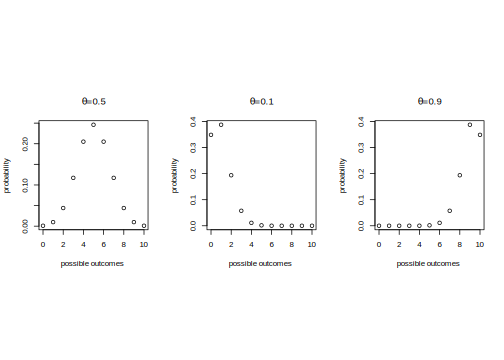
\includegraphics{bookdown_files/figure-latex/binomplot-1.pdf}
\caption{\label{fig:binomplot}Probability mass functions of a binomial distribution assuming 10 trials, with 50\%, 10\%, and 90\% probability of success.}
\end{figure}

\BeginKnitrBlock{rmdnote}
to-do bar or line graphs above, instead of points
\EndKnitrBlock{rmdnote}

The probability mass function for the binomial is written as follows.

\begin{equation}
\hbox{Binomial}(k|n,\theta) = 
\binom{n}{k} \theta^{k} (1-\theta)^{n-k}
\end{equation}

Here, \(n\) represents the total number of trials, \(k\) the number of successes (this could range from 0 to 10), and \(\theta\) the probability of success. The term \(\binom{n}{k}\), pronounced n-choose-k, represents the number of ways in which one can choose \(k\) successes out of \(n\) trials. For example, 1 success out of 10 can occur in 10 possible ways: the very first trial could be a 1, the secone trial could be a 1, etc.
The term \(\binom{n}{k}\) expands to \(\frac{n!}{k!(n-k)!}\). In \texttt{R}, it is computed using the function \texttt{choose(n,k)}, with \(n\) and \(k\) representing positive integer values.

When we want to express the fact that the data is assumed to be generated from a Binomial random variable, we will write \(Y \sim Binomial(n,\theta)\), where \(\sim\) should be read as ``is being generated from''. If the data is generated from a random variable that has some other probability distribution \(f(\theta)\), we will write \(Y\sim f(\theta)\).

\hypertarget{the-mean-and-variance-of-the-binomial-distribution}{%
\subsection{The mean and variance of the Binomial distribution}\label{the-mean-and-variance-of-the-binomial-distribution}}

It is possible to analytically compute the mean and variance of the PMF associated with the Binomial random variable \(Y\). Without getting into the details of how these are derived mathematically, we just state here that the mean of \(Y\) (also called the expectation, conventionally written \(E[Y]\)) and variance of \(Y\) (written \(Var(Y)\)) of a Binomial distribution with parameter \(\theta\) and \(n\) trials are \(E[Y] = n\theta\) and \(Var(Y) = n\theta (1-\theta)\).

Of course, \(n\) is a fixed number because we decide on the total number of trials before running the experiment. In the PMF \(\theta\) is also a fixed value; the only variable in a PMF is \(k\). In real experimental situations we never know the true value of \(\theta\). But \(\theta\) can be estimated from the data. From the observed data, we can compute the estimate of \(\theta\), \(\hat \theta=k/n\). The quantity \(\hat \theta\) is the observed proportion of successes, and is called the \textbf{maximum likelihood estimate} of the true (but unknown) expectation E{[}Y{]}. Once we have estimated \(\theta\) in this way, we can also obtain an estimate (also a maximum likelihood estimate) of the variance by computing \(n\theta (1-\theta)\). These estimates are then used for statistical inference.

What does the term ``maximum likelihood estimate'' mean? The term \textbf{likelihood} refers to the Binomial distribution function, i.e., the PMF we saw above, \(p(k|n,\theta)\). Recall that the PMF assumes that \(\theta\) and \(n\) are fixed, and \(k\) will vary from 0 to 10 when the experiment is repeated multiple times. The likelihood function is the same function as the PMF, \(p(k|n,\theta)\), but assumes that the data is fixed and only \(\theta\) varies (from 0 to 1).

For example, suppose you record \(n=10\) trials, and observe \(k=7\) successes. What is the probability of observing \(7\) successes out of \(10\)? We need the Binomial distribution to compute this value:

\begin{equation}
\hbox{Binomial}(k=7|n=10,\theta) = 
\binom{10}{7} \theta^{7} (1-\theta)^{10-7}
\end{equation}

Once we have observed the data (k=7 successes), both \(n\) and \(k\) are fixed. The only variable in the above equation now is \(\theta\): the above function is now only dependent on the value of \(\theta\).

When the data are fixed, the probability mass function is only dependent on the value of the parameter \(\theta\), and is called a \textbf{likelihood function}. It is therefore often expressed as a function of \(\theta\):

\(p( k=7, n=10 | \theta) = \mathcal{L}(\theta)\)

Since the PMF and the likelihood refer to the same function seen in two different ways, sometimes the likelihood is written \(p(\theta | k=7, n=10)\) to distinguish it from the PMF, which has the data appearing first (\(p(k|n,\theta)\)). We will write both the PMF and the likelihood identically in this book; context will disambiguate what we are referring to.

If we now plot the likelihood function for all possible values of \(\theta\) ranging from \(0\) to \(1\), we get the plot shown in Figure \ref{fig:binomlik}.

\begin{figure}
\centering
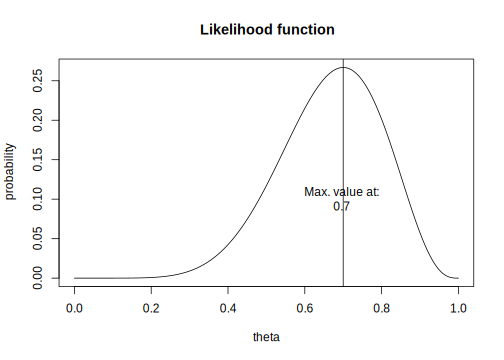
\includegraphics{bookdown_files/figure-latex/binomlik-1.pdf}
\caption{\label{fig:binomlik}The likelihood function for 7 successes out of 10.}
\end{figure}

\BeginKnitrBlock{rmdnote}
DS comment: do we want to show the code for computing all likelihood values? (maybe this comes later?)
\EndKnitrBlock{rmdnote}

What is important about this plot is that it shows that, given the data, the maximum point is at the point \(0.7\), which corresponds to the estimated mean using the formula shown above: \(k/n = 7/10\). Thus, the maximum likelihood estimate (MLE) gives us the most likely value that the parameter \(\theta\) has, given the data.

It is crucial to note here that the phrase ``most likely'' here does not mean that the MLE from a \emph{particular} sample of data invariably gives us an accurate estimate of \(\theta\). For example, if we run our experiment for \(10\) trials and get \(1\) success out of \(10\), the MLE is \(0.10\). We could have happened to observe only one success out of ten even if the true \(\theta\) were \(0.5\). The MLE would however give an accurate estimate of the true parameter as \(n\) approaches infinity.

\hypertarget{what-information-does-a-probability-distribution-provide}{%
\subsection{What information does a probability distribution provide?}\label{what-information-does-a-probability-distribution-provide}}

In Bayesian data analysis, we will constantly be asking the question: what information does a probability distribution give us? In particular, we will treat each parameter \(\theta\) as a random variable; this will raise questions like: ``what is the probability that the parameter \(\theta\) lies between two values \(a\) and \(b\);''what is the range over which we can be 95\% certain that the true value of the parameter lies"? In order to be able to answer questions like these, we need to know what information we can obtain once we have a probability distribution, and how to extract this information. We therefore discuss the different kinds of information we can obtain from a probability distribution. For now we focus only on the Binomial random variable discussed above.

\hypertarget{compute-the-probability-of-a-particular-outcome-discrete-case-only}{%
\subsubsection{Compute the probability of a particular outcome (discrete case only)}\label{compute-the-probability-of-a-particular-outcome-discrete-case-only}}

The Binomial distribution shown in Figure \ref{fig:binomplot} already shows the probability of each possible outcome under a different value for \(\theta\). In R, there is a built-in function that allows us to calculate the probability of \(k\) successes out of \(n\), given a particular value of \(k\) (this number constitutes our data), the number of trials \(n\), and given a particular value of \(\theta\); this is the \texttt{dbinom} function. For example, the probability of 5 successes out of 10 when \(\theta\) is 0.5 is:

\begin{Shaded}
\begin{Highlighting}[]
\KeywordTok{dbinom}\NormalTok{(}\DecValTok{5}\NormalTok{,}\DataTypeTok{size=}\DecValTok{10}\NormalTok{,}\DataTypeTok{prob=}\FloatTok{0.5}\NormalTok{)}
\end{Highlighting}
\end{Shaded}

\begin{verbatim}
## [1] 0.25
\end{verbatim}

The probabilities of success when \(\theta\) is 0.1 or 0.9 can be computed by replacing 0.5 above by each of these probabilities. One can just do this by giving \texttt{dbinom} a vector of probabilities:

\begin{Shaded}
\begin{Highlighting}[]
\KeywordTok{dbinom}\NormalTok{(}\DecValTok{5}\NormalTok{,}\DataTypeTok{size=}\DecValTok{10}\NormalTok{,}\DataTypeTok{prob=}\KeywordTok{c}\NormalTok{(}\FloatTok{0.1}\NormalTok{,}\FloatTok{0.9}\NormalTok{))}
\end{Highlighting}
\end{Shaded}

\begin{verbatim}
## [1] 0.0015 0.0015
\end{verbatim}

Note that the probability of a particular outcome is only computable in the discrete case; in the continuous case, this probability will always be zero (we discuss this when we turn to continuous probability distributions below).

\hypertarget{compute-the-cumulative-probability-of-k-or-less-more-than-k-successes}{%
\subsubsection{Compute the cumulative probability of k or less (more) than k successes}\label{compute-the-cumulative-probability-of-k-or-less-more-than-k-successes}}

Using the \texttt{dbinom} function, we can compute the cumulative probability of obtaining 1 or less, 2 or less successes etc. This is done through a simple summation procedure:

\begin{Shaded}
\begin{Highlighting}[]
\CommentTok{## the cumulative probability of obtaining}
\CommentTok{## 0, 1, or 2 successes out of 10,}
\CommentTok{## with theta=0.5:}
\KeywordTok{dbinom}\NormalTok{(}\DecValTok{0}\NormalTok{,}\DataTypeTok{size=}\DecValTok{10}\NormalTok{,}\DataTypeTok{prob=}\FloatTok{0.5}\NormalTok{)}\OperatorTok{+}\KeywordTok{dbinom}\NormalTok{(}\DecValTok{1}\NormalTok{,}\DataTypeTok{size=}\DecValTok{10}\NormalTok{,}\DataTypeTok{prob=}\FloatTok{0.5}\NormalTok{)}\OperatorTok{+}
\StringTok{  }\KeywordTok{dbinom}\NormalTok{(}\DecValTok{2}\NormalTok{,}\DataTypeTok{size=}\DecValTok{10}\NormalTok{,}\DataTypeTok{prob=}\FloatTok{0.5}\NormalTok{)}
\end{Highlighting}
\end{Shaded}

\begin{verbatim}
## [1] 0.055
\end{verbatim}

Mathematically, we could write the above summation as:

\begin{equation}
\sum_{k=0}^2 \binom{n}{k} \theta^{k} (1-\theta)^{n-k} 
\end{equation}

An alternative to the cumbersome addition in the R code above is this more compact statement, which closely mimics the above mathematical expression:

\begin{Shaded}
\begin{Highlighting}[]
\KeywordTok{sum}\NormalTok{(}\KeywordTok{dbinom}\NormalTok{(}\DecValTok{0}\OperatorTok{:}\DecValTok{2}\NormalTok{,}\DataTypeTok{size=}\DecValTok{10}\NormalTok{,}\DataTypeTok{prob=}\FloatTok{0.5}\NormalTok{))}
\end{Highlighting}
\end{Shaded}

\begin{verbatim}
## [1] 0.055
\end{verbatim}

R has a built-in function called \texttt{pbinom} that does this summation for us. If we want to know the probability of \(2\) or less successes as in the above example, we can write:

\begin{Shaded}
\begin{Highlighting}[]
\KeywordTok{pbinom}\NormalTok{(}\DecValTok{2}\NormalTok{,}\DataTypeTok{size=}\DecValTok{10}\NormalTok{,}\DataTypeTok{prob=}\FloatTok{0.5}\NormalTok{,}\DataTypeTok{lower.tail=}\OtherTok{TRUE}\NormalTok{)}
\end{Highlighting}
\end{Shaded}

\begin{verbatim}
## [1] 0.055
\end{verbatim}

The specification \texttt{lower.tail=TRUE} ensures that the summation goes from \(2\) to numbers smaller than \(2\) (which lie in the lower tail of the distribution in Figure \ref{fig:binomplot}). If we wanted to know what the probability is of obtaining \(2\) or more successes out of \(10\), we can set \texttt{lower.tail} to \texttt{FALSE}:

\begin{Shaded}
\begin{Highlighting}[]
\KeywordTok{pbinom}\NormalTok{(}\DecValTok{2}\NormalTok{,}\DataTypeTok{size=}\DecValTok{10}\NormalTok{,}\DataTypeTok{prob=}\FloatTok{0.5}\NormalTok{,}\DataTypeTok{lower.tail=}\OtherTok{FALSE}\NormalTok{)}
\end{Highlighting}
\end{Shaded}

\begin{verbatim}
## [1] 0.95
\end{verbatim}

The cumulative distribution function or CDF can be plotted by computing the cumulative probabilities for any value \(k\) or less than \(k\), where \(k\) ranges from \(0\) to \(10\) in our running example. The CDF is shown in Figure \ref{fig:binomcdf}.

\begin{figure}
\centering
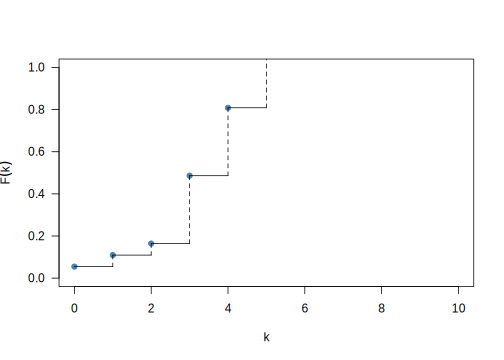
\includegraphics{bookdown_files/figure-latex/binomcdf-1.pdf}
\caption{\label{fig:binomcdf}The cumulative distribution function for a Binomial distribution assuming 10 trials, with 50\% probability of success.}
\end{figure}

\hypertarget{compute-the-inverse-of-the-cumulative-distribution-function-the-quantile-function}{%
\subsubsection{Compute the inverse of the cumulative distribution function (the quantile function)}\label{compute-the-inverse-of-the-cumulative-distribution-function-the-quantile-function}}

We can also find out the value of the variable \(k\) (the quantile) such that the probability of obtaining \(k\) or less than \(k\) successes is some specific probability value \(p\). If we switch the x and y axes of Figure \ref{fig:binomcdf}, we obtain another very useful function, the inverse CDF.

The inverse of the CDF (known as the quantile function in R because it returns the quantile, the value k) is available in R as the function \texttt{qbinom}. The usage is as follows: to find out what the value \(k\) of the outcome is such that the probability of obtaining \(k\) or less successes is \(0.37\), type:

\begin{Shaded}
\begin{Highlighting}[]
\KeywordTok{qbinom}\NormalTok{(}\FloatTok{0.37}\NormalTok{,}\DataTypeTok{size=}\DecValTok{10}\NormalTok{,}\DataTypeTok{prob=}\FloatTok{0.5}\NormalTok{)}
\end{Highlighting}
\end{Shaded}

\begin{verbatim}
## [1] 4
\end{verbatim}

\BeginKnitrBlock{rmdnote}
to-do: explain why qbinom(0.77 gives 5 as an answer and not 4)
\EndKnitrBlock{rmdnote}

\BeginKnitrBlock{rmdnote}
DS comment: maybe it's good to include an additional Figure for the inverse CDF and an example
\EndKnitrBlock{rmdnote}

\hypertarget{generate-simulated-data-from-a-hboxbinomialntheta-distribution}{%
\subsubsection{\texorpdfstring{Generate simulated data from a \(\hbox{Binomial}(n,\theta)\) distribution}{Generate simulated data from a \textbackslash{}hbox\{Binomial\}(n,\textbackslash{}theta) distribution}}\label{generate-simulated-data-from-a-hboxbinomialntheta-distribution}}

We can generate simulated data from a Binomial distribution by specifying the number of trials and the probability of success \(\theta\). In \texttt{R}, we do this as follows:

\begin{Shaded}
\begin{Highlighting}[]
\KeywordTok{rbinom}\NormalTok{(}\DecValTok{1}\NormalTok{,}\DataTypeTok{size=}\DecValTok{10}\NormalTok{,}\DataTypeTok{prob=}\FloatTok{0.5}\NormalTok{)}
\end{Highlighting}
\end{Shaded}

\begin{verbatim}
## [1] 7
\end{verbatim}

\BeginKnitrBlock{rmdnote}
to-do: introduce Bernoulli here and link it with the code below
\EndKnitrBlock{rmdnote}

The above code generates the number of successes in an experiment with \(10\) trials. Repeatedly run the above code; you will get different sequences each time. For each generated sequence, one can calculate the number of successes by just summing up the vector, or computing its mean and multiplying by the number of trials, here \(10\):

\begin{Shaded}
\begin{Highlighting}[]
\NormalTok{y<-}\KeywordTok{rbinom}\NormalTok{(}\DecValTok{10}\NormalTok{,}\DataTypeTok{size=}\DecValTok{1}\NormalTok{,}\DataTypeTok{prob=}\FloatTok{0.5}\NormalTok{)}
\KeywordTok{mean}\NormalTok{(y)}\OperatorTok{*}\DecValTok{10}\NormalTok{ ; }\KeywordTok{sum}\NormalTok{(y)}
\end{Highlighting}
\end{Shaded}

\begin{verbatim}
## [1] 6
\end{verbatim}

\begin{verbatim}
## [1] 6
\end{verbatim}

\hypertarget{continuous-random-variables-an-example-using-the-normal-distribution}{%
\section{Continuous random variables: An example using the Normal distribution}\label{continuous-random-variables-an-example-using-the-normal-distribution}}

We will now revisit the idea of the random variable using a continuous distribution. Imagine that you have a vector of reading time data \(y\) measured in milliseconds and coming from a Normal distribution. The Normal distribution is defined in terms of two parameters: a mean value \(\mu\), which determines its center, and the variance \(\sigma^2\), which determines how much spread there is around this center point.

The probability density function (PDF) of the Normal distribution is defined as follows:

\begin{equation}
Normal(y|\mu,\sigma)=f(y)= \frac{1}{\sqrt{2\pi \sigma^2}} \exp \left(-\frac{(y-\mu)^2}{2\sigma^2} \right)
\end{equation}

Here, \(\mu\) is some true, unknown mean, and \(\sigma^2\) is some true, unknown variance of the Normal distribution that the reading times have been sampled from. There is a built-in function in R that computes the above function once we specify the mean \(\mu\) and the standard deviation \(\sigma\) (in R, this parameter is specified in terms of the standard deviation rather than the variance).

Figure \ref{fig:normdistrn} visualizes the Normal distribution for particular values of \(\mu\) and \(\sigma\), as a PDF (using \texttt{dnorm}), a CDF (using \texttt{pnorm}), and the inverse CDF (using \texttt{qnorm}). It is clear from the figure that these are three different ways of looking at the same information.

\begin{figure}
\centering
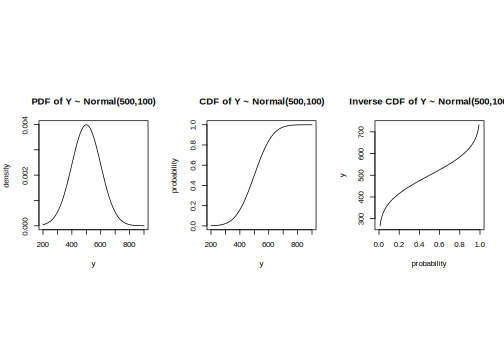
\includegraphics{bookdown_files/figure-latex/normdistrn-1.pdf}
\caption{\label{fig:normdistrn}The PDF, CDF, and inverse CDF for the \(Normal(\mu=500,\sigma=100)\).}
\end{figure}

\BeginKnitrBlock{rmdnote}
to-do: Maybe this is the place to mention some interesting properties like:
Normal(mu, sigma) = mu + Normal(0,1) * sigma
(We'll use this property a lot later when we code in Stan)
\EndKnitrBlock{rmdnote}

As in the discrete example, the PDF, CDF, and inverse of the CDF allow us to ask questions like:

\begin{itemize}
\tightlist
\item
  \textbf{What is the probability of observing values between \(a\) and \(b\) from a Normal distribution with mean \(\mu\) and standard deviation \(\sigma\)}? Using the above example, we can ask what the probability of observing values between 200 and 700 ms:
\end{itemize}

\begin{Shaded}
\begin{Highlighting}[]
\KeywordTok{pnorm}\NormalTok{(}\DecValTok{700}\NormalTok{,}\DataTypeTok{mean=}\DecValTok{500}\NormalTok{,}\DataTypeTok{sd=}\DecValTok{100}\NormalTok{)}\OperatorTok{-}\KeywordTok{pnorm}\NormalTok{(}\DecValTok{200}\NormalTok{,}\DataTypeTok{mean=}\DecValTok{500}\NormalTok{,}\DataTypeTok{sd=}\DecValTok{100}\NormalTok{)}
\end{Highlighting}
\end{Shaded}

\begin{verbatim}
## [1] 0.98
\end{verbatim}

\BeginKnitrBlock{rmdnote}
to-do: add figure illustrating the above
\EndKnitrBlock{rmdnote}

Notice here that the probability of any point value in a PDF is always \(0\). This is because the probability in a continuous probability distribution is the area under the curve, and the area at any point on the x-axis is always \(0\). The implication here is that we can only ask about probabilities between two different points; e.g., the probability that \(Y\) lies between \(a\) and \(b\), or \(P(a<Y<b)\).

\begin{itemize}
\tightlist
\item
  \textbf{What is the quantile \(q\) such that the probability is \(p\) of observing that value \(q\) or something less (or more) than it}? For example, we can work out the quantile \(q\) such that the probability of observing \(q\) or something less than it is 0.975, in the Normal(500,100) distribution. Formally, we would write this as \(P(Y<a)\).
\end{itemize}

\begin{Shaded}
\begin{Highlighting}[]
\KeywordTok{qnorm}\NormalTok{(}\FloatTok{0.975}\NormalTok{,}\DataTypeTok{mean=}\DecValTok{500}\NormalTok{,}\DataTypeTok{sd=}\DecValTok{100}\NormalTok{)}
\end{Highlighting}
\end{Shaded}

\begin{verbatim}
## [1] 696
\end{verbatim}

The above output says that the probability that the random variable is less than \(q=695\) is 97.5\%.

\begin{itemize}
\tightlist
\item
  \textbf{Generating simulated data}. Given a vector of \(n\) independent and identically distributed data \(y\), i.e., given that each data point is being generated independently from \(Y \sim Normal(\mu,\sigma)\) for some values of the parameters, the maximum likelihood estimates for the expectation and variance\footnote{R will compute variance by dividing by \(n-1\), not \(n\); this is because dividing by \(n\) gives a biased estimate. This is not an important detail for our purposes, and in any case for large \(n\) it doesn't really matter whether one divides by \(n\) or \(n-1\).} are:
\end{itemize}

\begin{equation}
\bar{y} =  \frac{\sum_{i=1}^n y_i}{n} 
\end{equation}

\begin{equation}
Var(y) = \frac{\sum_{i=1}^n (y_i-
\bar{y})^2}{n}
\end{equation}

For example, we can generate \(10\) data points using the \texttt{rnorm} function, and then compute the mean and variance from the simulated data:

\begin{Shaded}
\begin{Highlighting}[]
\NormalTok{y<-}\KeywordTok{rnorm}\NormalTok{(}\DecValTok{10}\NormalTok{,}\DataTypeTok{mean=}\DecValTok{500}\NormalTok{,}\DataTypeTok{sd=}\DecValTok{100}\NormalTok{)}
\KeywordTok{mean}\NormalTok{(y);}\KeywordTok{var}\NormalTok{(y)}
\end{Highlighting}
\end{Shaded}

\begin{verbatim}
## [1] 560
\end{verbatim}

\begin{verbatim}
## [1] 6778
\end{verbatim}

Again, the sample mean and sample variance computed from a particular data-set need not necessarily be close to the true values of the respective parameters.

\hypertarget{an-important-distinction-probability-vs.density-in-a-continuous-random-variable}{%
\subsection{An important distinction: probability vs.~density in a continuous random variable}\label{an-important-distinction-probability-vs.density-in-a-continuous-random-variable}}

In continuous distributions like the Normal discussed above, it is important to understand that the probability density function or PDF, \(p(y| \mu, \sigma)\) defines a mapping from the \(y\) values (the possible values that the data can have) to a quantity called the density of each possible value. We can see this function in action when we use \texttt{dnorm} to compute, say, the density value corresponding to \(y=1\) in the \(Normal(\mu=0,\sigma=1)\) distribution.

\begin{Shaded}
\begin{Highlighting}[]
\CommentTok{## density:}
\KeywordTok{dnorm}\NormalTok{(}\DecValTok{1}\NormalTok{,}\DataTypeTok{mean=}\DecValTok{0}\NormalTok{,}\DataTypeTok{sd=}\DecValTok{1}\NormalTok{)}
\end{Highlighting}
\end{Shaded}

\begin{verbatim}
## [1] 0.24
\end{verbatim}

The quantity above is \emph{not} the probability of observing 1 in this distribution. As mentioned earlier, probability in a continuous distribution is the area under the curve, and this area will always be zero at any point value. If we want to know the probability of obtaining values between an upper and lower bound \(b\) and \(a\), i.e., \(P(a<Y<b)\) where these are two distinct values, we must use the \texttt{pnorm} function. For example, the probability of observing a value between +2 and -2 in a Normal distribution with mean 0 and standard deviation 1 is:

\begin{Shaded}
\begin{Highlighting}[]
\KeywordTok{pnorm}\NormalTok{(}\DecValTok{2}\NormalTok{,}\DataTypeTok{mean=}\DecValTok{0}\NormalTok{,}\DataTypeTok{sd=}\DecValTok{1}\NormalTok{)}\OperatorTok{-}\KeywordTok{pnorm}\NormalTok{(}\OperatorTok{-}\DecValTok{2}\NormalTok{,}\DataTypeTok{mean=}\DecValTok{0}\NormalTok{,}\DataTypeTok{sd=}\DecValTok{1}\NormalTok{)}
\end{Highlighting}
\end{Shaded}

\begin{verbatim}
## [1] 0.95
\end{verbatim}

Notice that the situation is different in discrete random variables. These have a probability mass function (PMF) associated with them---the Binomial distribution that we saw earlier is an example. There, the PMF maps the possible \(y\) values to the probabilities of those values occurring. That is why, in the Binomial distribution, the probability of observing exactly 2 successes when sampling from a \(Binomial(n=10,\theta=0.5)\) can be computed using either \texttt{dbinom} or \texttt{pbinom}:

\begin{Shaded}
\begin{Highlighting}[]
\KeywordTok{dbinom}\NormalTok{(}\DecValTok{2}\NormalTok{,}\DataTypeTok{size=}\DecValTok{10}\NormalTok{,}\DataTypeTok{prob=}\FloatTok{0.5}\NormalTok{)}
\end{Highlighting}
\end{Shaded}

\begin{verbatim}
## [1] 0.044
\end{verbatim}

\begin{Shaded}
\begin{Highlighting}[]
\KeywordTok{pbinom}\NormalTok{(}\DecValTok{2}\NormalTok{,}\DataTypeTok{size=}\DecValTok{10}\NormalTok{,}\DataTypeTok{prob=}\FloatTok{0.5}\NormalTok{)}\OperatorTok{-}\KeywordTok{pbinom}\NormalTok{(}\DecValTok{1}\NormalTok{,}\DataTypeTok{size=}\DecValTok{10}\NormalTok{,}\DataTypeTok{prob=}\FloatTok{0.5}\NormalTok{)}
\end{Highlighting}
\end{Shaded}

\begin{verbatim}
## [1] 0.044
\end{verbatim}

In the second line of code above, we are computing the cumulative probability of observing two or less successes, minus the probability of observing one or less successes. This gives us the probability of observing exactly two successes. The \texttt{dbinom} gives us this same information.

\hypertarget{an-important-concept-the-marginal-likelihood-integrating-out-a-parameter}{%
\section{An important concept: The marginal likelihood (integrating out a parameter)}\label{an-important-concept-the-marginal-likelihood-integrating-out-a-parameter}}

Here, we introduce a concept that will turn up many times in this book. The concept we unpack here is called ``integrating out a parameter''. We will need this when we encounter Bayes' rule in the next chapter, and when we use Bayes factors later in the book.

Integrating out a parameter refers to the following situation. Suppose we have a Binomial random variable \(Y\) with PMF \(p(Y)\). Suppose also that this PMF is defined in terms of parameter \(\theta\) that can have only three possible values, \(0.1, 0.5, 0.9\), each with equal probability. In other words, the probability that \(\theta\) is \(0.1, 0.5,\) or \(0.9\) is 1/3 each.

We stick with our earlier example of \(n=10\) trials and \(k=8\) successes.
The \textbf{likelihood function} then is

\begin{equation}
p(k=8|n=10,\theta) = \binom{10}{8} \theta^8 (1-\theta)^{2}
\end{equation}

There is a related concept of \textbf{marginal likelihood}, which we can write here as \(p(k=8,n=10)\). Marginal likelihood is the likelihood computed by ``marginalizing'' out the parameter \(\theta\): for each possible value that the parameter \(\theta\) can have, we compute the likelihood at that value and multiply that likelihood with the probability of that \(\theta\) value occurring. Then we sum up each of the products computed in this way. Mathematically, this means that we carry out the following operation.

In our example, there are three possible values of \(\theta\),
call them \(\theta_1=0.1\), \(\theta_2=0.5\), and \(\theta_3=0.9\). Each has probability \(1/3\); so \(p(\theta_1)=p(\theta_2)=p(\theta_3)=1/3\). Given this information, we can compute the marginal likelihood as follows:

\begin{equation}
\begin{split}
p(k=8,n=10) =& \binom{10}{8} \theta_1^8 (1-\theta_1)^{2} \times p(\theta_1) \\
            +& \binom{10}{8} \theta_2^8 (1-\theta_2)^{2}\times p(\theta_2) \\
            +& \binom{10}{8} \theta_3^8 (1-\theta_3)^{2}\times p(\theta_3)\\
\end{split}
\end{equation}

Writing the \(\theta\) values and their probabilities, we get:

\begin{equation}
\begin{split}
p(k=8,n=10) =& \binom{10}{8} 0.1^8 (1-0.1)^{2} \times \frac{1}{3} \\
            +& \binom{10}{8} \theta_2^8 (1-\theta_2)^{2}\times \frac{1}{3} \\
            +& \binom{10}{8} \theta_3^8 (1-\theta_3)^{2}\times \frac{1}{3}\\
\end{split}
\end{equation}

We can simplify this summation by collecting together the common terms:

\begin{equation}
\begin{split}
p(k=8,n=10) =& \frac{1}{3} [\binom{10}{8}  0.1^8 (1-0.1)^{2} \\
+& \binom{10}{8} \theta_2^8 (1-\theta_2)^{2} \\
+& \binom{10}{8} \theta_3^8 (1-\theta_3)^{2}] \\
=& 0.06 \\
\end{split}
\end{equation}

Thus, a marginal likelihood is a kind of weighted sum of the likelihood, weighted by the possible values of the parameter.\footnote{Where does the above formula come from? It falls out from the law of total probability; see \citet{blitzstein2014introduction} for a detailed exposition.}

The above example was contrived, because we stated that the parameter \(\theta\) has only three possible values. In reality, because the parameter \(\theta\) can have all possible values between 0 and 1, the summation has to be done over a continuous space \([0,1]\). The way this summation is expressed in mathematics is through the integral symbol:

\begin{equation}
p(k=8,n=10) = \int_0^1 \binom{10}{8} \theta^8 (1-\theta)^{2}\, d\theta
\end{equation}

This statement is saying exactly what we computed above, except that the summation is being done over a continuous space ranging from 0 to 1. We say that the parameter \(\theta\) has been integrated out, or marginalized. Integrating out a parameter will be a very common operation in this book, but fortunately we will never have to do the calculation ourselves. For the above case, we can easily compute the integral in R:

\begin{Shaded}
\begin{Highlighting}[]
\NormalTok{BinLik<-}\ControlFlowTok{function}\NormalTok{(theta)\{}
  \KeywordTok{choose}\NormalTok{(}\DecValTok{10}\NormalTok{,}\DecValTok{8}\NormalTok{)}\OperatorTok{*}\NormalTok{theta}\OperatorTok{^}\DecValTok{8} \OperatorTok{*}\StringTok{ }\NormalTok{(}\DecValTok{1}\OperatorTok{-}\NormalTok{theta)}\OperatorTok{^}\DecValTok{2}
\NormalTok{\}}
\KeywordTok{integrate}\NormalTok{(BinLik,}\DataTypeTok{lower=}\DecValTok{0}\NormalTok{,}\DataTypeTok{upper=}\DecValTok{1}\NormalTok{)}\OperatorTok{$}\NormalTok{value}
\end{Highlighting}
\end{Shaded}

\begin{verbatim}
## [1] 0.091
\end{verbatim}

This completes our discussion of random variables and probability distributions. We now summarize what we have learnt so far.

\hypertarget{summary-of-useful-r-functions-relating-to-distributions}{%
\section{Summary of useful R functions relating to distributions}\label{summary-of-useful-r-functions-relating-to-distributions}}

Table \ref{tab:dpqrfunctions} summarizes the different functions relating to PMFs and PDFs, using the Binomial and Normal as examples.

\begin{longtable}[]{@{}lcc@{}}
\caption{\label{tab:dpqrfunctions} Important R functions relating to random variables.}\tabularnewline
\toprule
& Discrete & Continuous\tabularnewline
\midrule
\endfirsthead
\toprule
& Discrete & Continuous\tabularnewline
\midrule
\endhead
Example: & Binomial(\(y|n,\theta\)) & Normal(\(y|\mu,\sigma\))\tabularnewline
Likelihood function & dbinom & dnorm\tabularnewline
Prob Y=y & dbinom & always 0\tabularnewline
Prob \(Y\geq y, Y\leq y, y_1<Y<y_2\) & pbinom & pnorm\tabularnewline
Inverse CDF & qbinom & qnorm\tabularnewline
Generate simulated data & rbinom & rnorm\tabularnewline
\bottomrule
\end{longtable}

Later on, we will use other distributions, such as the Uniform, Beta, etc., and each of these has their own set of d-p-q-r functions in R. The appendix summarizes the properties of the distributions that we will need in this book.

\hypertarget{summary-of-concepts-introduced-in-this-chapter}{%
\section{Summary of concepts introduced in this chapter}\label{summary-of-concepts-introduced-in-this-chapter}}

\BeginKnitrBlock{rmdnote}
to-do: add summary
\EndKnitrBlock{rmdnote}

\hypertarget{further-reading}{%
\section{Further reading}\label{further-reading}}

A quick review of the mathematical foundations needed for statistics is available in the short book by \citet{fox2009mathematical}. \citet{morin2016probability} and \citet{blitzstein2014introduction} are accessible introductions to probability theory.

\hypertarget{exercises}{%
\section{Exercises}\label{exercises}}

\hypertarget{practice-using-the-pnorm-function}{%
\subsection{\texorpdfstring{Practice using the \texttt{pnorm} function}{Practice using the pnorm function}}\label{practice-using-the-pnorm-function}}

\hypertarget{part-1}{%
\subsubsection{Part 1}\label{part-1}}

Given a normal distribution with mean \texttt{61} and standard deviation \texttt{101}, use the pnorm function to calculate the probability of obtaining values between \texttt{217} and \texttt{-95} from this distribution.

\hypertarget{part-2}{%
\subsubsection{Part 2}\label{part-2}}

Calculate the following probabilities.
Given a normal distribution with mean \texttt{51} and standard deviation \texttt{4}, what is the probability of getting

\begin{itemize}
\tightlist
\item
  a score of \texttt{48} or less
\item
  a score of \texttt{48} or more
\item
  a score of \texttt{56} or more
\end{itemize}

\hypertarget{part-3}{%
\subsubsection{Part 3}\label{part-3}}

Given a normal distribution with mean \texttt{53} and standard deviation \texttt{4}, what is the probability of getting

\begin{itemize}
\tightlist
\item
  a score of \texttt{48} or less.
\item
  a score between \texttt{50} and \texttt{56}.
\item
  a score of \texttt{mu+1} or more.
\end{itemize}

\hypertarget{practice-using-the-qnorm-function}{%
\subsection{\texorpdfstring{Practice using the \texttt{qnorm} function}{Practice using the qnorm function}}\label{practice-using-the-qnorm-function}}

\hypertarget{part-1-1}{%
\subsubsection{Part 1}\label{part-1-1}}

Consider a normal distribution with mean 1 and standard deviation 1.

Compute the lower and upper boundaries such that:

\begin{itemize}
\tightlist
\item
  the area (the probability) to the left of the lower boundary is \texttt{0.27}.
\item
  the area (the probability) to the left of the upper boundary is \texttt{0.91}.
\end{itemize}

\hypertarget{part-2-1}{%
\subsubsection{Part 2}\label{part-2-1}}

Given a normal distribution with mean \texttt{56.93} and standard deviation \texttt{0.74}. There exist two quantiles, the lower quantile q1 and the upper quantile q2, that are equidistant from the mean \texttt{56.93}, such that the area under the curve of the Normal probability between q1 and q2 is \texttt{85}\%. Find q1 and q2.

\hypertarget{practice-using-qt}{%
\subsection{\texorpdfstring{Practice using \texttt{qt}}{Practice using qt}}\label{practice-using-qt}}

Take an independent random sample of size \texttt{144} from a normal distribution
with mean \texttt{133}, and standard deviation \texttt{54}. Next, we are going to pretend we don't know the population parameters (the mean and standard deviation). We compute the MLEs of the mean and standard deviation using the data and get the sample mean \texttt{130.63} and the sample standard deviation \texttt{50.05}.

\begin{itemize}
\tightlist
\item
  Compute the estimated standard error using the sample standard deviation provided above.
\item
  What are your degrees of freedom for the relevant t-distribution?
\item
  Calculate the \textbf{absolute} critical t-value for a 95\% confidence interval using the relevant degrees of freedom you just wrote above.
\item
  Next, compute the lower bound of the 95\% confidence interval using the estimated standard error and the critical t-value.
\item
  Finally, compute the upper bound of the 95\% confidence interval using the estimated standard error and the critical t-value.
\end{itemize}

\hypertarget{maximum-likelihood-estimation-1}{%
\subsection{Maximum likelihood estimation 1}\label{maximum-likelihood-estimation-1}}

Given the data point \texttt{9.08}.
The function \texttt{dnorm} gives the likelihood given a data point (or multiple data points) and a value for the mean and the standard deviation (sd). Using \texttt{dnorm}, compute

\begin{itemize}
\tightlist
\item
  the likelihood of the data point \texttt{9.08} assuming a mean of \texttt{12} and standard deviation 5.
\item
  the likelihood of the data point \texttt{9.08} assuming a mean of \texttt{11} and standard deviation 5.
\item
  the likelihood of the data point \texttt{9.08} assuming a mean of \texttt{10} and standard deviation 5.
\item
  the likelihood of the data point \texttt{9.08} assuming a mean of \texttt{9} and standard deviation 5.
\end{itemize}

\hypertarget{maximum-likelihood-estimation-2}{%
\subsection{Maximum likelihood estimation 2}\label{maximum-likelihood-estimation-2}}

You are given \(10\) independent and identically distributed data points that are assumed to come from a Normal distribution with unknown mean and unknown standard deviation:

\begin{Shaded}
\begin{Highlighting}[]
\NormalTok{x}
\end{Highlighting}
\end{Shaded}

\begin{verbatim}
##  [1] 504 503 497 487 507 506 492 484 502 497
\end{verbatim}

The function \texttt{dnorm} gives the likelihood given multiple data points and a value for the mean and the standard deviation. The log-likelihood can be computed by typing \texttt{dnorm(...,log=TRUE)}.

The product of the likelihoods for two independent data points can be computed like this: Suppose we have two independent and identically distributed data points 5 and 10. Then, assuming that the Normal distribution they come from has mean 10 and standard deviation 2, the joint likelihood of these is:

\begin{Shaded}
\begin{Highlighting}[]
\KeywordTok{dnorm}\NormalTok{(}\DecValTok{5}\NormalTok{,}\DataTypeTok{mean=}\DecValTok{10}\NormalTok{,}\DataTypeTok{sd=}\DecValTok{2}\NormalTok{)}\OperatorTok{*}\KeywordTok{dnorm}\NormalTok{(}\DecValTok{10}\NormalTok{,}\DataTypeTok{mean=}\DecValTok{10}\NormalTok{,}\DataTypeTok{sd=}\DecValTok{2}\NormalTok{)}
\end{Highlighting}
\end{Shaded}

\begin{verbatim}
## [1] 0.0017
\end{verbatim}

It is easier to do this on the log scale, because then one can add instead of multiplying. This is because \(\log(x\times y)= \log(x) + \log(y)\). For example:

\begin{Shaded}
\begin{Highlighting}[]
\KeywordTok{log}\NormalTok{(}\DecValTok{2}\OperatorTok{*}\DecValTok{3}\NormalTok{)}
\end{Highlighting}
\end{Shaded}

\begin{verbatim}
## [1] 1.8
\end{verbatim}

\begin{Shaded}
\begin{Highlighting}[]
\KeywordTok{log}\NormalTok{(}\DecValTok{2}\NormalTok{) }\OperatorTok{+}\StringTok{ }\KeywordTok{log}\NormalTok{(}\DecValTok{3}\NormalTok{)}
\end{Highlighting}
\end{Shaded}

\begin{verbatim}
## [1] 1.8
\end{verbatim}

So the joint log likelihood of the two data points is:

\begin{Shaded}
\begin{Highlighting}[]
\KeywordTok{dnorm}\NormalTok{(}\DecValTok{5}\NormalTok{,}\DataTypeTok{mean=}\DecValTok{10}\NormalTok{,}\DataTypeTok{sd=}\DecValTok{2}\NormalTok{,}\DataTypeTok{log=}\OtherTok{TRUE}\NormalTok{)}\OperatorTok{+}\KeywordTok{dnorm}\NormalTok{(}\DecValTok{10}\NormalTok{,}\DataTypeTok{mean=}\DecValTok{10}\NormalTok{,}\DataTypeTok{sd=}\DecValTok{2}\NormalTok{,}\DataTypeTok{log=}\OtherTok{TRUE}\NormalTok{)}
\end{Highlighting}
\end{Shaded}

\begin{verbatim}
## [1] -6.3
\end{verbatim}

Even more compactly:

\begin{Shaded}
\begin{Highlighting}[]
\KeywordTok{sum}\NormalTok{(}\KeywordTok{dnorm}\NormalTok{(}\KeywordTok{c}\NormalTok{(}\DecValTok{5}\NormalTok{,}\DecValTok{10}\NormalTok{),}\DataTypeTok{mean=}\DecValTok{10}\NormalTok{,}\DataTypeTok{sd=}\DecValTok{2}\NormalTok{,}\DataTypeTok{log=}\OtherTok{TRUE}\NormalTok{))}
\end{Highlighting}
\end{Shaded}

\begin{verbatim}
## [1] -6.3
\end{verbatim}

\begin{itemize}
\tightlist
\item
  Given the 10 data points above, calculate the maximum likelihood estimate (MLE) of the expectation.
\item
  The sum of the log-likelihoods of the data-points x, using as the mean the MLE from the sample, and standard deviation 5.
\item
  What is the sum of the log-likelihood if the mean used to compute the log-likelihood is \texttt{495.9}?
\item
  Which value for the mean, the MLE or \texttt{495.9}, gives the higher log-likelihood?
\end{itemize}

\hypertarget{introBDA}{%
\chapter{Introduction to Bayesian data analysis}\label{introBDA}}

Recall Bayes' rule: When A and B are observable events,
we can state the rule as follows:

\begin{equation}
P(A\mid B) = \frac{P(B\mid A) P(A)}{P(B)}
\label{eq:bayes-P}
\end{equation}

Given a vector of data \(y\), Bayes' rule allows us to work out the posterior distributions of the parameters of interest, which we can repesent as the vector of parameters \(\Theta\). This computation is achieved by rewriting \eqref{eq:bayes-P} as \eqref{eq:bayes}. What is different here is that Bayes' rule is written in terms of probability distributions. Here, \(p(\cdot)\) is a probability density, not the probability of a single event, which we represent above using \(P(\cdot)\).

\begin{equation}
p(\Theta|y) = \cfrac{ p(y|\Theta) \cdot p(\Theta) }{p(y)}
\label{eq:bayes}
\end{equation}

The above statement can be rewritten in words as follows:

\begin{equation}
\hbox{Posterior} = \frac{\hbox{Likelihood} \cdot \hbox{Prior}}{\hbox{Marginal Likelihood}}
\end{equation}

The terms here have the following meaning. We elaborate on each point with an example below.

\begin{itemize}
\item
  The \emph{Posterior}, \(p(\Theta|y)\) is the probability distribution of the parameters conditional on the data.
\item
  The \emph{Likelihood} is as described in chapter 1: it is the PMF (discrete case) or the PDF (continuous case) expressed a function of \(\Theta\).
\item
  The \emph{Prior} is the initial probability distribution of the parameter, before seeing the data.
\item
  The \emph{Marginal Likelihood} was introduced in chapter 1 and standardizes the posterior distribution to ensure that the area under the curve of the distribution sums to 1, that is, it ensures that the posterior is a valid probability distribution.
\end{itemize}

An example will clarify all these terms, as we explain below.

\hypertarget{sec:analytical}{%
\section{Deriving the posterior using Bayes' rule: An analytical example}\label{sec:analytical}}

Recall our cloze probability example earlier. Participants are shown sentences like

``It's raining. I'm going to take the \ldots{}''

Ten participants are asked to complete the sentence.
If \(8\) out of \(10\) participants complete the sentence with ``umbrella,'' the estimated cloze probability or predictability (given the preceding context) would be \(\frac{8}{10}=0.8\). This is the maximum likelihood estimate of the probability of producing this word; we will designate the estimate with a ``hat'' on the parameter name: \(\hat \theta=0.8\).

Notice an important point here: one shortcoming of simply writing down the proportion in this way is that it ignores the uncertainty of our measurement: \(0.8\) could come from \(10\) participants (\(\frac{8}{10}\)), \(100\) participants (\(\frac{80}{100}\)), or \(100,000\) participants (\(\frac{80000}{100000}\)). The uncertainty of the estimate \(0.8\) is different in each of these cases, and that is very relevant when drawing conclusions from data.

In the frequentist framework, the only thing we can characterize our uncertainty about is the \textbf{sampling distribution} of this parameter under imaginary repeated sampling; we can never talk about our uncertainty about the parameter's true value itself.
Thus, for a sample size of \(10\), our uncertainty of the sampling distribution would be computed by calculating the sample variance \(\sigma^2\) (here, \(n\times \hat\theta(1-\hat\theta)= 10\times 0.8 \times (1-0.8)=1.6\)), and then calculating the standard error: \(\sigma/\sqrt{n}=0.4\). Increasing the sample size will make this standard error smaller and smaller for the same estimated proportion of successes of \(0.8\). This increased precision is a statement about the uncertainty of the sampling distribution of \(\theta\) under imaginary repeated sampling; it is not an estimate of the uncertainty of \(\theta\) itself.

The Bayesian framework gives us the opportunity to talk directly about our uncertainty of the parameter itself, given the data. This is achieved by obtaining the posterior distribution of the parameter using Bayes' rule, as we show below.

\hypertarget{choosing-a-likelihood}{%
\subsection{Choosing a likelihood}\label{choosing-a-likelihood}}

Under the assumptions we have set up above, the responses follow a Binomial distribution, and so the PMF can be written as follows.

\begin{equation}
p(k|n,\theta) = \binom{n}
{k} \theta^k (1-\theta)^{n-k}
\label{eq:binom}
\end{equation}

where \(k\) indicates the number of times ``umbrella'' is given as an answer, and \(n\) the total number of answers given.

In a particular experiment that we carry out, if \(n=10\) and \(k = 8\), these data are now a fixed quantity. The PMF above now becomes a function of \(\theta\), the likelihood function:

\begin{equation}
p(k=8 | n= 10, \theta) = \binom{n}{k} \theta^8 (1-\theta)^{2}
\end{equation}

The above function is a now a continuous function of the value \(\theta\), which has possible values ranging from 0 to 1. Compare this to the PMF of the Binomial, which treats \(\theta\) as a fixed value and defines a discrete distribution over the n+1 possible discrete values \(k\) that we can observe (the possible number of successes).

It is important to pause for a moment here to appreciate the fact that the PMF and the likelihood are the same function seen from different points of view. The only difference between the two is what is considered to be fixed and what is varying. The PMF treats data as varying from experiment to experiment and \(\theta\) as fixed, whereas the likelihood function treats the data as fixed and the parameter \(\theta\) as varying.

We now turn our attention back to our main goal, which is to find out, using Bayes' rule, the posterior distribution of \(\theta\) given our data: \(p(\theta|n,k)\). In order to use Bayes' rule to calculate this posterior distribution, we need to define a prior distribution over the parameter \(\theta\). In doing so, we are explicitly expressing our prior uncertainty about plausible values of \(\theta\).

\hypertarget{choosing-a-prior-for-theta}{%
\subsection{\texorpdfstring{Choosing a prior for \(\theta\)}{Choosing a prior for \textbackslash{}theta}}\label{choosing-a-prior-for-theta}}

For the choice of prior for \(\theta\) in the Binomial distribution, we need to assume that the parameter \(\theta\) is a random variable that has a PDF whose range lies within {[}0,1{]}, the range over which \(\theta\) can vary (this is because \(\theta\) represents a probability). The Beta distribution, which is a PDF for a continuous random variable, is commonly used as prior for parameters representing probabilities. One reason for this choice is that its PDF rangers over the interval \([0,1]\). The other reason for this choice is that it makes the Bayes' rule calculation remarkably easy.

The Beta distribution has the following PDF.

\begin{equation}
p(\theta|a,b)=  \frac{1}{B(a,b)} \theta^{a - 1} (1-\theta)^{b-1}   
\label{eq:beta}
\end{equation}

The term \(B(a,b)\) expands to \(\int_0^1 \theta^{a-1}(1-\theta)^{b-1}\, d\theta\), and is a normalizing constant rhat ensures that the area under the curve sums to one.\footnote{In some textbooks, you may see the PDF of the Beta distribution with the normalizing constant \(\frac{\Gamma(a+b)}{\Gamma(a)\Gamma(b)}\) (the expression \(\Gamma(n)\) is defined as (n-1)!): \[p(\theta|a,b)=  \frac{\Gamma(a+b)}{\Gamma(a)\Gamma(b)} \theta^{a - 1} (1-\theta)^{b-1}\] These two statements for the Beta distribution are identical because \(B(a,b)\) can be shown to be equal to \(\frac{\Gamma(a)\Gamma(b)}{\Gamma(a+b)}\).}

The Beta distribution's parameters \(a\) and \(b\) can be interpreted as expressing our prior beliefs about the probability of success; \(a\) represents the number of ``successes'', in our case, answers that are ``umbrella'' and \(b\) the number of failures, the answers that are not ``umbrella''. Figure \ref{fig:betas2} shows the different Beta distribution shapes given different values of \(a\) and \(b\).

\begin{figure}
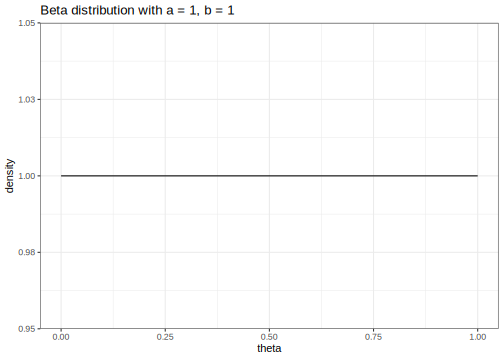
\includegraphics[width=0.48\linewidth]{bookdown_files/figure-latex/betas2-1} 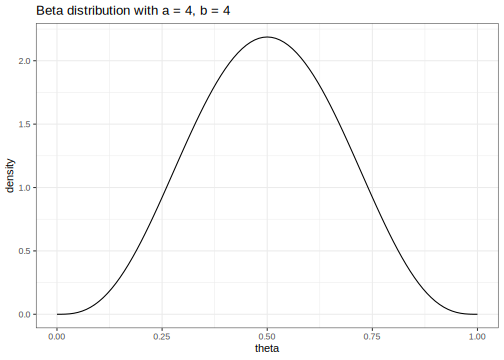
\includegraphics[width=0.48\linewidth]{bookdown_files/figure-latex/betas2-2} 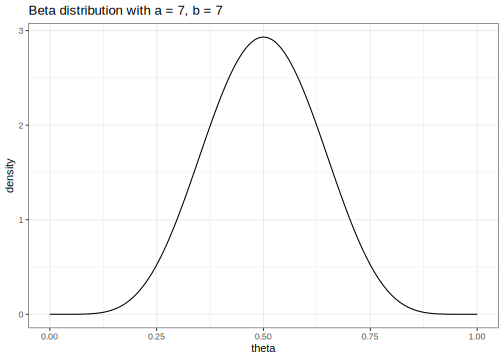
\includegraphics[width=0.48\linewidth]{bookdown_files/figure-latex/betas2-3} 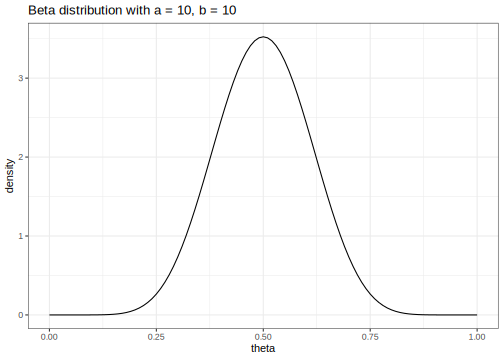
\includegraphics[width=0.48\linewidth]{bookdown_files/figure-latex/betas2-4} 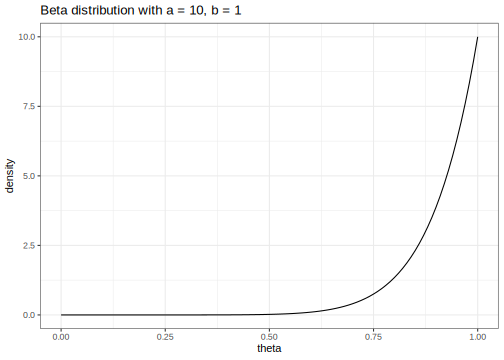
\includegraphics[width=0.48\linewidth]{bookdown_files/figure-latex/betas2-5} 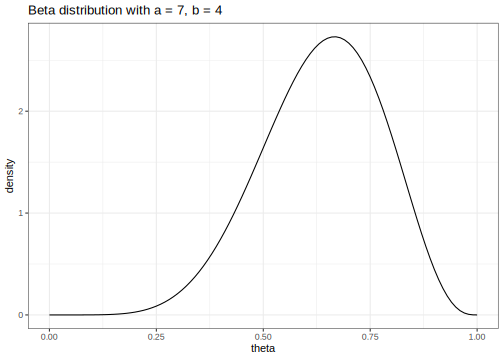
\includegraphics[width=0.48\linewidth]{bookdown_files/figure-latex/betas2-6} 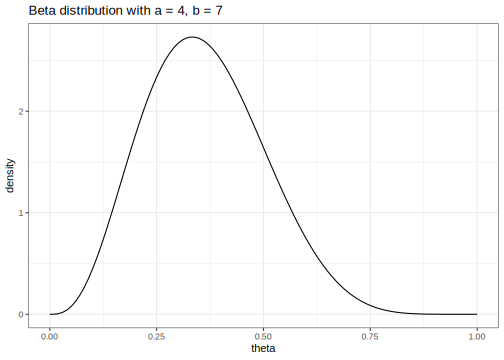
\includegraphics[width=0.48\linewidth]{bookdown_files/figure-latex/betas2-7} 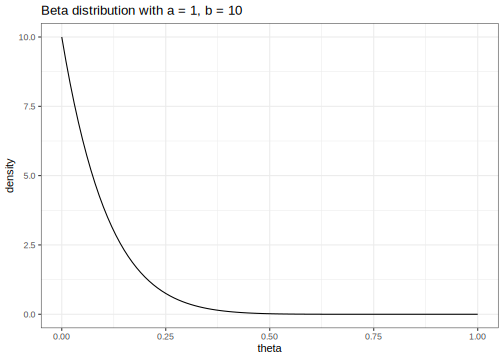
\includegraphics[width=0.48\linewidth]{bookdown_files/figure-latex/betas2-8} \caption{Examples of Beta distributions with different parameters.}\label{fig:betas2}
\end{figure}

As in the Binomial and Normal distributions that we saw in chapter 1, one can analytically derive the formulas for the expectation and variance of the Beta distribution. These are:

\begin{equation}
\operatorname{E}[X] = \frac{a}{a+b} \quad \operatorname{var}(X)=\frac {a \cdot b }{(a + b )^{2}(a + b +1)}
\label{eq:meanvar}
\end{equation}

As an example, choosing \(a=4\) and \(b=4\) would mean that the answer ``umbrella'' is as likely as a different answer, but we are relatively unsure about this. We could express our uncertainty by computing the region over which we are 95\% certain that the value of the parameter lies; this is the \textbf{95\% credible interval}. For this, we would use the \texttt{qbeta} function in R; the parameters \(a\) and \(b\) are called \texttt{shape1} and \texttt{shape2} in \texttt{R}.

\begin{Shaded}
\begin{Highlighting}[]
\KeywordTok{qbeta}\NormalTok{(}\KeywordTok{c}\NormalTok{(}\FloatTok{0.025}\NormalTok{,}\FloatTok{0.975}\NormalTok{),}\DataTypeTok{shape1=}\DecValTok{4}\NormalTok{,}\DataTypeTok{shape2=}\DecValTok{4}\NormalTok{)}
\end{Highlighting}
\end{Shaded}

\begin{verbatim}
## [1] 0.18 0.82
\end{verbatim}

If we were to choose \(a=10\) and \(b=10\), we would still be assuming that a priori the answer ``umbrella'' is just as likely as some other answer, but now our prior uncertainty about this mean is lower, as the 95\% credible interval computed below shows.

\begin{Shaded}
\begin{Highlighting}[]
\KeywordTok{qbeta}\NormalTok{(}\KeywordTok{c}\NormalTok{(}\FloatTok{0.025}\NormalTok{,}\FloatTok{0.975}\NormalTok{),}\DataTypeTok{shape1=}\DecValTok{10}\NormalTok{,}\DataTypeTok{shape2=}\DecValTok{10}\NormalTok{)}
\end{Highlighting}
\end{Shaded}

\begin{verbatim}
## [1] 0.29 0.71
\end{verbatim}

In Figure \ref{fig:betas2}, we can see also the difference in uncertainty in these two examples graphically.

Which prior should we choose? In a real data analysis problem, the choice of prior would depend on what prior knowledge we want to bring into the analysis. If we don't have much prior information, we could use \(a=b=1\); this gives us a uniform prior. This kind of prior goes by various names: \textbf{non-informative prior}, or \textbf{weakly informative prior}. By contrast, if we have a lot of prior knowledge and/or a strong belief (e.g., based on a particular theory's predictions, or prior data) that \(\theta\) has a particular range of plausible values, we can use a different set of a,b values to reflect our belief about the parameter. Notice in the above example that the larger our parameters a and b, the narrower the spread of the distribution; i.e., the lower our uncertainty about the mean value of the parameter.

For the moment, just for illustration, we choose the values \(a=4\) and \(b=4\) for the Beta prior. Then, our prior for \(\theta\) is the following Beta PDF:

\begin{equation}
p(\theta) = \frac{1}{B(4,4)} \theta^{3} (1-\theta)^{3}
\end{equation}

Having chosen a likelihood, and having defined a prior on \(\theta\), we are ready to carry out our first Bayesian analysis to derive a posterior distribution for \(\theta\).

\hypertarget{using-bayes-rule-to-compute-the-posterior-pthetank}{%
\subsection{\texorpdfstring{Using Bayes' rule to compute the posterior \(p(\theta|n,k)\)}{Using Bayes' rule to compute the posterior p(\textbackslash{}theta\textbar{}n,k)}}\label{using-bayes-rule-to-compute-the-posterior-pthetank}}

Having specified the likelihood and the prior, we will now use Bayes' rule to calculate \(p(\theta|n,k)\). Using Bayes' rule simply involves replacing the Likelihood and the Prior we defined above into the equation we saw earlier:

\begin{equation}
\hbox{Posterior} = \frac{\hbox{Likelihood} \cdot \hbox{Prior}}{\hbox{Marginal Likelihood}}
\end{equation}

Replace the terms for likelihood and prior into this equation:

\begin{equation}
p(\theta|n=10,k=8) = \frac{\left[\binom{10}{8} \theta^8 \cdot (1-\theta)^{2}\right]  \times \left[\frac{1}{B(4,4)} \times \theta^{3} (1-\theta)^{3}\right]}{p(k=8)}
\label{eq:betaunpost}
\end{equation}

where \(p(k=8)\) is \(\int_{0}^1 p(k=8|n,\theta) p(\theta)\, d\theta\). This term will be a constant once the number of successes \(k\) is known; this is the marginal likelihood we encountered in chapter 1. In fact, once \(k\) is known, there are several constant values in the above equation; they are constants because none of them depend on the parameter of interest, \(\theta\). We can collect all of these together:

\begin{equation}
p(\theta|n=10,k=8) =   \left[ \frac{\binom{10}{8}}{B(4,4)\times p(k=8)} \right]   [\theta^8 (1-\theta)^{2} \times  \theta^{3} (1-\theta)^{3}]
\label{eq:betaunpost2}
\end{equation}

The first term that is in square brackets, \(\frac{\binom{10}{8}}{B(4,4)\times p(y)}\), is all the constants collected together, and is the normalizing constant we have seen before; it makes the posterior distribution \(p(\theta|n=10,k=8)\) sum to one. Since it is a constant, we can ignore it for now and focus on the two other terms in the equation. Because we are ignoring the constant, we will now say that the posterior is proportional to the right-hand side.

\BeginKnitrBlock{rmdnote}
to-do: introduce the idea of an unnormalized posterior here? see other suggestion elsewhere.
\EndKnitrBlock{rmdnote}

\begin{equation}
p(\theta|n=10,k=8) \propto   [\theta^8 (1-\theta)^{2} \times \theta^{3} (1-\theta)^{3} ]
\label{eq:betaunpost3}
\end{equation}

A common way of writing the above equation is:

\begin{equation}
\hbox{Posterior} \propto \hbox{Likelihood} \times \hbox{Prior}
\end{equation}

Resolving the right-hand side now simply involves adding up the exponents! In this example, computing the posterior really does boil down to this simple addition operation on the exponents.

\begin{equation}
p(\theta|n=10,k=8) \propto   [\theta^{8+3} (1-\theta)^{2+3}] = \theta^{11} (1-\theta)^{5}
\label{eq:betaunpost4}
\end{equation}

The expression on the right-hand side corresponds to a Beta distribution with parameters \(a=12\), and \(b=6\). This becomes evidence if we rewrite the right-hand side such that it represents the core part of a Beta PDF. All that is missing is a normalizing constant which would make the area under the curve sum to one.

\begin{equation}
\theta^{11} (1-\theta)^{5} = \theta^{12-1} (1-\theta)^{6-1} 
\end{equation}

This core part of any PDF or PMF is called the kernel of that distribution. Without a normalizing constant, the area under the curve will not sum to one. Let's check this:

\begin{Shaded}
\begin{Highlighting}[]
\NormalTok{PostFun<-}\ControlFlowTok{function}\NormalTok{(theta)\{}
\NormalTok{  theta}\OperatorTok{^}\DecValTok{11} \OperatorTok{*}\StringTok{ }\NormalTok{(}\DecValTok{1}\OperatorTok{-}\NormalTok{theta)}\OperatorTok{^}\DecValTok{5}
\NormalTok{\}}
\NormalTok{(AUC<-}\KeywordTok{integrate}\NormalTok{(PostFun,}\DataTypeTok{lower=}\DecValTok{0}\NormalTok{,}\DataTypeTok{upper=}\DecValTok{1}\NormalTok{)}\OperatorTok{$}\NormalTok{value)}
\end{Highlighting}
\end{Shaded}

\begin{verbatim}
## [1] 0.000013
\end{verbatim}

So the area under the curve (AUC) is not 1---the posterior that we computed above is not a proper probability distribution.

All that is needed to make this into a proper probability distribution is to include a normalizing constant, which, according to the definition of the Beta distribution, would be \(B(12,6)\). This term is in fact the integral we computed above.

\begin{equation}
p(\theta|n=10,k=8) = \frac{1}{B(12,6)} \theta^{12-1} (1-\theta)^{6-1} 
\end{equation}

Now, this function will sum to one:

\begin{Shaded}
\begin{Highlighting}[]
\NormalTok{PostFun<-}\ControlFlowTok{function}\NormalTok{(theta)\{}
\NormalTok{  theta}\OperatorTok{^}\DecValTok{11} \OperatorTok{*}\StringTok{ }\NormalTok{(}\DecValTok{1}\OperatorTok{-}\NormalTok{theta)}\OperatorTok{^}\DecValTok{5}\OperatorTok{/}\NormalTok{AUC}
\NormalTok{\}}
\KeywordTok{round}\NormalTok{(}\KeywordTok{integrate}\NormalTok{(PostFun,}\DataTypeTok{lower=}\DecValTok{0}\NormalTok{,}\DataTypeTok{upper=}\DecValTok{1}\NormalTok{)}\OperatorTok{$}\NormalTok{value,}\DecValTok{2}\NormalTok{)}
\end{Highlighting}
\end{Shaded}

\begin{verbatim}
## [1] 1
\end{verbatim}

\hypertarget{summary-of-the-procedure}{%
\subsection{Summary of the procedure}\label{summary-of-the-procedure}}

To summarize, we started with a Binomial likelihood, multiplied it with the prior \(\theta \sim Beta(4,4)\), and obtained the posterior \(p(\theta|n,k) \sim Beta(12,6)\). The constants were ignored when carrying out the multiplication; we say that we computed the posterior \textbf{up to proportionality}. Finally, we showed how, in this simple example, the posterior can be rescaled to become a probability distribution, by including a proportionality constant.

The above example is a case of a \textbf{conjugate} analysis: the posterior on the parameter has the same form as the prior. The above combination of likelihood and prior is called the Beta-Binomial conjugate case. There are several other such combinations of Likelihoods and Priors that yield a posterior that has the same PDF as the prior on the parameter; some examples will appear in the exercises.

Formally, conjugacy is defined as follows:

\begin{quote}
DEFINITION
Given the likelihood \(p(y| \theta)\), if the prior \(p(\theta)\) results in a posterior \(y(\theta|y)\) that has the same form as \(p(\theta)\), then we call \(p(\theta)\) a conjugate prior.
\end{quote}

For the Beta-Binomial case, we can derive a very general relationship between the likelihood, prior, and posterior. Given the Binomial likelihood up to proportionality (ignoring the constant) \(\theta^k (1-\theta)^{n-k}\), and given the prior, also up to proportionality, \(\theta^{a-1} (1-\theta)^{b-1}\), their product will be:

\begin{equation}
\theta^k (1-\theta)^{n-k} \theta^{a-1} (1-\theta)^{b-1} = \theta^{a+k-1} (1-\theta)^{b+n-k-1} 
\end{equation}

Thus, given a \(Binomial(n,k|\theta)\) likelihood, and a \(Beta(a,b)\) prior on \(\theta\), the posterior will be \(Beta(a+k,b+n-k)\).

\hypertarget{visualizing-the-prior-likelihood-and-the-posterior}{%
\subsection{Visualizing the prior, likelihood, and the posterior}\label{visualizing-the-prior-likelihood-and-the-posterior}}

We established in the example above that the posterior is a Beta distribution with parameters \(a=12\), and \(b = 6\). We visualize the likelihood, prior, and the posterior alongside each other in \ref{fig:postbeta-viz}.

\begin{figure}
\centering
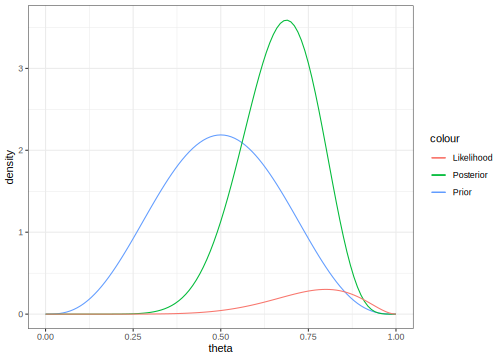
\includegraphics{bookdown_files/figure-latex/postbeta-viz-1.pdf}
\caption{\label{fig:postbeta-viz}The likelihood, prior, and posterior in the Beta-Binomial example.}
\end{figure}

We can summarize the posterior distribution either graphically as we did above, or summarize it by computing the mean and the variance. The mean gives us an estimate of the Cloze probability of producing ``umbrella'' in that sentence (given the model, i.e., given the likelihood and prior):

\begin{equation}
\operatorname{E}[\hat\theta] = \frac{12}{12+6}=0.67
\label{eq:meanPb}
\end{equation}

\begin{equation}
\operatorname{var}[\hat\theta]=\frac {12 \cdot 6 }{(12 + 6 )^{2}(12 + 6 +1)}= .01
\label{eq:varPb}
\end{equation}

We could also display the 95\% credible interval, the range over which we are 95\% certain the true value of \(\theta\) lies, given the data and model.

\begin{Shaded}
\begin{Highlighting}[]
\KeywordTok{qbeta}\NormalTok{(}\KeywordTok{c}\NormalTok{(}\FloatTok{0.025}\NormalTok{,}\FloatTok{0.975}\NormalTok{),}\DataTypeTok{shape1=}\DecValTok{12}\NormalTok{,}\DataTypeTok{shape2=}\DecValTok{6}\NormalTok{)}
\end{Highlighting}
\end{Shaded}

\begin{verbatim}
## [1] 0.44 0.86
\end{verbatim}

Typically, we would summarize the results of a Bayesian analysis by displaying the posterior distribution of the parameter (or parameters) graphically, along with the above summary statistics: the mean, the standard deviation or variance, and the 95\% credible interval. You will see many examples of such summaries later.

\hypertarget{the-posterior-distribution-is-a-compromise-between-the-prior-and-the-likelihood}{%
\subsection{The posterior distribution is a compromise between the prior and the likelihood}\label{the-posterior-distribution-is-a-compromise-between-the-prior-and-the-likelihood}}

Just for the sake of illustration, let's take four different Beta priors, each reflecting increasing certainty.

\begin{itemize}
\tightlist
\item
  Beta(a=2,b=2)
\item
  Beta(a=3,b=3)
\item
  Beta(a=6,b=6)
\item
  Beta(a=21,b=21)
\end{itemize}

Each prior reflects a belief that \(\theta=0.5\), with varying degrees of (un)certainty. Given the general formula we developed above for the Beta-Binomial case, we just need to plug in the likelihood and the prior to get the posterior:

\begin{equation}
p(\theta | n,k) \propto p(k |n,\theta) p(\theta)
\end{equation}

The four corresponding posterior distributios would be:

\begin{equation}
p(\theta\mid y,n) \propto [\theta^{8} (1-\theta)^{2}] [\theta^{2-1}(1-\theta)^{2-1}] = \theta^{10-1} (1-\theta)^{4-1}
\end{equation}

\begin{equation}
p(\theta\mid y,n) \propto [\theta^{8} (1-\theta)^{2}] [\theta^{3-1}(1-\theta)^{3-1}] = \theta^{11-1} (1-\theta)^{5-1}
\end{equation}

\begin{equation}
p(\theta\mid y,n) \propto [\theta^{8} (1-\theta)^{2}] [\theta^{6-1}(1-\theta)^{6-1}] = \theta^{14-1} (1-\theta)^{8-1}
\end{equation}

\begin{equation}
p(\theta\mid y,n) \propto [\theta^{8} (1-\theta)^{2}] [\theta^{21-1}(1-\theta)^{21-1}] = \theta^{31-1} (1-\theta)^{23-1}
\end{equation}

We can easily visualize each of these triplets of priors, likelihoods and posteriors. Use the Shiny app embedded below to visualize these different prior-likelihood combinations and look at the posterior in each case.

\BeginKnitrBlock{rmdnote}
to-do: put in a shiny app that varies the a,b parameters and the amount of data, to show how the posterior is influenced by the data and the prior under different scenarios.
\EndKnitrBlock{rmdnote}

\begin{Shaded}
\begin{Highlighting}[]
\NormalTok{knitr}\OperatorTok{::}\KeywordTok{include_app}\NormalTok{(}\StringTok{"https://vasishth.shinyapps.io/AppTypeIPower"}\NormalTok{, }
  \DataTypeTok{height =} \StringTok{"500px"}\NormalTok{)}
\end{Highlighting}
\end{Shaded}

\begin{verbatim}
## PhantomJS not found. You can install it with webshot::install_phantomjs(). If it is installed, please make sure the phantomjs executable can be found via the PATH variable.
\end{verbatim}

If you vary the prior's certainty (held constant at \(n=10, k=8\) in the above example), the posterior orients itself increasingly towards the prior. In general, we can say the following about the likelihood-prior-posterior relationship:

\begin{itemize}
\tightlist
\item
  The posterior distribution is a compromise between the prior and the likelihood.
\item
  For a given set of data, the greater the certainty in the prior, the more heavily the posterior will be influenced by the prior mean.
\item
  Conversely, for a given set of data, the greater the \textbf{un}certainty in the prior, the more heavily the posterior will be influenced by the likelihood.
\end{itemize}

Another important observation emerges if we increase the sample size from \(10\) to, say, \(1,000,000\). Suppose we still get a sample mean of \(0.8\) here, so that \(k=800,000\). Now, the posterior mean will be influenced almost entirely by the sample mean. This is because, in the general form for the posterior \(Beta(a+k,b+n-k)\) that we computed above, the \(n\) and \(k\) become very large relative to the a, b values, and dominate in determining the posterior mean.

Whenever we do a Bayesian analysis, it is good practice to check whether the parameter you are interested in estimating is sensitive to the prior specification. Such an investigation is called a \textbf{sensitivity analysis}. Later in this book, we will see many examples of sensitivity analyses in realistic data-analysis settings.

\hypertarget{incremental-knowledge-gain-using-prior-knowledge}{%
\subsection{Incremental knowledge gain using prior knowledge}\label{incremental-knowledge-gain-using-prior-knowledge}}

In the above example, we used an artificial example where we asked \(10\) participants to complete the sentence shown at the beginning of the chapter, and then we counted the number of times that they produced ``umbrella'' vs.~some other word as a continuation. Given 8 instances of ``umbrella'', and using a \(Beta(4,4)\) prior, we derived the posterior to be \(Beta(12,6)\). We could now use this posterior as our prior for the next study. Suppose that we were to carry out a second experiment, again with 10 participants, and this time \(6\) produced ``umbrella''. We could now use our new prior (Beta(12,6)) to obtain an updated posterior. We have \(a=12, b=6, n=10, k=6\). This gives us as posterior:
\(Beta(a+k,b+n-k) = Beta(12+6,6+10-6)=Beta(18,10)\).

Now, if we were to pool all our data from the 20 participants that we have now, then we would have had as data \(n=20, k=14\). Suppose that we keep our initial prior of \(a=4,b=4\). Then, our posterior would be \(Beta(4+14,4+20-14)=Beta(18,10)\). This is exactly the same posterior that we got when first analyzed the first \(10\) participants' data, derived the posterior, and then used that posterior as a prior for the next \(10\) participants' data.

This toy example illustrates an important point that has great practical important for cognitive science. One can incrementally gain information about a research question by using information from previous studies and deriving a posterior, and then use that posterior as a prior. For practical examples from psycholinguistics showing how information can be pooled from previous studies, see \citet{JaegerEngelmannVasishth2017} and \citet{NicenboimRoettgeretal}. \citet{VasishthEngelmann2020} illustrates an example of how the posterior from a previous study or collection of studies can be used to compute the posterior derived from new data. We return to this point in later chapters.

\BeginKnitrBlock{rmdnote}
to-do: check that we do.
\EndKnitrBlock{rmdnote}

\hypertarget{summary-of-concepts-introduced-in-this-chapter-1}{%
\section{Summary of concepts introduced in this chapter}\label{summary-of-concepts-introduced-in-this-chapter-1}}

In this chapter, we learnt how to use Bayes' rule in the specific case of a Binomial likelihood, and a Beta prior on the \(\theta\) parameter in the likelihood function. Our goal in any Bayesian analysis will follow the path we took in this simple example: decide on an appropriate likelihood function, decide on priors for all the parameters involved in the likelihood function, and using this model (i.e., the likelihood and the priors) derive the posterior distribution of each parameter. Then we draw inferences about our research question based on the posterior distribution of the parameter.

In the example discussed in this chapter, Bayesian analysis was easy. This was because we considered the simple conjugate case of the Beta-Binomial. In realistic data-analysis settings, our likelihood function will be very complex, and many parameters will be involved. Multiplying the likelihood function and the priors will become mathematically difficult or impossible. For such situations, we use computational methods to obtain samples from the posterior distributions of the parameters.

\BeginKnitrBlock{rmdnote}
to-do: add summary
\EndKnitrBlock{rmdnote}

\hypertarget{further-reading-1}{%
\section{Further reading}\label{further-reading-1}}

\hypertarget{exercises-1}{%
\section{Exercises}\label{exercises-1}}

\hypertarget{deriving-bayes-rule}{%
\subsection{Deriving Bayes' rule}\label{deriving-bayes-rule}}

Let A and B be two observable events. P(A) is the probability that A occurs, and P(B) is the probability that B occurs. \(P(A|B)\) is the conditional probability that A occurs given that B has happened. \(P(A,B)\) is the joint probability of A and B both occurring.

You are given the definition of conditional probability:

\begin{equation}
P(A|B)= \frac{P(A,B)}{P(B)} \hbox{ where } P(B)>0
\end{equation}

Using the above definition, and using the fact that \(P(A,B)=P(B,A)\) (i.e., the probability of A and B both occurring is the same as the probability of B and A both occurring),
derive an expression for \(P(B|A)\). Show the steps clearly in the derivation.

\hypertarget{conjugate-forms-1}{%
\subsection{Conjugate forms 1}\label{conjugate-forms-1}}

\hypertarget{computing-the-general-form-of-a-pdf-for-a-posterior}{%
\subsubsection{Computing the general form of a PDF for a posterior}\label{computing-the-general-form-of-a-pdf-for-a-posterior}}

Suppose you are given data \(k\) consisting of the number of successes, coming from a \(Binomial(n,\theta)\) distribution. Example data are shown below, generated with probability of success \(\theta=0.5\), just for illustration:

\begin{Shaded}
\begin{Highlighting}[]
\CommentTok{## data:}
\NormalTok{k<-}\KeywordTok{rbinom}\NormalTok{(}\DataTypeTok{n=}\DecValTok{1}\NormalTok{,}\DataTypeTok{size=}\DecValTok{10}\NormalTok{,}\DataTypeTok{prob=}\FloatTok{0.5}\NormalTok{)}
\NormalTok{k}
\end{Highlighting}
\end{Shaded}

\begin{verbatim}
## [1] 5
\end{verbatim}

Here, \(n\) represents the number of trials, and \(k\) the number of successes. The above code and output is just an example, and is no longer relevant for the question below.

Given \(k\) successes in n trials coming from a Binomial distribution, we define a \(Beta(a,b)\) prior on the parameter \(\theta\).

Write down the Beta distribution that represents the posterior, in terms of \(a,b, n, and k\).

\hypertarget{practical-application}{%
\subsubsection{Practical application}\label{practical-application}}

We ask 10 yes/no questions from a participant, and the participant returns 0 correct answers. We assume a Binomial likelihood function for these data. Also assume a Beta(1,1) prior on the parameter \(\theta\), which represents the probability of success. Use the result you derived above to write down the posterior distribution of the \(\theta\) parameter.

\hypertarget{conjugate-forms-2}{%
\subsection{Conjugate forms 2}\label{conjugate-forms-2}}

Suppose you have \(n\) independent and identically distributed data points from a distribution that has
the likelihood function \(f(x|\theta)=\theta(1-\theta)^{\sum_{i=1}^n x_i}\),
where the data points \(x\) can have values 0,1,2,\dots. Let the prior on \(\theta\) be Beta(a,b), a Beta distribution with parameters a,b.
The posterior distribution is a Beta distribution with parameters a* and b*.
Determine these parameters in terms of \(a\), \(b\), and \(\sum_{i=1}^n x_i\).

\hypertarget{conjugate-forms-3}{%
\subsection{Conjugate forms 3}\label{conjugate-forms-3}}

The Gamma distribution is defined in terms of the parameters a, b: Ga(a,b). The probability density function is:

\begin{equation}
Ga(a,b)=\frac{b^a \lambda^{a-1} \exp\{-b\lambda\}}{\Gamma(a)}
\end{equation}

We have data \(x_1,\dots, x_n\), with sample size \(n\) that is exponentially distributed. The exponential likelihood function is:

\begin{equation}
p(x_1,\dots,x_n | \lambda)=\lambda^n \exp \{-\lambda \sum_{i=1}^n x_i \}
\end{equation}

It turns out that if we assume a Ga(a,b) prior distribution and the above likelihood, the posterior distribution is a Gamma distribution. Find the parameters \(a'\) and \(b'\) of the posterior distribution.

\hypertarget{conjugate-forms-4}{%
\subsection{Conjugate forms 4}\label{conjugate-forms-4}}

\hypertarget{a.-computing-the-posterior}{%
\subsubsection{a. Computing the posterior}\label{a.-computing-the-posterior}}

This is a contrived example. Suppose we are modeling the number of times that a speaker says the word ``I'' per day. This could be of interest if we are studying, for example, how self-oriented a speaker is. The number of times \(x\) that the word is uttered in over a oarticular time period (here, one day) can be modeled by a Poisson distribution:

\begin{equation}
f(x\mid \theta) = \frac{\exp(-\theta) \theta^x}{x!}
\end{equation}

where the rate \(\theta\) is unknown, and the numbers of utterances of the target word on each day are independent given \(\theta\).

We are told that the prior mean of \(\theta\) is 100 and prior variance for \(\theta\) is 225. This information is based on the results of previous studies on the topic. We will use the Gamma(a,b) density (see previous question) as a prior for \(\theta\) because this is a conjugate prior to the Poisson distribution.

\begin{itemize}
\tightlist
\item
  First, visualize the prior. a Gamma density prior for \(\theta\) based on the above information.
\end{itemize}

{[}Hint: Note that we know that for a Gamma density with parameters a, b, the mean is \(\frac{a}{b}\) and the variance is \(\frac{a}{b^2}\). Since we are given values for the mean and variance, we can solve for a,b, which gives us the Gamma density.{]}

\begin{Shaded}
\begin{Highlighting}[]
\NormalTok{x<-}\DecValTok{0}\OperatorTok{:}\DecValTok{200}
\KeywordTok{plot}\NormalTok{(x,}\KeywordTok{dgamma}\NormalTok{(x,}\DecValTok{10000}\OperatorTok{/}\DecValTok{225}\NormalTok{,}\DecValTok{100}\OperatorTok{/}\DecValTok{225}\NormalTok{),}\DataTypeTok{type=}\StringTok{"l"}\NormalTok{,}\DataTypeTok{lty=}\DecValTok{1}\NormalTok{,}
     \DataTypeTok{main=}\StringTok{"Gamma prior"}\NormalTok{,}\DataTypeTok{ylab=}\StringTok{"density"}\NormalTok{,}
     \DataTypeTok{cex.lab=}\DecValTok{2}\NormalTok{,}\DataTypeTok{cex.main=}\DecValTok{2}\NormalTok{,}\DataTypeTok{cex.axis=}\DecValTok{2}\NormalTok{)}
\end{Highlighting}
\end{Shaded}

\begin{itemize}
\tightlist
\item
  Next, derive the posterior distribution of the parameter \(\theta\) up to proportionality, and write down the posterior distribution in terms of the parameters of a Gamma distribution.
\end{itemize}

\hypertarget{b.-practical-application}{%
\subsubsection{b. Practical application}\label{b.-practical-application}}

Suppose we know that the number of ``I'' utterances from a particular individual is \(115, 97, 79, 131\). Use the result you derived above to obtain the posterior distribution. In other words, write down the a,b parameters of the Gamma distribution representing the posterior distribution of \(\theta\).

Plot the prior, likelihood, and the posterior alongside each other.

Now suppose you get one new data point: 200. Write down the updated posterior (the a,b parameters of the Gamma distribution) given this new data-point. Add the updated posterior to the plot you made above.

\hypertarget{computational-bayesian-data-analysis}{%
\chapter{Computational Bayesian data analysis}\label{computational-bayesian-data-analysis}}

In the previous chapter, we learned how to analytically derive the posterior distribution of the parameters in our model.
In practice, however, this is possible for only a very limited number of cases. Although the numerator of the Bayes rule, the unnormalized posterior, is easy to calculate (by multiplying the probability density/mass functions analytically), the denominator, the marginal likelihood, requires us to integrate the numerator; see \eqref{eq:bayesbrms}.

\begin{equation}
\begin{aligned}
p(\Theta|y) &= \cfrac{ p(y|\Theta) \cdot p(\Theta) }{p(y)}\\
p(\Theta|y) &= \cfrac{ p(y|\Theta) \cdot p(\Theta) }{\int_{\Theta} p(y|\Theta) \cdot p(\Theta) d\Theta }
\end{aligned}
\label{eq:bayesbrms}
\end{equation}

Unless we are dealing with conjugate distributions, the solution will be extremely hard to derive or there will be no analytical solution. This was the major bottleneck of Bayesian analysis in the past, and required Bayesian practitioners to program an approximation method by themselves before they could even begin the Bayesian analysis. Fortunately, many of the probabilistic programming languages freely available today (see the next section for a listing) allow us to define our models without having to acquire expert knowledge about the relevant numerical techniques.

\hypertarget{deriving-the-posterior-through-sampling}{%
\section{Deriving the posterior through sampling}\label{deriving-the-posterior-through-sampling}}

Let's say that we want to derive the posterior of the model from \ref{sec:analytical}, that is, the posterior distribution of the Cloze probability of \emph{``umbrella''}, \(\theta\), given the following data: a word (e.g., \emph{``umbrella''}) was answered 80 out of 100 times, and assuming a binomial distribution as the likelihood function, and \(Beta(a=4,b=4)\) as a prior distribution for the Cloze probability. If we have samples from the posterior distribution of \(\theta\), instead of an analytically derived posterior distribution, given enough samples we will have a good approximation of the real posterior distribution. Getting samples from the posterior will be the only viable option in the models that we will discuss in this book. By ``getting samples'', we are talking about a situation analogous to when we use \texttt{rbinom} or \texttt{rnorm} to obtain samples from a particular distribution.

Thanks to probabilistic programming languages, it will be relatively straightforward to get these samples, and we will discuss how we will do it in more detail in the next section. But for now let's assume that we used Stan, \texttt{brms}, or even our hand-made sampler, and we got 20000 samples from the posterior distribution of the Cloze probability, \(\theta\): 0.793, 0.776, 0.726, 0.685, 0.776, 0.801, 0.722, 0.78, 0.739, 0.802, 0.809, 0.736, 0.78, 0.793, 0.835, 0.791, 0.773, 0.744, 0.816, 0.807, \ldots{} Figure \ref{fig:betapost} shows that the approximation of the posterior looks quite similar to the real posterior. And in fact the difference between the true and the approximated mean and variance are -0.0001 and -0.00002 respectively.



\begin{figure}
\centering
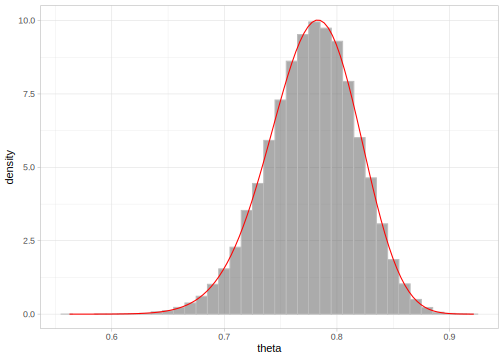
\includegraphics{bookdown_files/figure-latex/betapost-1.pdf}
\caption{\label{fig:betapost}Histogram of the samples of \(\theta\) from the posterior distribution calculated through sampling in gray; density plot of the exact posterior in red.}
\end{figure}

\hypertarget{bayesian-regression-models-using-stan-brms}{%
\subsection{Bayesian Regression Models using `Stan': brms}\label{bayesian-regression-models-using-stan-brms}}

The surge in popularity of Bayesian statistics is closely tied to the increase in computing power and the appearance of probabilistic programming languages, such as WinBUGS \citep{lunn2000winbugs}, JAGS \citep{plummer2016jags}, and more recently pymc3 \citep{Salvatier2016} and Stan \citep{carpenter2017stan}. These statistical languages allow the user to define models without having to deal (for the most part) with the complexities of the sampling process. However, they require learning a new language since they the user has to fully specify the statistical model using a particular syntax.\footnote{The python package pymc3 is an exception since it is fully integrated into python.} Furthermore, some knowledge of the sampling process is needed to correctly parameterize the models and to avoid convergences issues (these topics will be covered in detail later in this book).

There are some alternatives that allow Bayesian inference in \texttt{R} without having to fully specify the model ``by hand''. The packages \texttt{rstanarm} \citep{rstanarm} and \texttt{brms} \citep{R-brms} provide Bayesian equivalents of many popular R model-fitting functions, such as (g)lmer \citep{lme4new}; both these packages use Stan for the back-end estimation and sampling.\\
JASP \citep{JASP2019} provides a graphical user interface for both frequentist and Bayesian modeling, and is intended to be an open-source alternative to SPSS.

We will focus on \texttt{brms} in the first part of the book. This is because it can be useful for a smooth transition from frequentist models to their Bayesian equivalents. Although \texttt{brms} is powerful enough to satisfy the statistical needs of many cognitive scientists, it has the added benefit that the Stan code can be inspected (with the functions \texttt{make\_stancode} and \texttt{make\_standata}), allowing the users to customize their models or learn from the code produced internally by \texttt{brms} to eventually transition to write the models entirely in Stan.

\hypertarget{sec:simplenormal}{%
\subsubsection{A simple linear model: A single participant pressing a button repeatedly}\label{sec:simplenormal}}

We'll use the following example to illustrate the basic steps for fitting a model. Let's say we have data from a participant repeatedly pressing the space bar as fast as possible, without paying attention to any stimuli. The data are reaction times in milliseconds for each word in each trial. We would like to know how long it takes to press a key when there is no decision involved.

Let's model the data with the following assumptions:

\begin{enumerate}
\def\labelenumi{\arabic{enumi}.}
\tightlist
\item
  There is a true underlying time, \(\mu\), that the participant needs to press the space bar.
\item
  There is some noise in this process.
\item
  The noise is normally distributed (this assumption is questionable given that reaction times are generally skewed; we fix this assumption later).
\end{enumerate}

This means that the likelihood for each observation \(n\) will be:

\begin{equation}
\begin{aligned}
rt_n \sim Normal(\mu, \sigma)
\end{aligned}
\label{eq:rtlik}
\end{equation}

where \(n =1 \ldots N\), and \(rt\) is the dependent variable (reaction times in milliseconds). The variable \(N\) indexes the total number of data points. The letter \(\mu\) indicates the \emph{location} of the normal distribution function, the location parameter shifts the distribution left or right on the horizontal axis. For the normal distribution, the location is also the mean of the distribution. The letter \(\sigma\) indicates the \emph{scale} of the distribution, as the scale decreases, the distribution gets narrower. The compressing approaches a spike (all the probability mass in one point) as the scale parameter goes to zero. For the normal distribution, the scale is also its standard deviation.

For a frequentist model that will give us the maximum likelihood estimate (the sample mean) of the time it takes to press the space bar, this would be enough information to write the formula in \texttt{R}, \texttt{rt\ \textasciitilde{}\ 1}, and plug it into the function \texttt{lm()} together with the data: \texttt{lm(rt\ \textasciitilde{}\ 1,\ data)}. The meaning of the \texttt{1} here is that there is no predictor associated with this parameter, and \texttt{lm} will estimate the so-called intercept of the model, in our case \(\mu\).

For a Bayesian model, we will also need to define priors for the two parameters of our model. Let's say that we know for sure that the time it takes to press a key will be positive and lower than a minute (60000ms), but we don't want to make a commitment regarding which values are more likely. We encode what we know about the noise in the task in \(\sigma\): we know that this parameter must be positive and we'll assume that any value below 2000ms is equally likely. These priors are in general strongly discouraged because even when we know very little, a flat (or very wide) prior will almost never be the best approximation of what we know. We'll use them in this section for pedagogical purposes; the next chapter will show more realistic uses of priors.

\begin{equation}
\begin{aligned}
\mu &\sim Uniform(0, 60000) \\
\sigma &\sim Uniform(0, 2000) 
\end{aligned}
\label{eq:rtpriors}
\end{equation}

We'll first load the data from \texttt{data/button\_press.csv}:

\begin{Shaded}
\begin{Highlighting}[]
\NormalTok{df_noreading_data <-}\StringTok{ }\KeywordTok{read_csv}\NormalTok{(}\StringTok{"./data/button_press.csv"}\NormalTok{)}
\NormalTok{df_noreading_data}
\end{Highlighting}
\end{Shaded}

\begin{verbatim}
## # A tibble: 361 x 2
##      rt trialn
##   <dbl>  <dbl>
## 1   141      1
## 2   138      2
## 3   128      3
## 4   132      4
## 5   126      5
## # ... with 356 more rows
\end{verbatim}

It is a good idea to look at the distribution of the data before doing anything else; see Figure \ref{fig:m1visualize}. As we suspected, the data look a bit skewed, but we ignore this for the moment.

\begin{Shaded}
\begin{Highlighting}[]
\KeywordTok{ggplot}\NormalTok{(df_noreading_data, }\KeywordTok{aes}\NormalTok{(rt)) }\OperatorTok{+}
\StringTok{  }\KeywordTok{geom_density}\NormalTok{() }\OperatorTok{+}
\StringTok{  }\KeywordTok{ggtitle}\NormalTok{(}\StringTok{"Button-press data"}\NormalTok{)}
\end{Highlighting}
\end{Shaded}

\begin{figure}
\centering
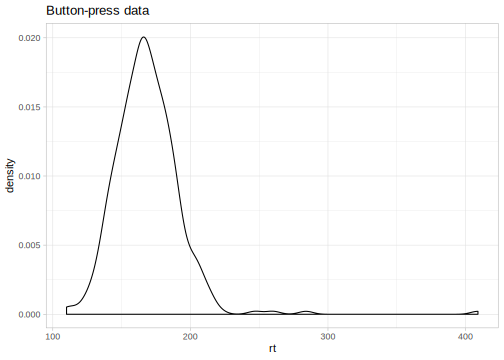
\includegraphics{bookdown_files/figure-latex/m1visualize-1.pdf}
\caption{\label{fig:m1visualize}Visualizing the data}
\end{figure}

\hypertarget{specifying-the-model-in-brms}{%
\paragraph{\texorpdfstring{Specifying the model in \texttt{brms}}{Specifying the model in brms}}\label{specifying-the-model-in-brms}}

We'll fit the model defined by equations \eqref{eq:rtlik}-\eqref{eq:rtlik} with \texttt{brms} in the following way:

\begin{Shaded}
\begin{Highlighting}[]
\NormalTok{fit_press <-}\StringTok{ }\KeywordTok{brm}\NormalTok{(rt }\OperatorTok{~}\StringTok{ }\DecValTok{1}\NormalTok{,}
  \DataTypeTok{data =}\NormalTok{ df_noreading_data,}
  \DataTypeTok{family =} \KeywordTok{gaussian}\NormalTok{(),}
  \DataTypeTok{prior =} \KeywordTok{c}\NormalTok{(}
    \KeywordTok{prior}\NormalTok{(}\KeywordTok{uniform}\NormalTok{(}\DecValTok{0}\NormalTok{, }\DecValTok{60000}\NormalTok{), }\DataTypeTok{class =}\NormalTok{ Intercept),}
    \KeywordTok{prior}\NormalTok{(}\KeywordTok{uniform}\NormalTok{(}\DecValTok{0}\NormalTok{, }\DecValTok{2000}\NormalTok{), }\DataTypeTok{class =}\NormalTok{ sigma)}
\NormalTok{  ),}
  \DataTypeTok{chains =} \DecValTok{4}\NormalTok{,}
  \DataTypeTok{iter =} \DecValTok{2000}\NormalTok{,}
  \DataTypeTok{warmup =} \DecValTok{1000}
\NormalTok{)}
\end{Highlighting}
\end{Shaded}

The \texttt{brms} code has some differences from a model fit with \texttt{lm} (or \texttt{lmer} from the \texttt{lme4} package). At this beginning stage, we'll focus on the following options:

\begin{enumerate}
\def\labelenumi{\arabic{enumi}.}
\tightlist
\item
  The term \texttt{family\ =\ gaussian()} makes explicit that the underlying likelihood function is a normal distribution (Gaussian and normal are synonyms) that is implicit in lm(er). Other linking functions are possible, exactly as in the glm(er) function.
\item
  The term \texttt{prior} takes as argument a vector of priors. Although this specification of priors is optional, the researcher should always explicitly specify each prior. Otherwise, \texttt{brms} will define a prior by default, which may or may not be appropriate for the research area.
\item
  The term \texttt{chains} refers to the number of independent runs for sampling (by default four).
\item
  The term \texttt{iter} refers to the number of iterations that the sampler makes to sample from the posterior distribution of each parameter (by default 2000).
\item
  The term \texttt{warmup} refers to the number of iterations from the start of sampling that are eventually discarded (by default half of iter).
\end{enumerate}

The last three options (together with \texttt{control} that was not used before) determine the behavior of the sampler algorithm: the No-U-Turn Sampler \citep[NUTS;][]{hoffmanNoUTurnSamplerAdaptively2014} extension of Hamiltonian Monte Carlo \citep{duaneHybridMonteCarlo1987, nealMCMCUsingHamiltonian2011}. We will discuss sampling in more depth in chapter ??, but we explain here the basic process.

\hypertarget{sampling-and-convergence-in-a-nutshell}{%
\paragraph{Sampling and convergence in a nutshell}\label{sampling-and-convergence-in-a-nutshell}}

We start four chains independent from each other. Each chain ``searches'' for samples of the posterior in a multidimensional space, where each parameter corresponds to a dimension, and the shape of this space is determined by the priors and the likelihood. The chains start in random locations and in each iteration they take one sample each. The samples at the beginning do not belong to the posterior distribution. Eventually, the chains end up in the vicinity of the posterior distribution, and from that point onwards the samples will belong to the posterior. That means that at the beginning the samples from the different chains will be far from each other, but that \emph{at some point} they will converge. While there are no guarantees that we are running the chains for enough iterations, the default values of \texttt{brms} (and Stan) are in many cases enough to achieve that, and when they are not, we will receive warnings with recommendations. If the chains converged to the same distribution, by removing the ``warmup'' (also called burn-in) samples--by default half of a total of 2000 iterations--, we make sure that we do not get samples from the path to the posterior distribution; see figure \ref{fig:warmup}. Stan runs diagnostics with the information from the chains, and if there are no warnings after fitting the model, we can be reasonable sure that the model converged and our samples are from the true posterior distribution. However, we do need to run more than one chain (preferably four), with a couple of thousands of iterations (at least) so that the diagnostics will work.



\begin{figure}
\centering
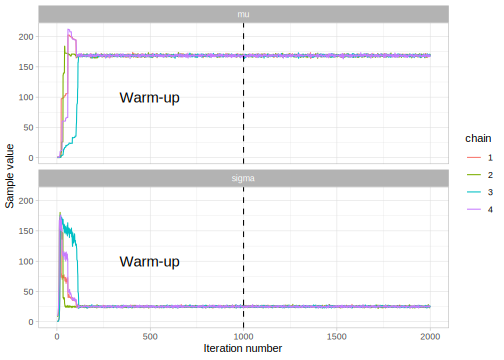
\includegraphics{bookdown_files/figure-latex/warmup-1.pdf}
\caption{\label{fig:warmup}Trace plot of the \texttt{brms} model}
\end{figure}

\hypertarget{output-of-brms}{%
\paragraph{\texorpdfstring{Output of \texttt{brms}}{Output of brms}}\label{output-of-brms}}

If the model converged (i.e., if we didn't have any warning messages), the output of the sampling process shows the samples of the posterior distributions of each of the parameters:

\begin{Shaded}
\begin{Highlighting}[]
\KeywordTok{posterior_samples}\NormalTok{(fit_press) }\OperatorTok\StringTok{ }\KeywordTok{str}\NormalTok{() }
\end{Highlighting}
\end{Shaded}

\begin{verbatim}
## 'data.frame':    4000 obs. of  3 variables:
##  $ b_Intercept: num  167 170 169 167 167 ...
##  $ sigma      : num  24.6 25.2 25.5 23.4 26.9 ...
##  $ lp__       : num  -1688 -1689 -1688 -1690 -1690 ...
\end{verbatim}

Notice that \texttt{b\_Intercept} corresponds to our \(\mu\) and that \texttt{lp} is not really part of the posterior, it's the density of the unnormalized posterior for each iteration.

We can plot the histogram and the trace plot after the warmup:

\begin{Shaded}
\begin{Highlighting}[]
\KeywordTok{plot}\NormalTok{(fit_press)}
\end{Highlighting}
\end{Shaded}

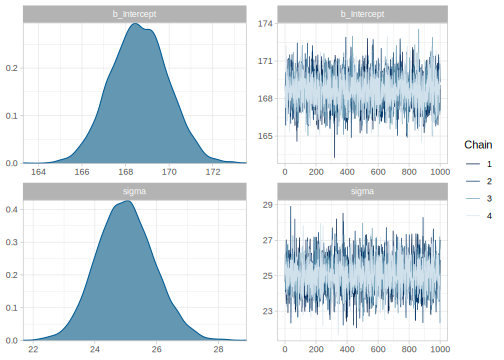
\includegraphics{bookdown_files/figure-latex/unnamed-chunk-56-1.pdf}

And \texttt{brms} provides a nice summary:

\begin{Shaded}
\begin{Highlighting}[]
\NormalTok{fit_press}
\CommentTok{# posterior_summary(fit_press) is also useful}
\end{Highlighting}
\end{Shaded}

\begin{verbatim}
##  Family: gaussian 
##   Links: mu = identity; sigma = identity 
## Formula: rt ~ 1 
##    Data: df_noreading_data (Number of observations: 361) 
## Samples: 4 chains, each with iter = 2000; warmup = 1000; thin = 1;
##          total post-warmup samples = 4000
## 
## Population-Level Effects: 
##           Estimate Est.Error l-95% CI u-95% CI Rhat
## Intercept   168.64      1.34   166.08   171.27 1.00
##           Bulk_ESS Tail_ESS
## Intercept     3648     2744
## 
## Family Specific Parameters: 
##       Estimate Est.Error l-95% CI u-95% CI Rhat
## sigma    25.01      0.94    23.17    26.90 1.00
##       Bulk_ESS Tail_ESS
## sigma     3311     2528
## 
## Samples were drawn using sampling(NUTS). For each parameter, Eff.Sample 
## is a crude measure of effective sample size, and Rhat is the potential 
## scale reduction factor on split chains (at convergence, Rhat = 1).
\end{verbatim}

Notice that the \texttt{Estimate} is just the mean of the posterior sample, and
CI are the 95\% quantiles:

\begin{Shaded}
\begin{Highlighting}[]
\KeywordTok{posterior_samples}\NormalTok{(fit_press)}\OperatorTok{$}\NormalTok{b_Intercept }\OperatorTok\StringTok{ }\KeywordTok{mean}\NormalTok{()}
\end{Highlighting}
\end{Shaded}

\begin{verbatim}
## [1] 169
\end{verbatim}

\begin{Shaded}
\begin{Highlighting}[]
\KeywordTok{posterior_samples}\NormalTok{(fit_press)}\OperatorTok{$}\NormalTok{b_Intercept }\OperatorTok\StringTok{ }\KeywordTok{quantile}\NormalTok{(}\KeywordTok{c}\NormalTok{(}\FloatTok{0.025}\NormalTok{, }\FloatTok{.975}\NormalTok{))}
\end{Highlighting}
\end{Shaded}

\begin{verbatim}
## 2.5%  98% 
##  166  171
\end{verbatim}

We see that we can fit our model without problems, and we get some
posterior distributions for our parameters. However, we should ask ourselves the following questions:

\begin{enumerate}
\def\labelenumi{\arabic{enumi}.}
\tightlist
\item
  What information are the priors encoding? Do the priors make sense?
\item
  Does the likelihood assumed in the model make sense for the data?
\end{enumerate}

We'll try to answer these questions by looking at the \emph{Prior and posterior predictive distributions}, and by doing sensitivity analyses as described in the following sections.

\hypertarget{sec:priorpred}{%
\section{Prior predictive distribution}\label{sec:priorpred}}

We had defined the following priors for our linear model:

\begin{equation}
\begin{aligned}
\mu &\sim Uniform(0, 60000) \\
\sigma &\sim Uniform(0, 2000) 
\end{aligned}
\label{eq:rtpriorsrepeated}
\end{equation}

These priors encode assumptions about the kind of data we would expect to see in a future study.
To understand these assumptions, we are going to generate data from the model; such data, which is generated entirely by the prior distributions, is called the prior predictive distribution. Generating prior predictive distributions repeatedly helps us to check whether the priors make sense. What we want to know here is, do the priors generate realistic-looking data?

Formally, we want to know the density \(p(\cdot)\) of data points \(y_{pred_1,\dots,y_pred_N}\) from a dataset \(D_{pred}\) of length \(N\), given a vector of priors \(\Theta\) and our likelihood \(p(\cdot|\Theta)\); (in our example, \(\Theta=\langle\mu,\sigma \rangle\)). Formally, the prior predictive density is written as follows:

\begin{equation}
p(D_{pred}) = p(y_{pred_1},\dots,y_{pred_n})= \int_\Theta p(y_{pred_1}|\Theta)\cdot p(y_{pred_2}|\Theta)\cdots p(y_{pred_N}|\Theta) p(\Theta) \, d\Theta 
\end{equation}

In essence, we integrate out the vector of parameters, and we end up with the probability distribution of possible datasets given the priors and the likelihood we have defined, \emph{before we encounter any observations}.

We can completely avoid doing the integration by generating samples from the prior distribution instead. Notice here that each sample is an imaginary or potential dataset.

Here is one way to generate prior predictive distributions:

Repeat the following many times:
1. Take one sample from each of the priors.
2. Plug those samples in the likelihood and generate a dataset \(y_{pred_1},\ldots,y_{pred_n}\).

We can create a function that does this:

\begin{Shaded}
\begin{Highlighting}[]
\NormalTok{normal_predictive_distribution <-}\StringTok{ }\ControlFlowTok{function}\NormalTok{(mu_samples, sigma_samples, N_obs) \{}
  \CommentTok{# empty data frame with headers:}
\NormalTok{  df_pred <-}\StringTok{ }\KeywordTok{tibble}\NormalTok{(}\DataTypeTok{trialn =} \KeywordTok{numeric}\NormalTok{(}\DecValTok{0}\NormalTok{),}
                    \DataTypeTok{rt_pred =} \KeywordTok{numeric}\NormalTok{(}\DecValTok{0}\NormalTok{),}
                    \DataTypeTok{iter =} \KeywordTok{numeric}\NormalTok{(}\DecValTok{0}\NormalTok{))}
  \CommentTok{# i iterates from 1 to the length of mu_samples,}
  \CommentTok{# which we assume is identical to }
  \CommentTok{# the length of the sigma_samples:}
  \ControlFlowTok{for}\NormalTok{ (i }\ControlFlowTok{in} \KeywordTok{seq_along}\NormalTok{(mu_samples)) \{}
\NormalTok{    mu <-}\StringTok{ }\NormalTok{mu_samples[i]}
\NormalTok{    sigma <-}\StringTok{ }\NormalTok{sigma_samples[i]}
\NormalTok{    df_pred <-}\StringTok{ }\KeywordTok{bind_rows}\NormalTok{(}
\NormalTok{      df_pred,}
      \KeywordTok{tibble}\NormalTok{(}
        \DataTypeTok{trialn =} \KeywordTok{seq_len}\NormalTok{(N_obs), }\CommentTok{#1, 2,... N_obs}
        \DataTypeTok{rt_pred =} \KeywordTok{rnorm}\NormalTok{(N_obs, mu, sigma),}
        \DataTypeTok{iter =}\NormalTok{ i}
\NormalTok{      )}
\NormalTok{    )}
\NormalTok{  \}}
\NormalTok{  df_pred}
\NormalTok{\}}
\end{Highlighting}
\end{Shaded}

The following code produces 1000 samples of the prior predictive distribution of the model that we defined in \ref{sec:simplenormal}. Although this approach works, it's quite slow (it takes about 5 seconds):

\begin{Shaded}
\begin{Highlighting}[]
\KeywordTok{tic}\NormalTok{()}
\NormalTok{N_samples <-}\StringTok{ }\DecValTok{1000}
\NormalTok{N_obs <-}\StringTok{ }\KeywordTok{nrow}\NormalTok{(df_noreading_data)}
\NormalTok{mu_samples <-}\StringTok{ }\KeywordTok{runif}\NormalTok{(N_samples, }\DecValTok{0}\NormalTok{, }\DecValTok{60000}\NormalTok{)}
\NormalTok{sigma_samples <-}\StringTok{ }\KeywordTok{runif}\NormalTok{(N_samples, }\DecValTok{0}\NormalTok{, }\DecValTok{2000}\NormalTok{)}

\KeywordTok{normal_predictive_distribution}\NormalTok{(}
  \DataTypeTok{mu_samples =}\NormalTok{ mu_samples,}
  \DataTypeTok{sigma_samples =}\NormalTok{ sigma_samples,}
  \DataTypeTok{N_obs =}\NormalTok{ N_obs}
\NormalTok{)}
\end{Highlighting}
\end{Shaded}

\begin{verbatim}
## # A tibble: 361,000 x 3
##   trialn rt_pred  iter
##    <dbl>   <dbl> <dbl>
## 1      1  37891.     1
## 2      2  38266.     1
## 3      3  38339.     1
## 4      4  38988.     1
## 5      5  39062.     1
## # ... with 3.61e+05 more rows
\end{verbatim}

\begin{Shaded}
\begin{Highlighting}[]
\KeywordTok{toc}\NormalTok{()}
\end{Highlighting}
\end{Shaded}

\begin{verbatim}
## 4.707 sec elapsed
\end{verbatim}

We can create a more efficient function in the following way. With this function, we see an approximately 10-fold increase in speed. Notice that while the distributions should be the same with both functions, the numbers that we see in the tables won't be, due to the randomness in the process of sampling.

\begin{Shaded}
\begin{Highlighting}[]
\NormalTok{normal_predictive_distribution_fast <-}\StringTok{ }\ControlFlowTok{function}\NormalTok{(mu_samples,}
\NormalTok{                                                sigma_samples,}
\NormalTok{                                                N_obs) \{}
  \CommentTok{# map_dfr works similarly to lapply, it essentially runs}
  \CommentTok{# a for-loop, and builds a dataframe with the output.}
  \CommentTok{# We iterate over the values of mu_samples and sigma_samples}
  \CommentTok{# simultaneously, and in each iteration we bind a new}
  \CommentTok{# data frame with N_obs observations.}
  \KeywordTok{map2_dfr}\NormalTok{(mu_samples, sigma_samples, }\ControlFlowTok{function}\NormalTok{(mu, sigma) \{}
    \KeywordTok{tibble}\NormalTok{(}
      \DataTypeTok{trialn =} \KeywordTok{seq_len}\NormalTok{(N_obs),}
      \DataTypeTok{rt_pred =} \KeywordTok{rnorm}\NormalTok{(N_obs, mu, sigma)}
\NormalTok{    )}
\NormalTok{  \}, }\DataTypeTok{.id =} \StringTok{"iter"}\NormalTok{) }\OperatorTok
\StringTok{    }\CommentTok{# .id is always a string and needs to be converted to a number}
\StringTok{    }\KeywordTok{mutate}\NormalTok{(}\DataTypeTok{iter =} \KeywordTok{as.numeric}\NormalTok{(iter))}
\NormalTok{\}}

\KeywordTok{tic}\NormalTok{()}
\NormalTok{(prior_pred <-}\StringTok{ }\KeywordTok{normal_predictive_distribution_fast}\NormalTok{(}
  \DataTypeTok{mu_samples =}\NormalTok{ mu_samples,}
  \DataTypeTok{sigma_samples =}\NormalTok{ sigma_samples,}
\NormalTok{  N_obs))}
\end{Highlighting}
\end{Shaded}

\begin{verbatim}
## # A tibble: 361,000 x 3
##    iter trialn rt_pred
##   <dbl>  <int>   <dbl>
## 1     1      1  36807.
## 2     1      2  37132.
## 3     1      3  38655.
## 4     1      4  39613.
## 5     1      5  39348.
## # ... with 3.61e+05 more rows
\end{verbatim}

\begin{Shaded}
\begin{Highlighting}[]
\KeywordTok{toc}\NormalTok{()}
\end{Highlighting}
\end{Shaded}

\begin{verbatim}
## 0.358 sec elapsed
\end{verbatim}

Figure \ref{fig:priorpred-simple} shows the first 18 samples of the prior predictive distribution. These are 18 predicted datasets.



\begin{Shaded}
\begin{Highlighting}[]
\NormalTok{prior_pred }\OperatorTok
\StringTok{  }\KeywordTok{filter}\NormalTok{(iter }\OperatorTok{<=}\StringTok{ }\DecValTok{18}\NormalTok{) }\OperatorTok
\StringTok{  }\KeywordTok{ggplot}\NormalTok{(}\KeywordTok{aes}\NormalTok{(rt_pred)) }\OperatorTok{+}
\StringTok{  }\KeywordTok{geom_histogram}\NormalTok{() }\OperatorTok{+}
\StringTok{  }\KeywordTok{facet_wrap}\NormalTok{(}\OperatorTok{~}\NormalTok{iter, }\DataTypeTok{ncol =} \DecValTok{3}\NormalTok{)}
\end{Highlighting}
\end{Shaded}

\begin{figure}
\centering
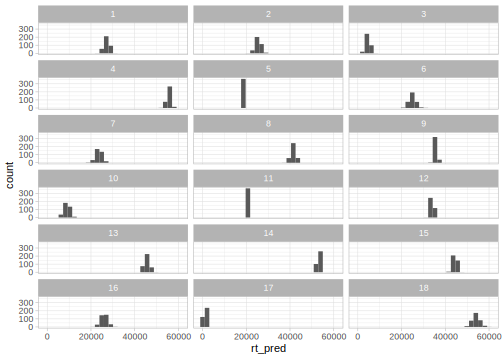
\includegraphics{bookdown_files/figure-latex/priorpred-simple-1.pdf}
\caption{\label{fig:priorpred-simple}Eighteen samples from the prior predictive distribution of the model defined in \ref{sec:simplenormal}.}
\end{figure}

The prior predictive distribution in Figure \ref{fig:priorpred-simple} shows prior datasets that are not realistic: Besides the fact that the datasets show that reaction times distributions are symmetrical--and we know that they are generally right-skewed--, some datasets present reaction times that are unrealistically long, and worst yet, dataset 18 presents negative press time values.

We can also look at the distribution of statistics here. Even if we don't know beforehand what the data should look like, it's very likely that we have some expectations for possible mean, minimum, or maximum values.



\begin{Shaded}
\begin{Highlighting}[]
\NormalTok{prior_pred }\OperatorTok
\StringTok{  }\KeywordTok{group_by}\NormalTok{(iter) }\OperatorTok
\StringTok{  }\KeywordTok{summarize}\NormalTok{(}
    \DataTypeTok{min_rt =} \KeywordTok{min}\NormalTok{(rt_pred),}
    \DataTypeTok{max_rt =} \KeywordTok{max}\NormalTok{(rt_pred),}
    \DataTypeTok{average_rt =} \KeywordTok{mean}\NormalTok{(rt_pred)}
\NormalTok{  ) }\OperatorTok
\StringTok{  }\CommentTok{# we convert the previous data frame to a long one,}
\StringTok{  }\CommentTok{# where min_rt, max_rt, average_rt are possible values}
\StringTok{  }\CommentTok{# of the columns "stat"}
\StringTok{  }\KeywordTok{pivot_longer}\NormalTok{(}\DataTypeTok{cols =} \KeywordTok{ends_with}\NormalTok{(}\StringTok{"rt"}\NormalTok{),}
               \DataTypeTok{names_to =} \StringTok{"stat"}\NormalTok{,}
               \DataTypeTok{values_to =} \StringTok{"rt"}\NormalTok{) }\OperatorTok
\StringTok{  }\KeywordTok{ggplot}\NormalTok{(}\KeywordTok{aes}\NormalTok{(rt)) }\OperatorTok{+}
\StringTok{  }\KeywordTok{geom_histogram}\NormalTok{(}\DataTypeTok{binwidth =} \DecValTok{500}\NormalTok{) }\OperatorTok{+}
\StringTok{  }\KeywordTok{facet_wrap}\NormalTok{(}\OperatorTok{~}\NormalTok{stat, }\DataTypeTok{ncol =} \DecValTok{1}\NormalTok{)}
\end{Highlighting}
\end{Shaded}

\begin{figure}
\centering
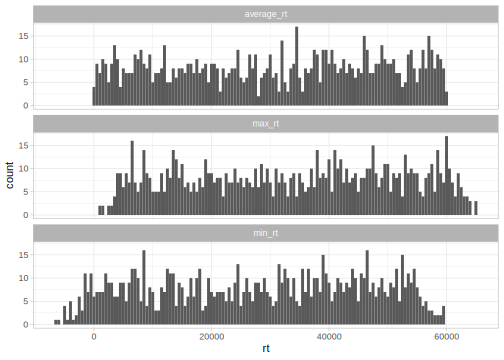
\includegraphics{bookdown_files/figure-latex/priorpred-stats-1.pdf}
\caption{\label{fig:priorpred-stats}Prior predictive distribution of averages, maximum, and minimum value of the model defined in \ref{sec:simplenormal}.}
\end{figure}

Figure \ref{fig:priorpred-stats} shows us that we used much less prior information than what we really had: Our priors were encoding the information that any mean between 0 and 60000 is expected, even though we know that a value close to 0 or to 60000 would be extremely surprising. It should be clear that this results is because we are seeing the effects of our uniform prior on \(\mu\). Similarly, maximum values are quite ``uniform'', spanning a much wider range than what we would expect. Finally, in the distribution of minimum values, we see that negative observations are predicted. This might seem surprising (our prior for \(\mu\) excluded negative values), but the reason we observe negative values is that the prior is interpreted together with the likelihood \citep{gelmanPriorCanOften2017}, and our likelihood is a normal distribution, which will allow for negative samples no matter the value of the parameter \(\mu\).

To summarize the above discussion, our priors are clearly not very realistic given what we know about reaction times for such a button pressing task. This raises the question: what priors should we have chosen? In the next section, we consider this question.

\hypertarget{sec:sensitivity}{%
\section{The influence of priors: sensitivity analysis}\label{sec:sensitivity}}

For most cases that we will encounter in this book, there are four main classes of priors that we can choose from:

\hypertarget{flat-uninformative-priors}{%
\subsection{Flat uninformative priors}\label{flat-uninformative-priors}}

One option is to choose priors that are as uninformative as possible. The idea behind this approach is to let the data ``speak for itself'' and to not bias the statistical inference with ``subjective'' priors. There are several issues with this approach: First, the prior is as subjective as the likelihood, and in fact, different choices of likelihood might have a much stronger impact on the posterior than different choices of priors. Second, uninformative priors are in general unrealistic because they give equal weight to any value, ignoring the fact that we do have some minimal information about our parameters of interest, at the very least, the order of magnitude (reaction times will be in milliseconds and not days, EEG signals some microvolts and not volts, etc). Finally, uninformative priors make the sampling slower and might lead to problems of convergence. Unless we have a large amount of data, it would be wise to avoid them. In the real data analyses we present in this book,

\hypertarget{regularizing-priors}{%
\subsection{Regularizing priors}\label{regularizing-priors}}

If we don't have much prior information, and we have enough data (what enough means here will presently become clear when we look at specific examples), it is fine to use so-called \emph{regularizing priors}. These are priors that downweight extreme values (that is, they provide regularization), they are not very informative, and mostly let the likelihood dominate in determining the posteriors. These priors are theory-neutral; that is, they do not bias the parameters to values supported by any theory. The idea behind this type of prior is to help to stabilize computation. For many applications, they perform well, but as we will see later, they tend to be problematic if we want to use Bayes factors.

\hypertarget{principled-priors}{%
\subsection{Principled priors}\label{principled-priors}}

The idea here is to have priors that encode all (or most of) the theory-neutral information that we do have. Since we generally know how our data do and do not look like, we can build priors that truly reflect the properties of potential datasets.

\hypertarget{informative-priors}{%
\subsection{Informative priors}\label{informative-priors}}

There are cases where we have a lot of prior knowledge, and not much data. In general, unless we have \emph{very} good reasons for having informative priors, we don't want our priors to have too much influence on our posterior. An example where informative priors would be important is when we are investigating a language-impaired population from which we can't get many participants.

These four options constitute a continuum. The model from section \ref{sec:simplenormal} falls between flat uninformative and regularizing priors. The priors we used were flat but they allowed for values with at least the right order of magnitude. In practical data analysis situations, we are mostly going to choose priors that fall between regularizing and principled.

\BeginKnitrBlock{rmdnote}
to-do: I guess this section could be completed. We should do a bit more justice to people advocating for uninformative priors, and also refer to this idea of uninformative priors that are invariant to transformations.
SV: I think more discussion would help beginners. We need to test this section out with readers who are complete beginners.
\EndKnitrBlock{rmdnote}

\hypertarget{revisiting-the-button-pressing-example-with-different-priors}{%
\section{Revisiting the button-pressing example with different priors}\label{revisiting-the-button-pressing-example-with-different-priors}}

\BeginKnitrBlock{rmdnote}
to-do: SV: could we show the posteriors from the last and this model side by side using ridge plots?
\EndKnitrBlock{rmdnote}

What would happen if we use even wider priors for the model defined in \ref{sec:simplenormal}? We could assume that every mean between \(-10^{10}\) and \(10^{10}\) ms is equally likely. Regarding the standard deviation, we could assume that any value between \(0\) and \(10^{10}\) is equally likely. We keep the likelihood as it is, and we encode the following priors:

\begin{equation}
\begin{aligned}
\mu &\sim Uniform(-10^{10}, 10^{10}) \\
\sigma &\sim Uniform(0,  10^{10}) 
\end{aligned}
\label{eq:rtpriorsflat}
\end{equation}

\begin{Shaded}
\begin{Highlighting}[]
\CommentTok{# We fit the model with the default setting of the sampler:}
\CommentTok{# 4 chains, 2000 iterations with half of them as warmup.}
\NormalTok{fit_press_unif <-}\StringTok{ }\KeywordTok{brm}\NormalTok{(rt }\OperatorTok{~}\StringTok{ }\DecValTok{1}\NormalTok{,}
  \DataTypeTok{data =}\NormalTok{ df_noreading_data,}
  \DataTypeTok{family =} \KeywordTok{gaussian}\NormalTok{(),}
  \DataTypeTok{prior =} \KeywordTok{c}\NormalTok{(}
    \KeywordTok{prior}\NormalTok{(}\KeywordTok{uniform}\NormalTok{(}\OperatorTok{-}\DecValTok{10}\OperatorTok{^}\DecValTok{10}\NormalTok{, }\DecValTok{10}\OperatorTok{^}\DecValTok{10}\NormalTok{), }\DataTypeTok{class =}\NormalTok{ Intercept),}
    \KeywordTok{prior}\NormalTok{(}\KeywordTok{uniform}\NormalTok{(}\DecValTok{0}\NormalTok{, }\DecValTok{10}\OperatorTok{^}\DecValTok{10}\NormalTok{), }\DataTypeTok{class =}\NormalTok{ sigma)}
\NormalTok{  )}
\NormalTok{)}
\end{Highlighting}
\end{Shaded}

Notice that even with these extremely unrealistic priors the output of the model is virtually identical!

\begin{Shaded}
\begin{Highlighting}[]
\NormalTok{fit_press_unif}
\end{Highlighting}
\end{Shaded}

\begin{verbatim}
##  Family: gaussian 
##   Links: mu = identity; sigma = identity 
## Formula: rt ~ 1 
##    Data: df_noreading_data (Number of observations: 361) 
## Samples: 4 chains, each with iter = 2000; warmup = 1000; thin = 1;
##          total post-warmup samples = 4000
## 
## Population-Level Effects: 
##           Estimate Est.Error l-95% CI u-95% CI Rhat
## Intercept   168.61      1.30   166.09   171.16 1.00
##           Bulk_ESS Tail_ESS
## Intercept     3098     2408
## 
## Family Specific Parameters: 
##       Estimate Est.Error l-95% CI u-95% CI Rhat
## sigma    25.02      0.97    23.24    26.99 1.00
##       Bulk_ESS Tail_ESS
## sigma     3336     2524
## 
## Samples were drawn using sampling(NUTS). For each parameter, Eff.Sample 
## is a crude measure of effective sample size, and Rhat is the potential 
## scale reduction factor on split chains (at convergence, Rhat = 1).
\end{verbatim}

What would happen if we had used very informative priors? We will assume that means very close to 400 ms are the most likely, and that the standard deviation of the reaction times is very close to 100. We already know that this information is clearly wrong, because we have already seen the output of some models. Notice that the \(Normal_+\) notation indicates a normal distribution truncated in zero that only allows positive values:

\begin{equation}
\begin{aligned}
\mu &\sim Normal(200, 200) \\
\sigma &\sim Normal_+(0, 500) 
\end{aligned}
\label{eq:infrtpriors}
\end{equation}

\begin{Shaded}
\begin{Highlighting}[]
\NormalTok{fit_press_inf <-}\StringTok{ }\KeywordTok{brm}\NormalTok{(rt }\OperatorTok{~}\StringTok{ }\DecValTok{1}\NormalTok{,}
  \DataTypeTok{data =}\NormalTok{ df_noreading_data,}
  \DataTypeTok{family =} \KeywordTok{gaussian}\NormalTok{(),}
  \DataTypeTok{prior =} \KeywordTok{c}\NormalTok{(}
    \KeywordTok{prior}\NormalTok{(}\KeywordTok{normal}\NormalTok{(}\DecValTok{400}\NormalTok{, }\DecValTok{10}\NormalTok{), }\DataTypeTok{class =}\NormalTok{ Intercept),}
    \CommentTok{# brms knows that SD needs to be bounded by zero:}
    \KeywordTok{prior}\NormalTok{(}\KeywordTok{normal}\NormalTok{(}\DecValTok{100}\NormalTok{, }\DecValTok{10}\NormalTok{), }\DataTypeTok{class =}\NormalTok{ sigma)}
\NormalTok{  )}
\NormalTok{)}
\end{Highlighting}
\end{Shaded}

Even in this case, the likelihood mostly dominates and the new estimates are just a couple of milliseconds away from our previous estimates:

\begin{Shaded}
\begin{Highlighting}[]
\NormalTok{fit_press_unif}
\end{Highlighting}
\end{Shaded}

\begin{verbatim}
##  Family: gaussian 
##   Links: mu = identity; sigma = identity 
## Formula: rt ~ 1 
##    Data: df_noreading_data (Number of observations: 361) 
## Samples: 4 chains, each with iter = 2000; warmup = 1000; thin = 1;
##          total post-warmup samples = 4000
## 
## Population-Level Effects: 
##           Estimate Est.Error l-95% CI u-95% CI Rhat
## Intercept   168.61      1.30   166.09   171.16 1.00
##           Bulk_ESS Tail_ESS
## Intercept     3098     2408
## 
## Family Specific Parameters: 
##       Estimate Est.Error l-95% CI u-95% CI Rhat
## sigma    25.02      0.97    23.24    26.99 1.00
##       Bulk_ESS Tail_ESS
## sigma     3336     2524
## 
## Samples were drawn using sampling(NUTS). For each parameter, Eff.Sample 
## is a crude measure of effective sample size, and Rhat is the potential 
## scale reduction factor on split chains (at convergence, Rhat = 1).
\end{verbatim}

This doesn't mean that priors never matter. When there is enough data, the likelihood will dominate in determining the posterior distributions. However, even in the cases where the likelihood dominates, more accurate priors (i.e., more consistent with our real previous belief about the data) will in general speed-up model convergence.

If we are not sure about the extent to which the posterior is influenced by our priors, we can do a \emph{sensitivity analysis}: we try different priors and either verify that the posterior doesn't change drastically, or report how the posterior is affected by some specific priors \citep[for a published example in psycholinguistics, see][]{vasishthProcessingChineseRelative2013}. We will see later in this book that \emph{sensitivity analysis} becomes crucial for reporting Bayes factors (in section ???); even in cases where the choice of priors does not affect the posterior distribution, it generally affects the Bayes factor.

\hypertarget{sec:ppd}{%
\section{Posterior predictive distribution}\label{sec:ppd}}

The prior predictive distribution is a collection of datasets generated from the model (the likelihood and the priors). After we have seen the data and obtained the posterior distributions of the parameters, we can now use the \emph{posterior distributions} to generate future data from the model. In other words, given the posterior distributions of the parameters of the model, the posterior predictive distribution shows how future data might look like.

Once we have the posterior distribution \(p(\Theta\mid y)\), we can derive the predictions based on this distribution:

\begin{equation}
p(D_{pred}\mid y ) = \int_\Theta p(D_{pred}, \Theta\mid y)\, d\Theta= \int_\Theta 
p(D_{pred}\mid \Theta,y)p(\Theta\mid y)\, d\Theta
\end{equation}

Assuming that past and future observations are conditionally independent given \(\Theta\), i.e., \(p(D_{pred}\mid \Theta,y)= p(D_{pred}\mid \Theta)\), we can write:

\begin{equation}
p(D_{pred}\mid y )=\int_\Theta p(D_{pred}\mid \Theta) p(\Theta\mid y)\, d\Theta
\end{equation}

Note that we are conditioning \(D_{pred}\) only on \(y\), we do not condition on what we don't know (\(\Theta\)); we integrate out the unknown parameters. This posterior predictive distribution is different from the frequentist approach, which gives only a predictive distribution of \(D_{pred}\) given our maximum likelihood estimate of \(\theta\) (a point value). As with the prior predictive distribution, we can avoid the integration by generating samples from the posterior predictive distribution. We can use the same function that we created before, \texttt{normal\_predictive\_distribution\_fast}, with the only difference in that instead of sampling \texttt{mu} and \texttt{sigma} from the priors, we use samples from the posterior.

\begin{Shaded}
\begin{Highlighting}[]
\NormalTok{N_obs <-}\StringTok{ }\KeywordTok{nrow}\NormalTok{(df_noreading_data)}
\NormalTok{mu_samples <-}\StringTok{ }\KeywordTok{posterior_samples}\NormalTok{(fit_press)}\OperatorTok{$}\NormalTok{b_Intercept}
\NormalTok{sigma_samples <-}\StringTok{ }\KeywordTok{posterior_samples}\NormalTok{(fit_press)}\OperatorTok{$}\NormalTok{sigma}
\KeywordTok{normal_predictive_distribution_fast}\NormalTok{(}
  \DataTypeTok{mu_samples =}\NormalTok{ mu_samples,}
  \DataTypeTok{sigma_samples =}\NormalTok{ sigma_samples,}
\NormalTok{  N_obs}
\NormalTok{)}
\end{Highlighting}
\end{Shaded}

\begin{verbatim}
## # A tibble: 1,444,000 x 3
##    iter trialn rt_pred
##   <dbl>  <int>   <dbl>
## 1     1      1    154.
## 2     1      2    170.
## 3     1      3    161.
## 4     1      4    203.
## 5     1      5    181.
## # ... with 1.444e+06 more rows
\end{verbatim}

There is a built-in function provided in \texttt{brms}, that will give us the posterior predictive distribution: \texttt{posterior\_predict(fit\_press)} provides the predicted reaction times in a matrix, with the number of samples as rows and the number of observations (data-points) as columns.

We can use the posterior predictive distribution to examine the ``descriptive adequacy'' of our models \citetext{\citealp[Chapter 6]{Gelman14}; \citealp{shiffrinSurveyModelEvaluation2008}}; these are called posterior predictive checks, and what we want to establish here is that the posterior predictive data look more or less similar to the observed data. Achieving descriptive adequacy means that the current data could have been generated by the model. While passing a test of descriptive adequacy is not strong evidence in favor of a model, a major failure in descriptive adequacy can be interpreted as strong evidence against a model \citep{shiffrinSurveyModelEvaluation2008}. Thus, posterior predictive checking is an important sanity check to assess whether the model behavior is reasonable.

In many cases, we can simply use the plot functions from \texttt{brms} and \texttt{bayesplot} that take the model as an argument for the visualization posterior predictive checks. For example, we can use \texttt{pp\_check} to investigate how well the observed distribution of reaction times fit our model based on some number (11 and 100) samples of the posterior predictive distributions; see figures \ref{fig:normalppc} and \ref{fig:normalppc2}.



\begin{Shaded}
\begin{Highlighting}[]
\KeywordTok{pp_check}\NormalTok{(fit_press, }\DataTypeTok{nsamples =} \DecValTok{11}\NormalTok{, }\DataTypeTok{type =} \StringTok{"hist"}\NormalTok{)}
\end{Highlighting}
\end{Shaded}

\begin{figure}
\centering
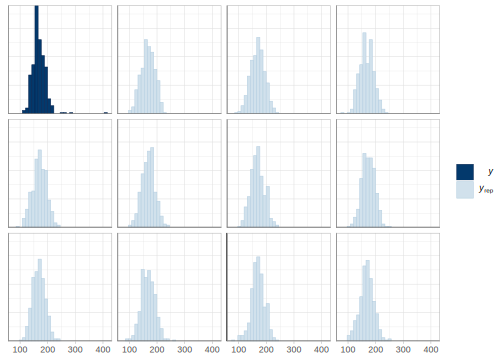
\includegraphics{bookdown_files/figure-latex/normalppc-1.pdf}
\caption{\label{fig:normalppc}Eleven samples from the posterior predictive distribution of the model \texttt{fit\_press}.}
\end{figure}



\begin{Shaded}
\begin{Highlighting}[]
\KeywordTok{pp_check}\NormalTok{(fit_press, }\DataTypeTok{nsamples =} \DecValTok{100}\NormalTok{)}
\end{Highlighting}
\end{Shaded}

\begin{figure}
\centering
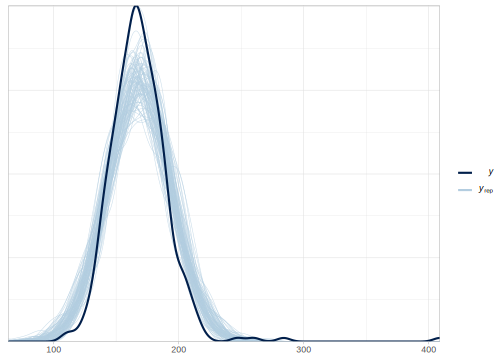
\includegraphics{bookdown_files/figure-latex/normalppc2-1.pdf}
\caption{\label{fig:normalppc2}Posterior predictive check that shows the fit of the model \texttt{fit\_press} in comparison to datasets from the posterior predictive distribution.}
\end{figure}

Notice that the real data is slightly skewed and has no values shorter than 100 ms, while the predictive distributions are centered and symmetrical; see figures \ref{fig:normalppc} and \ref{fig:normalppc2}. This posterior predictive check shows a slight mismatch between the observed and predicted data. Can we build a better model? We'll come back to this issue in the next section.

\hypertarget{comparing-different-likelihoods}{%
\subsection{Comparing different likelihoods}\label{comparing-different-likelihoods}}

Since we know that the reaction times shouldn't be normally distributed, we can choose a more realistic distribution for the likelihood. A good candidate is the log-normal distribution since a variable (such as time) that is log-normally distributed takes only positive real values and is right skewed.

\hypertarget{sec:lnfirst}{%
\subsection{The log-normal likelihood}\label{sec:lnfirst}}

If \(y\) is log-normally distributed, this means that \(\log(y)\) is normally distributed.\footnote{In fact, \(\log_e(y)\) or \(\ln(y)\), but we'll write it as just \(log()\)} Something important to notice is that the log-normal distribution is again defined using \(\mu\) and \(\sigma\), but these correspond to the mean and standard deviation of the normally distributed logarithm of the data \(y\): \(\log(y)\). Thus, when we model some data \(y\) using the log-normal likelihood, the parameters \(\mu\) and \(\sigma\) are on a different scale than the data \(y\).

We can create a log-normal distribution by exponentiating the samples of a normal distribution. See Figure \ref{fig:logndemo}.

\begin{equation}
\begin{aligned}
\log(y) &\sim Normal( \mu, \sigma)\\
y &\sim \exp(Normal( \mu, \sigma)) \\
y &\sim LogNormal( \mu, \sigma)
\end{aligned}
\end{equation}

\begin{Shaded}
\begin{Highlighting}[]
\NormalTok{mu <-}\StringTok{ }\DecValTok{6}
\NormalTok{sigma <-}\StringTok{ }\FloatTok{0.5}
\NormalTok{N <-}\StringTok{ }\DecValTok{500000}
\CommentTok{# Generate N random samples from a log-normal distribution}
\NormalTok{sl <-}\StringTok{ }\KeywordTok{rlnorm}\NormalTok{(N, mu, sigma)}
\KeywordTok{ggplot}\NormalTok{(}\KeywordTok{tibble}\NormalTok{(}\DataTypeTok{samples =}\NormalTok{ sl), }\KeywordTok{aes}\NormalTok{(sl)) }\OperatorTok{+}
\StringTok{  }\KeywordTok{geom_histogram}\NormalTok{(}\DataTypeTok{binwidth =} \DecValTok{50}\NormalTok{) }\OperatorTok{+}
\StringTok{  }\KeywordTok{ggtitle}\NormalTok{(}\StringTok{"Log-normal distribution}\CharTok{\textbackslash{}n}\StringTok{"}\NormalTok{) }\OperatorTok{+}
\StringTok{  }\KeywordTok{coord_cartesian}\NormalTok{(}\DataTypeTok{ylim =} \KeywordTok{c}\NormalTok{(}\DecValTok{0}\NormalTok{, }\DecValTok{70000}\NormalTok{), }\DataTypeTok{xlim =} \KeywordTok{c}\NormalTok{(}\DecValTok{0}\NormalTok{, }\DecValTok{2000}\NormalTok{))}
\CommentTok{# Generate N random samples from a normal distribution,}
\CommentTok{# and then exponentiate them}
\NormalTok{sn <-}\StringTok{ }\KeywordTok{exp}\NormalTok{(}\KeywordTok{rnorm}\NormalTok{(N, mu, sigma))}
\KeywordTok{ggplot}\NormalTok{(}\KeywordTok{tibble}\NormalTok{(}\DataTypeTok{samples =}\NormalTok{ sn), }\KeywordTok{aes}\NormalTok{(sn)) }\OperatorTok{+}
\StringTok{  }\KeywordTok{geom_histogram}\NormalTok{(}\DataTypeTok{binwidth =} \DecValTok{50}\NormalTok{) }\OperatorTok{+}
\StringTok{  }\KeywordTok{ggtitle}\NormalTok{(}\StringTok{"Exponentiated samples of}\CharTok{\textbackslash{}n}\StringTok{a normal distribution"}\NormalTok{) }\OperatorTok{+}
\StringTok{    }\KeywordTok{coord_cartesian}\NormalTok{(}\DataTypeTok{ylim =} \KeywordTok{c}\NormalTok{(}\DecValTok{0}\NormalTok{, }\DecValTok{70000}\NormalTok{), }\DataTypeTok{xlim =} \KeywordTok{c}\NormalTok{(}\DecValTok{0}\NormalTok{, }\DecValTok{2000}\NormalTok{))}
\end{Highlighting}
\end{Shaded}

\begin{figure}
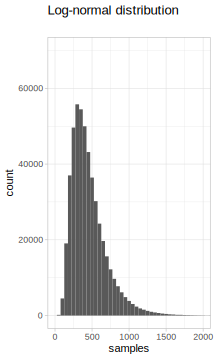
\includegraphics[width=0.48\linewidth]{bookdown_files/figure-latex/logndemo-1} 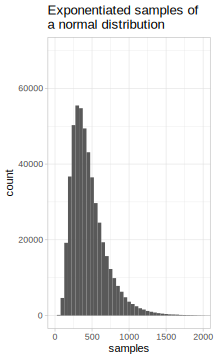
\includegraphics[width=0.48\linewidth]{bookdown_files/figure-latex/logndemo-2} \caption{Two log-normal distributions with the same parameters generated by either generating samples from a log-normal distribution or exponentiating samples from a normal distribution.}\label{fig:logndemo}
\end{figure}

\hypertarget{sec:lognormal}{%
\subsection{Re-fitting a single participant pressing a button repeatedly with a log-normal likelihood}\label{sec:lognormal}}

If we assume that reaction times are log-normally distributed, we'll need to change our likelihood function as follows:

\begin{equation}
rt_n \sim LogNormal(\mu,\sigma)
\end{equation}

But now the scale of our priors needs to change! We'll continue with the uniform priors for ease of exposition, even though, as we mentioned earlier, these are not recommended.

\begin{equation}
\begin{aligned}
\mu &\sim Uniform(0, 8) \\
\sigma &\sim Uniform(0, 1) \\
\end{aligned}
\label{eq:logpriorsunif}
\end{equation}

Because the parameters are in a different scale than the dependent variable, their interpretation changes and it is more complex than if we were dealing with a linear model that assumes a normal likelihood (location and scale do not coincide with the mean and standard deviation of the log-normal):

\begin{itemize}
\tightlist
\item
  \emph{The location, \(\mu\)}: In our previous linear model, \(\mu\) represented the grand mean (or the grand median, or grand mode, since in a normal distribution the three coincide). But now, the grand mean needs to be calculated in the following way, \(\exp(\mu +\sigma ^{2}/2)\). Interestingly, the grand median will just be \(\exp(\mu)\). We could assume that the grand median, \(\exp(\mu)\), represents the underlying time it takes to press the space bar if there would be no noise, that is, if \(\sigma\) would be 0. This also means that the prior of \(\mu\) is not in milliseconds, but in log(milliseconds).
\item
  \emph{The scale, \(\sigma\)}: This is the standard deviation of the normal distribution of \(\log(y)\). The standard deviation of a log-normal distribution with \emph{location} \(\mu\) and \emph{shape} \(\sigma\) will be \(\exp(\mu +\sigma ^{2}/2)\times \sqrt(\exp(\sigma^2)- 1)\). It's important to notice that, unlike the normal distribution, the spread of the log-normal distribution depends on both \(\mu\) and \(\sigma\).
\end{itemize}

To understand the meaning of our priors in milliseconds scale, we need to take into account both the priors and the likelihood. We can do this by generating a prior predictive distribution. Notice that we can just exponentiate the samples produced by \texttt{normal\_predictive\_distribution\_fast()} (or, alternatively, we could have edited the function and replaced \texttt{rnorm} for \texttt{rlnorm}).

\begin{Shaded}
\begin{Highlighting}[]
\NormalTok{N_samples <-}\StringTok{ }\DecValTok{1000}
\NormalTok{N_obs <-}\StringTok{ }\KeywordTok{nrow}\NormalTok{(df_noreading_data)}
\NormalTok{mu_samples <-}\StringTok{ }\KeywordTok{runif}\NormalTok{(N_samples, }\DecValTok{0}\NormalTok{, }\DecValTok{8}\NormalTok{)}
\NormalTok{sigma_samples <-}\StringTok{ }\KeywordTok{runif}\NormalTok{(N_samples, }\DecValTok{0}\NormalTok{, }\DecValTok{1}\NormalTok{)}
\NormalTok{prior_pred_ln <-}\StringTok{ }\KeywordTok{exp}\NormalTok{(}\KeywordTok{normal_predictive_distribution_fast}\NormalTok{(}
  \DataTypeTok{mu_samples =}\NormalTok{ mu_samples,}
  \DataTypeTok{sigma_samples =}\NormalTok{ sigma_samples,}
\NormalTok{  N_obs}
\NormalTok{))}
\end{Highlighting}
\end{Shaded}

And then we plot the distribution of some representative statistics:



\begin{Shaded}
\begin{Highlighting}[]
\NormalTok{prior_pred_ln }\OperatorTok
\StringTok{  }\KeywordTok{group_by}\NormalTok{(iter) }\OperatorTok
\StringTok{  }\KeywordTok{summarize}\NormalTok{(}
    \DataTypeTok{min_rt =} \KeywordTok{min}\NormalTok{(rt_pred),}
    \DataTypeTok{max_rt =} \KeywordTok{max}\NormalTok{(rt_pred),}
    \DataTypeTok{average_rt =} \KeywordTok{mean}\NormalTok{(rt_pred),}
    \DataTypeTok{median_rt =} \KeywordTok{median}\NormalTok{(rt_pred)}
\NormalTok{  ) }\OperatorTok
\StringTok{  }\KeywordTok{pivot_longer}\NormalTok{(}\DataTypeTok{cols =} \KeywordTok{ends_with}\NormalTok{(}\StringTok{"rt"}\NormalTok{), }\DataTypeTok{names_to =} \StringTok{"stat"}\NormalTok{, }\DataTypeTok{values_to =} \StringTok{"rt"}\NormalTok{) }\OperatorTok
\StringTok{  }\KeywordTok{ggplot}\NormalTok{(}\KeywordTok{aes}\NormalTok{(rt)) }\OperatorTok{+}
\StringTok{  }\KeywordTok{scale_x_continuous}\NormalTok{(}\StringTok{"Reaction times in ms"}\NormalTok{,}
    \DataTypeTok{trans =} \StringTok{"log"}\NormalTok{, }\DataTypeTok{breaks =} \KeywordTok{c}\NormalTok{(}\FloatTok{0.001}\NormalTok{, }\DecValTok{1}\NormalTok{, }\DecValTok{100}\NormalTok{, }\DecValTok{1000}\NormalTok{, }\DecValTok{10000}\NormalTok{, }\DecValTok{100000}\NormalTok{)}
\NormalTok{  ) }\OperatorTok{+}
\StringTok{  }\KeywordTok{geom_histogram}\NormalTok{() }\OperatorTok{+}
\StringTok{  }\KeywordTok{facet_wrap}\NormalTok{(}\OperatorTok{~}\NormalTok{stat, }\DataTypeTok{ncol =} \DecValTok{1}\NormalTok{)}
\end{Highlighting}
\end{Shaded}

\begin{figure}
\centering
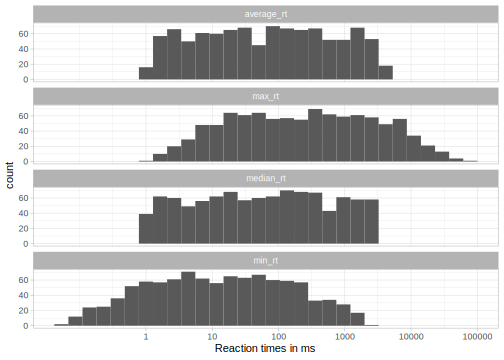
\includegraphics{bookdown_files/figure-latex/priorpredlogunif-1.pdf}
\caption{\label{fig:priorpredlogunif}Prior predictive distribution of averages, maximum, and minimum value of the log-normal model with priors defined in \eqref{eq:logpriorsunif}. Notice that the x-axis is log-transformed.}
\end{figure}

While we cannot not generate negative values anymore, since \(\exp(\)any number\() > 0\), and these priors might work, we can choose better regularizing priors for our model, such as the following:

\begin{equation}
\begin{aligned}
\mu &\sim Normal(6, 1.5) \\
\sigma &\sim Normal_+(0, 1) \\
\end{aligned}
\label{eq:logpriorsnorm}
\end{equation}

Notice that while \(\mu\) can be negative, the dependent variable won't, since the exponent of a negative value, \(\exp(\)some negative value\()\), is always greater than \(0\). Even before generating the prior predictive distributions, we can calculate the values within which we are 95\% sure that the expected median of the observations will lie. We do this by looking at what happens at two standard deviations away from the mean of the \emph{prior}, \(\mu\), that is \(6 - 2\times 1.5\) and \(6 + 2\times 1.5\), and exponentiating these values:

\begin{Shaded}
\begin{Highlighting}[]
\KeywordTok{c}\NormalTok{(}
  \DataTypeTok{lower =} \KeywordTok{exp}\NormalTok{(}\DecValTok{6} \OperatorTok{-}\StringTok{ }\DecValTok{2} \OperatorTok{*}\StringTok{ }\FloatTok{1.5}\NormalTok{),}
  \DataTypeTok{higher =} \KeywordTok{exp}\NormalTok{(}\DecValTok{6} \OperatorTok{+}\StringTok{ }\DecValTok{2} \OperatorTok{*}\StringTok{ }\FloatTok{1.5}\NormalTok{)}
\NormalTok{)}
\end{Highlighting}
\end{Shaded}

\begin{verbatim}
##  lower higher 
##     20   8103
\end{verbatim}

This means that our prior for \(\mu\) is still not too informative (these are medians; the actual values generated by the distribution can be much more spread out). We plot the distribution of some representative statistics in Figure \ref{fig:priorpredlognorm}.



\begin{Shaded}
\begin{Highlighting}[]
\NormalTok{N_samples <-}\StringTok{ }\DecValTok{1000}
\NormalTok{N_obs <-}\StringTok{ }\KeywordTok{nrow}\NormalTok{(df_noreading_data)}
\NormalTok{mu_samples <-}\StringTok{ }\KeywordTok{rnorm}\NormalTok{(N_samples, }\DecValTok{6}\NormalTok{, }\FloatTok{1.5}\NormalTok{)}
\NormalTok{sigma_samples <-}\StringTok{ }\KeywordTok{rtnorm}\NormalTok{(N_samples, }\DecValTok{0}\NormalTok{, }\DecValTok{1}\NormalTok{, }\DataTypeTok{a =} \DecValTok{0}\NormalTok{)}
\NormalTok{prior_pred_ln_better <-}\StringTok{ }\KeywordTok{exp}\NormalTok{(}\KeywordTok{normal_predictive_distribution_fast}\NormalTok{(}
  \DataTypeTok{mu_samples =}\NormalTok{ mu_samples,}
  \DataTypeTok{sigma_samples =}\NormalTok{ sigma_samples,}
\NormalTok{  N_obs}
\NormalTok{))}
\NormalTok{prior_pred_ln_better }\OperatorTok
\StringTok{  }\KeywordTok{group_by}\NormalTok{(iter) }\OperatorTok
\StringTok{  }\KeywordTok{summarize}\NormalTok{(}
    \DataTypeTok{min_rt =} \KeywordTok{min}\NormalTok{(rt_pred),}
    \DataTypeTok{max_rt =} \KeywordTok{max}\NormalTok{(rt_pred),}
    \DataTypeTok{average_rt =} \KeywordTok{mean}\NormalTok{(rt_pred),}
    \DataTypeTok{median_rt =} \KeywordTok{median}\NormalTok{(rt_pred)}
\NormalTok{  ) }\OperatorTok
\StringTok{ }\KeywordTok{pivot_longer}\NormalTok{(}\DataTypeTok{cols =} \KeywordTok{ends_with}\NormalTok{(}\StringTok{"rt"}\NormalTok{),}
              \DataTypeTok{names_to =} \StringTok{"stat"}\NormalTok{, }\DataTypeTok{values_to =} \StringTok{"rt"}\NormalTok{) }\OperatorTok
\StringTok{  }\KeywordTok{ggplot}\NormalTok{(}\KeywordTok{aes}\NormalTok{(rt)) }\OperatorTok{+}
\StringTok{  }\KeywordTok{scale_x_continuous}\NormalTok{(}\DataTypeTok{trans =} \StringTok{"log"}\NormalTok{, }\DataTypeTok{breaks =} \KeywordTok{c}\NormalTok{(}\FloatTok{0.001}\NormalTok{, }\DecValTok{1}\NormalTok{, }\DecValTok{100}\NormalTok{, }\DecValTok{1000}\NormalTok{, }\DecValTok{10000}\NormalTok{, }\DecValTok{100000}\NormalTok{)) }\OperatorTok{+}
\StringTok{  }\KeywordTok{geom_histogram}\NormalTok{() }\OperatorTok{+}
\StringTok{  }\KeywordTok{facet_wrap}\NormalTok{(}\OperatorTok{~}\NormalTok{stat, }\DataTypeTok{ncol =} \DecValTok{1}\NormalTok{) }\OperatorTok{+}
\StringTok{  }\KeywordTok{coord_cartesian}\NormalTok{(}\DataTypeTok{xlim =} \KeywordTok{c}\NormalTok{(}\FloatTok{0.001}\NormalTok{, }\DecValTok{300000}\NormalTok{))}
\end{Highlighting}
\end{Shaded}

\begin{figure}
\centering
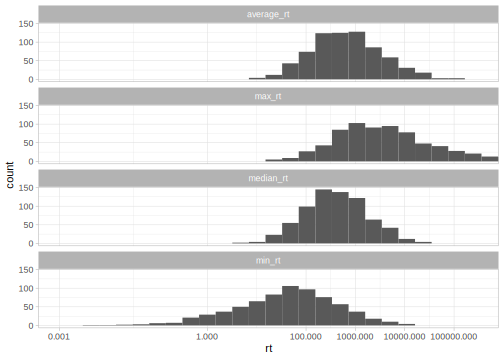
\includegraphics{bookdown_files/figure-latex/priorpredlognorm-1.pdf}
\caption{\label{fig:priorpredlognorm}Prior predictive distribution of averages, maximum, and minimum value of the log-normal model with priors defined in \eqref{eq:logpriorsnorm}. Notice that the x-axis is log-transformed.}
\end{figure}

We see that the priors that we are using are still too uninformative. We could do more iterations of choosing priors and generating posterior predictive distributions until we have priors that generate realistic data. However, for most cases, priors that generate data that whose statistics (mean, median, min, max, etc.) lie roughly in the correct order of magnitude are going to be acceptable.

We can fit the model now, but notice that we need to specify that the family is \texttt{lognormal()}. In our first example, we had used the family \texttt{gaussian()}.

\begin{Shaded}
\begin{Highlighting}[]
\NormalTok{fit_press_ln <-}\StringTok{ }\KeywordTok{brm}\NormalTok{(rt }\OperatorTok{~}\StringTok{ }\DecValTok{1}\NormalTok{,}
  \DataTypeTok{data =}\NormalTok{ df_noreading_data,}
  \DataTypeTok{family =} \KeywordTok{lognormal}\NormalTok{(),}
  \DataTypeTok{prior =} \KeywordTok{c}\NormalTok{(}
    \KeywordTok{prior}\NormalTok{(}\KeywordTok{normal}\NormalTok{(}\DecValTok{6}\NormalTok{, }\FloatTok{1.5}\NormalTok{), }\DataTypeTok{class =}\NormalTok{ Intercept),}
    \KeywordTok{prior}\NormalTok{(}\KeywordTok{normal}\NormalTok{(}\DecValTok{0}\NormalTok{, }\DecValTok{1}\NormalTok{), }\DataTypeTok{class =}\NormalTok{ sigma)}
\NormalTok{  )}
\NormalTok{)}
\end{Highlighting}
\end{Shaded}

When we look at the summary of the posterior, the parameters are in log-scale:

\begin{Shaded}
\begin{Highlighting}[]
\NormalTok{fit_press_ln}
\end{Highlighting}
\end{Shaded}

\begin{verbatim}
##  Family: lognormal 
##   Links: mu = identity; sigma = identity 
## Formula: rt ~ 1 
##    Data: df_noreading_data (Number of observations: 361) 
## Samples: 4 chains, each with iter = 2000; warmup = 1000; thin = 1;
##          total post-warmup samples = 4000
## 
## Population-Level Effects: 
##           Estimate Est.Error l-95% CI u-95% CI Rhat
## Intercept     5.12      0.01     5.10     5.13 1.00
##           Bulk_ESS Tail_ESS
## Intercept     4198     2798
## 
## Family Specific Parameters: 
##       Estimate Est.Error l-95% CI u-95% CI Rhat
## sigma     0.13      0.00     0.13     0.14 1.00
##       Bulk_ESS Tail_ESS
## sigma     2906     2732
## 
## Samples were drawn using sampling(NUTS). For each parameter, Eff.Sample 
## is a crude measure of effective sample size, and Rhat is the potential 
## scale reduction factor on split chains (at convergence, Rhat = 1).
\end{verbatim}

If we want to know how long does it take to press the space bar in milliseconds, we need to transform the \(\mu\) (or \texttt{Intercept} in the model) to milliseconds. Since we know that the median of the log-normal distribution is \(exp(\mu)\), we do the following to calculate an estimate in milliseconds:

\begin{Shaded}
\begin{Highlighting}[]
\NormalTok{estimate_ms <-}\StringTok{ }\KeywordTok{exp}\NormalTok{(}\KeywordTok{posterior_samples}\NormalTok{(fit_press_ln)}\OperatorTok{$}\NormalTok{b_Intercept)}
\end{Highlighting}
\end{Shaded}

If we want to know the mean and 95\% credible interval, we do the following:

\begin{Shaded}
\begin{Highlighting}[]
\KeywordTok{c}\NormalTok{(}\DataTypeTok{mean =} \KeywordTok{mean}\NormalTok{(estimate_ms), }\KeywordTok{quantile}\NormalTok{(estimate_ms, }\DataTypeTok{probs =} \KeywordTok{c}\NormalTok{(.}\DecValTok{025}\NormalTok{, }\FloatTok{.975}\NormalTok{)))}
\end{Highlighting}
\end{Shaded}

\begin{verbatim}
## mean 2.5%  98% 
##  167  165  169
\end{verbatim}

We can now verify whether our predicted datasets look similar to
the real dataset. See Figure \ref{fig:lognppc}; compare this with the earlier Figure \ref{fig:normalppc2}.



\begin{Shaded}
\begin{Highlighting}[]
\KeywordTok{pp_check}\NormalTok{(fit_press_ln, }\DataTypeTok{nsamples =} \DecValTok{100}\NormalTok{)}
\end{Highlighting}
\end{Shaded}

\begin{figure}
\centering
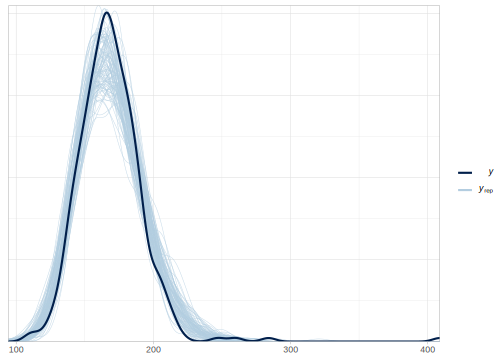
\includegraphics{bookdown_files/figure-latex/lognppc-1.pdf}
\caption{\label{fig:lognppc}Posterior predictive distribution of \texttt{m\_noreading\_ln}}
\end{figure}

\emph{Are the posterior predicted data now more similar to the real data, compared to the case where we had a Normal likelihood?}

It seems so, but it's not easy to tell. Another way to examine this would be to look at the distribution of summary statistics. We compare the distribution of representative summary statistics for the datasets generated by different models and compare them to the observed statistics. We suspect that the normal distribution would generate reaction times that are too fast (since it's symmetrical) and that the log-normal distribution may capture the long tail better than the normal model. Based on our hunch, we compute the distribution of minimum and maximum values for the posterior predictive distributions, and we compare them with the minimum and maximum value respectively in the data.

\begin{Shaded}
\begin{Highlighting}[]
\KeywordTok{pp_check}\NormalTok{(fit_press, }\DataTypeTok{type =} \StringTok{"stat"}\NormalTok{, }\DataTypeTok{stat =} \StringTok{"min"}\NormalTok{) }\OperatorTok{+}\StringTok{ }\KeywordTok{ggtitle}\NormalTok{(}\StringTok{"Normal model"}\NormalTok{)}
\KeywordTok{pp_check}\NormalTok{(fit_press_ln, }\DataTypeTok{type =} \StringTok{"stat"}\NormalTok{, }\DataTypeTok{stat =} \StringTok{"min"}\NormalTok{) }\OperatorTok{+}\StringTok{ }\KeywordTok{ggtitle}\NormalTok{(}\StringTok{"Log-normal model"}\NormalTok{)}
\end{Highlighting}
\end{Shaded}

\begin{figure}
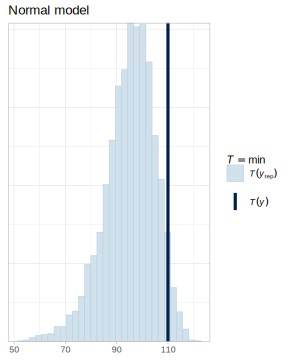
\includegraphics[width=0.45\linewidth]{bookdown_files/figure-latex/ppcheckmin-1} 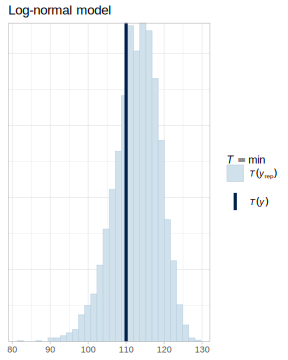
\includegraphics[width=0.45\linewidth]{bookdown_files/figure-latex/ppcheckmin-2} \caption{Distribution of minimum values in a posterior predictive check. The minimum in the data is 110 ms.}\label{fig:ppcheckmin}
\end{figure}

\begin{Shaded}
\begin{Highlighting}[]
\KeywordTok{pp_check}\NormalTok{(fit_press, }\DataTypeTok{type =} \StringTok{"stat"}\NormalTok{, }\DataTypeTok{stat =} \StringTok{"max"}\NormalTok{) }\OperatorTok{+}\StringTok{ }\KeywordTok{ggtitle}\NormalTok{(}\StringTok{"Normal model"}\NormalTok{)}
\KeywordTok{pp_check}\NormalTok{(fit_press_ln, }\DataTypeTok{type =} \StringTok{"stat"}\NormalTok{, }\DataTypeTok{stat =} \StringTok{"max"}\NormalTok{) }\OperatorTok{+}\StringTok{ }\KeywordTok{ggtitle}\NormalTok{(}\StringTok{"Log-normal model"}\NormalTok{)}
\end{Highlighting}
\end{Shaded}

\begin{figure}
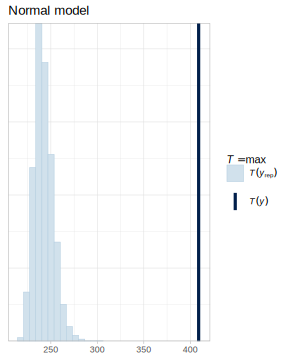
\includegraphics[width=0.45\linewidth]{bookdown_files/figure-latex/ppcheckmax-1} 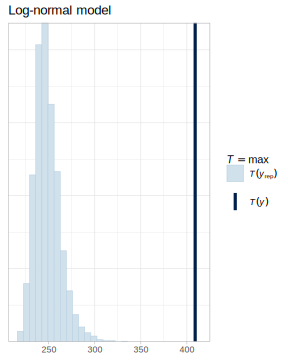
\includegraphics[width=0.45\linewidth]{bookdown_files/figure-latex/ppcheckmax-2} \caption{Distribution of maximum values in a posterior predictive check. The maximum in the data is 409 ms.}\label{fig:ppcheckmax}
\end{figure}

Figure \ref{fig:ppcheckmin} shows that the log-normal likelihood does a slightly better job since the minimum value is contained in the bulk of the log-normal distribution and in the tail of normal one. Figure \ref{fig:ppcheckmax} shows that both models are unable to capture the maximum value of the observed data. One explanation for this is that the log-normal-ish observations in our data are being generated by the task of pressing as fast as possible, while the observations with long reaction times are being generated by lapses of attention.

\hypertarget{summary}{%
\section{Summary}\label{summary}}

\hypertarget{further-reading-2}{%
\section{Further reading}\label{further-reading-2}}

On the topic of priors:

\begin{itemize}
\tightlist
\item
  Chapter 5 of Lunn D, Jackson C, Spiegelhalter DJ, Best N,, Thomas A (2012). \emph{The BUGS book: A practical, introduction to Bayesian analysis}, volume 98., CRC Press.
\item
  Gelman A, Simpson D, Betancourt M (2017). ``The, prior can often only be understood in the, context of the likelihood.'' \emph{Entropy}, \emph{19}(10),, 555. doi: 10.3390/e19100555 (URL:, \url{https://doi.org/10.3390/e19100555}), \textless{}URL:, \url{https://www.mdpi.com/1099-4300/19/10/555}\textgreater{}.
\item
  Simpson D, Rue H, Riebler A, Martins TG, Sørbye, SH (2017). ``Penalising Model Component, Complexity: A Principled, Practical Approach to, Constructing Priors.'' \emph{Statistical Science},, \emph{32}(1), 1-28. ISSN 0883-4237, 2168-8745, doi:, 10.1214/16-STS576 (URL:, \url{https://doi.org/10.1214/16-STS576}), \textless{}URL:, \url{https://projecteuclid.org/euclid.ss/1491465621}\textgreater{}.
\item
  Prior Distributions for rstanarm Models in \url{https://mc-stan.org/rstanarm/articles/priors.html}
\item
  Prior Choice Recommendations in \url{https://github.com/stan-dev/stan/wiki/Prior-Choice-Recommendations}
\end{itemize}

\hypertarget{exercises-2}{%
\section{Exercises}\label{exercises-2}}

\begin{enumerate}
\def\labelenumi{\arabic{enumi}.}
\tightlist
\item
  Can you find priors on \(\mu\) that have an undesirable impact in our estimates for the model with normal likelihood? And for the model with the log-normal likelihood?
\item
  For the log-normal model, change the prior of \(\sigma\) to .5 and generate prior predictive distributions.
\item
  For the log-normal model, try to find sensible priors with prior predictive checks.
\item
  For the log-normal model, what is the mean (rather than median) time that takes to press the space bar, what is the standard deviation of the reaction times in milliseconds?
\end{enumerate}

\hypertarget{appendix}{%
\section{Appendix}\label{appendix}}

\hypertarget{generating-prior-predictive-distributions-with-brms}{%
\subsection{\texorpdfstring{Generating prior predictive distributions with \texttt{brms}}{Generating prior predictive distributions with brms}}\label{generating-prior-predictive-distributions-with-brms}}

\texttt{brms} can generate prior predictive distributions for us ignoring the data, by using \texttt{sample\_prior\ =\ "only"}. Since we are not fitting any model, we can ignore the messages and warnings, and we set only one chain with 1000 iterations and no warmup. \texttt{posterior\_predict(...)} and \texttt{predict(...,\ summary\ =\ FALSE)} will return an array of N samples by N observations of prior predictions (this is because of \texttt{sample\_prior\ =\ "only"}), and we'll need to manipulate the array to get the desired data frame.

\begin{Shaded}
\begin{Highlighting}[]
\NormalTok{fit_press_prior <-}\StringTok{ }\KeywordTok{brm}\NormalTok{(rt }\OperatorTok{~}\StringTok{ }\DecValTok{1}\NormalTok{,}
  \DataTypeTok{family =} \KeywordTok{gaussian}\NormalTok{(),}
  \DataTypeTok{prior =} \KeywordTok{c}\NormalTok{(}
    \KeywordTok{prior}\NormalTok{(}\KeywordTok{uniform}\NormalTok{(}\DecValTok{0}\NormalTok{, }\DecValTok{60000}\NormalTok{), }\DataTypeTok{class =}\NormalTok{ Intercept),}
    \KeywordTok{prior}\NormalTok{(}\KeywordTok{uniform}\NormalTok{(}\DecValTok{0}\NormalTok{, }\DecValTok{2000}\NormalTok{), }\DataTypeTok{class =}\NormalTok{ sigma)}
\NormalTok{  ),}
  \DataTypeTok{sample_prior =} \StringTok{"only"}\NormalTok{,}
  \DataTypeTok{warmup =} \DecValTok{0}\NormalTok{,}
  \DataTypeTok{chains =} \DecValTok{1}\NormalTok{,}
  \DataTypeTok{iter =} \DecValTok{1000}\NormalTok{,}
  \DataTypeTok{data =}\NormalTok{ df_noreading_data}
\NormalTok{)}

\CommentTok{# predict with summary = FALSE returns a N_samples * N_obs array:}
\NormalTok{prior_pred <-}\StringTok{ }\KeywordTok{predict}\NormalTok{(fit_press_prior, }\DataTypeTok{summary =} \OtherTok{FALSE}\NormalTok{) }\OperatorTok
\StringTok{  }\CommentTok{# array_banch converts it in a list of N_samples elements,}
\StringTok{  }\CommentTok{# and in each element a dataset of N_obs:}
\StringTok{  }\KeywordTok{array_branch}\NormalTok{(}\DecValTok{1}\NormalTok{) }\OperatorTok
\StringTok{  }\CommentTok{# map_dfr loops over the N_sample elements of the list and builds a data frame}
\StringTok{  }\KeywordTok{map_dfr}\NormalTok{(}\OperatorTok{~}\StringTok{ }\KeywordTok{tibble}\NormalTok{(}\DataTypeTok{rt_pred =}\NormalTok{ .x, }\DataTypeTok{trialn =} \KeywordTok{seq_along}\NormalTok{(.x)), }\DataTypeTok{.id =} \StringTok{"sample_n"}\NormalTok{) }\OperatorTok
\StringTok{  }\CommentTok{# .id is always a string and needs to be converted}
\StringTok{  }\KeywordTok{mutate}\NormalTok{(}\DataTypeTok{sample_n =} \KeywordTok{as.numeric}\NormalTok{(sample_n))}
\end{Highlighting}
\end{Shaded}

\hypertarget{bayesian-regression-models}{%
\chapter{Bayesian regression models}\label{bayesian-regression-models}}

We generally run experiments because we are interested in the relationship between two or more observables. A regression will tell us how our \emph{dependent variable}, also called the \emph{response} or \emph{outcome variable} (e.g., pupil size, reaction times, accuracy, etc) is affected by one or many \emph{independent variables}, \emph{predictors}, or \emph{explanatory variables}. Predictors can be categorical (e.g., male or female), ordinal (first, second, third, etc), or continuous. We will assume that our predictors are continuous in this chapter, and we will refer to them (mostly) as \emph{covariates}. Unfortunately, many times it will happen that the same concept has different names, and a name can be associated with different concepts (mostly depending on the context). \emph{Covariates} are sometimes used to refer to control variables; we won't use them with this meaning in the book, but it's a good idea to bear this in mind.

\BeginKnitrBlock{rmdnote}
to-do: This could be expanded much more.
\EndKnitrBlock{rmdnote}

\hypertarget{sec:pupil}{%
\section{A first linear model: Does attentional load affect pupil size?}\label{sec:pupil}}

We'll look at the effect of cognitive processing on human pupil size to illustrate the use of Bayesian linear regression models. Although pupil size is mostly related to the amount of light that reaches the retina or the distance to a perceived object, pupil sizes are also systematically influenced by cognitive processing: It has been found that increased cognitive load leads to an increase in the pupil size \citep[for a review, see][]{mathotPupillometryPsychologyPhysiology2018}.

For this example, we'll use the data of one participant's pupil size of the control experiment of \citet{wahnPupilSizesScale2016} averaged by trial.\footnote{The full dataset can be found in \url{https://osf.io/z43dz/}. We show our preprocessing in the appendix of this chapter, section \ref{sec:preprocessingpupil}.}
In this experiment, a participant covertly tracked between zero and five objects among several randomly moving objects on a computer screen. In this task, called multiple object tracking {[}or \href{mailto:MOT;@pylyshynTrackingMultipleIndependent1988}{\nolinkurl{MOT;@pylyshynTrackingMultipleIndependent1988}}{]} task, several objects appear in the screen, and a subset of them
are indicated as ``targets'' at the beginning. Then, the objects start moving randomly across the screen and become indistinguishable. After several seconds, the objects stop moving and the participant needs to indicate which objects were the targets. See also Figure \ref{fig:mot}. Our research goal is to examine how the number of moving objects being tracked, that is how the attentional load, affects pupil size.



\begin{figure}

{\centering 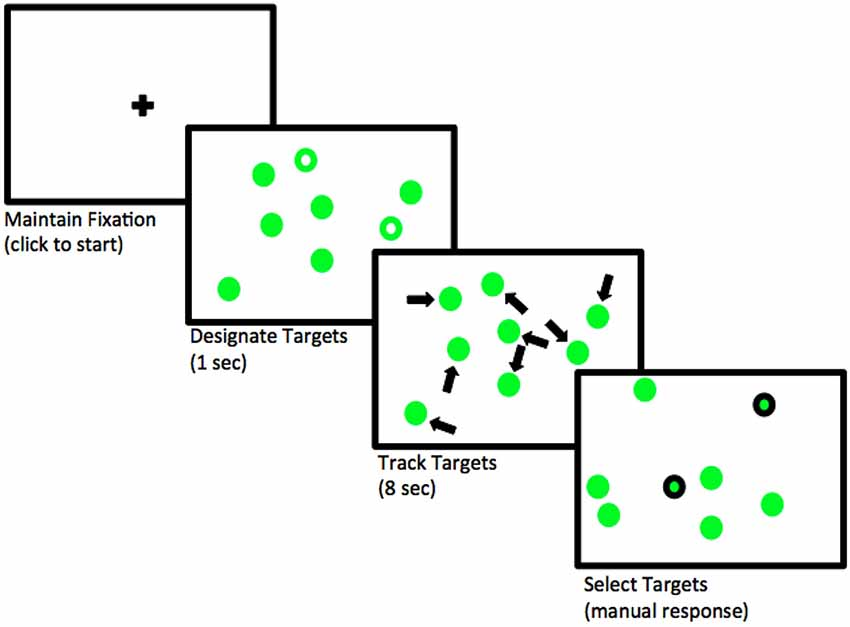
\includegraphics[width=0.8\linewidth]{cc_figure/MOT} 

}

\caption{Flow of events in a trial where two objects needs to be tracked. Adapted from \citet{Blumberg2015}; licensed under CC BY 4.0.}\label{fig:mot}
\end{figure}

\hypertarget{likelihood-and-priors}{%
\subsection{Likelihood and priors}\label{likelihood-and-priors}}

We will model pupil size as normally distributed, because we are not expecting a skew, and we have no further information available about the distribution of pupil sizes. (Notice that pupil sizes cannot be of size zero or negative, so we know for sure that this choice is not exactly right.) For simplicity, we are also going to assume a linear relationship between load and the pupil size.

Let's summarize our assumptions:

\begin{enumerate}
\def\labelenumi{\arabic{enumi}.}
\tightlist
\item
  There is some average pupil size represented by \(\alpha\).
\item
  The increase of attentional load has a linear relationship with pupil size, determined by \(\beta\).
\item
  There is some noise in this process, that is, variability around the true pupil size i.e., a scale, \(\sigma\).
\item
  The noise is normally distributed.
\end{enumerate}

Our likelihood will be as follows:

\begin{equation}
p\_size_n \sim Normal(\alpha + c\_load_n \cdot \beta,\sigma)
\end{equation}

where \(n\) indicates the observation number with \(n = 1 \ldots N\)

This means that the formula that we'll use in \texttt{brms} will be \texttt{p\_size\ \textasciitilde{}\ 1\ +\ c\_load}, where \texttt{1} represents the intercept, \(\alpha\), which doesn't depend on a covariate or predictor, and \texttt{c\_load} is our covariate that is multiplied by \(\beta\). We will generally indicate with the prefix \texttt{c\_}, that a covariate (in this case load) is centered (i.e., we subtract from each value the mean of all values). If load is centered, the intercept represents the pupil size at the average load in the experiment (because at the average load, the centered load is zero, and then \(\alpha + 0 \cdot \beta\)). Alternatively, if the load would not have been centered (i.e., starts with no load, then one, two, etc), then the intercept would represent the pupil size when there is no load. Although this formula would be enough to fit a frequentist model with \texttt{lm(p\_size\ \textasciitilde{}\ 1\ +\ c\_load,\ dataset)}, when we fit a Bayesian model, we have to specify priors for each of the parameters.

For setting the priors, we need information about pupil sizes. While we might know that pupil sizes range between 2 and 5 millimeters \citep{reference}, this experiment was conducted with the Eyelink-II eyetracker which measures the pupils in arbitrary units \citep{hayesMappingCorrectingInfluence2016}. If this is our first analysis of pupil size, before setting up the priors, we'll need to look at some measures of pupil size. (If we had analyzed this type of data before, we could also look at estimates from previous experiments). Fortunately, we have some measurements of the same participant with no attentional load for the first 100ms, each 10 ms, in \texttt{pupil\_pilot.csv}: This will give us some idea about the order of magnitude of our dependent variable.

\begin{Shaded}
\begin{Highlighting}[]
\NormalTok{df_pupil_pilot <-}\StringTok{ }\KeywordTok{read_csv}\NormalTok{(}\StringTok{"./data/pupil_pilot.csv"}\NormalTok{)}
\NormalTok{df_pupil_pilot}\OperatorTok{$}\NormalTok{p_size }\OperatorTok\StringTok{ }\KeywordTok{summary}\NormalTok{()}
\end{Highlighting}
\end{Shaded}

\begin{verbatim}
##    Min. 1st Qu.  Median    Mean 3rd Qu.    Max. 
##     852     856     862     861     866     868
\end{verbatim}

With this information we can set a regularizing prior for \(\alpha\). We center the prior around 1000 to be in the right order of magnitude.\footnote{The average pupil size will probably be higher than 800, since this measurement was with no load, but, in any case, the exact number won't matter, any mean between 500-1500 would be fine if the standard deviation is large.} Since we don't know how much pupil sizes are going to vary by load yet, we include a rather wide prior by defining it as a normally distribution and setting its standard deviation as \(500\).

\begin{equation}
\alpha \sim Normal(1000, 500) 
\end{equation}

Given that our covariate load is centered, with the prior for \(\alpha\), we are saying that we suspect that the average pupil size for the average load in the experiment will be in a 95\% central interval limited by approximately \(1000 \pm 2 \cdot 500 = [20, 2000]\) units. We can caclulate this in \texttt{R} using the \texttt{qnorm} function:

\begin{Shaded}
\begin{Highlighting}[]
\KeywordTok{c}\NormalTok{(}\KeywordTok{qnorm}\NormalTok{(.}\DecValTok{025}\NormalTok{, }\DecValTok{1000}\NormalTok{,}\DecValTok{500}\NormalTok{), }\KeywordTok{qnorm}\NormalTok{(.}\DecValTok{975}\NormalTok{, }\DecValTok{1000}\NormalTok{, }\DecValTok{500}\NormalTok{))}
\end{Highlighting}
\end{Shaded}

\begin{verbatim}
## [1]   20 1980
\end{verbatim}

We know that the measurements of the pilot data are strongly correlated because they were taken together just some milliseconds apart. For this reason, they won't tell us how much the pupil size can vary. We set up a quite weak prior for \(\sigma\) that encodes our lack of precise information: \(\sigma\) is surely larger than zero and has to be in the order of magnitude of the pupil size with no load.

\begin{equation}
\sigma \sim Normal_+(0, 1000)
\end{equation}

With this prior for \(\sigma\), we are saying that we expect that the standard deviation of the pupil sizes should be in the following 95\% central interval. (Notice that we use \texttt{qtnorm(...,\ a\ =\ 0)} and not \texttt{qnorm()}).

\begin{Shaded}
\begin{Highlighting}[]
\KeywordTok{c}\NormalTok{(}\KeywordTok{qtnorm}\NormalTok{(.}\DecValTok{025}\NormalTok{, }\DecValTok{0}\NormalTok{, }\DecValTok{1000}\NormalTok{, }\DataTypeTok{a =} \DecValTok{0}\NormalTok{), }\KeywordTok{qtnorm}\NormalTok{(.}\DecValTok{975}\NormalTok{, }\DecValTok{70}\NormalTok{,}\DecValTok{1000}\NormalTok{, }\DataTypeTok{a =} \DecValTok{0}\NormalTok{))}
\end{Highlighting}
\end{Shaded}

\begin{verbatim}
## [1]   31 2290
\end{verbatim}

We still need to set a prior for \(\beta\), the change in pupil size produced by the attentional load. Given that pupil size changes are not easily perceptible (we don't see them in our day-to-day life), we expect them to be much smaller than the pupil size, so we use the following prior:

\begin{equation}
\beta \sim Normal(0, 100)
\end{equation}

With the prior of \(\beta\), we are saying that we don't really know if the attentional load will increase or even decrease the pupil size (notice that is centered in zero), but we do know that one unit of load (that is one more object to track) will potentially change the pupil size in a way that is consistent with the following 95\% central interval.

\begin{Shaded}
\begin{Highlighting}[]
\KeywordTok{c}\NormalTok{(}\KeywordTok{qnorm}\NormalTok{(.}\DecValTok{025}\NormalTok{, }\DecValTok{0}\NormalTok{,}\DecValTok{100}\NormalTok{), }\KeywordTok{qnorm}\NormalTok{(.}\DecValTok{975}\NormalTok{, }\DecValTok{0}\NormalTok{,}\DecValTok{100}\NormalTok{))}
\end{Highlighting}
\end{Shaded}

\begin{verbatim}
## [1] -196  196
\end{verbatim}

That is, we don't expect changes in size that increase or decrease the pupil size in more than 200 units.

\BeginKnitrBlock{rmdnote}
to-do: maybe prior predictive distributions here??
\EndKnitrBlock{rmdnote}

\hypertarget{the-brms-model}{%
\subsection{\texorpdfstring{The \texttt{brms} model}{The brms model}}\label{the-brms-model}}

Before fitting the \texttt{brms} model, we load the data and center the predictor \texttt{load}:

\begin{Shaded}
\begin{Highlighting}[]
\NormalTok{df_pupil_data <-}\StringTok{ }\KeywordTok{read_csv}\NormalTok{(}\StringTok{"data/pupil.csv"}\NormalTok{)}
\NormalTok{df_pupil_data <-}\StringTok{ }\NormalTok{df_pupil_data }\OperatorTok
\StringTok{    }\KeywordTok{mutate}\NormalTok{(}\DataTypeTok{c_load =}\NormalTok{ load }\OperatorTok{-}\StringTok{ }\KeywordTok{mean}\NormalTok{(load))}
\NormalTok{df_pupil_data}
\end{Highlighting}
\end{Shaded}

\begin{verbatim}
## # A tibble: 41 x 4
##   trial  load p_size c_load
##   <dbl> <dbl>  <dbl>  <dbl>
## 1     1     2  1021. -0.439
## 2     2     1   951. -1.44 
## 3     3     5  1064.  2.56 
## 4     4     4   913.  1.56 
## 5     5     0   603. -2.44 
## # ... with 36 more rows
\end{verbatim}

Now we can fit the \texttt{brms} model:

\begin{Shaded}
\begin{Highlighting}[]
\NormalTok{fit_pupil <-}\StringTok{ }\KeywordTok{brm}\NormalTok{(p_size }\OperatorTok{~}\StringTok{ }\DecValTok{1} \OperatorTok{+}\StringTok{ }\NormalTok{c_load,}
                 \DataTypeTok{data =}\NormalTok{ df_pupil_data,}
                 \DataTypeTok{family =} \KeywordTok{gaussian}\NormalTok{(),}
                 \DataTypeTok{prior =} \KeywordTok{c}\NormalTok{(}
                     \KeywordTok{prior}\NormalTok{(}\KeywordTok{normal}\NormalTok{(}\DecValTok{1000}\NormalTok{, }\DecValTok{500}\NormalTok{), }\DataTypeTok{class =}\NormalTok{ Intercept),}
                     \KeywordTok{prior}\NormalTok{(}\KeywordTok{normal}\NormalTok{(}\DecValTok{0}\NormalTok{, }\DecValTok{1000}\NormalTok{), }\DataTypeTok{class =}\NormalTok{ sigma),}
                     \KeywordTok{prior}\NormalTok{(}\KeywordTok{normal}\NormalTok{(}\DecValTok{0}\NormalTok{, }\DecValTok{100}\NormalTok{), }\DataTypeTok{class =}\NormalTok{ b, }\DataTypeTok{coef =}\NormalTok{ c_load)}
\NormalTok{                 )) }
\end{Highlighting}
\end{Shaded}

The only difference from our previous models is that we now have a predictor in the formula and in the priors. Priors for predictors are indicated with \texttt{class\ =\ b}, and the specific predictor with \texttt{coef\ =\ c\_load}. If we want to set the same priors to different predictors we can omit the argument \texttt{coef}. We can remove the \texttt{1} of the formula, and \texttt{brm()} will fit the exact same model as when we specify \texttt{1} explicitly. If we really want to remove the intercept we indicate this with \texttt{0\ +...} or \texttt{-1\ +...}. See also the box \ref{thm:intercept} for more details about the treatment of the intercepts by \texttt{brms}.

We can inspect the output of our model now:

\begin{Shaded}
\begin{Highlighting}[]
\KeywordTok{plot}\NormalTok{(fit_pupil)}
\end{Highlighting}
\end{Shaded}

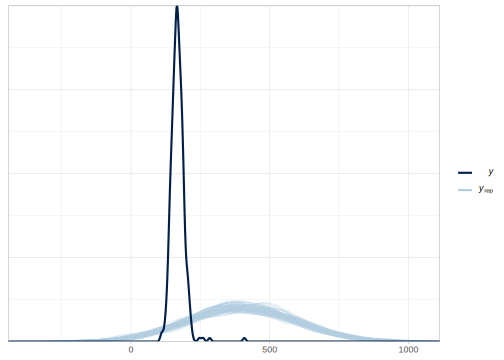
\includegraphics{bookdown_files/figure-latex/unnamed-chunk-83-1.pdf}

\begin{Shaded}
\begin{Highlighting}[]
\NormalTok{fit_pupil}
\end{Highlighting}
\end{Shaded}

\begin{verbatim}
##  Family: gaussian 
##   Links: mu = identity; sigma = identity 
## Formula: p_size ~ 1 + c_load 
##    Data: df_pupil_data (Number of observations: 41) 
## Samples: 4 chains, each with iter = 2000; warmup = 1000; thin = 1;
##          total post-warmup samples = 4000
## 
## Population-Level Effects: 
##           Estimate Est.Error l-95% CI u-95% CI Rhat
## Intercept   701.68     20.56   660.21   741.57 1.00
## c_load       33.82     11.70    10.26    56.83 1.00
##           Bulk_ESS Tail_ESS
## Intercept     3444     2684
## c_load        3769     2912
## 
## Family Specific Parameters: 
##       Estimate Est.Error l-95% CI u-95% CI Rhat
## sigma   128.49     14.82   103.07   161.81 1.00
##       Bulk_ESS Tail_ESS
## sigma     2946     2822
## 
## Samples were drawn using sampling(NUTS). For each parameter, Eff.Sample 
## is a crude measure of effective sample size, and Rhat is the potential 
## scale reduction factor on split chains (at convergence, Rhat = 1).
\end{verbatim}

We discuss how we could communicate the relevant information in the next section.

\Begin{extra}

\BeginKnitrBlock{theorem}
\protect\hypertarget{thm:intercept}{}{\label{thm:intercept} }\textbf{Intercepts in \texttt{brms}}
\EndKnitrBlock{theorem}

When we set up a prior for the intercept in \texttt{brms}, we actually set a prior for an intercept given that all the predictors are centered. This did not matter in our previous examples because we centered our predictor (or we had none), but it might matter if we want to have uncentered predictors. In the design we are discussing, a non-centered predictor of load will mean that the intercept, \(\alpha\), has a straightforward interpretation (in many cases, however, an intercept with a non-centered predictor won't have a straightforward interpretation): the pupil size when there is no attention load.

We might be more sure about prior values for the no load condition, and we want to set the following prior to our new \(\alpha\): \(Normal(800,200)\). In this case, we should fit the following model:

\begin{Shaded}
\begin{Highlighting}[]
\NormalTok{fit_pupil_non_centered <-}\StringTok{ }\KeywordTok{brm}\NormalTok{(p_size }\OperatorTok{~}\StringTok{ }\DecValTok{0} \OperatorTok{+}\StringTok{ }\NormalTok{intercept }\OperatorTok{+}\StringTok{ }\NormalTok{load,}
                 \DataTypeTok{data =}\NormalTok{ df_pupil_data,}
                 \DataTypeTok{family =} \KeywordTok{gaussian}\NormalTok{(),}
                 \DataTypeTok{prior =} \KeywordTok{c}\NormalTok{(}
                     \KeywordTok{prior}\NormalTok{(}\KeywordTok{normal}\NormalTok{(}\DecValTok{800}\NormalTok{, }\DecValTok{200}\NormalTok{), }\DataTypeTok{class =}\NormalTok{ b, }\DataTypeTok{coef =}\NormalTok{ intercept),}
                     \KeywordTok{prior}\NormalTok{(}\KeywordTok{normal}\NormalTok{(}\DecValTok{0}\NormalTok{, }\DecValTok{1000}\NormalTok{), }\DataTypeTok{class =}\NormalTok{ sigma),}
                     \KeywordTok{prior}\NormalTok{(}\KeywordTok{normal}\NormalTok{(}\DecValTok{0}\NormalTok{, }\DecValTok{100}\NormalTok{), }\DataTypeTok{class =}\NormalTok{ b, }\DataTypeTok{coef =}\NormalTok{ load)}
\NormalTok{                 ))}
\end{Highlighting}
\end{Shaded}

Notice that we remove the regular centered intercept by adding \texttt{0} to the formula, and we replace it with the ``actual'' intercept we want to set priors to with \texttt{intercept}---this is a reserved word, and thus we cannot name any predictor with this name. This new parameter is also of the class \texttt{b}, so its prior needs to be defined accordingly.

The output below shows that, as expected, while the posterior for the intercept has changed noticeably, the posterior for the effect of load remains virtually unchanged.

\begin{Shaded}
\begin{Highlighting}[]
\KeywordTok{posterior_summary}\NormalTok{(fit_pupil_non_centered)}
\end{Highlighting}
\end{Shaded}

\begin{verbatim}
##             Estimate Est.Error   Q2.5 Q97.5
## b_intercept      623      34.3  557.3   691
## b_load            33      11.7    9.8    56
## sigma            129      15.2  104.0   163
## lp__            -271       1.2 -274.1  -270
\end{verbatim}

Notice the following potential pitfall. A model like the one below will fit a non-centered load predictor, but will assign a prior of \(Normal(800,200)\) to the intercept of a \emph{centered} model, \(\alpha_{centered}\), and not the current intercept, \(\alpha\).

\begin{Shaded}
\begin{Highlighting}[]
\NormalTok{fit_pupil_wrong <-}\StringTok{ }\KeywordTok{brm}\NormalTok{(p_size }\OperatorTok{~}\StringTok{ }\DecValTok{1} \OperatorTok{+}\StringTok{ }\NormalTok{load,}
                 \DataTypeTok{data =}\NormalTok{ df_pupil_data,}
                 \DataTypeTok{family =} \KeywordTok{gaussian}\NormalTok{(),}
                 \DataTypeTok{prior =} \KeywordTok{c}\NormalTok{(}
                     \KeywordTok{prior}\NormalTok{(}\KeywordTok{normal}\NormalTok{(}\DecValTok{800}\NormalTok{, }\DecValTok{100}\NormalTok{), }\DataTypeTok{class =}\NormalTok{ Intercept),}
                     \KeywordTok{prior}\NormalTok{(}\KeywordTok{normal}\NormalTok{(}\DecValTok{0}\NormalTok{, }\DecValTok{1000}\NormalTok{), }\DataTypeTok{class =}\NormalTok{ sigma),}
                     \KeywordTok{prior}\NormalTok{(}\KeywordTok{normal}\NormalTok{(}\DecValTok{0}\NormalTok{, }\DecValTok{100}\NormalTok{), }\DataTypeTok{class =}\NormalTok{ b, }\DataTypeTok{coef =}\NormalTok{ load)}
\NormalTok{                 ))}
\end{Highlighting}
\end{Shaded}

What does it mean to set a prior to \(\alpha_{centered}\) in a model that \emph{doesn't} include \(\alpha_{centered}\)?

Notice that the fitted values of the non-centered model and the centered one are identical, that is, the expected values of the response distribution without the residual error (when \(\sigma =0\)) are identical for both models:

\begin{equation}
\alpha + load_n \cdot \beta = \alpha_{centered} + (load_n - mean(load)) \cdot \beta 
\label{eq:fitted}
\end{equation}

The left side of Equation \eqref{eq:fitted} refers to the fitted values based on our current non-centered model, and the right side refers to the fitted values based on the centered model. We can re-arrange terms to understand what is the effect of a prior on \(\alpha_{centered}\) in our model that \emph{doesn't} include \(\alpha_{centered}\).

\begin{equation}
\begin{aligned}
\alpha + load_n \cdot \beta &= \alpha_{centered} + load_n\cdot \beta - mean(load) \cdot \beta\\
\alpha  &= \alpha_{centered}  - mean(load) \cdot \beta\\
\alpha + mean(load) \cdot \beta  &= \alpha_{centered}  
\end{aligned}
\end{equation}

That means that we are actually setting our prior to \(\alpha + mean(load) \cdot \beta\).
When \(\beta\) is very small, and the prior for \(\alpha\) is very wide, we might hardly notice the difference between setting a prior to \(\alpha_{centered}\) or to our actual \(\alpha\) in a non-centered model (especially if the likelihood dominates anyway). But it's a good idea to pay attention to what are the parameters we are setting priors to.

\End{extra}

\hypertarget{how-to-communicate-the-results}{%
\subsection{How to communicate the results?}\label{how-to-communicate-the-results}}

We want to answer our research question ``What is the effect of attentional load on the participant's pupil size?'' For that we'll need to examine what happens with \(\beta\), which is \texttt{c\_load} in the summary of \texttt{brms}. The summary of the posterior tells us that the most likely values of \(\beta\) will be around the mean of the posterior, 33.82, and we can be 95\% certain that the true value of \(\beta\) \emph{given the model and the data} lies between 10.26 and 56.83.

We see that as the attentional load increases, the pupil size of the participant becomes larger. If we want to determine how likely it is that the pupil size increased rather than decreased, we can examine the proportion of samples above zero. (Notice that the intercept and the slopes, are always preceded by \texttt{b\_} in \texttt{brms}. One can see all the names of parameters being estimated with \texttt{parnames()}.)

\begin{Shaded}
\begin{Highlighting}[]
\KeywordTok{mean}\NormalTok{(}\KeywordTok{posterior_samples}\NormalTok{(fit_pupil)}\OperatorTok{$}\NormalTok{b_c_load }\OperatorTok{>}\StringTok{ }\DecValTok{0}\NormalTok{)}
\end{Highlighting}
\end{Shaded}

\begin{verbatim}
## [1] 1
\end{verbatim}

\textbf{Take into account that this probability ignores the possibility of the participant not being affected at all by the manipulation, this is because \(P(\beta=0)=0\), we'll come back to this issue in the model comparison section @ref(sec:??).}

\hypertarget{sec:pupiladq}{%
\subsection{Descriptive adequacy}\label{sec:pupiladq}}

Our model converged and we obtained a posterior distribution, there is, however, no guarantee that our model was adequate to represent our data. We can use posterior predictive checks to verify this.

Sometimes it's useful to build our own posterior predictive check to visualize the fit of our model, as opposed to use the \texttt{pp\_check} functions as we did before in section \ref{sec:ppd}. For example, here we use \texttt{posterior\_predict()} to generate 1000 posterior predictive distributions, and we convert them from an array to a long data frame.

\begin{Shaded}
\begin{Highlighting}[]
\CommentTok{# we start from an array of 1000 samples by 41 observations}
\NormalTok{df_pupil_pred <-}\StringTok{ }\KeywordTok{posterior_predict}\NormalTok{(fit_pupil, }\DataTypeTok{nsamples =} \DecValTok{1000}\NormalTok{) }\OperatorTok
\StringTok{    }\CommentTok{# we convert it to a list of length 1000, with 41 observations in each element:}
\StringTok{    }\KeywordTok{array_branch}\NormalTok{(}\DataTypeTok{margin =} \DecValTok{1}\NormalTok{) }\OperatorTok
\StringTok{    }\CommentTok{# We iterate over the elements (the predicted distributions)}
\StringTok{    }\CommentTok{# and we convert them into a long data frame similar to the data,}
\StringTok{    }\CommentTok{# but with an extra column `iter` indicating from which iteration}
\StringTok{    }\CommentTok{# the sample is coming from.}
\StringTok{    }\KeywordTok{map_dfr}\NormalTok{( }\ControlFlowTok{function}\NormalTok{(yrep_iter) \{}
\NormalTok{        df_pupil_data }\OperatorTok
\StringTok{            }\KeywordTok{mutate}\NormalTok{(}\DataTypeTok{p_size =}\NormalTok{ yrep_iter)}
\NormalTok{    \}, }\DataTypeTok{.id =} \StringTok{"iter"}\NormalTok{) }\OperatorTok
\StringTok{    }\KeywordTok{mutate}\NormalTok{(}\DataTypeTok{iter =} \KeywordTok{as.numeric}\NormalTok{(iter))}
\end{Highlighting}
\end{Shaded}

Then we plot 100 of the densities of the predicted distributions in blue, and the distribution of our data in black for the five levels of load in Figure \ref{fig:postpreddens}. We don't have enough data to derive a strong conclusion: Notice that both the predictive distributions and our data look very wide, and it hard to tell if the distribution of the observations could have been generated by our model. For now we can say that it doesn't look too bad.



\begin{Shaded}
\begin{Highlighting}[]
\NormalTok{df_pupil_pred }\OperatorTok\StringTok{ }\KeywordTok{filter}\NormalTok{(iter }\OperatorTok{<}\StringTok{ }\DecValTok{100}\NormalTok{) }\OperatorTok
\StringTok{    }\KeywordTok{ggplot}\NormalTok{(}\KeywordTok{aes}\NormalTok{(p_size, }\DataTypeTok{group=}\NormalTok{iter)) }\OperatorTok{+}
\StringTok{    }\KeywordTok{geom_line}\NormalTok{(}\DataTypeTok{alpha =} \FloatTok{.05}\NormalTok{, }\DataTypeTok{stat=}\StringTok{"density"}\NormalTok{, }\DataTypeTok{color =} \StringTok{"blue"}\NormalTok{) }\OperatorTok{+}
\StringTok{    }\KeywordTok{geom_density}\NormalTok{(}\DataTypeTok{data=}\NormalTok{df_pupil_data, }\KeywordTok{aes}\NormalTok{(p_size),}
                 \DataTypeTok{inherit.aes =} \OtherTok{FALSE}\NormalTok{, }\DataTypeTok{size =}\DecValTok{1}\NormalTok{)}\OperatorTok{+}
\StringTok{    }\KeywordTok{geom_point}\NormalTok{(}\DataTypeTok{data=}\NormalTok{df_pupil_data, }\KeywordTok{aes}\NormalTok{(}\DataTypeTok{x=}\NormalTok{p_size, }\DataTypeTok{y =} \FloatTok{-0.001}\NormalTok{), }\DataTypeTok{alpha =}\NormalTok{.}\DecValTok{5}\NormalTok{,}
               \DataTypeTok{inherit.aes =} \OtherTok{FALSE}\NormalTok{)}\OperatorTok{+}
\StringTok{    }\KeywordTok{coord_cartesian}\NormalTok{(}\DataTypeTok{ylim=}\KeywordTok{c}\NormalTok{(}\OperatorTok{-}\FloatTok{0.002}\NormalTok{, }\FloatTok{.01}\NormalTok{))}\OperatorTok{+}
\StringTok{    }\KeywordTok{facet_grid}\NormalTok{(load }\OperatorTok{~}\StringTok{ }\NormalTok{.) }
\end{Highlighting}
\end{Shaded}

\begin{figure}
\centering
\includegraphics{bookdown_files/figure-latex/postpreddens-1.pdf}
\caption{\label{fig:postpreddens}The plot shows 100 predicted distributions in blue density plots, the distribution of pupil size data in black density plots, and the observed pupil sizes in black dots for the five levels of attentional load.}
\end{figure}

We can instead look at the distribution of a statistic, such as mean pupil size by load:

\begin{Shaded}
\begin{Highlighting}[]
\CommentTok{# predicted means:}
\NormalTok{df_pupil_pred_summary <-}\StringTok{ }\NormalTok{df_pupil_pred }\OperatorTok
\StringTok{    }\KeywordTok{group_by}\NormalTok{(iter, load) }\OperatorTok
\StringTok{    }\KeywordTok{summarize}\NormalTok{(}\DataTypeTok{av_p_size =} \KeywordTok{mean}\NormalTok{(p_size))}
\CommentTok{# observed means:}
\NormalTok{df_pupil_summary <-}\StringTok{ }\NormalTok{df_pupil_data }\OperatorTok
\StringTok{    }\KeywordTok{group_by}\NormalTok{(load) }\OperatorTok
\StringTok{    }\KeywordTok{summarize}\NormalTok{(}\DataTypeTok{av_p_size =} \KeywordTok{mean}\NormalTok{(p_size))}
\end{Highlighting}
\end{Shaded}



\begin{Shaded}
\begin{Highlighting}[]
\KeywordTok{ggplot}\NormalTok{(df_pupil_pred_summary, }\KeywordTok{aes}\NormalTok{(av_p_size)) }\OperatorTok{+}
\StringTok{    }\KeywordTok{geom_histogram}\NormalTok{(}\DataTypeTok{alpha=}\NormalTok{.}\DecValTok{5}\NormalTok{)}\OperatorTok{+}
\StringTok{    }\KeywordTok{geom_vline}\NormalTok{(}\KeywordTok{aes}\NormalTok{(}\DataTypeTok{xintercept=}\NormalTok{ av_p_size),}\DataTypeTok{data=}\NormalTok{ df_pupil_summary)}\OperatorTok{+}
\StringTok{    }\KeywordTok{facet_grid}\NormalTok{(load }\OperatorTok{~}\StringTok{ }\NormalTok{.)}
\end{Highlighting}
\end{Shaded}

\begin{figure}
\centering
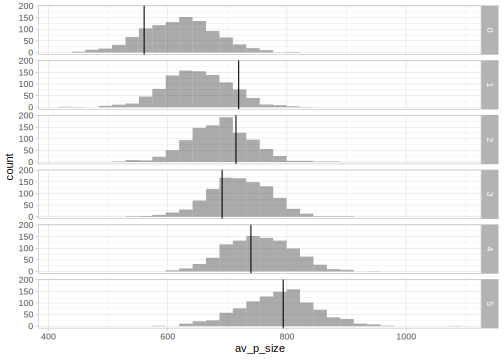
\includegraphics{bookdown_files/figure-latex/postpredmean-1.pdf}
\caption{\label{fig:postpredmean}Distribution of posterior predicted means in gray and observed pupil size means in black lines by load.}
\end{figure}

Figure \ref{fig:postpredmean} shows that the observed means for no load and for a load of two are falling in the tails of the distributions. While our model predicts a monotonic increase of pupil size, the data might be indicating that the relevant difference is between (i) no load, (ii) a load between two and three, and then (iii) a load of four, and (iv) of five. However, given the uncertainty in the posterior predictive distributions and that the observed means are contained somewhere in the predicted distributions, it could be the case that we are overinterpreting noise.

\hypertarget{sec:trial}{%
\section{Log-normal model: Does trial affect pupil size?}\label{sec:trial}}

Let us revisit the small experiment from section \ref{sec:simplenormal}, where a participant repeatedly pressed the space bar as fast as possible, without paying attention to the stimuli. We want to know whether the participant tended to speedup (practice effect) or slowdown (fatigue effect) while pressing the space bar.

\hypertarget{likelihood-and-priors-for-the-log-normal-model}{%
\subsection{Likelihood and priors for the log-normal model}\label{likelihood-and-priors-for-the-log-normal-model}}

If we assume that reaction times are log-normally distributed, we could fit a likelihood such as the following:

\begin{equation}
rt_n \sim LogNormal(\alpha + c\_trial_n \cdot \beta,\sigma)
\label{eq:rtloglik}
\end{equation}

where \(n =1, \ldots, N\), and \(rt\) is the dependent variable (reaction times in milliseconds). The variable \(N\) represents the total number of data points.

We use the same priors as in section \ref{sec:lognormal} for \(\alpha\) (which is equivalent to \(\mu\) in the previous model) and for \(\sigma\).

\begin{equation}
\begin{aligned}
\alpha &\sim Normal(6, 1.5) \\
\sigma &\sim Normal_+(0, 1)\\
\end{aligned}
\end{equation}

We still need a prior for \(\beta\), but notice that effects are multiplicative rather than additive when we assume a log-normal likelihood and that means that we need to take into account \(\alpha\) in order to interpret \(\beta\); see Box \ref{thm:lognormal}. We are going to try to understand how all our priors interact together generating some prior predictive distributions. We start with the following prior centered in zero, a prior agnostic regarding the direction of the effect, which allows for both a slowdowns (\(\beta>0\)) or a speedups (\(\beta<0\)):

\begin{equation}
\beta \sim Normal(0, 1)
\end{equation}

We can edit our \texttt{normal\_predictive\_distribution\_fast} from section \ref{sec:ppd} and make it log-normal and dependent on trial:

\begin{Shaded}
\begin{Highlighting}[]
\NormalTok{lognormal_model_pred <-}\StringTok{ }\ControlFlowTok{function}\NormalTok{(alpha_samples,}
\NormalTok{                                 beta_samples,}
\NormalTok{                                 sigma_samples,}
\NormalTok{                                 N_obs) \{}
    \CommentTok{# pmap extends map2 (and map) for a list of lists:}
    \KeywordTok{pmap_dfr}\NormalTok{(}\KeywordTok{list}\NormalTok{(alpha_samples, beta_samples, sigma_samples),}
             \ControlFlowTok{function}\NormalTok{(alpha, beta, sigma) \{}
                 \KeywordTok{tibble}\NormalTok{(}
                     \DataTypeTok{trialn =} \KeywordTok{seq_len}\NormalTok{(N_obs),}
                     \CommentTok{# we center trial:}
                     \DataTypeTok{c_trial =}\NormalTok{ trialn }\OperatorTok{-}\StringTok{ }\KeywordTok{mean}\NormalTok{(trialn),}
                     \CommentTok{# we change the likelihood: }
                     \CommentTok{# Notice rlnorm and the use of alpha and beta}
                     \DataTypeTok{rt_pred =} \KeywordTok{rlnorm}\NormalTok{(N_obs, alpha }\OperatorTok{+}\StringTok{ }\NormalTok{c_trial }\OperatorTok{*}\StringTok{ }\NormalTok{beta, sigma)}
\NormalTok{                 )}
\NormalTok{             \}, }\DataTypeTok{.id =} \StringTok{"iter"}\NormalTok{) }\OperatorTok
\StringTok{    }\CommentTok{# .id is always a string and needs to be converted to a number}
\StringTok{        }\KeywordTok{mutate}\NormalTok{(}\DataTypeTok{iter =} \KeywordTok{as.numeric}\NormalTok{(iter))}
\NormalTok{\}}
\end{Highlighting}
\end{Shaded}

This is our first attempt for a prior predictive distribution:

\begin{Shaded}
\begin{Highlighting}[]
\NormalTok{N_obs =}\StringTok{ }\DecValTok{361}
\NormalTok{alpha_samples <-}\StringTok{ }\KeywordTok{rnorm}\NormalTok{(}\DecValTok{1000}\NormalTok{, }\DecValTok{6}\NormalTok{, }\FloatTok{1.5}\NormalTok{)}
\NormalTok{sigma_samples <-}\StringTok{ }\KeywordTok{rtnorm}\NormalTok{(}\DecValTok{1000}\NormalTok{, }\DecValTok{0}\NormalTok{, }\DecValTok{1}\NormalTok{, }\DataTypeTok{a =}\DecValTok{0}\NormalTok{)}
\NormalTok{beta_samples <-}\StringTok{ }\KeywordTok{rnorm}\NormalTok{(}\DecValTok{1000}\NormalTok{, }\DecValTok{0}\NormalTok{, }\DecValTok{1}\NormalTok{)}

\NormalTok{prior_pred <-}\StringTok{ }\KeywordTok{lognormal_model_pred}\NormalTok{(}
    \DataTypeTok{alpha_samples =}\NormalTok{ alpha_samples,}
    \DataTypeTok{beta_samples =}\NormalTok{ beta_samples, }
    \DataTypeTok{sigma_samples =}\NormalTok{ sigma_samples,}
    \DataTypeTok{N_obs =}\NormalTok{ N_obs)}
\end{Highlighting}
\end{Shaded}

We look here at the median effect:

\begin{Shaded}
\begin{Highlighting}[]
\NormalTok{median_effect <-}
\StringTok{     }\NormalTok{prior_pred }\OperatorTok
\StringTok{     }\KeywordTok{group_by}\NormalTok{(iter) }\OperatorTok
\StringTok{     }\KeywordTok{mutate}\NormalTok{(}\DataTypeTok{diff =}\NormalTok{ rt_pred }\OperatorTok{-}\StringTok{ }\KeywordTok{lag}\NormalTok{(rt_pred)) }\OperatorTok
\StringTok{     }\KeywordTok{summarize}\NormalTok{(}
         \DataTypeTok{median_rt =} \KeywordTok{median}\NormalTok{(diff, }\DataTypeTok{na.rm =} \OtherTok{TRUE}\NormalTok{)}
\NormalTok{ )}
\end{Highlighting}
\end{Shaded}

We plot it in Figure \ref{fig:priorbeta}, and as expected is center in zero (as our prior), but we see that the distribution of possible medians for the effect is too spread and includes values that are too extreme.



\begin{Shaded}
\begin{Highlighting}[]
\NormalTok{median_effect }\OperatorTok
\StringTok{    }\KeywordTok{ggplot}\NormalTok{(}\KeywordTok{aes}\NormalTok{(median_rt)) }\OperatorTok{+}
\StringTok{    }\KeywordTok{geom_histogram}\NormalTok{()}
\end{Highlighting}
\end{Shaded}

\begin{figure}
\centering
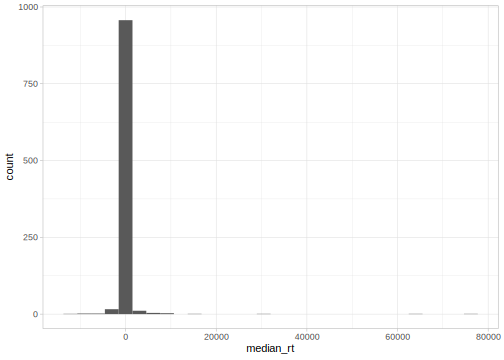
\includegraphics{bookdown_files/figure-latex/priorbeta-1.pdf}
\caption{\label{fig:priorbeta}Prior predictive distribution of the median effect of the model defined in \ref{sec:trial} with \(\beta \sim Normal(0, 1)\).}
\end{figure}

We repeat the same procedure with \(\beta \sim Normal(0,.01)\), and we plot it in Figure \ref{fig:priorbeta2}. The prior predictive distribution shows us that the prior is still quite vague, it is, howeverm at least in the right order of magnitude. Notice that we are using a distribution of medians because they are less affected by the variance in the posterior predicted distribution; distributions of means will have much more spread. If we want to make the distribution of means more realistic, we would also need to find a more accurate prior for the scale, \(\sigma\).



\begin{figure}
\centering
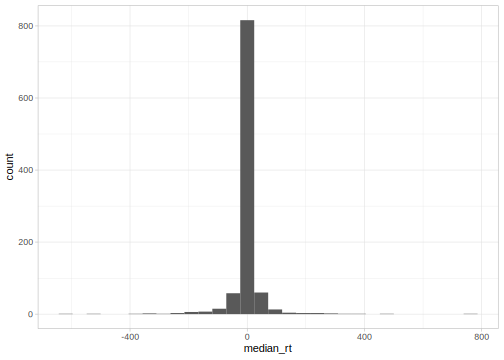
\includegraphics{bookdown_files/figure-latex/priorbeta2-1.pdf}
\caption{\label{fig:priorbeta2}Prior predictive distribution of the median effect of the model defined in \ref{sec:trial} with \(\beta \sim Normal(0, .01)\).}
\end{figure}

Prior selection might look daunting and a lot of work. However, this work is usually done only the first time we encounter an experimental paradigm; besides, priors can be informed by the estimates from previous experiments (even maximum likelihood estimates from frequentist models can be useful). We will generally use very similar (or identical priors) for analyses dealing with the same type of task. When in doubt, a sensitivity analysis (see section \ref{sec:sensitivity}) can tell us whether the posterior distribution depends unintentionally strongly on our prior selection.

\Begin{extra}

\BeginKnitrBlock{theorem}
\protect\hypertarget{thm:lognormal}{}{\label{thm:lognormal} }\textbf{Understanding the Log-normal likelihood}
\EndKnitrBlock{theorem}

It is important to understand what we are assuming with our log-normal likelihood. Formally, if a random variable \(Y\) is normally distributed with mean \(\mu\) and variance \(\sigma^2\), then the transformed random variable \(V = \exp(Y)\) is log-normally distributed and has density:

\begin{equation}
LogNormal(v|\mu,\sigma)=f(y)= \frac{1}{\sqrt{2\pi \sigma^2}v} \exp \left(-\frac{(\log(v)-\mu)^2}{2\sigma^2} \right)
\end{equation}

As explained in section \ref{sec:lnfirst}, the model from \eqref{eq:rtloglik} is equivalent to the following:

\begin{equation}
\log(rt_n) \sim Normal(\alpha + c\_trial_n \cdot \beta,\sigma)\\
\end{equation}

This, in turn, can be written as follows (see ??):

\begin{equation}
\log(rt_n) \sim Normal(\alpha, \sigma) + c\_trial_n \cdot \beta
\label{eq:rtlogliknoncen}
\end{equation}

We exponentiate both sides, and we use the property of exponents that \(\exp(x+y)\) is equivalent to \(\exp(x) \cdot exp(y)\).
\begin{equation}
\begin{aligned}
rt_n &\sim \exp \big(Normal(\alpha, \sigma)  + c\_trial_n \cdot \beta\big) \\
rt_n &\sim \exp\big(Normal(\alpha, \sigma)\big)   \cdot \exp\big(c\_trial_n \cdot \beta\big) \\
rt_n &\sim LogNormal(\alpha, \sigma)   \cdot \exp\big(c\_trial_n \cdot \beta\big) 
\end{aligned}
\end{equation}

So, essentially, we are assuming that reaction times are log-normally distributed with a median of \(\exp(\alpha)\) and that the effect of trial number is multiplicative and grows or decays exponentially with the trial number. This has two important consequences:

\begin{enumerate}
\def\labelenumi{\arabic{enumi}.}
\item
  Different values of the intercept, \(\alpha\), given the same \(\beta\), will affect the difference in reaction times for two adjacent trials (this is contrast to what happens with an additive model such as normal likelihood); see Figure \ref{fig:logexp}. This is because, unlike in the additive case, the intercept doesn't cancel out:

  \begin{itemize}
  \item
    Additive case:

    \begin{equation}
    \begin{aligned}
    & (\alpha + trial_n \cdot \beta) - (\alpha + trial_{n-1} \cdot \beta) = \\
    &=\alpha -\alpha + ( trial_n - trial_{n-1} ) \cdot \beta\\
    &= ( trial_n - trial_{n-1} ) \cdot \beta
    \end{aligned}
    \end{equation}
  \item
    Multiplicative case:

    \begin{equation}
    \begin{aligned}
       &\exp(\alpha) \cdot \exp(trial_n \cdot \beta) -\exp(\alpha) \cdot \exp(trial_{n-1} \cdot \beta) =\\ 
       &= \exp(\alpha) \big(\exp(trial_n  \cdot \beta)  - \exp(trial_{n-1}\cdot \beta) \big)\\
       &= \exp(\alpha) \big(\exp(trial_n)  - \exp(trial_{n-1}  \big) \cdot \exp(\beta)\\
       &\neq \big(\exp(trial_n)  - \exp(trial_{n-1}  \big) \cdot \exp(\beta) 
    \end{aligned}
       \end{equation}
  \end{itemize}
\end{enumerate}



\begin{figure}[H]
  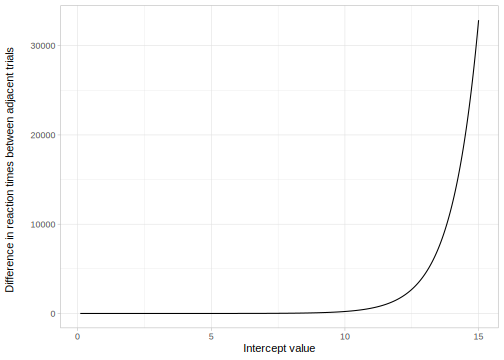
\includegraphics{bookdown_files/figure-latex/logexp-1} \caption{Fitted value of the difference in reaction time between two adjacent trials, when \(\beta=0.01\) and \(\alpha\) lies between 0.1 and 15. The graph shows how changes in the intercept lead to changes in the difference in reaction times between trials, even if \(\beta\) is fixed.}\label{fig:logexp}
  \end{figure}

\begin{enumerate}
\def\labelenumi{\arabic{enumi}.}
\setcounter{enumi}{1}
\tightlist
\item
  As the trial number increases, the same value of \(\beta\) will have a very different impact on the original scale of the dependent variable: \(\beta <0\) will lead to exponential decay and \(\beta >0\) will lead to exponential growth; see figure \ref{fig:expgd}.
\end{enumerate}



\begin{figure}[H]
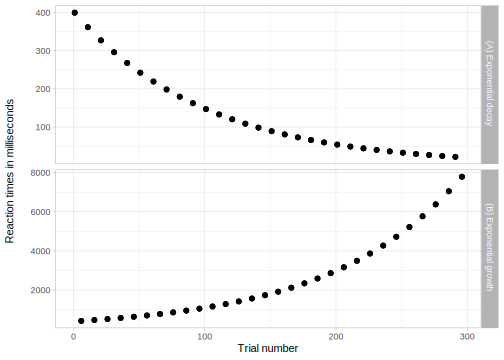
\includegraphics{bookdown_files/figure-latex/expgd-1} \caption{Fitted value of the dependent variable (reaction times in ms) as function of trial number, when (A) \(\beta = -0.01\), exponential decay, and when (B) \(\beta =.01\), exponential growth.}\label{fig:expgd}
\end{figure}

Can exponential growth or decay make sense? We need to consider if they do make sense, they will be an approximation valid for a specific range of values, at some point we will expect a ceiling effect: reaction times cannot truly be 0 milliseconds, or take minutes. However, in our specific model, exponential growth or decay \emph{by trial} is probably a bad approximation: We will predict that our participant will take extremely long (if \(\beta >0\)) or extremely short (if \(\beta <0\)) time in pressing the space bar in a relatively low number of trials. This doesn't mean that the likelihood is wrong by itself, but it does mean that at least we need to put a cap on the growth or decay of our experimental manipulation. We can do this if the exponential growth or decay is a function of, for example, log-transformed trial numbers:

\begin{equation}
rt_n \sim LogNormal(\alpha + \log(c\_trial_n) \cdot \beta,\sigma)\\
\end{equation}



\begin{figure}[H]
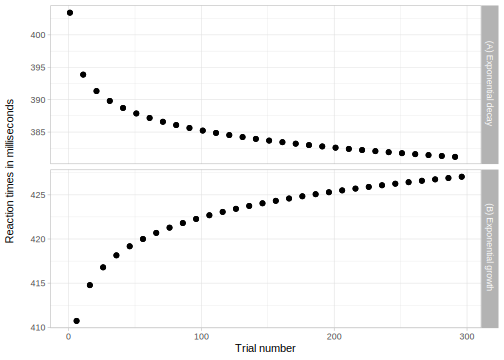
\includegraphics{bookdown_files/figure-latex/expgd2-1} \caption{Fitted value of the dependent variable (reaction times in ms) as function of the natural logarithm of the trial number, when (A) \(\beta=-0.01\), exponential decay, and when (B) \(\beta =.01\), exponential growth.}\label{fig:expgd2}
\end{figure}

\textbf{Log-normal distributions all the way down}

The normal distribution is most often assumed to describe the random variation that occurs in the data from many scientific disciplines. However, most measurements actually show skewed distributions. \citet{limpertLognormalDistributionsSciences2001} discuss the log-normal distribution in scientific disciplines and how diverse type of data, from lengths of latent periods of infectious diseases to distribution of mineral resources in the Earth's crust, including even body height--the quintessential example of a normal distribution--, closely fit the log-normal distribution.

\citet{limpertLognormalDistributionsSciences2001} point out that because a random variable that results from multiplicating many independent variables has an approximate log-normal distribution, the most basic indicator of the importance of the log-normal distribution may be very general: Chemistry and physics are fundamental in life, and the prevailing operation in the laws of these disciplines is multiplication rather than addition.

Furthermore, at many physiological and anatomical levels in the brain, the distribution of numerous parameters is in fact strongly skewed with a heavy tail, suggesting that skewed (typically log-normal) distributions are fundamental to structural and functional brain organization. This might be explained given that the majority of interactions in highly interconnected systems, especially in biological systems, are multiplicative and synergistic rather than additive \citep{buzsakiLogdynamicBrainHow2014}.

Does the log-normal distribution make sense for reaction times?
It has been long noticed that log-normal distribution often provides a good fit to reaction times
distributions \citep{ref}.
One advantage of assuming log-normally distributed reaction times (but, in fact, this is true for many skewed distributions), is that it entails that the standard deviation of the reaction time distribution will increases with the mean, as has been observed in empirical distributions of reaction times \citep{wagenmakersRelationMeanVariance2005}. Interestingly, it turns out that log-normal reaction times are also easily generated by certain process models. \citet{ulrichInformationProcessingModels1993} shows, for example, that models in which reaction times are determined by a series of processes cascading activation from an input level to an output level (usually passing through a number of intervening processing levels along the way) can generate log-normally distributed reaction times.

\End{extra}

\hypertarget{the-brms-model-1}{%
\subsection{\texorpdfstring{The \texttt{brms} model}{The brms model}}\label{the-brms-model-1}}

We are now relatively satisfied with the priors for our model, and we can fit the data with \texttt{brms}. Notice that we need to specify that the family is \texttt{lognormal()}.

\begin{Shaded}
\begin{Highlighting}[]
\NormalTok{df_noreading_data <-}\StringTok{ }\KeywordTok{read_csv}\NormalTok{(}\StringTok{"./data/button_press.csv"}\NormalTok{)}
\NormalTok{df_noreading_data <-}\StringTok{ }\NormalTok{df_noreading_data }\OperatorTok
\StringTok{    }\KeywordTok{mutate}\NormalTok{(}\DataTypeTok{c_trial =}\NormalTok{ trialn }\OperatorTok{-}\StringTok{ }\KeywordTok{mean}\NormalTok{(trialn))}

\NormalTok{fit_press_trial <-}\StringTok{ }\KeywordTok{brm}\NormalTok{(rt }\OperatorTok{~}\StringTok{ }\DecValTok{1} \OperatorTok{+}\StringTok{ }\NormalTok{c_trial,}
  \DataTypeTok{data =}\NormalTok{ df_noreading_data,}
  \DataTypeTok{family =} \KeywordTok{lognormal}\NormalTok{(),}
  \DataTypeTok{prior =} \KeywordTok{c}\NormalTok{(}
    \KeywordTok{prior}\NormalTok{(}\KeywordTok{normal}\NormalTok{(}\DecValTok{6}\NormalTok{, }\FloatTok{1.5}\NormalTok{), }\DataTypeTok{class =}\NormalTok{ Intercept),}
    \KeywordTok{prior}\NormalTok{(}\KeywordTok{normal}\NormalTok{(}\DecValTok{0}\NormalTok{, }\DecValTok{1}\NormalTok{), }\DataTypeTok{class =}\NormalTok{ sigma),}
    \KeywordTok{prior}\NormalTok{(}\KeywordTok{normal}\NormalTok{(}\DecValTok{0}\NormalTok{, }\DecValTok{1}\NormalTok{), }\DataTypeTok{class =}\NormalTok{ b, }\DataTypeTok{coef =}\NormalTok{ c_trial)}
\NormalTok{  )}
\NormalTok{)}
\end{Highlighting}
\end{Shaded}

Instead of printing out the complete output from the model, look at the estimates from the posteriors for the parameters \(\alpha\), \(\beta\), and \(\sigma\). Notice that these parameters are on the log scale:

\begin{Shaded}
\begin{Highlighting}[]
\CommentTok{## print posterior means and 95% credible intervals to four decimal places:}
\KeywordTok{posterior_summary}\NormalTok{(fit_press_trial)[}\DecValTok{1}\OperatorTok{:}\DecValTok{3}\NormalTok{,}\KeywordTok{c}\NormalTok{(}\DecValTok{1}\NormalTok{,}\DecValTok{3}\NormalTok{,}\DecValTok{4}\NormalTok{)]}
\end{Highlighting}
\end{Shaded}

\begin{verbatim}
##             Estimate   Q2.5   Q97.5
## b_Intercept  5.11824 5.1053 5.13100
## b_c_trial    0.00052 0.0004 0.00065
## sigma        0.12323 0.1143 0.13336
\end{verbatim}

The posterior distributions can be plotted to obtain a graphical summary of all the parameters in the model:

\begin{Shaded}
\begin{Highlighting}[]
\KeywordTok{plot}\NormalTok{(fit_press_trial)}
\end{Highlighting}
\end{Shaded}

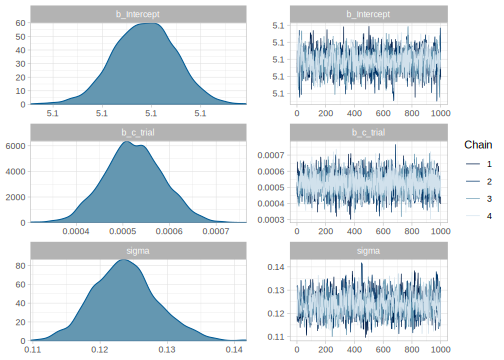
\includegraphics{bookdown_files/figure-latex/unnamed-chunk-97-1.pdf}

Next, we turn to the question of what we can report as our results, and what we can conclude from the data.

\hypertarget{how-to-communicate-the-results-1}{%
\subsection{How to communicate the results?}\label{how-to-communicate-the-results-1}}

As shown above, the first step is to summarize the posteriors in a table or graphically (or both). If the research relates to the effect estimated by the model, the posterior of \(\beta\) can be summarized in the following way: \(\hat\beta = 0.00052\), 95\% CrI = \([ 0.0004 , 0.00065 ]\).

But in most cases, the effect is easier to interpret in milliseconds. We can transform the estimates back to the millisecond scale from the log scale, but we need to take into account that the scale is not linear, and that the effect between two button presses will differ depending on where we are in the experiment.

We will have a different estimate if we consider the difference between reaction times in a trial at the middle of the experiment (when the centered trial number is zero) and the previous one (when the centered trial number is minus one).

\begin{Shaded}
\begin{Highlighting}[]
\NormalTok{alpha_samples<-}\StringTok{ }\KeywordTok{posterior_samples}\NormalTok{(fit_press_trial)}\OperatorTok{$}\NormalTok{b_Intercept}
\NormalTok{beta_samples<-}\StringTok{ }\KeywordTok{posterior_samples}\NormalTok{(fit_press_trial)}\OperatorTok{$}\NormalTok{b_c_trial}
\NormalTok{effect_middle_ms <-}\StringTok{ }\KeywordTok{exp}\NormalTok{(alpha_samples) }\OperatorTok{-}\StringTok{ }\KeywordTok{exp}\NormalTok{(alpha_samples }\OperatorTok{-}\StringTok{ }\DecValTok{1}\OperatorTok{*}\StringTok{ }\NormalTok{beta_samples)}
\CommentTok{## ms effect in the middle of the expt (mean trial vs. mean trial - 1 ) }
\KeywordTok{c}\NormalTok{(}\DataTypeTok{mean =} \KeywordTok{mean}\NormalTok{(effect_middle_ms), }\KeywordTok{quantile}\NormalTok{(effect_middle_ms, }\KeywordTok{c}\NormalTok{(.}\DecValTok{025}\NormalTok{,.}\DecValTok{975}\NormalTok{)))}
\end{Highlighting}
\end{Shaded}

\begin{verbatim}
##  mean  2.5%   98% 
## 0.088 0.066 0.109
\end{verbatim}

than if we consider the difference between the second trial and the first one:

\begin{Shaded}
\begin{Highlighting}[]
\NormalTok{first_trial <-}\StringTok{ }\KeywordTok{min}\NormalTok{(df_noreading_data}\OperatorTok{$}\NormalTok{c_trial)}
\NormalTok{second_trial <-}\StringTok{ }\KeywordTok{min}\NormalTok{(df_noreading_data}\OperatorTok{$}\NormalTok{c_trial) }\OperatorTok{+}\DecValTok{1}
\NormalTok{effect_beginning_ms <-}\StringTok{ }\KeywordTok{exp}\NormalTok{(alpha_samples}\OperatorTok{+}\StringTok{  }\NormalTok{second_trial }\OperatorTok{*}\StringTok{ }\NormalTok{beta_samples) }\OperatorTok{-}
\StringTok{    }\KeywordTok{exp}\NormalTok{(alpha_samples}\OperatorTok{+}\StringTok{  }\NormalTok{first_trial }\OperatorTok{*}\StringTok{ }\NormalTok{beta_samples)}
\CommentTok{## ms effect from first to second trial:}
\KeywordTok{c}\NormalTok{(}\DataTypeTok{mean =} \KeywordTok{mean}\NormalTok{(effect_beginning_ms), }\KeywordTok{quantile}\NormalTok{(effect_beginning_ms, }\KeywordTok{c}\NormalTok{(.}\DecValTok{025}\NormalTok{,.}\DecValTok{975}\NormalTok{)))}
\end{Highlighting}
\end{Shaded}

\begin{verbatim}
##  mean  2.5%   98% 
## 0.080 0.062 0.097
\end{verbatim}

There is a slowdown in both cases; when reporting the results of these analyses, one could present the posterior mean and the 95\% credible interval and then reason about whether the observed estimates are consistent with the prediction from the theory being investigated.

The practical relevance of the effect for the research question can be important too. For example, only after 100 button presses do we see a slowdown of 9 ms on average (\(0.09 \cdot 100\)), with a 95\% credible interval ranging from 6.62 to 10.88. We need to consider whether our uncertainty of this estimate, and the estimated mean effect have any scientific relevance. Such relevance can be established by considering the previous literature, predictions from a quantitative model, or other expert domain knowledge. Sometimes, a quantitative meta-analysis is helpful; for examples, see \citet{JaegerEngelmannVasishth2017},\citet{mahowald2016meta},\citet{NicenboimRoettgeretal}, and \citet{vasishthProcessingChineseRelative2013}. We will discuss concrete examples later in the book, in section ??.

Sometimes, researchers are only interested in establishing that there is an effect; the magnitude and uncertainty of the estimate is of secondary interest. Here, the goal is to argue that there is \textbf{evidence} of a slowdown. The word evidence has a special meaning in statistics \citep{Royall}, and in null hypothesis significance testing, a likelihood ratio test is the standard way to argue that one has evidence for an effect. In the Bayesian data analysis context, a Bayes factor hypothesis test must be carried out. We'll come back to this issue in the model comparison section @ref(sec:?).

\hypertarget{sec:logistic}{%
\section{Logistic regression: Does set size affect free recall?}\label{sec:logistic}}

We'll look at the capacity limit of working memory to illustrate how the principles we have learned so far can naturally extend to \emph{generalized} linear models (GLMs). In this section, we focus on one special case of GLMS, logistic regression.

For this example, we'll use a subset of the data of \citet{oberauerWorkingMemoryCapacity2019}. We'll focus on one subject who was presented word lists of varying lengths (2, 4, 6, and 8 elements), and then was asked to recall a word given its position on the list; see Figure \ref{fig:oberauer}.\footnote{We will only use data from the recall test in which the participant had to type the probed word (and we will ignore the trials with multiple forced choice for ease of explanation).}



\begin{figure}
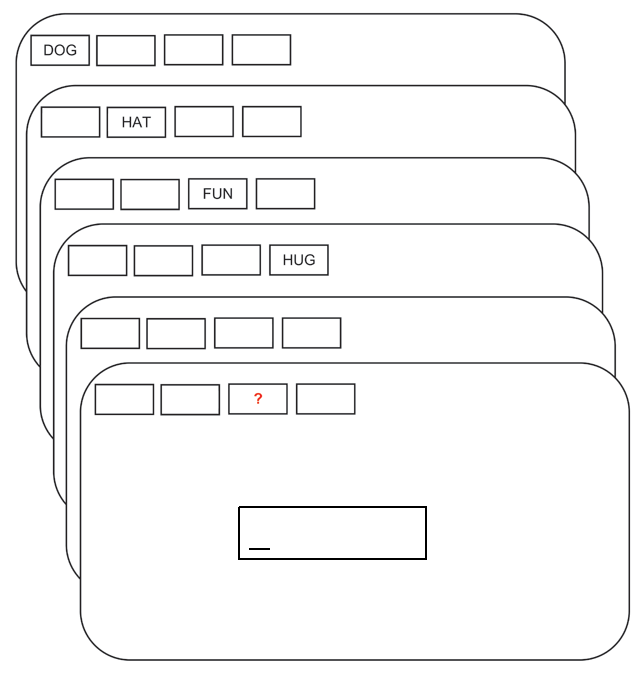
\includegraphics[width=8.89in]{cc_figure/fig1_oberauer_2019_modified} \caption{Flow of events in a trial with memory set size 4 and free recall. Adapted from \citet{oberauerWorkingMemoryCapacity2019}; licensed under CC BY 4.0.}\label{fig:oberauer}
\end{figure}

It is well established that as the number of items to be held in working memory increases, performance, that is accuracy, decreases \citep[among others][]{oberauerkliegel2001}. We will investigate whether we can establish this finding with data from only one subject.

\begin{Shaded}
\begin{Highlighting}[]
\NormalTok{df_recall_data <-}\StringTok{ }\KeywordTok{read_table2}\NormalTok{(}\StringTok{"./data/PairsRSS1_all.dat"}\NormalTok{,}
                              \DataTypeTok{col_names =} \KeywordTok{c}\NormalTok{(}\StringTok{"subject"}\NormalTok{, }\StringTok{"session"}\NormalTok{, }\StringTok{"block"}\NormalTok{,}
                                            \StringTok{"trial"}\NormalTok{, }\StringTok{"set_size"}\NormalTok{,}
                                            \StringTok{"response_size_list"}\NormalTok{,}
                                            \StringTok{"response_size_new_words"}\NormalTok{,}
                                            \StringTok{"tested"}\NormalTok{, }\StringTok{"response"}\NormalTok{,}
                                            \StringTok{"response_category"}\NormalTok{, }\StringTok{"rt"}\NormalTok{)) }\OperatorTok
\StringTok{    }\CommentTok{# We ignore the type of incorrect responses (the focus of the paper)}
\StringTok{    }\KeywordTok{mutate}\NormalTok{(}\DataTypeTok{correct =} \KeywordTok{if_else}\NormalTok{(response_category }\OperatorTok{==}\DecValTok{1}\NormalTok{, }\DecValTok{1}\NormalTok{, }\DecValTok{0}\NormalTok{)) }\OperatorTok
\StringTok{    }\CommentTok{# and we only use the data from the free recall task:}
\StringTok{    }\CommentTok{# (when there was no list of possible responses)}
\StringTok{    }\KeywordTok{filter}\NormalTok{(response_size_list }\OperatorTok{+}\StringTok{ }\NormalTok{response_size_new_words }\OperatorTok{==}\StringTok{ }\DecValTok{0}\NormalTok{) }\OperatorTok
\StringTok{    }\CommentTok{# We select one subject}
\StringTok{    }\KeywordTok{filter}\NormalTok{(subject }\OperatorTok{==}\StringTok{ }\DecValTok{10}\NormalTok{) }\OperatorTok
\StringTok{    }\KeywordTok{mutate}\NormalTok{(}\DataTypeTok{c_set_size =}\NormalTok{ set_size }\OperatorTok{-}\StringTok{ }\KeywordTok{mean}\NormalTok{(set_size))}
\CommentTok{# we can ignore the warning from read_table}

\CommentTok{# Set sizes in the dataset:}
\NormalTok{df_recall_data}\OperatorTok{$}\NormalTok{set_size }\OperatorTok
\StringTok{    }\NormalTok{unique}
\end{Highlighting}
\end{Shaded}

\begin{verbatim}
## [1] 4 8 2 6
\end{verbatim}

\begin{Shaded}
\begin{Highlighting}[]
\CommentTok{# Trials by set size}
\NormalTok{df_recall_data }\OperatorTok
\StringTok{    }\KeywordTok{group_by}\NormalTok{(set_size) }\OperatorTok
\StringTok{    }\KeywordTok{count}\NormalTok{()}
\end{Highlighting}
\end{Shaded}

\begin{verbatim}
## # A tibble: 4 x 2
## # Groups:   set_size [4]
##   set_size     n
##      <dbl> <int>
## 1        2    23
## 2        4    23
## 3        6    23
## 4        8    23
\end{verbatim}

The data look like this: the column \texttt{correct} records the 0 (incorrect) or 1 (correct) responses, and the column \texttt{c\textbackslash{}\_set\textbackslash{}\_size} records the centered memory set size; these latter scores have continuous values -3, -1, 1, and 3. These continuous values are centered versions of 2, 4, 6, and 8.

\begin{Shaded}
\begin{Highlighting}[]
\NormalTok{df_recall_data<-df_recall_data[,}\KeywordTok{c}\NormalTok{(}\DecValTok{12}\NormalTok{,}\DecValTok{13}\NormalTok{)]}
\NormalTok{df_recall_data}
\end{Highlighting}
\end{Shaded}

\begin{verbatim}
## # A tibble: 92 x 2
##   correct c_set_size
##     <dbl>      <dbl>
## 1       1         -1
## 2       0          3
## 3       1         -3
## 4       1          1
## 5       1         -1
## # ... with 87 more rows
\end{verbatim}

We want to model the trial by trial accuracy and examine whether the probability of recalling a word is related to the number of words in the set that the subject needs to remember.

\hypertarget{the-likelihood-for-the-logistic-regression-model}{%
\subsection{The likelihood for the logistic regression model}\label{the-likelihood-for-the-logistic-regression-model}}

Recall that the Bernoulli likelihood generates a 0 or 1 response with a particular probability \(\theta\). For example, one can generate simulated data for 10 trials as follows:

\begin{Shaded}
\begin{Highlighting}[]
\KeywordTok{as.numeric}\NormalTok{(}\KeywordTok{rbernoulli}\NormalTok{(}\DataTypeTok{n=}\DecValTok{10}\NormalTok{,}\DataTypeTok{p=}\FloatTok{0.5}\NormalTok{))}
\end{Highlighting}
\end{Shaded}

\begin{verbatim}
##  [1] 1 0 0 0 1 0 0 0 0 0
\end{verbatim}

We can therefore define each dependent value correct\_n in the data as being generated from a Bernoulli random variable with probability of success \(\theta_n\).
Here, \(n =1, \ldots, N\) indexes the trial, correct\_n is the dependent variable (0 indicates an incorrect recall and 1 a correct recall), and \(\theta_n\) is the probability of correctly recalling a probe in a given trial \(n\).

\begin{equation}
correct_n \sim Bernoulli(\theta_n)
\label{eq:bernoullilik}
\end{equation}

Since \(\theta_n\) is bounded to be between 0 and 1 (it is a probability), we cannot just fit a regression model using the normal or lognormal likelihood as we did in the preceding examples. Such a model would be inappropriate because it would assume that the data range from \(-\infty\) to \(+\infty\), but in fact the probabilities we want to estimate lie within the {[}0,1{]} boundary.

The generalized linear modeling framework solves this problem by defining a so-called \textbf{link function} \(g(\cdot)\) that connects the linear model to the quantity to be estimated (here, the probabilities \(\theta_n\)). The link function used for 0,1 responses is called the \textbf{logit link}, and is defined as follows.

\begin{equation}
\eta_n = g(\theta_n) = \log\left(\frac{\theta_n}{1-\theta_n}\right)
\end{equation}

The term \(\frac{\theta_n}{1-\theta_n}\) is called the \textbf{odds}.\footnote{Odds are defined to be the ratio of the probability of success to the probability of failure. For example, the odds of obtaining a one in a fair six-sided die are \(\frac{1/6}{1-1/6}=1/5\). The odds of obtaining a heads in a fair coin are 1/1.} The logit link function is therefore a log-odds; it maps real numbers ranging from \((-\infty,+\infty)\) to probability values ranging from \([0,1]\). Figure \ref{fig:logisticfun} shows the logit link function, \(\eta = g(\theta)\), and the inverse logit, \(\theta = g^{-1}(\eta)\), which is called the \textbf{logistic function}; the relevance of this logistic function will become clear in a moment.

\begin{figure}
\centering
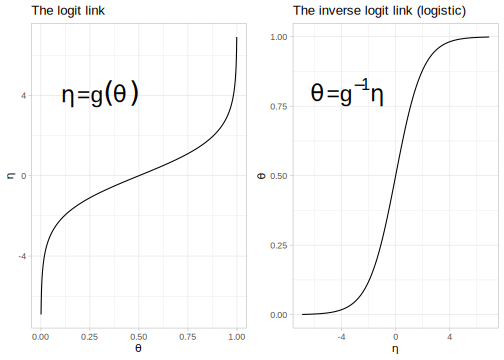
\includegraphics{bookdown_files/figure-latex/logisticfun-1.pdf}
\caption{\label{fig:logisticfun}The logit and inverse logit (logistic) function.}
\end{figure}

The linear model is now fit not to the 0,1 responses as the dependent variable, but to \(\eta_n\), i.e., log-odds, as the dependent variable:

\begin{equation}
\eta_n = \log\left(\frac{\theta_n}{1-\theta_n}\right) = \alpha + \beta \cdot c\_set\_size
\end{equation}

Once \(\eta_n\) is estimated, one can easily compute the parameters of interest, the estimated probabilities, by solving the above equation for \(\theta_n\) (in other words, by computing the inverse of the logit function), which is the above-mentioned logistic regression function:

\begin{equation}
\theta_n = g^{-1}(\eta_n) =  \log\left(\frac{\exp(\eta_n)}{1+\exp(\eta_n)}\right)
\end{equation}

In summary, the generalized linear model with the logit link fits the following Bernoulli likelihood:

\begin{equation}
correct_n \sim Bernoulli(\theta_n)
\label{eq:bernoullilogislik}
\end{equation}

The model is fit on the log-odds scale, \(\eta_n = \alpha + c\_set\_size_n \cdot \beta\).
Once \(\eta_n\) has been estimated, the inverse logit or the logistic function is used to compute the probability estimates
\(\theta_n = \log(\frac{\exp(\eta_n)}{1+\exp(\eta_n)})\)`. An example of the calculations will be shown in the next section.

\hypertarget{priors-for-logistic-regression}{%
\subsection{Priors for logistic regression}\label{priors-for-logistic-regression}}

In order to decide on priors for \(\alpha\) and \(\beta\) we need to take into account that these parameter do not represent probabilities or proportions, but \emph{log-odds}, the x-axis in Figure \ref{fig:logisticfun} (right-hand side figure). As shown in the figure, the relationship between log-odds and probabilities is not linear.

There are two functions in R that implement the logit and inverse logit functions: \texttt{qlogis(p)} for the logit function and \texttt{plogis(x)} for the inverse logit or logistic function.

Now we need to set priors for \(\alpha\) and \(\beta\).
Given that we centered our predictor, the intercept, \(\alpha\), represents the probability of correctly recalling one word in a random position for the average set size of five (since \(5 = \frac{2+4+6+8}{4}\)), which, incidentally, was not presented in the experiment. This is one case where the intercept doesn't have a clear interpretation if we leave the prediction uncentered: With non-centered set size, the intercept will be the probability of recalling one word in a set of \emph{zero} words.

The prior for \(\alpha\) will depend on how difficult the recall task is. If we are not sure, we could assume that the probability of recalling a word for an average set size, \(\alpha\), is centered in .5 (a 50/50 chance) with a great deal of uncertainty. The \texttt{R} command \texttt{plogis(.5)} tells us that .5 corresponds to zero in log-odds. How do we include a great deal of uncertainty? We could look at Figure \ref{fig:logisticfun}, and decide on a standard deviation of 4 in a normal distribution centered in zero:

\begin{equation}
\alpha \sim Normal(0, 4) 
\end{equation}

Let's plot this prior in log-odds and in probability scale by drawing random samples.



\begin{Shaded}
\begin{Highlighting}[]
\NormalTok{samples_logodds <-}\StringTok{ }\KeywordTok{tibble}\NormalTok{(}\DataTypeTok{alpha =} \KeywordTok{rnorm}\NormalTok{(}\DecValTok{100000}\NormalTok{, }\DecValTok{0}\NormalTok{, }\DecValTok{4}\NormalTok{))}
\NormalTok{samples_prob <-}\StringTok{ }\KeywordTok{tibble}\NormalTok{(}\DataTypeTok{p =} \KeywordTok{plogis}\NormalTok{(}\KeywordTok{rnorm}\NormalTok{(}\DecValTok{100000}\NormalTok{, }\DecValTok{0}\NormalTok{, }\DecValTok{4}\NormalTok{)))}
\KeywordTok{ggplot}\NormalTok{(samples_logodds, }\KeywordTok{aes}\NormalTok{(alpha)) }\OperatorTok{+}
\StringTok{    }\KeywordTok{geom_density}\NormalTok{()}
\KeywordTok{ggplot}\NormalTok{(samples_prob, }\KeywordTok{aes}\NormalTok{(p)) }\OperatorTok{+}
\StringTok{    }\KeywordTok{geom_density}\NormalTok{()}
\end{Highlighting}
\end{Shaded}

\begin{figure}
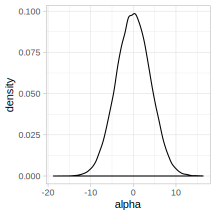
\includegraphics[width=0.45\linewidth]{bookdown_files/figure-latex/logoddspriorsf-1} 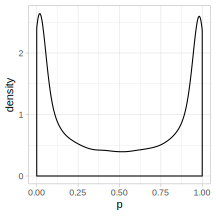
\includegraphics[width=0.45\linewidth]{bookdown_files/figure-latex/logoddspriorsf-2} \caption{Prior for \(\alpha \sim Normal(0, 4)\) in log-odds and in probability space.}\label{fig:logoddspriorsf}
\end{figure}

Figure \ref{fig:logoddspriorsf} shows that our prior assigns more probability mass to extreme probabilities of recall than to intermediate values. Clearly, this is not what we intended.

We could try several values for standard deviation of the prior, until we find a prior that make sense for us. Reducing the standard deviation to 1.5 seems to make sense as shown in Figure \ref{fig:logoddspriorsf2}.

\begin{equation}
\alpha \sim Normal(0, 1.5) \\
\end{equation}



\begin{figure}
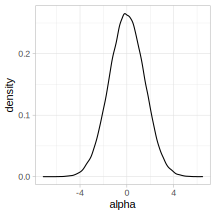
\includegraphics[width=0.45\linewidth]{bookdown_files/figure-latex/logoddspriorsf2-1} 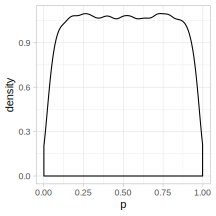
\includegraphics[width=0.45\linewidth]{bookdown_files/figure-latex/logoddspriorsf2-2} \caption{Prior for \(\alpha \sim Normal(0, 4)\) in log-odds and in probability space.}\label{fig:logoddspriorsf2}
\end{figure}

We need to decide now on the prior for the effect in log-odds of increasing the set size, \(\beta\). We are going to choose a normal distribution centered on zero, reflecting our lack of any commitment regarding the direction of the effect. Let's get some intuitions regarding different possible standard deviations for this prior, by testing the following distributions as priors:

\begin{enumerate}
\def\labelenumi{(\alph{enumi})}
\tightlist
\item
  \(\beta \sim Normal(0, 1)\)
\item
  \(\beta \sim Normal(0, .5)\)
\item
  \(\beta \sim Normal(0, .1)\)
\item
  \(\beta \sim Normal(0, .01)\)
\item
  \(\beta \sim Normal(0, .001)\)
\end{enumerate}

The following function is an edited version of the earlier \texttt{normal\_predictive\_distribution\_fast} from section \ref{sec:ppd}; it has been edited to make it compatible with logistic regression and dependent on set size:

\begin{Shaded}
\begin{Highlighting}[]
\NormalTok{logistic_model_pred <-}\StringTok{ }\ControlFlowTok{function}\NormalTok{(alpha_samples,}
\NormalTok{                                beta_samples,}
\NormalTok{                                set_size,}
\NormalTok{                                 N_obs) \{}
    \KeywordTok{map2_dfr}\NormalTok{(alpha_samples, beta_samples,}
             \ControlFlowTok{function}\NormalTok{(alpha, beta) \{}
                 \KeywordTok{tibble}\NormalTok{(}
                     \DataTypeTok{set_size =}\NormalTok{ set_size,}
                     \CommentTok{# we center size:}
                     \DataTypeTok{c_set_size =}\NormalTok{ set_size }\OperatorTok{-}\StringTok{ }\KeywordTok{mean}\NormalTok{(set_size),}
                     \CommentTok{# change the likelihood: }
                     \CommentTok{# Notice the use of a link function for alpha and beta}
                     \DataTypeTok{theta =} \KeywordTok{plogis}\NormalTok{(alpha }\OperatorTok{+}\StringTok{ }\NormalTok{c_set_size }\OperatorTok{*}\StringTok{ }\NormalTok{beta),}
                     \CommentTok{# There is no bernoulli in R, but we can just use}
                     \CommentTok{# binomial when the total number of trials is 1}
                     \DataTypeTok{correct_pred =} \KeywordTok{rbinom}\NormalTok{(N_obs, }\DataTypeTok{size =} \DecValTok{1}\NormalTok{, }\DataTypeTok{prob =}\NormalTok{ theta)}
\NormalTok{                 )}
\NormalTok{             \}, }\DataTypeTok{.id =} \StringTok{"iter"}\NormalTok{) }\OperatorTok
\StringTok{    }\CommentTok{# .id is always a string and needs to be converted to a number}
\StringTok{        }\KeywordTok{mutate}\NormalTok{(}\DataTypeTok{iter =} \KeywordTok{as.numeric}\NormalTok{(iter))}
\NormalTok{\}}
\end{Highlighting}
\end{Shaded}

Let's assume 800 observations with 200 observation of each set size:

\begin{Shaded}
\begin{Highlighting}[]
\NormalTok{N_obs <-}\StringTok{ }\DecValTok{800}
\NormalTok{set_size <-}\StringTok{ }\KeywordTok{rep}\NormalTok{(}\KeywordTok{c}\NormalTok{(}\DecValTok{2}\NormalTok{,}\DecValTok{4}\NormalTok{,}\DecValTok{6}\NormalTok{,}\DecValTok{8}\NormalTok{),}\DecValTok{200}\NormalTok{)}
\end{Highlighting}
\end{Shaded}

We iterate over the four possible standard deviations of \(\beta\):

\begin{Shaded}
\begin{Highlighting}[]
\NormalTok{alpha_samples <-}\StringTok{ }\KeywordTok{rnorm}\NormalTok{(}\DecValTok{1000}\NormalTok{, }\DecValTok{0}\NormalTok{, }\FloatTok{1.5}\NormalTok{)}
\NormalTok{sds_beta <-}\StringTok{ }\KeywordTok{c}\NormalTok{(}\DecValTok{1}\NormalTok{, }\FloatTok{0.5}\NormalTok{, }\FloatTok{0.1}\NormalTok{,}\FloatTok{0.01}\NormalTok{, }\FloatTok{0.001}\NormalTok{) }
\NormalTok{prior_pred <-}\StringTok{ }\KeywordTok{map_dfr}\NormalTok{(sds_beta, }\ControlFlowTok{function}\NormalTok{(sd) \{}
\NormalTok{    beta_samples <-}\StringTok{ }\KeywordTok{rnorm}\NormalTok{(}\DecValTok{1000}\NormalTok{, }\DecValTok{0}\NormalTok{, sd)}
    \KeywordTok{logistic_model_pred}\NormalTok{(}\DataTypeTok{alpha_samples =}\NormalTok{ alpha_samples,}
                        \DataTypeTok{beta_samples =}\NormalTok{ beta_samples,}
                        \DataTypeTok{set_size =}\NormalTok{ set_size,}
                        \DataTypeTok{N_obs =}\NormalTok{ N_obs}
\NormalTok{                        ) }\OperatorTok
\StringTok{        }\KeywordTok{mutate}\NormalTok{(}\DataTypeTok{prior_beta_sd =}\NormalTok{ sd)}
\NormalTok{\})}
\end{Highlighting}
\end{Shaded}

And we calculate the accuracy for each one of the priors we want to examine, for each iteration, and for each set size.

\begin{Shaded}
\begin{Highlighting}[]
\NormalTok{mean_accuracy <-}
\StringTok{     }\NormalTok{prior_pred }\OperatorTok
\StringTok{     }\KeywordTok{group_by}\NormalTok{(prior_beta_sd, iter, set_size) }\OperatorTok
\StringTok{     }\KeywordTok{summarize}\NormalTok{(}\DataTypeTok{accuracy =} \KeywordTok{mean}\NormalTok{(correct_pred)) }\OperatorTok
\StringTok{     }\KeywordTok{mutate}\NormalTok{(}\DataTypeTok{prior =} \KeywordTok{paste0}\NormalTok{(}\StringTok{"Normal(0, "}\NormalTok{,prior_beta_sd,}\StringTok{")"}\NormalTok{))}
\end{Highlighting}
\end{Shaded}

We plot it in Figure \ref{fig:priors4beta}, and as expected the priors are centered at zero. We see that the distribution of possible accuracies for the prior that has a standard deviation of one is problematic: There is too much probability mass concentrated near zero and one for set sizes of 2 and 8.



\begin{Shaded}
\begin{Highlighting}[]
\NormalTok{mean_accuracy }\OperatorTok
\StringTok{    }\KeywordTok{ggplot}\NormalTok{(}\KeywordTok{aes}\NormalTok{(accuracy)) }\OperatorTok{+}
\StringTok{    }\KeywordTok{geom_histogram}\NormalTok{() }\OperatorTok{+}
\StringTok{    }\KeywordTok{facet_grid}\NormalTok{(set_size}\OperatorTok{~}\NormalTok{prior)}
\end{Highlighting}
\end{Shaded}

\begin{figure}
\centering
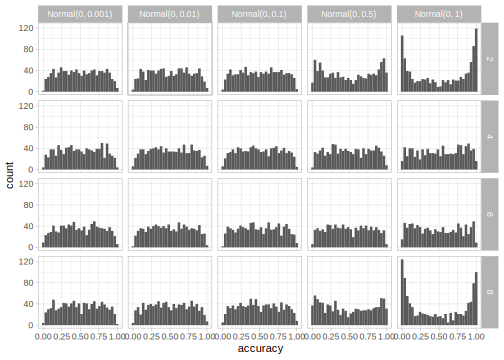
\includegraphics{bookdown_files/figure-latex/priors4beta-1.pdf}
\caption{\label{fig:priors4beta}Prior predictive distribution of mean accuracy of the model defined in \ref{sec:logistic}, for different set sizes and different priors for \(\beta\).}
\end{figure}

It's hard to tell the differences between the other priors, and it might be more useful to look at the predicted differences in accuracy between set sizes. We calculate them as follows:

\begin{Shaded}
\begin{Highlighting}[]
\NormalTok{diff_accuracy <-}\StringTok{ }\NormalTok{mean_accuracy }\OperatorTok
\StringTok{    }\KeywordTok{arrange}\NormalTok{(set_size) }\OperatorTok
\StringTok{    }\KeywordTok{group_by}\NormalTok{(iter, prior_beta_sd) }\OperatorTok
\StringTok{    }\KeywordTok{mutate}\NormalTok{(}\DataTypeTok{diffaccuracy =}\NormalTok{ accuracy }\OperatorTok{-}\StringTok{ }\KeywordTok{lag}\NormalTok{(accuracy) ) }\OperatorTok
\StringTok{    }\KeywordTok{mutate}\NormalTok{(}\DataTypeTok{diffsize =} \KeywordTok{paste}\NormalTok{(set_size,}\StringTok{"-"}\NormalTok{,  }\KeywordTok{lag}\NormalTok{(set_size))) }\OperatorTok
\StringTok{    }\KeywordTok{filter}\NormalTok{(set_size }\OperatorTok{>}\DecValTok{2}\NormalTok{)}
\end{Highlighting}
\end{Shaded}

We plot them in Figure \ref{fig:priors4beta2}. If we are not sure whether the increase of set size could produce something between a null effect and a relatively large effect, we can choose the prior with a standard deviation of \(0.5\).



\begin{Shaded}
\begin{Highlighting}[]
\NormalTok{diff_accuracy }\OperatorTok
\StringTok{    }\KeywordTok{ggplot}\NormalTok{(}\KeywordTok{aes}\NormalTok{(diffaccuracy)) }\OperatorTok{+}
\StringTok{    }\KeywordTok{geom_histogram}\NormalTok{() }\OperatorTok{+}
\StringTok{    }\KeywordTok{facet_grid}\NormalTok{(diffsize}\OperatorTok{~}\NormalTok{prior)}
\end{Highlighting}
\end{Shaded}

\begin{figure}
\centering
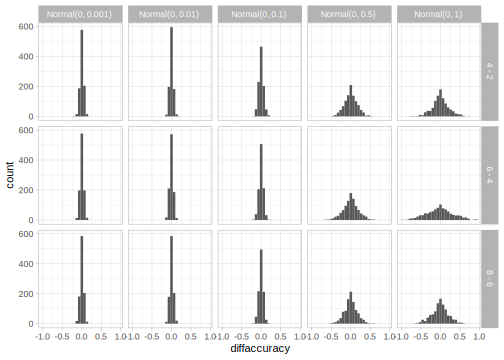
\includegraphics{bookdown_files/figure-latex/priors4beta2-1.pdf}
\caption{\label{fig:priors4beta2}Prior predictive distribution of differences in mean accuracy between set sizes of the model defined in \ref{sec:logistic} for different priors for \(\beta\).}
\end{figure}

We settle one the following priors:

\begin{equation}
\begin{aligned}
\alpha &\sim Normal(0, 1.5) \\
\beta &\sim Normal(0, 0.5) 
\end{aligned}
\end{equation}

\hypertarget{the-brms-model-2}{%
\subsection{\texorpdfstring{The \texttt{brms} model}{The brms model}}\label{the-brms-model-2}}

Having decided on the likelihood, the link function, and the priors, the model can now be fit using \texttt{brms}. Notice that we need to specify that the family is \texttt{bernoulli()}, and the link is \texttt{logit}.

\begin{Shaded}
\begin{Highlighting}[]
\NormalTok{df_recall_data <-}\StringTok{ }\KeywordTok{read_table2}\NormalTok{(}\StringTok{"./data/PairsRSS1_all.dat"}\NormalTok{,}
                              \DataTypeTok{col_names =} \KeywordTok{c}\NormalTok{(}\StringTok{"subject"}\NormalTok{, }\StringTok{"session"}\NormalTok{, }\StringTok{"block"}\NormalTok{,}
                                            \StringTok{"trial"}\NormalTok{, }\StringTok{"set_size"}\NormalTok{,}
                                            \StringTok{"response_size_list"}\NormalTok{,}
                                            \StringTok{"response_size_new_words"}\NormalTok{,}
                                            \StringTok{"tested"}\NormalTok{, }\StringTok{"response"}\NormalTok{,}
                                            \StringTok{"response_category"}\NormalTok{, }\StringTok{"rt"}\NormalTok{)) }\OperatorTok
\StringTok{    }\CommentTok{# ignore the type of incorrect responses (the focus of the paper)}
\StringTok{    }\KeywordTok{mutate}\NormalTok{(}\DataTypeTok{correct =} \KeywordTok{if_else}\NormalTok{(response_category }\OperatorTok{==}\DecValTok{1}\NormalTok{, }\DecValTok{1}\NormalTok{, }\DecValTok{0}\NormalTok{)) }\OperatorTok
\StringTok{    }\CommentTok{# use only the data from the free recall task:}
\StringTok{    }\CommentTok{# (when there was no list of possible responses)}
\StringTok{    }\KeywordTok{filter}\NormalTok{(response_size_list }\OperatorTok{+}\StringTok{ }\NormalTok{response_size_new_words }\OperatorTok{==}\StringTok{ }\DecValTok{0}\NormalTok{) }\OperatorTok
\StringTok{    }\CommentTok{# select one subject}
\StringTok{    }\KeywordTok{filter}\NormalTok{(subject }\OperatorTok{==}\StringTok{ }\DecValTok{10}\NormalTok{) }\OperatorTok
\StringTok{    }\KeywordTok{mutate}\NormalTok{(}\DataTypeTok{c_set_size =}\NormalTok{ set_size }\OperatorTok{-}\StringTok{ }\KeywordTok{mean}\NormalTok{(set_size))}
\CommentTok{# ignore the warning from read_table}

\CommentTok{# Set sizes in the dataset:}
\NormalTok{df_recall_data}\OperatorTok{$}\NormalTok{set_size }\OperatorTok
\StringTok{    }\NormalTok{unique}
\end{Highlighting}
\end{Shaded}

\begin{verbatim}
## [1] 4 8 2 6
\end{verbatim}

\begin{Shaded}
\begin{Highlighting}[]
\CommentTok{# Trials by set size}
\NormalTok{df_recall_data }\OperatorTok
\StringTok{    }\KeywordTok{group_by}\NormalTok{(set_size) }\OperatorTok
\StringTok{    }\KeywordTok{count}\NormalTok{()}
\end{Highlighting}
\end{Shaded}

\begin{verbatim}
## # A tibble: 4 x 2
## # Groups:   set_size [4]
##   set_size     n
##      <dbl> <int>
## 1        2    23
## 2        4    23
## 3        6    23
## 4        8    23
\end{verbatim}

\begin{Shaded}
\begin{Highlighting}[]
\NormalTok{fit_recall <-}\StringTok{ }\KeywordTok{brm}\NormalTok{(correct }\OperatorTok{~}\StringTok{ }\DecValTok{1} \OperatorTok{+}\StringTok{ }\NormalTok{c_set_size,}
  \DataTypeTok{data =}\NormalTok{ df_recall_data,}
  \DataTypeTok{family =} \KeywordTok{bernoulli}\NormalTok{(}\DataTypeTok{link =}\NormalTok{ logit),}
  \DataTypeTok{prior =} \KeywordTok{c}\NormalTok{(}
    \KeywordTok{prior}\NormalTok{(}\KeywordTok{normal}\NormalTok{(}\DecValTok{0}\NormalTok{, }\FloatTok{1.5}\NormalTok{), }\DataTypeTok{class =}\NormalTok{ Intercept),}
    \KeywordTok{prior}\NormalTok{(}\KeywordTok{normal}\NormalTok{(}\DecValTok{0}\NormalTok{, }\FloatTok{.5}\NormalTok{), }\DataTypeTok{class =}\NormalTok{ b, }\DataTypeTok{coef =}\NormalTok{ c_set_size)}
\NormalTok{  )}
\NormalTok{)}
\end{Highlighting}
\end{Shaded}

Next, look at the summary of the posteriors of each of the parameters. Keep in mind that the parameters are in log-odds space:

\begin{Shaded}
\begin{Highlighting}[]
\KeywordTok{posterior_summary}\NormalTok{(fit_recall)[}\DecValTok{1}\OperatorTok{:}\DecValTok{2}\NormalTok{,}\KeywordTok{c}\NormalTok{(}\DecValTok{1}\NormalTok{,}\DecValTok{3}\NormalTok{,}\DecValTok{4}\NormalTok{)]}
\end{Highlighting}
\end{Shaded}

\begin{verbatim}
##              Estimate  Q2.5 Q97.5
## b_Intercept      2.45  1.70  3.40
## b_c_set_size    -0.61 -0.99 -0.29
\end{verbatim}

Plot the posteriors as well:

\begin{Shaded}
\begin{Highlighting}[]
\KeywordTok{plot}\NormalTok{(fit_recall)}
\end{Highlighting}
\end{Shaded}

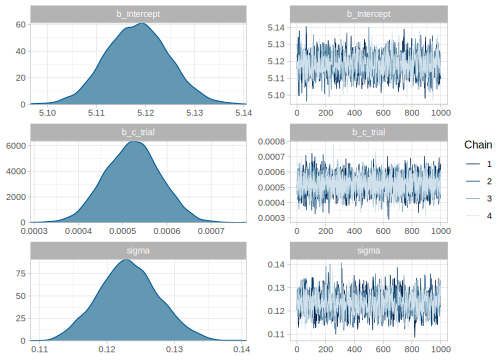
\includegraphics{bookdown_files/figure-latex/unnamed-chunk-112-1.pdf}

Next, we turn to the question of what we can report as our results, and what we can conclude from the data.

\hypertarget{how-to-communicate-the-results-2}{%
\subsection{How to communicate the results?}\label{how-to-communicate-the-results-2}}

We are here in situation analogous as before with the log-normal model. If we want to talk about the effect estimated by the model in log-odds space, we summarize the posterior of \(\beta\) in the following way: \(\hat\beta = -0.61\), 95\% CrI = \([ -0.99 , -0.29 ]\).

However, the effect might be easier to understand in proportions rather than in log-odds. Let's look at the average accuracy for the task first:

\begin{Shaded}
\begin{Highlighting}[]
\NormalTok{alpha_samples<-}\StringTok{ }\KeywordTok{posterior_samples}\NormalTok{(fit_recall)}\OperatorTok{$}\NormalTok{b_Intercept}
\NormalTok{av_accuracy <-}\StringTok{ }\KeywordTok{plogis}\NormalTok{(alpha_samples)}
\KeywordTok{c}\NormalTok{(}\DataTypeTok{mean =} \KeywordTok{mean}\NormalTok{(av_accuracy), }\KeywordTok{quantile}\NormalTok{(av_accuracy, }\KeywordTok{c}\NormalTok{(.}\DecValTok{025}\NormalTok{,.}\DecValTok{975}\NormalTok{)))}
\end{Highlighting}
\end{Shaded}

\begin{verbatim}
## mean 2.5%  98% 
## 0.92 0.85 0.97
\end{verbatim}

As before, to transform the effect of our manipulation to an easier to interpret scale (i.e., proportion), we need to take into account that the scale is not linear, and that the effect of increasing the set size depends on the average accuracy, and the set size that we start from.

We can do the following calculation, similar to what we did for the trial effects experiment, to find out the decrease in accuracy in proportions or probability scale:

\begin{Shaded}
\begin{Highlighting}[]
\NormalTok{beta_samples<-}\StringTok{ }\KeywordTok{posterior_samples}\NormalTok{(fit_recall)}\OperatorTok{$}\NormalTok{b_c_set_size}
\NormalTok{effect_middle <-}\StringTok{ }\KeywordTok{plogis}\NormalTok{(alpha_samples) }\OperatorTok{-}\StringTok{ }\KeywordTok{plogis}\NormalTok{(alpha_samples }\OperatorTok{-}\StringTok{ }\NormalTok{beta_samples)}
\KeywordTok{c}\NormalTok{(}\DataTypeTok{mean =} \KeywordTok{mean}\NormalTok{(effect_middle), }\KeywordTok{quantile}\NormalTok{(effect_middle, }\KeywordTok{c}\NormalTok{(.}\DecValTok{025}\NormalTok{,.}\DecValTok{975}\NormalTok{)))}
\end{Highlighting}
\end{Shaded}

\begin{verbatim}
##   mean   2.5%    98% 
## -0.034 -0.055 -0.017
\end{verbatim}

Notice the interpretation here, if we increase the set size from the average set size minus one to the average set size, we get a reduction in the accuracy of recall of \(-0.03\), 95\% CrI = \([ -0.06 , -0.02 ]\). Recall that the average set size, 5, was not presented to the subject! We could also look at the decrease in accuracy from a set size of 2 to 4:

\begin{Shaded}
\begin{Highlighting}[]
\NormalTok{effect_4m2 <-}\StringTok{ }\KeywordTok{plogis}\NormalTok{(alpha_samples}\OperatorTok{+}\StringTok{  }\NormalTok{(}\DecValTok{4} \OperatorTok{-}\StringTok{ }\KeywordTok{mean}\NormalTok{(df_recall_data}\OperatorTok{$}\NormalTok{set_size)) }\OperatorTok{*}\StringTok{ }\NormalTok{beta_samples) }\OperatorTok{-}
\StringTok{    }\KeywordTok{plogis}\NormalTok{(alpha_samples}\OperatorTok{+}\StringTok{  }\NormalTok{(}\DecValTok{2} \OperatorTok{-}\StringTok{ }\KeywordTok{mean}\NormalTok{(df_recall_data}\OperatorTok{$}\NormalTok{set_size)) }\OperatorTok{*}\StringTok{ }\NormalTok{beta_samples)}
\KeywordTok{c}\NormalTok{(}\DataTypeTok{mean =} \KeywordTok{mean}\NormalTok{(effect_4m2), }\KeywordTok{quantile}\NormalTok{(effect_4m2, }\KeywordTok{c}\NormalTok{(.}\DecValTok{025}\NormalTok{,.}\DecValTok{975}\NormalTok{)))}
\end{Highlighting}
\end{Shaded}

\begin{verbatim}
##   mean   2.5%    98% 
## -0.032 -0.057 -0.011
\end{verbatim}

We see that increasing the set size does have a detrimental effect in recall, as we suspected.

\hypertarget{descriptive-adequacy}{%
\subsection{Descriptive adequacy}\label{descriptive-adequacy}}

One potentially useful aspect of posterior distributions is that we could also make predictions for other conditions not presented in the actual experiment, such as set sizes that weren't tested. We could then verify if our model was right with another experiment. To make predictions for other set sizes, we extend our dataset adding rows with set sizes of 3, 5, and 7. To be consistent with the data of the other set sizes in the experiment, we add 23 trials of each new set size (this is the number of trial by set sizes in the dataset). Something important to notice is that \textbf{we need to center our predictor based on the original mean set size}. This is because we want to maintain our interpretation of the intercept. We extend the data as follows, and we summarize the data and plot it in Figure \ref{fig:postpredsum2}.

\begin{Shaded}
\begin{Highlighting}[]
\NormalTok{df_recall_data_ext <-}\StringTok{ }\NormalTok{df_recall_data }\OperatorTok
\StringTok{    }\KeywordTok{bind_rows}\NormalTok{(}\KeywordTok{tibble}\NormalTok{(}\DataTypeTok{set_size =} \KeywordTok{rep}\NormalTok{(}\KeywordTok{c}\NormalTok{(}\DecValTok{3}\NormalTok{,}\DecValTok{5}\NormalTok{,}\DecValTok{7}\NormalTok{),}\DecValTok{23}\NormalTok{),}
                     \DataTypeTok{c_set_size =}\NormalTok{ set_size }\OperatorTok{-}\StringTok{ }\KeywordTok{mean}\NormalTok{(df_recall_data}\OperatorTok{$}\NormalTok{set_size)))}
\NormalTok{df_recall_pred_ext <-}\StringTok{ }\KeywordTok{posterior_predict}\NormalTok{(fit_recall,}
                                 \DataTypeTok{newdata =}\NormalTok{ df_recall_data_ext,}
                                 \DataTypeTok{nsamples =} \DecValTok{1000}\NormalTok{) }\OperatorTok
\StringTok{    }\KeywordTok{array_branch}\NormalTok{(}\DataTypeTok{margin =} \DecValTok{1}\NormalTok{) }\OperatorTok
\StringTok{    }\KeywordTok{map_dfr}\NormalTok{( }\ControlFlowTok{function}\NormalTok{(yrep_iter) \{}
\NormalTok{        df_recall_data_ext }\OperatorTok
\StringTok{            }\KeywordTok{mutate}\NormalTok{(}\DataTypeTok{correct =}\NormalTok{ yrep_iter)}
\NormalTok{    \}, }\DataTypeTok{.id =} \StringTok{"iter"}\NormalTok{) }\OperatorTok
\StringTok{    }\KeywordTok{mutate}\NormalTok{(}\DataTypeTok{iter =} \KeywordTok{as.numeric}\NormalTok{(iter))}
\end{Highlighting}
\end{Shaded}



\begin{Shaded}
\begin{Highlighting}[]
\NormalTok{df_recall_pred_ext_summary <-}\StringTok{ }\NormalTok{df_recall_pred_ext }\OperatorTok
\StringTok{    }\KeywordTok{group_by}\NormalTok{(iter, set_size) }\OperatorTok
\StringTok{    }\KeywordTok{summarize}\NormalTok{(}\DataTypeTok{accuracy =} \KeywordTok{mean}\NormalTok{(correct))}
\CommentTok{# observed means:}
\NormalTok{df_recall_summary<-}\StringTok{ }\NormalTok{df_recall_data }\OperatorTok
\StringTok{    }\KeywordTok{group_by}\NormalTok{(set_size) }\OperatorTok
\StringTok{    }\KeywordTok{summarize}\NormalTok{(}\DataTypeTok{accuracy =} \KeywordTok{mean}\NormalTok{(correct))}
\KeywordTok{ggplot}\NormalTok{(df_recall_pred_ext_summary, }\KeywordTok{aes}\NormalTok{(accuracy)) }\OperatorTok{+}
\StringTok{    }\KeywordTok{geom_histogram}\NormalTok{(}\DataTypeTok{alpha=}\NormalTok{.}\DecValTok{5}\NormalTok{)}\OperatorTok{+}
\StringTok{    }\KeywordTok{geom_vline}\NormalTok{(}\KeywordTok{aes}\NormalTok{(}\DataTypeTok{xintercept=}\NormalTok{ accuracy),}\DataTypeTok{data=}\NormalTok{ df_recall_summary)}\OperatorTok{+}
\StringTok{    }\KeywordTok{facet_grid}\NormalTok{(set_size }\OperatorTok{~}\StringTok{ }\NormalTok{.)}
\end{Highlighting}
\end{Shaded}

\begin{figure}
\centering
\includegraphics{bookdown_files/figure-latex/postpredsum2-1.pdf}
\caption{\label{fig:postpredsum2}Distribution of posterior predicted mean accuracies in gray for tested set sizes (2, 4, 6, and 8) and untested ones (3, 5, and 7), and observed mean accuracy in black lines by tested set sizes.}
\end{figure}

\hypertarget{summary-1}{%
\section{Summary}\label{summary-1}}

\hypertarget{further-reading-3}{%
\section{Further reading}\label{further-reading-3}}

\hypertarget{exercises-3}{%
\section{Exercises}\label{exercises-3}}

\begin{enumerate}
\def\labelenumi{\arabic{enumi}.}
\tightlist
\item
  For the lognormal model (section \ref{sec:trial}:

  \begin{enumerate}
  \def\labelenumii{\arabic{enumii}.}
  \tightlist
  \item
    Estimate the slowdown in milliseconds for the last time the subject pressed the space bar in the experiment. In addition, predict the slowdown if the experiment would have had 500 observations. Does it work? What does it tell us about our covariate?
  \end{enumerate}
\end{enumerate}

\hypertarget{appendix-1}{%
\section{Appendix}\label{appendix-1}}

\hypertarget{sec:preprocessingpupil}{%
\subsection{Preparation of the pupil size data (section \ref{sec:pupil})}\label{sec:preprocessingpupil}}

We prepared the data for the linear model of section \ref{sec:pupil} with a dataset from \citet{wahnPupilSizesScale2016} downloaded from (\url{https://osf.io/z43dz/}). The following code creates the pilot data and the averages by trial.

\begin{Shaded}
\begin{Highlighting}[]
\NormalTok{df_pupil_full_control <-}\StringTok{ }\KeywordTok{read_csv}\NormalTok{(}\StringTok{"./data/PLOS_raw_pupildata_controlexperiment.csv"}\NormalTok{) }\OperatorTok
\StringTok{    }\KeywordTok{rename}\NormalTok{(}\DataTypeTok{p_size =}\NormalTok{ Pupilsize, }\DataTypeTok{load =}\NormalTok{ Attentionalload, }\DataTypeTok{trial =}\NormalTok{ Trial, }\DataTypeTok{time =}\NormalTok{ Time)}
\CommentTok{# "Pilot" data}
\NormalTok{df_pupil_pilot <-}\StringTok{ }\NormalTok{df_pupil_full_control }\OperatorTok
\StringTok{    }\KeywordTok{filter}\NormalTok{(Subnum}\OperatorTok{==}\DecValTok{701}\NormalTok{, load }\OperatorTok{==}\DecValTok{0}\NormalTok{,time }\OperatorTok{<}\DecValTok{100}\NormalTok{, trial }\OperatorTok{==}\DecValTok{5}\NormalTok{) }\OperatorTok
\StringTok{    }\KeywordTok{select}\NormalTok{(time, p_size, load)}
\KeywordTok{write_csv}\NormalTok{(df_pupil_pilot, }\StringTok{"./data/pupil_pilot.csv"}\NormalTok{)}
\CommentTok{# Averaged by trial data}
\NormalTok{df_pupil <-}\StringTok{ }\NormalTok{df_pupil_full_control }\OperatorTok
\StringTok{    }\KeywordTok{filter}\NormalTok{(Subnum}\OperatorTok{==}\DecValTok{701}\NormalTok{, time }\OperatorTok{>}\StringTok{ }\DecValTok{100}\NormalTok{) }\OperatorTok
\StringTok{    }\KeywordTok{group_by}\NormalTok{(trial, load) }\OperatorTok
\StringTok{    }\KeywordTok{summarize}\NormalTok{(}\DataTypeTok{p_size =} \KeywordTok{mean}\NormalTok{(p_size, }\DataTypeTok{na.rm=} \OtherTok{TRUE}\NormalTok{))}
\KeywordTok{write_csv}\NormalTok{(df_pupil, }\StringTok{"./data/pupil.csv"}\NormalTok{)}
\end{Highlighting}
\end{Shaded}

\hypertarget{bayesian-hierarchical-models}{%
\chapter{Bayesian hierarchical models}\label{bayesian-hierarchical-models}}

Usually, experimental data in cognitive science contain ``clusters''. These are natural groups that contain observations that are more similar within the clusters than between them.
The most common examples of clusters in experimental designs are participants and items. These clusters arise because we have multiple (repeated) observations for each participant, and for each item. If we want to incorporate this structure in our analysis, we need to use a hierarchical model (also called multi-level and mixed models).

The notion of exchangeability is important to understand in hierarchical models. Suppose we assign a numerical index to each of the levels of a cluster (e.g., to each participant). When the levels are exchangeable, we can reassign the indices arbitrarily and lose no information. In hierarchical models, we treat the clusters as exchangeable, and observations within each cluster as also exchangeable. In practice, we include predictors at the level of the observations, those are the predictors that correspond to the experimental manipulations (e.g., attentional load, trial number, Cloze probability, etc.); and maybe also at the cluster level, these are predictors that indicate characteristics of the cluster (e.g., working memory capacity score of each participant). Then the conditional distributions given these explanatory variables would be exchangeable, that is, our predictors incorporate all the information that is not exchangeable, and when we factor the predictors out, the observations or clusters are exchangeable. This is the reason why while the item number is an appropriate cluster (the indexes are exchangeable), trial number is not. See Chapter 5 of \citet{Gelman14} for a more technical treatment of exchangeability.

\BeginKnitrBlock{rmdnote}
to-do: make this better
\EndKnitrBlock{rmdnote}

\hypertarget{a-hierarchical-normal-model-the-n400-effect}{%
\section{A hierarchical normal model: The N400 effect}\label{a-hierarchical-normal-model-the-n400-effect}}

Event-related potentials (ERPs) allow scientists to observe electrophysiological responses in the brain measured by means of electroencephalography (EEG) that are time-locked to a specific event (i.e., the presentation of the stimuli). A very robust ERP effect in the study of language is the so-called N400. It has been shown that words with low predictability are accompanied by an \emph{N400 effect} in comparison with high-predictable words, this is a relative negativity that peaks around 300-500 after word onset over central parietal scalp sites \citetext{\citealp[first noticed in][]{kutasReadingSenselessSentences1980}; \citealp[for semantic anomalies and in][ for low predictable word]{kutasBrainPotentialsReading1984}; \citealp[for a review:][]{kutasThirtyYearsCounting2011}}.

\BeginKnitrBlock{rmdnote}
to-do: N400 plot here
\EndKnitrBlock{rmdnote}

In 1, for example, the continuation \emph{`paint'} has higher predictability than the continuation \emph{`dog'}, and thus we would expect a more negative signal, that is, an N400 effect, in \emph{`dog'} in (b) in comparison with \emph{`paint'} in (a). It is often the case that predictability is measured with a Cloze task (see section \ref{sec:binomialcloze}).

\begin{enumerate}
\def\labelenumi{\arabic{enumi}.}
\tightlist
\item
  Example from \citet{kutasBrainPotentialsReading1984}

  \begin{enumerate}
  \def\labelenumii{\alph{enumii}.}
  \tightlist
  \item
    Don't touch the wet paint.
  \item
    Don't touch the wet dog.
  \end{enumerate}
\end{enumerate}

The EEG data are typically recorded in tens of electrodes every couple of milliseconds, but for our purposes (i.e., for learning about Bayesian hierarchical models), we can safely ignore the complexity of the data. A common way to simplify the high-dimensional EEG data when we are dealing with the N400 is to focus on the average amplitude of the EEG signal at its typical spatio-temporal window of the N400 \citep[see for example][]{frankERPResponseAmount2015}.

For this example, we are going to focus on the N400 effect for critical nouns from a subset of the data of \citet{nieuwlandLargescaleReplicationStudy2018}. \citet{nieuwlandLargescaleReplicationStudy2018} presented a replication attempt of an original experiment of \citet{delongProbabilisticWordPreactivation2005} with sentences like (2)

\begin{enumerate}
\def\labelenumi{\arabic{enumi}.}
\setcounter{enumi}{1}
\tightlist
\item
  Example from \citet{delongProbabilisticWordPreactivation2005}

  \begin{enumerate}
  \def\labelenumii{\alph{enumii}.}
  \tightlist
  \item
    The day was breezy so the boy went outside to fly a kite.
  \item
    The day was breezy so the boy went outside to fly an airplane.
  \end{enumerate}
\end{enumerate}

We'll ignore the goal of original experiment \citep{delongProbabilisticWordPreactivation2005}, and its replication \citep{nieuwlandLargescaleReplicationStudy2018}. We are going to focus on the N400 at the final nouns in the experimental stimuli. In example (2), for example, the final noun \emph{`kite'} has higher predictability than \emph{`airplane'}, and thus we would expect a more negative signal in \emph{`airplane'} in (b) in comparison with \emph{`kite'} in (a).

To speed-up computation, we'll restrict the dataset to the participants from the Edinburgh lab; the entire dataset can be found in \url{https://osf.io/q7dsk/}.

\begin{Shaded}
\begin{Highlighting}[]
\NormalTok{df_eeg_data <-}\StringTok{ }\KeywordTok{read_tsv}\NormalTok{(}\StringTok{"data/public_noun_data.txt"}\NormalTok{) }\OperatorTok
\StringTok{    }\KeywordTok{filter}\NormalTok{(lab}\OperatorTok{==}\StringTok{"edin"}\NormalTok{)}
\NormalTok{df_eeg_data}
\end{Highlighting}
\end{Shaded}

\begin{verbatim}
## # A tibble: 2,827 x 6
##   subject segment cloze lab    item  n400
##   <chr>     <dbl> <dbl> <chr> <dbl> <dbl>
## 1 edin1         1     0 edin    101  7.08
## 2 edin1         2     3 edin    102 -0.68
## 3 edin1         3   100 edin    103  1.39
## 4 edin1         4    93 edin    104 22.8 
## 5 edin1         5     0 edin    105  1.61
## # ... with 2,822 more rows
\end{verbatim}

\begin{Shaded}
\begin{Highlighting}[]
\CommentTok{# Number of subjects}
\NormalTok{df_eeg_data }\OperatorTok
\StringTok{    }\KeywordTok{distinct}\NormalTok{(subject) }\OperatorTok
\StringTok{    }\KeywordTok{count}\NormalTok{()}
\end{Highlighting}
\end{Shaded}

\begin{verbatim}
## # A tibble: 1 x 1
##       n
##   <int>
## 1    37
\end{verbatim}

\begin{Shaded}
\begin{Highlighting}[]
\CommentTok{## choose only the relevant columns:}
\NormalTok{df_eeg_data<-df_eeg_data[,}\KeywordTok{c}\NormalTok{(}\DecValTok{1}\NormalTok{,}\DecValTok{3}\NormalTok{,}\DecValTok{5}\NormalTok{,}\DecValTok{6}\NormalTok{)]}
\CommentTok{## strip edin prefix on subject names:}
\NormalTok{df_eeg_data}\OperatorTok{$}\NormalTok{subject<-stringr}\OperatorTok{::}\KeywordTok{str_replace}\NormalTok{(df_eeg_data}\OperatorTok{$}\NormalTok{subject,}\StringTok{"edin"}\NormalTok{,}\StringTok{""}\NormalTok{)}
\CommentTok{## save unique subject ids:}
\NormalTok{subj_levels<-}\KeywordTok{sort}\NormalTok{(}\KeywordTok{unique}\NormalTok{(}\KeywordTok{as.numeric}\NormalTok{(}\KeywordTok{as.character}\NormalTok{(df_eeg_data}\OperatorTok{$}\NormalTok{subject))))}
\NormalTok{df_eeg_data}\OperatorTok{$}\NormalTok{subject<-}\KeywordTok{factor}\NormalTok{(df_eeg_data}\OperatorTok{$}\NormalTok{subject,}\DataTypeTok{levels=}\NormalTok{subj_levels)}
\end{Highlighting}
\end{Shaded}

In the data, the Cloze is in percentages, we'll transform it to proportions and center it before using it as a predictor in \texttt{c\_cloze}.

\begin{Shaded}
\begin{Highlighting}[]
\NormalTok{df_eeg_data  <-}\StringTok{ }\NormalTok{df_eeg_data }\OperatorTok
\StringTok{    }\KeywordTok{mutate}\NormalTok{(}\DataTypeTok{c_cloze=}\NormalTok{ cloze}\OperatorTok{/}\DecValTok{100} \OperatorTok{-}\StringTok{ }\KeywordTok{mean}\NormalTok{(cloze}\OperatorTok{/}\DecValTok{100}\NormalTok{) )}
\NormalTok{df_eeg_data}\OperatorTok{$}\NormalTok{c_cloze }\OperatorTok\StringTok{ }\KeywordTok{summary}\NormalTok{() }
\end{Highlighting}
\end{Shaded}

\begin{verbatim}
##    Min. 1st Qu.  Median    Mean 3rd Qu.    Max. 
##   -0.47   -0.44    0.03    0.00    0.43    0.53
\end{verbatim}

One nice aspect of using averages of EEG data is that they are roughly normally distributed. This allows us to use the Normal likelihood. Here is a histogram showing the distribution of the data:

\begin{Shaded}
\begin{Highlighting}[]
\NormalTok{df_eeg_data }\OperatorTok\StringTok{ }\KeywordTok{ggplot}\NormalTok{(}\KeywordTok{aes}\NormalTok{(n400)) }\OperatorTok{+}
\StringTok{    }\KeywordTok{geom_histogram}\NormalTok{(}\DataTypeTok{binwidth =} \DecValTok{4}\NormalTok{, }\DataTypeTok{colour=}\StringTok{"gray"}\NormalTok{, }\DataTypeTok{alpha =} \FloatTok{.5}\NormalTok{, }\KeywordTok{aes}\NormalTok{(}\DataTypeTok{y =}\NormalTok{ ..density..)) }\OperatorTok{+}
\StringTok{    }\KeywordTok{stat_function}\NormalTok{(}\DataTypeTok{fun =}\NormalTok{ dnorm, }\DataTypeTok{args =} \KeywordTok{list}\NormalTok{(}
                                                 \DataTypeTok{mean =} \KeywordTok{mean}\NormalTok{(df_eeg_data}\OperatorTok{$}\NormalTok{n400),}
                                                 \DataTypeTok{sd =} \KeywordTok{sd}\NormalTok{(df_eeg_data}\OperatorTok{$}\NormalTok{n400))) }\OperatorTok{+}
\StringTok{    }\KeywordTok{xlab}\NormalTok{(}\StringTok{"Average voltage in microvolts for the N400 spatiotemporal window"}\NormalTok{)}
\end{Highlighting}
\end{Shaded}

\begin{figure}
\centering
\includegraphics{bookdown_files/figure-latex/unnamed-chunk-122-1.pdf}
\caption{\label{fig:unnamed-chunk-122}Histogram of the N400 averages for every trial in gray; density plot of a normal distribution in black.}
\end{figure}

\hypertarget{complete-pooling-model-m_cp}{%
\subsection{\texorpdfstring{Complete-pooling model (\(M_{cp}\))}{Complete-pooling model (M\_\{cp\})}}\label{complete-pooling-model-m_cp}}

We'll start from the simplest model which is basically the linear regression we encountered in the preceding chapter.

\hypertarget{model-assumptions}{%
\subsubsection{Model assumptions}\label{model-assumptions}}

This model, call it \(M_{cp}\), makes the following assumptions.

\begin{enumerate}
\def\labelenumi{\arabic{enumi}.}
\tightlist
\item
  The EEG averages for the N400 spatiotemporal window are normally distributed.
\item
  Observations are \emph{independent}.
\item
  There is a linear relationship between cloze and the EEG signal for the trial.
\end{enumerate}

\textbf{Note that this model is incorrect for these data due to assumption 2 being violated.}

With the last assumption, we are saying that the difference in the average signal when we compare nouns with Cloze probability 0-.1, .1-.2, .2-.3, and so forth is the same. Notice that this \emph{is} an assumption, and it may not necessarily be the case in the actual data. This means that we are going to get a posterior for \(\beta\) \emph{conditional} on the assumption that the linear relationship holds. Even if it \emph{approximately} holds, we still don't know how much we deviate from this assumption. We'll come back to this issue in chapter ?? when we deal with model comparison.

We can now decide on a likelihood and priors:

\hypertarget{likelihood-and-priors-1}{%
\subsubsection{Likelihood and priors}\label{likelihood-and-priors-1}}

A normal likelihood seems reasonable for these data:

\begin{equation}
   signal_n \sim Normal( \alpha + c\_cloze_n \cdot \beta,\sigma)
  \label{eq:Mcp}
 \end{equation}

where \(n =1, \ldots, N\), and \(rt\) is the dependent variable (reaction times in milliseconds). The variable \(N\) represents the total number of data points.

As always we need to rely on our previous knowledge and domain expertise to decide on priors. We know that ERPs (signals time-locked to a stimulus) have mean amplitudes of a couple of microvolts, this is easy to see in any plot of the EEG literature. This means that we don't expect the effect of our manipulation to exceed, say, 10 \(\mu V\). As before we'll assume that effects can be negative or positive. We can quantify our prior knowledge regarding plausible values of \(\beta\) as a normal distributed centered at zero with a standard deviation of 10 \(\mu V\).

If the signal for each ERP is \emph{baselined}, that is, the mean signal of a time window before the time window of interest is subtracted to the time window of interest, then the mean signal would be relatively close to 0. Since we know the ERPs were baselined in this study, we expect that the grand mean of our signal should be relatively close to zero. Our prior for \(\alpha\) is then normally distributed centered in zero with a standard deviation of 10 \(\mu V\).

The standard deviation of our signal distribution is harder to guess. We know that EEG signals are quite noisy, and that the standard deviation must be higher than zero. Our prior for \(\sigma\) is a truncated normal distribution with location zero and scale as 50. Notice that since we truncate the distribution, the parameters location and scale do not correspond to mean and standard deviation; we can see this by drawing random samples from this distribution and calculating their mean and standard deviation:

\begin{Shaded}
\begin{Highlighting}[]
\NormalTok{samples <-}\StringTok{ }\KeywordTok{rtnorm}\NormalTok{(}\DecValTok{1000}\NormalTok{,}\DecValTok{0}\NormalTok{ ,}\DecValTok{50}\NormalTok{, }\DataTypeTok{a=}\DecValTok{0}\NormalTok{)}
\KeywordTok{c}\NormalTok{(}\DataTypeTok{mean =} \KeywordTok{mean}\NormalTok{(samples), }\KeywordTok{sd}\NormalTok{(samples))}
\end{Highlighting}
\end{Shaded}

\begin{verbatim}
## mean      
##   40   31
\end{verbatim}

So we are essentially saying that we assume a prior that we will find the true standard deviation of the signal in the following interval with 95\% probability:

\begin{Shaded}
\begin{Highlighting}[]
\KeywordTok{quantile}\NormalTok{(samples, }\KeywordTok{c}\NormalTok{(}\FloatTok{0.025}\NormalTok{,.}\DecValTok{975}\NormalTok{))}
\end{Highlighting}
\end{Shaded}

\begin{verbatim}
##  2.5%   98% 
##   1.7 111.1
\end{verbatim}

To sum up, we are going to use the following Priors:

\begin{equation}
 \begin{aligned}
 \alpha &\sim Normal(0,10)\\
 \beta  &\sim Normal(0,10)\\
 \sigma  &\sim Normal_{+}(0,50)
 \end{aligned}
 \end{equation}

A model such as \(M_{cp}\) is sometimes called a \emph{fixed-effects} model: all the parameters are fixed and do not vary from subject to subject or from item to item. A similar frequentist model would correspond to fitting a simple linear model using the \texttt{lm} function: \texttt{lm(n400\ \textasciitilde{}\ 1\ +\ cloze,\ data=df\_eeg\_data)}.

We fit this model in \texttt{brms} as follows (the default family is \texttt{gaussian()} so we can omit it). As with \texttt{lm}, by default an intercept is fitted and thus \texttt{n400\ \textasciitilde{}\ c\_cloze} is equivalent to \texttt{n400\ \textasciitilde{}\ 1\ +\ c\_cloze}:

\begin{Shaded}
\begin{Highlighting}[]
\NormalTok{fit_N400_cp <-}\StringTok{ }\KeywordTok{brm}\NormalTok{(n400 }\OperatorTok{~}\StringTok{ }\NormalTok{c_cloze,}
  \DataTypeTok{prior =} 
    \KeywordTok{c}\NormalTok{(}\KeywordTok{prior}\NormalTok{(}\KeywordTok{normal}\NormalTok{(}\DecValTok{0}\NormalTok{, }\DecValTok{10}\NormalTok{), }\DataTypeTok{class =}\NormalTok{ Intercept),}
      \KeywordTok{prior}\NormalTok{(}\KeywordTok{normal}\NormalTok{(}\DecValTok{0}\NormalTok{, }\DecValTok{10}\NormalTok{), }\DataTypeTok{class =}\NormalTok{ b, }\DataTypeTok{coef =}\NormalTok{ c_cloze),}
      \KeywordTok{prior}\NormalTok{(}\KeywordTok{normal}\NormalTok{(}\DecValTok{0}\NormalTok{, }\DecValTok{50}\NormalTok{), }\DataTypeTok{class =}\NormalTok{ sigma)),}
  \DataTypeTok{data =}\NormalTok{ df_eeg_data}
\NormalTok{)}
\end{Highlighting}
\end{Shaded}

For now, we'll check the summary and plot the posterior of the model. To save space we use the function \texttt{posterior\_summary()}, but it's a good idea to inspect the full summary.

\begin{Shaded}
\begin{Highlighting}[]
\KeywordTok{posterior_summary}\NormalTok{(fit_N400_cp)}
\end{Highlighting}
\end{Shaded}

\begin{verbatim}
##             Estimate Est.Error     Q2.5    Q97.5
## b_Intercept      3.7      0.23      3.2      4.1
## b_c_cloze        2.3      0.54      1.2      3.3
## sigma           11.8      0.15     11.5     12.1
## lp__        -11005.9      1.21 -11009.0 -11004.5
\end{verbatim}

\begin{Shaded}
\begin{Highlighting}[]
\KeywordTok{plot}\NormalTok{(fit_N400_cp)}
\end{Highlighting}
\end{Shaded}

\includegraphics{bookdown_files/figure-latex/unnamed-chunk-126-1.pdf}

\hypertarget{no-pooling-model-m_np}{%
\subsection{\texorpdfstring{No-pooling model (\(M_{np}\))}{No-pooling model (M\_\{np\})}}\label{no-pooling-model-m_np}}

One of the assumptions of the previous model is clearly wrong: observations are not independent, they are clustered the participant (and also on the specific item, but we'll ignore this until section \ref{sec:mcvivs}). It is reasonable to assume that EEG signals are more similar within participants than between them. The following model assumes that each participant is completely independent from each other.\footnote{For simplicity, we assume that they share the same standard deviation.}

\hypertarget{model-assumptions-1}{%
\subsubsection{Model assumptions}\label{model-assumptions-1}}

\begin{enumerate}
\def\labelenumi{\arabic{enumi}.}
\tightlist
\item
  EEG averages for the N400 spatio-temporal window are normally distributed.
\item
  Observations depend \emph{completely} on the participant. (Participants have nothing in common.)
\item
  There is a linear relationship between cloze and the EEG signal for the trial.
\end{enumerate}

What likelihood and priors can we choose here?

\hypertarget{likelihood-and-priors-2}{%
\subsubsection{Likelihood and priors}\label{likelihood-and-priors-2}}

The likelihood is a normal distribution as before:

\begin{equation}
 signal_n \sim Normal( \alpha_{i[n]} + c\_cloze_n \cdot \beta_{i[n]},\sigma)
 \end{equation}

This model is actually a collection of models: one linear model for each participant, with a single standard deviation \(\sigma\) across all participants.\footnote{Incidentally, the \texttt{lmList} function in the \texttt{lme4} package fits a frequentist variant of the above model with the code specification \texttt{lmList(n400\ \textasciitilde{}\ c\_cloze\textbar{}subject,data\ =\ df\_eeg\_data)}. The only difference here from our model is that a separate standard deviation \(\sigma\) is fit for each participant:
  \begin{equation}
   signal_n \sim Normal( \alpha_{i[n]} + c\_cloze_n \cdot \beta_{i[n]},\sigma_{i[n]})
   \end{equation}}

The priors are as follows:

\begin{equation}
 \begin{aligned}
 \alpha_i &\sim Normal(0,10)\\
 \beta_i  &\sim Normal(0,10)\\
 \sigma  &\sim Normal_+(0,50)
 \end{aligned}
 \end{equation}

As before, \(n\) represents each observation, that is, the \(n\)th row in the data frame, which has \(N\) rows. The notation \(i[n]\), which follows follows \citet{GelmanHill2007}, identifies the participant index; for example, if \(i[10]=3\), then the \(10\)th row of the data-frame is from participant \(3\).

In \texttt{brms}, such a model can be fit by removing the common intercept with \texttt{0\ +}. This is an idiosyncratic syntax within \texttt{brms} (it departs from the \texttt{lme4} conventions), and ensure that one intercept and one slope is estimated for \emph{each} level of \texttt{subject}. The intercept corresponds to \texttt{factor(subject)} and the slope to \texttt{c\_cloze:factor(subject)}. This means that the model fits 37 independent intercepts and 37 independent slopes. By setting a prior to \texttt{class\ =\ b} and omitting \texttt{coef}, we are essentially setting identical priors to all the intercepts and slopes of the model. Notice that the parameters are independent of each other, it's only our previous knowledge about their possible values (encoded in the priors) that is identical. We can set different priors to each intercept and slope, but that will mean to set 74 priors!

\begin{Shaded}
\begin{Highlighting}[]
\NormalTok{fit_N400_np <-}\StringTok{ }\KeywordTok{brm}\NormalTok{(n400 }\OperatorTok{~}\StringTok{ }\DecValTok{0} \OperatorTok{+}\StringTok{ }\NormalTok{subject }\OperatorTok{+}\StringTok{ }\NormalTok{c_cloze}\OperatorTok{:}\NormalTok{subject,}
                 \DataTypeTok{prior =}
                     \KeywordTok{c}\NormalTok{(}\KeywordTok{prior}\NormalTok{(}\KeywordTok{normal}\NormalTok{(}\DecValTok{0}\NormalTok{, }\DecValTok{10}\NormalTok{), }\DataTypeTok{class =}\NormalTok{ b),}
                       \KeywordTok{prior}\NormalTok{(}\KeywordTok{normal}\NormalTok{(}\DecValTok{0}\NormalTok{, }\DecValTok{50}\NormalTok{), }\DataTypeTok{class =}\NormalTok{ sigma)),}
                 \DataTypeTok{data =}\NormalTok{ df_eeg_data)}
\end{Highlighting}
\end{Shaded}

For this model, printing a summary means printing the 75 parameters (\(\alpha_{1,...,37}\), \(\beta_{1,...,37}\), and \(\sigma\)). We could do this as always by printing out the model results: just type \texttt{fit\_N400\_np}. Instead, one can plot \(\beta_{1,..,37}\) using \texttt{bayesplot}. (\texttt{brms} also a includes a wrapper to this function called \texttt{stanplot}). We can peek at the internal names that \texttt{brms} gives to the parameters with \texttt{parnames(fit\_N400\_np)}; they are \texttt{b\_subject}, then the subject index and then \texttt{:c\_cloze}. The code below changes the subject labels back to their original numerical indices and plots them in Figure \ref{fig:nopooling}. The subjects are ordered by the magnitude of their mean effects.

The model \(M_{np}\) does not estimate a unique population-level effect; instead, that there is a different effect estimated for each subject. However, given the posterior means from each subject, it is still possible to calculate the average of these estimates \(\hat\beta_{1,...,n}\):

\begin{Shaded}
\begin{Highlighting}[]
\CommentTok{## choose parameters:}
\NormalTok{ind_effects_np <-}\StringTok{ }\KeywordTok{paste0}\NormalTok{(}\StringTok{"b_subject"}\NormalTok{,}\KeywordTok{unique}\NormalTok{(df_eeg_data}\OperatorTok{$}\NormalTok{subject), }\StringTok{":c_cloze"}\NormalTok{)}
\NormalTok{average_beta_across_subj <-}\StringTok{ }\KeywordTok{posterior_samples}\NormalTok{(fit_N400_np,}
                                              \DataTypeTok{pars=}\NormalTok{ind_effects_np) }\OperatorTok
\StringTok{    }\KeywordTok{rowMeans}\NormalTok{()}

\NormalTok{grandmean<-}\KeywordTok{c}\NormalTok{(}\DataTypeTok{mean=}\KeywordTok{mean}\NormalTok{(average_beta_across_subj),}
  \KeywordTok{quantile}\NormalTok{(average_beta_across_subj, }\KeywordTok{c}\NormalTok{(.}\DecValTok{025}\NormalTok{,.}\DecValTok{975}\NormalTok{)))}
\end{Highlighting}
\end{Shaded}

The 95\% credible interval of this overall mean effect is plotted in Figure \ref{fig:nopooling} as two vertical lines.



\begin{Shaded}
\begin{Highlighting}[]
\CommentTok{## reorder plot by magnitude of mean:}
\NormalTok{dat<-}\KeywordTok{mcmc_intervals_data}\NormalTok{(fit_N400_np,}\DataTypeTok{point_est=}\StringTok{"mean"}\NormalTok{)}
\NormalTok{dat<-dat[}\DecValTok{38}\OperatorTok{:}\DecValTok{74}\NormalTok{,]}
\NormalTok{dat<-dat[}\KeywordTok{order}\NormalTok{(dat}\OperatorTok{$}\NormalTok{m),]}
\CommentTok{## strip unnecessary characters from subject ids:}
\NormalTok{dat}\OperatorTok{$}\NormalTok{subj<-stringr}\OperatorTok{::}\KeywordTok{str_replace}\NormalTok{(dat}\OperatorTok{$}\NormalTok{parameter,}\StringTok{"b_subject"}\NormalTok{,}\StringTok{""}\NormalTok{)}
\NormalTok{dat}\OperatorTok{$}\NormalTok{subj<-stringr}\OperatorTok{::}\KeywordTok{str_replace}\NormalTok{(dat}\OperatorTok{$}\NormalTok{subj,}\StringTok{":c_cloze"}\NormalTok{,}\StringTok{""}\NormalTok{)}
\NormalTok{dat}\OperatorTok{$}\NormalTok{subj<-}\KeywordTok{factor}\NormalTok{(dat}\OperatorTok{$}\NormalTok{subj,}
                 \DataTypeTok{levels=}\KeywordTok{unique}\NormalTok{(dat}\OperatorTok{$}\NormalTok{subj))}

\KeywordTok{mcmc_intervals}\NormalTok{(fit_N400_np, }\DataTypeTok{pars=}\KeywordTok{as.character}\NormalTok{(dat}\OperatorTok{$}\NormalTok{parameter),}
               \DataTypeTok{prob =} \FloatTok{0.8}\NormalTok{,}
               \DataTypeTok{prob_outer =} \FloatTok{0.95}\NormalTok{,  }
               \DataTypeTok{point_est =} \StringTok{"mean"}\NormalTok{) }\OperatorTok{+}
\CommentTok{#theme(axis.text.y = element_blank())+}
\StringTok{  }\KeywordTok{ylab}\NormalTok{(}\StringTok{"subject"}\NormalTok{)}\OperatorTok{+}
\StringTok{    }\KeywordTok{scale_y_discrete}\NormalTok{(}\DataTypeTok{name=}\StringTok{"subjects"}\NormalTok{,}
               \DataTypeTok{labels=}\KeywordTok{as.character}\NormalTok{(}\KeywordTok{unique}\NormalTok{(dat}\OperatorTok{$}\NormalTok{subj)))}\OperatorTok{+}
\StringTok{  }\KeywordTok{xlab}\NormalTok{(}\StringTok{"microvolts"}\NormalTok{)}\OperatorTok{+}
\KeywordTok{geom_vline}\NormalTok{(}\DataTypeTok{xintercept =}\NormalTok{ grandmean[}\DecValTok{2}\NormalTok{],}\DataTypeTok{colour=}\StringTok{"black"}\NormalTok{)}\OperatorTok{+}
\KeywordTok{geom_vline}\NormalTok{(}\DataTypeTok{xintercept =}\NormalTok{ grandmean[}\DecValTok{3}\NormalTok{],}\DataTypeTok{colour=}\StringTok{"black"}\NormalTok{)}
\end{Highlighting}
\end{Shaded}

\begin{figure}
\centering
\includegraphics{bookdown_files/figure-latex/nopooling-1.pdf}
\caption{\label{fig:nopooling}95\% credible intervals of the effect of Cloze probability for each subject according to the no pooling model.}
\end{figure}

\hypertarget{sec:uncorrelated}{%
\subsection{\texorpdfstring{Varying intercept and varying slopes model (\(M_{v}\))}{Varying intercept and varying slopes model (M\_\{v\})}}\label{sec:uncorrelated}}

One major problem with the no-pooling model is that it's not modeling the assumption that there is an overally effect and that participants have estimates that vary around that mean effect. To obtain an estimate of the overall effect, we just averaged the estimates of the mean subject-level effects. The model can be modified to explicitly assume that the subjects have an overall effect common to all the subjects, with the individual subjects deviating from this common effect.

Assuming that there is an overall effect that is common to the subjects will result in the estimation of posteriors for each participant being also influenced by what we know about all the subjects together. We'll first fit a hierarchical model with uncorrelated varying intercept and slope.\footnote{An analogous frequentist model can be fit with \texttt{lmer} from the package \texttt{lme4}, using \texttt{(c\_cloze\textbar{}\textbar{}subj)} for the random effects.}

\hypertarget{model-assumptions-2}{%
\subsubsection{Model assumptions}\label{model-assumptions-2}}

\begin{enumerate}
\def\labelenumi{\arabic{enumi}.}
\tightlist
\item
  EEG averages for the N400 spatio-temporal window are normally distributed.
\item
  All subjects share a grand mean signal voltage and of the mean effect of predictability.
\item
  Each subject deviates to some extent (this is made precise below) from the grand mean and from the mean effect of predictability. This implies that there is some between-subject variability in the individual-level intercept and slope adjustments by subject.
\item
  There is a linear relationship between cloze and the EEG signal.
\end{enumerate}

\hypertarget{likelihood-and-priors-3}{%
\subsubsection{Likelihood and priors}\label{likelihood-and-priors-3}}

The likelihood now incorporates an assumption that both the intercept and slope are adjusted by participant.

\begin{equation}
  signal_n \sim Normal(\alpha + u_{0,i[n]} + c\_cloze_n \cdot (\beta+ u_{1,i[n]}),\sigma)
 \end{equation}

\begin{equation}
 \begin{aligned}
 \alpha &\sim Normal(0,10)\\
 \beta  &\sim Normal(0,10)\\
 u_0 &\sim Normal(0,\tau_{u_0})\\
 u_1 &\sim Normal(0,\tau_{u_1})\\
 \tau_{u_0} &\sim Normal_+(0,20) \\
 \tau_{u_1} &\sim Normal_+(0,20) \\
 \sigma  &\sim Normal_+(0,50)
 \end{aligned}
 \end{equation}

In this model each subject has their own intercept adjustment, \(u_{0,i}\), and slope adjustment, \(u_{1,i}\). If \(u_{0,i}\) is positive, the subject will have a more positive EEG signal than the grand mean average. If \(u_{1,i}\) is positive, the subject will have a more positive EEG response to a change of one unit in \texttt{c\_cloze} than the overall mean effect. The parameters \(u\) are sometimes called random effects and thus a model with fixed effects (\(\alpha\) and \(\beta\)) and random effects is called a mixed model. However, random effects have different meanings in different contexts. To avoid ambiguity, \texttt{brms} calls these parameters \emph{group-level} effects. Notice that since we are estimating \(\alpha\) and \(u\) at the same time and we assume that the average of the \(u\)'s is 0 (since it is assumed to be normally distributed with mean 0), what is common between the subjects, the grand mean, is estimated as the intercept \(\alpha\), and the deviations of individual subjects' means from this grand mean are the adjustments \(u_0\). Similarly, the mean effect of cloze is estimated as \(\beta\), and the deviations of individual subjects' mean effects of cloze from \(\beta\) are the adjustment \(u_1\). The standard deviations of these two adjustment terms, \(\tau_{u_0}\) and \(\tau_{u_1}\), respectively, represent between participant variability; see also Box \ref{thm:hierarchical}.

Thus, the model \(M_{v}\) has three \emph{standard deviations}: \(\sigma\), \(\tau_{u_0}\) and \(\tau_{u_1}\). In statistics, it is conventional to talk about variances (the square of these standard deviations); for this reason, these standard deviations are also (confusingly) called \emph{variance components}. The variance components \(\tau_{u_0}\) and \(\tau_{u_1}\) characterize between-subject variability, and the variance component \(\sigma\) characterizes within-subject variability.

Notice that the by-subject adjustments \(u_0\) and \(u_1\) are parameters in the model, and therefore have priors defined on them. Parameters that appear in the prior specifications for parameters, such as \(\tau_u\), are often called \emph{hyperparameters}, and the priors on such hyperparameters are called \emph{hyperpriors}. Thus, the parameter \(u_0\) has \(Normal(0,\tau_{u_0})\) as a prior; \(\tau_{u_0}\) is a hyperparameter, and the hyperprior on \(\tau_{u_0}\) is \(Normal(0,20)\).\footnote{One could in theory keep going deeper and deeper, definer hyper-hyperpriors etc., but the model would quickly become impossible to fit.}

In general, the standard deviations for the by-subject adjustments are smaller than the standard deviation of the observations (which is the within-subjects standard deviation). That is, usually the between-subject variability in the intercepts and slopes is smaller than the within-subjects variability in the data. For this reason, reducing the scale of the truncated normal distribution to \(20\) (in comparison to \(50\)) seems reasonable for the priors of the \(\tau\) parameters. As always, we can do a sensitivity analysis to verify that our priors are reasonably uninformative (if we intended them to be uninformative).

\Begin{extra}

\BeginKnitrBlock{theorem}
\protect\hypertarget{thm:hierarchical}{}{\label{thm:hierarchical} }\textbf{Some important (and sometimes confusing) points:}
\EndKnitrBlock{theorem}

\begin{itemize}
\item
  Why does \(u\) have a mean of 0?

  Because we want \(u\) to capture only differences between subjects, we could achieve the same by assuming the following relationship between the likelihood and the intercept and slope:

  \begin{equation}
   \begin{aligned}
   signal_n &\sim Normal(\alpha_{i[n]} + \beta_{i[n]} \cdot c\_cloze_n, \sigma)  \\
   \alpha_i &\sim Normal(\alpha,\tau_{u_0})\\
   \beta_i &\sim Normal(\beta,\tau_{u_1})\\
   \end{aligned}
   \end{equation}

  And in fact, that's another common way to write the model.
\item
  Why do the adjustments \(u\) have a normal distribution?
\end{itemize}

Mostly because of convention, that's the way it's implemented in most frequentist mixed models. But also because if we don't know anything about the distribution besides its mean and variance, the normal distribution is the most conservative assumption \citep[see also chapter 9 of][]{mcelreath2015statistical}.

\End{extra}

For now, we are assuming that there is no relationship (no correlation) between the by-subject intercept and slope adjustments \(u_0\) and \(u_1\); as in \texttt{lmer}, this lack of correlation is indicated using in \texttt{brms} using the double pipe \texttt{\textbar{}\textbar{}}. In \texttt{brms}, we need to specify hyperpriors for \(\tau_{u_0}\) and \(\tau_{u_1}\); these are called \texttt{sd} in \texttt{brms}, to distinguish these standard deviations from \(\sigma\). As with the population-level effects, the by-subjects intercept adjustments are implicitly fit for the group-level effects and thus \texttt{(c\_cloze\ \textbar{}\textbar{}\ subject)} is equivalent to \texttt{(1\ +\ c\_cloze\ \textbar{}\textbar{}\ subject)}. If we don't want an intercept we need to explicitly indicate it with \texttt{(0\ +\ c\_cloze\ \textbar{}\textbar{}\ subject)} or \texttt{(-1\ +\ c\_cloze\ \textbar{}\textbar{}\ subject)}. Such a removal of the intercept is not normally done.

\begin{Shaded}
\begin{Highlighting}[]
\NormalTok{fit_N400_v <-}\StringTok{ }\KeywordTok{brm}\NormalTok{(n400 }\OperatorTok{~}\StringTok{ }\NormalTok{c_cloze }\OperatorTok{+}\StringTok{ }\NormalTok{(c_cloze }\OperatorTok{||}\StringTok{ }\NormalTok{subject),}
                  \DataTypeTok{prior =}
                      \KeywordTok{c}\NormalTok{(}\KeywordTok{prior}\NormalTok{(}\KeywordTok{normal}\NormalTok{(}\DecValTok{0}\NormalTok{, }\DecValTok{10}\NormalTok{), }\DataTypeTok{class =}\NormalTok{ Intercept),}
                        \KeywordTok{prior}\NormalTok{(}\KeywordTok{normal}\NormalTok{(}\DecValTok{0}\NormalTok{, }\DecValTok{10}\NormalTok{), }\DataTypeTok{class =}\NormalTok{ b, }\DataTypeTok{coef =}\NormalTok{ c_cloze),}
                        \KeywordTok{prior}\NormalTok{(}\KeywordTok{normal}\NormalTok{(}\DecValTok{0}\NormalTok{, }\DecValTok{50}\NormalTok{), }\DataTypeTok{class =}\NormalTok{ sigma),}
                        \KeywordTok{prior}\NormalTok{(}\KeywordTok{normal}\NormalTok{(}\DecValTok{0}\NormalTok{, }\DecValTok{20}\NormalTok{), }\DataTypeTok{class =}\NormalTok{ sd, }\DataTypeTok{coef =}\NormalTok{ Intercept, }\DataTypeTok{group =}\NormalTok{ subject),}
                        \KeywordTok{prior}\NormalTok{(}\KeywordTok{normal}\NormalTok{(}\DecValTok{0}\NormalTok{, }\DecValTok{20}\NormalTok{), }\DataTypeTok{class =}\NormalTok{ sd, }\DataTypeTok{coef =}\NormalTok{ c_cloze, }\DataTypeTok{group =}\NormalTok{ subject)}
\NormalTok{                        ),}
              \DataTypeTok{data =}\NormalTok{ df_eeg_data)}
\end{Highlighting}
\end{Shaded}

When we print a \texttt{brms} fit, we first see the summaries of the posteriors of the standard deviation of the by-group intercept and slopes, \(\tau_{u_0}\) and \(\tau_{u_1}\) as \texttt{sd(Intercept)} and \texttt{sd(c\_cloze)}, and then, as with previous models, the population-level effects, \(\alpha\) and \(\beta\) as \texttt{Intercept} and \texttt{c\_cloze}, and the scale of the likelihood, \(\sigma\), as \texttt{sigma}.

\begin{Shaded}
\begin{Highlighting}[]
\KeywordTok{posterior_summary}\NormalTok{(fit_N400_v)}
\end{Highlighting}
\end{Shaded}

Because the above command will result in pages of output,
it is easier to understand the summary graphically:

\begin{Shaded}
\begin{Highlighting}[]
\KeywordTok{plot}\NormalTok{(fit_N400_v, }\DataTypeTok{N=}\DecValTok{6}\NormalTok{)}
\end{Highlighting}
\end{Shaded}

\includegraphics{bookdown_files/figure-latex/unnamed-chunk-131-1.pdf}

Because we estimated how the population-level effect of Cloze is adjusted for each subject, we could examine how each subject is being affected by the manipulation. For this we do the following, and we plot it in Figure \ref{fig:partialpooling}. Notice that these are adjustments, \(u_{1,1,...,37}\), and not the effect of the manipulation by subject, \(\beta + u_{1,1,...,37}\).



\begin{Shaded}
\begin{Highlighting}[]
\CommentTok{## reorder plot by magnitude of mean:}
\NormalTok{dat_v<-}\KeywordTok{mcmc_intervals_data}\NormalTok{(fit_N400_v,}\DataTypeTok{point_est=}\StringTok{"mean"}\NormalTok{)}
\NormalTok{dat_v<-dat_v[}\DecValTok{43}\OperatorTok{:}\DecValTok{79}\NormalTok{,]}
\NormalTok{dat_v<-dat_v[}\KeywordTok{order}\NormalTok{(dat_v}\OperatorTok{$}\NormalTok{m),]}
\CommentTok{## strip unnecessary characters from subject ids:}
\NormalTok{dat_v}\OperatorTok{$}\NormalTok{subj<-stringr}\OperatorTok{::}\KeywordTok{str_replace}\NormalTok{(dat_v}\OperatorTok{$}\NormalTok{parameter,}\StringTok{"r_subject}\CharTok{\textbackslash{}\textbackslash{}}\StringTok{["}\NormalTok{,}\StringTok{""}\NormalTok{)}
\NormalTok{dat_v}\OperatorTok{$}\NormalTok{subj<-stringr}\OperatorTok{::}\KeywordTok{str_replace}\NormalTok{(dat_v}\OperatorTok{$}\NormalTok{subj,}\StringTok{",c_cloze}\CharTok{\textbackslash{}\textbackslash{}}\StringTok{]"}\NormalTok{,}\StringTok{""}\NormalTok{)}
\NormalTok{dat_v}\OperatorTok{$}\NormalTok{subj<-}\KeywordTok{factor}\NormalTok{(dat_v}\OperatorTok{$}\NormalTok{subj,}
                 \DataTypeTok{levels=}\KeywordTok{unique}\NormalTok{(dat_v}\OperatorTok{$}\NormalTok{subj))}

\KeywordTok{mcmc_intervals}\NormalTok{(fit_N400_v, }\DataTypeTok{pars=}\KeywordTok{as.character}\NormalTok{(dat_v}\OperatorTok{$}\NormalTok{parameter),}
               \DataTypeTok{prob =} \FloatTok{0.8}\NormalTok{,}
               \DataTypeTok{prob_outer =} \FloatTok{0.95}\NormalTok{,  }
               \DataTypeTok{point_est =} \StringTok{"mean"}\NormalTok{) }\OperatorTok{+}
\CommentTok{#theme(axis.text.y = element_blank())+}
\StringTok{  }\KeywordTok{ylab}\NormalTok{(}\StringTok{"subject"}\NormalTok{)}\OperatorTok{+}
\StringTok{    }\KeywordTok{scale_y_discrete}\NormalTok{(}\DataTypeTok{name=}\StringTok{"subjects"}\NormalTok{,}
               \DataTypeTok{labels=}\KeywordTok{as.character}\NormalTok{(}\KeywordTok{unique}\NormalTok{(dat_v}\OperatorTok{$}\NormalTok{subj)))}\OperatorTok{+}
\StringTok{  }\KeywordTok{xlab}\NormalTok{(}\StringTok{"microvolts"}\NormalTok{)}
\end{Highlighting}
\end{Shaded}

\begin{figure}
\centering
\includegraphics{bookdown_files/figure-latex/partialpooling-1.pdf}
\caption{\label{fig:partialpooling}95\% credible intervals of adjustments to the effect of Cloze probability for each subject (\(u_{1,1..37}\)) according to the varying intercept and varying slopes model.}
\end{figure}

There is an important difference between the no-pooling model and the varying intercepts and slopes model we just fit. The no-pooling model fits each individual subject's intercept and slope independently for each subject. By contrast, the varying intercepts and slopes model takes \emph{all} the subjects' data into account in order to compute the fixed effects \(\alpha\) and \(\beta\); and the model shrinks the by-subject intercept and slope adjustments towards the fixed effects estimates. We can see the shrinkage of the estimates in the varying intercepts model when we compare them with the estimates of the no pooling model (\(M_{np}\)) in Figure \ref{fig:comparison}.



\begin{Shaded}
\begin{Highlighting}[]
\CommentTok{# We'll need to make the plot "manually"}
\CommentTok{# No pooling model}
\NormalTok{ind_effects_v <-}\StringTok{ }\KeywordTok{paste0}\NormalTok{(}\StringTok{"r_subject["}\NormalTok{,}\KeywordTok{unique}\NormalTok{(df_eeg_data}\OperatorTok{$}\NormalTok{subject), }\StringTok{",c_cloze]"}\NormalTok{)}

\NormalTok{par_np <-}\StringTok{ }\KeywordTok{posterior_summary}\NormalTok{(fit_N400_np)[ind_effects_np,] }\OperatorTok
\StringTok{    }\KeywordTok{as_tibble}\NormalTok{() }\OperatorTok
\StringTok{    }\KeywordTok{mutate}\NormalTok{(}\DataTypeTok{model =} \StringTok{"No pooling"}\NormalTok{,}
           \DataTypeTok{subj =} \KeywordTok{unique}\NormalTok{(df_eeg_data}\OperatorTok{$}\NormalTok{subject))}
\CommentTok{# For the hierarchical model is more complicated,}
\CommentTok{# because we want the effect (beta) + adjustment:}
\NormalTok{par_h <-}\StringTok{ }\KeywordTok{posterior_samples}\NormalTok{(fit_N400_v) }\OperatorTok
\StringTok{    }\KeywordTok{select}\NormalTok{(ind_effects_v)  }\OperatorTok
\StringTok{    }\CommentTok{# We create a dataframe where each column is beta + u_\{1,i\}}
\StringTok{    }\KeywordTok{mutate_all}\NormalTok{( }\OperatorTok{~}\StringTok{ }\NormalTok{. }\OperatorTok{+}\StringTok{ }\KeywordTok{posterior_samples}\NormalTok{(fit_N400_v)}\OperatorTok{$}\NormalTok{b_c_cloze) }\OperatorTok
\StringTok{    }\CommentTok{# We iterate over each column and create a dataframe with}
\StringTok{    }\CommentTok{# estimate and the 95% CI of each iteration:}
\StringTok{    }\KeywordTok{map_dfr}\NormalTok{(}\OperatorTok{~}\StringTok{ }\KeywordTok{tibble}\NormalTok{(}\DataTypeTok{Estimate =} \KeywordTok{mean}\NormalTok{(.),}
                \DataTypeTok{Q2.5 =} \KeywordTok{quantile}\NormalTok{(.,.}\DecValTok{025}\NormalTok{),}
                \DataTypeTok{Q97.5 =} \KeywordTok{quantile}\NormalTok{(., }\FloatTok{.975}\NormalTok{))) }\OperatorTok
\StringTok{    }\CommentTok{# We add a column to identify that the model,}
\StringTok{    }\CommentTok{# and one with the subject labels:}
\StringTok{    }\KeywordTok{mutate}\NormalTok{(}\DataTypeTok{model =} \StringTok{"Hierarchical"}\NormalTok{,}
           \DataTypeTok{subj =} \KeywordTok{unique}\NormalTok{(df_eeg_data}\OperatorTok{$}\NormalTok{subject))}
\CommentTok{# The mean and 95% CI of both models in one dataframe:}
\NormalTok{by_subj_df <-}\StringTok{ }\KeywordTok{bind_rows}\NormalTok{(par_h, par_np)}

\NormalTok{by_subj_df<-by_subj_df[}\KeywordTok{order}\NormalTok{(by_subj_df}\OperatorTok{$}\NormalTok{Estimate),]}

\KeywordTok{ggplot}\NormalTok{(by_subj_df,}
       \KeywordTok{aes}\NormalTok{(}\DataTypeTok{ymin =}\NormalTok{ Q2}\FloatTok{.5}\NormalTok{, }\DataTypeTok{ymax =}\NormalTok{ Q97}\FloatTok{.5}\NormalTok{,}\DataTypeTok{x=}\NormalTok{subj, }\DataTypeTok{y =}\NormalTok{ Estimate, }\DataTypeTok{color=}\NormalTok{model,}
           \DataTypeTok{shape =}\NormalTok{ model)) }\OperatorTok{+}
\StringTok{    }\KeywordTok{geom_errorbar}\NormalTok{(}\DataTypeTok{position =} \KeywordTok{position_dodge}\NormalTok{(}\DecValTok{1}\NormalTok{)) }\OperatorTok{+}
\StringTok{    }\KeywordTok{geom_point}\NormalTok{(}\DataTypeTok{position =} \KeywordTok{position_dodge}\NormalTok{(}\DecValTok{1}\NormalTok{)) }\OperatorTok{+}
\StringTok{    }\CommentTok{# We'll also add the mean and 95% CrI of the overall difference to the plot:}
\StringTok{    }\KeywordTok{geom_hline}\NormalTok{(}\DataTypeTok{yintercept =} \KeywordTok{posterior_summary}\NormalTok{(fit_N400_v)[}\StringTok{"b_c_cloze"}\NormalTok{,}\StringTok{"Estimate"}\NormalTok{]) }\OperatorTok{+}
\StringTok{    }\KeywordTok{geom_hline}\NormalTok{(}\DataTypeTok{yintercept =} \KeywordTok{posterior_summary}\NormalTok{(fit_N400_v)[}\StringTok{"b_c_cloze"}\NormalTok{,}\StringTok{"Q2.5"}\NormalTok{],}
               \DataTypeTok{linetype =} \StringTok{"dotted"}\NormalTok{,}\DataTypeTok{size =} \FloatTok{.5}\NormalTok{)}\OperatorTok{+}
\StringTok{    }\KeywordTok{geom_hline}\NormalTok{(}\DataTypeTok{yintercept =} \KeywordTok{posterior_summary}\NormalTok{(fit_N400_v)[}\StringTok{"b_c_cloze"}\NormalTok{,}\StringTok{"Q97.5"}\NormalTok{],}
               \DataTypeTok{linetype =} \StringTok{"dotted"}\NormalTok{,}\DataTypeTok{size =} \FloatTok{.5}\NormalTok{) }\OperatorTok{+}
\StringTok{    }\KeywordTok{xlab}\NormalTok{(}\StringTok{"N400 effect of predictability"}\NormalTok{) }\OperatorTok{+}
\StringTok{    }\KeywordTok{coord_flip}\NormalTok{()}
\end{Highlighting}
\end{Shaded}

\begin{figure}
\centering
\includegraphics{bookdown_files/figure-latex/comparison-1.pdf}
\caption{\label{fig:comparison}Comparison of the estimates of effect of Cloze probability for each subject between the no pooling and the varying intercept and varying slopes, hierarchical, model.}
\end{figure}

\hypertarget{sec:mcvivs}{%
\subsection{\texorpdfstring{Correlated varying intercept varying slopes model (\(M_{h}\))}{Correlated varying intercept varying slopes model (M\_\{h\})}}\label{sec:mcvivs}}

The model \(M_{v}\) allowed for differences in intercept (mean voltage) and slopes (effects of Cloze) across subjects, but it has the implicit assumption that these are independent. It is in principle possible that subjects showing more negative voltage may also show stronger effects (or weaker effects). Next, we fit a model that assumes a correlation between the intercepts and slopes. We model the correlation between varying intercepts and slopes, by defining a variance-covariance matrix \(\boldsymbol{\Sigma}\) between the by-subject varying intercepts and slopes, and by assuming that both adjustments (intercept and slope) come from a multivariate (in this case, a bivariate) normal distribution. See Box \ref{thm:vcovmatrix} for a short overview of the essential details regarding the variance-covariance matrix.

\Begin{extra}

\BeginKnitrBlock{theorem}
\protect\hypertarget{thm:vcovmatrix}{}{\label{thm:vcovmatrix} }\textbf{The variance-covariance matrix and the corresponding correlation matrix:}
\EndKnitrBlock{theorem}

The variances in a multivariate distribution will be composed of

\begin{itemize}
\tightlist
\item
  variances for each random variable
\item
  covariances between pairs of random variables, which includes some correlation \(\rho\) between pairs of random variables
\end{itemize}

E.g., for a bivariate distribution with random variables \(u_0\) and \(u_1\), this information is expressed in a so-called variance-covariance matrix.

\begin{equation}
\Sigma_u
=
\begin{pmatrix}
\tau _{u_0}^2  & \rho_u \tau _{u_0}\tau _{u1}\\
\rho \tau _{u_0}\tau _{u_1}    & \tau _{u_1}^2\\
\end{pmatrix}
\end{equation}

the covariance \(Cov(u_0,u_1)\) between two variables \(X\) and \(Y\) is
defined as the product of their correlation \(\rho_u\) and their standard
deviations \(\tau_{u_0}\) and \(\tau_{u_1}\), such that, \(Cov(u_0,u_1) = \rho_u \tau_{u_0} \sigma_{u_1}\).

The covariance matrix can be decomposed into a matrix of standard deviations and a correlation matrix. For our example, the correlation matrix looks like this:

\begin{equation}
\mathbf{\rho}_u = 
{\begin{pmatrix} 
1 & \rho_u  \\ 
\rho_u  & 1
\end{pmatrix}}
\end{equation}

This means that we can decompose the covariance matrix into three parts:

\begin{equation}
\begin{aligned}
\boldsymbol{\Sigma_u} 
&=
{\begin{pmatrix} 
\tau_{u_0} & 0 \\ 
0  & \tau_{u_1}
\end{pmatrix}}
{\begin{pmatrix} 
1 & \rho_u  \\ 
\rho_u  & 1
\end{pmatrix}}
{\begin{pmatrix} 
\tau_{u_0} & 0 \\ 
0  & \tau_{u_1}
\end{pmatrix}}
\end{aligned}
\end{equation}

The importance of the correlation matrix becomes is that a prior will be defined on the correlation matrix rather than on the individual correlation parameter. One reason for this is generality: in more complex designs, such as \(2\times 2\times 2\) factorial experiments, the variance covariance matrix is much larger than in our example in the text, but the proliferation of correlations that result is no problem for \texttt{brms} or Stan because we define the prior on the correlation matrix.

\End{extra}

\begin{itemize}
\tightlist
\item
  In \(M_h\), we model the EEG data with the following assumptions:
\end{itemize}

\begin{enumerate}
\def\labelenumi{\arabic{enumi}.}
\tightlist
\item
  EEG averages for the N400 spatio-temporal window are normally distributed.
\item
  Some aspects of the mean signal voltage and of the effect of predictability depend on the participant, and these two might be correlated, i.e., we assume group-level intercepts, and slopes, and a correlation between them by-subject.
\item
  There is a linear relationship between cloze and the EEG signal for the trial.
\end{enumerate}

The likelihood remains identical to the model without a correlation between group-level intercepts and slopes (section \ref{sec:uncorrelated}):

\begin{equation}
  signal_n \sim Normal(\alpha + u_{i[n],0} + c\_cloze_n \cdot  (\beta + u_{i[n],1}),\sigma)
  \end{equation}

The correlation is indicated in the priors on the adjustments for intercept \(u_{,0}\) and slopes \(u_{,1}\).

\begin{itemize}
\tightlist
\item
  Priors:
  \begin{equation}
   \begin{aligned}
   \alpha & \sim Normal(0,10) \\
   \beta  & \sim Normal(0,10) \\
    \sigma  &\sim Normal_+(0,50)\\
    {\begin{pmatrix}
    u_{i,0} \\
    u_{i,1}
    \end{pmatrix}}
   &\sim {\mathcal {N}}
    \left(
   {\begin{pmatrix} 
    0\\
    0
   \end{pmatrix}}
   ,\boldsymbol{\Sigma_u} \right)
   \end{aligned}
   \end{equation}
\end{itemize}

In this model, we define an \(n\times 2\) matrix \(\mathbf{u}\) as coming from a biivariate normal distribution with a variance-covariance matrix \(\boldsymbol{\Sigma_u}\). This matrix has the variances of the adjustment to the intercept and to the slope respectively along the diagonal, and the covariances on the off-diagonal (lower and upper triangles). The covariance \(Cov(u_0,u_1)\) between two variables \(u_0\) and \(u_1\) is defined as the product of their correlation \(\rho\) and their standard deviations \(\tau_{u_0}\) and \(\tau_{u_1}\), such that, \(Cov(u_0,u_2) = \rho_u \tau_{u_0} \tau_{u_1}\).

\begin{equation}
\boldsymbol{\Sigma_u} = 
{\begin{pmatrix} 
\tau_{u_0}^2 & \rho_u \tau_{u_0} \tau_{u_1} \\ 
\rho_u \tau_{u_0} \tau_{u_1} & \tau_{u_1}^2
\end{pmatrix}}
\end{equation}

In order to specify a prior for \(\Sigma_u\), we need priors for the standard deviations, \(\tau_{u_0}\), and \(\tau_{u_1}\), and also for their correlation, \(\rho_u\). We can use the same priors for \(\tau\) as before. For the correlation parameter \(\rho_u\) (and the correlation matrix more generally), we use the so-called LKJ prior. The basic idea of the LKJ correlation distribution is that as its parameter (usually called \emph{eta}, \(\eta\), here is \(2\)) increases, the prior increasingly concentrates around the unit correlation matrix (i.e., favors less correlation: ones in the diagonals and values close to zero in the lower and upper triangles). At \(\eta = 1\), the LKJ correlation distribution is uninformative (similar to \(Beta(1,1)\)), at \(\eta < 1\), it favors extreme correlations (similar to \(Beta(a<1,b<1)\)). We set \(\eta = 2\) so that we don't favor extreme correlations and we still represent our lack of knowledge. Figure \ref{fig:lkjviz} shows a visualization of different parametrizations of the LKJ prior.



\begin{figure}
\centering
\includegraphics{bookdown_files/figure-latex/lkjviz-1.pdf}
\caption{\label{fig:lkjviz}Visualization of the LKJ prior with four different values of the \(\eta\) parameter.}
\end{figure}

\begin{equation}
\begin{aligned}
\tau_{u_0} &\sim Normal_+(0,20)\\
\tau_{u_1} &\sim Normal_+(0,20)\\
\rho_u &\sim LKJcorr(2) 
\end{aligned}
\end{equation}

We indicate in our \texttt{brms} model that we assume a possible correlation between the by-subject intercept and slope with the single pipe \texttt{\textbar{}}. As before the intercept is implicitly fit. This means that we need to add a new priors for the correlation, \(\rho_{u}\), \texttt{cor} in \texttt{brms}.

\begin{Shaded}
\begin{Highlighting}[]
\NormalTok{fit_N400_h <-}\StringTok{ }\KeywordTok{brm}\NormalTok{(n400 }\OperatorTok{~}\StringTok{ }\NormalTok{c_cloze }\OperatorTok{+}\StringTok{ }\NormalTok{(c_cloze }\OperatorTok{|}\StringTok{ }\NormalTok{subject),}
                  \DataTypeTok{prior =}
                      \KeywordTok{c}\NormalTok{(}\KeywordTok{prior}\NormalTok{(}\KeywordTok{normal}\NormalTok{(}\DecValTok{0}\NormalTok{, }\DecValTok{10}\NormalTok{), }\DataTypeTok{class =}\NormalTok{ Intercept),}
                        \KeywordTok{prior}\NormalTok{(}\KeywordTok{normal}\NormalTok{(}\DecValTok{0}\NormalTok{, }\DecValTok{10}\NormalTok{), }\DataTypeTok{class =}\NormalTok{ b, }\DataTypeTok{coef =}\NormalTok{ c_cloze),}
                        \KeywordTok{prior}\NormalTok{(}\KeywordTok{normal}\NormalTok{(}\DecValTok{0}\NormalTok{, }\DecValTok{50}\NormalTok{), }\DataTypeTok{class =}\NormalTok{ sigma),}
                        \KeywordTok{prior}\NormalTok{(}\KeywordTok{normal}\NormalTok{(}\DecValTok{0}\NormalTok{, }\DecValTok{20}\NormalTok{), }\DataTypeTok{class =}\NormalTok{ sd, }\DataTypeTok{coef =}\NormalTok{ Intercept, }\DataTypeTok{group =}\NormalTok{ subject),}
                        \KeywordTok{prior}\NormalTok{(}\KeywordTok{normal}\NormalTok{(}\DecValTok{0}\NormalTok{, }\DecValTok{20}\NormalTok{), }\DataTypeTok{class =}\NormalTok{ sd, }\DataTypeTok{coef =}\NormalTok{ c_cloze, }\DataTypeTok{group =}\NormalTok{ subject),}
                        \KeywordTok{prior}\NormalTok{(}\KeywordTok{lkj}\NormalTok{(}\DecValTok{2}\NormalTok{), }\DataTypeTok{class =}\NormalTok{ cor, }\DataTypeTok{group=}\NormalTok{ subject)),}
              \DataTypeTok{data =}\NormalTok{ df_eeg_data)}
\end{Highlighting}
\end{Shaded}

The estimates do not change much in comparison with the varying intercept/slope model, probably because the estimation of the correlation is quite poor (i.e., there is a lot of uncertainty).

\begin{Shaded}
\begin{Highlighting}[]
\NormalTok{fit_N400_h}
\end{Highlighting}
\end{Shaded}

\begin{verbatim}
##  Family: gaussian 
##   Links: mu = identity; sigma = identity 
## Formula: n400 ~ c_cloze + (c_cloze | subject) 
##    Data: df_eeg_data (Number of observations: 2827) 
## Samples: 4 chains, each with iter = 2000; warmup = 1000; thin = 1;
##          total post-warmup samples = 4000
## 
## Group-Level Effects: 
## ~subject (Number of levels: 37) 
##                        Estimate Est.Error l-95% CI
## sd(Intercept)              2.22      0.38     1.56
## sd(c_cloze)                1.47      0.87     0.09
## cor(Intercept,c_cloze)     0.16      0.36    -0.62
##                        u-95% CI Rhat Bulk_ESS Tail_ESS
## sd(Intercept)              3.07 1.00     1317     2073
## sd(c_cloze)                3.25 1.00     1108     1655
## cor(Intercept,c_cloze)     0.78 1.00     3769     2608
## 
## Population-Level Effects: 
##           Estimate Est.Error l-95% CI u-95% CI Rhat
## Intercept     3.66      0.44     2.79     4.52 1.00
## c_cloze       2.35      0.61     1.20     3.57 1.00
##           Bulk_ESS Tail_ESS
## Intercept     1127     1800
## c_cloze       3791     2829
## 
## Family Specific Parameters: 
##       Estimate Est.Error l-95% CI u-95% CI Rhat
## sigma    11.64      0.15    11.34    11.94 1.00
##       Bulk_ESS Tail_ESS
## sigma     4906     2960
## 
## Samples were drawn using sampling(NUTS). For each parameter, Eff.Sample 
## is a crude measure of effective sample size, and Rhat is the potential 
## scale reduction factor on split chains (at convergence, Rhat = 1).
\end{verbatim}

\begin{Shaded}
\begin{Highlighting}[]
\KeywordTok{plot}\NormalTok{(fit_N400_h, }\DataTypeTok{N=}\DecValTok{6}\NormalTok{)}
\end{Highlighting}
\end{Shaded}

\includegraphics{bookdown_files/figure-latex/unnamed-chunk-134-1.pdf}

We are now half-way to the so-called maximal hierarchical model \citep{barr2013}, because everything that we said about subjects is also relevant for items. The next section spells out this type of model.

\hypertarget{sec:sih}{%
\subsection{\texorpdfstring{By-subjects and by-items correlated varying intercept varying slopes model (\(M_{sih}\))}{By-subjects and by-items correlated varying intercept varying slopes model (M\_\{sih\})}}\label{sec:sih}}

Our new model, \(M_{sih}\) will allow for differences in intercept (mean voltage) and slopes (effects of predictability) across subject \emph{and} across items. Here
we assume a possible correlation between varying intercepts and slopes by subjects, and another one by items.

\begin{itemize}
\tightlist
\item
  In \(M_{sih}\), we model the EEG data with the following assumptions:
\end{itemize}

\begin{enumerate}
\def\labelenumi{\arabic{enumi}.}
\tightlist
\item
  EEG averages for the N400 spatio-temporal window are normally distributed.
\item
  Some aspects of the mean signal voltage and of the effect of predictability depend on the participant, i.e., we assume group-level intercepts, and slopes, and a correlation between them by-subject.
\item
  Some aspects of the mean signal voltage and of the effect of predictability depend on the item, i.e., we assume group-level intercepts, and slopes, and a correlation between them by-item.
\item
  There is a linear relationship between cloze and the EEG signal for the trial.
\end{enumerate}

\begin{itemize}
\tightlist
\item
  Likelihood:
\end{itemize}

\begin{equation}
  signal_n \sim Normal(\alpha + u_{i[n],0} + w_{[j[n]],0} + c\_cloze_n \cdot  (\beta + u_{i[n],1}+ w_{j[n],1}), \sigma)
  \end{equation}

\begin{itemize}
\tightlist
\item
  Priors:
  \begin{equation}
   \begin{aligned}
   \alpha & \sim Normal(0,10) \\
   \beta  & \sim Normal(0,10) \\
    \sigma  &\sim Normal_+(0,50)\\
    {\begin{pmatrix}
    u_{i,0} \\
    u_{i,1}
    \end{pmatrix}}
   &\sim {\mathcal {N}}
    \left(
   {\begin{pmatrix} 
    0\\
    0
   \end{pmatrix}}
   ,\boldsymbol{\Sigma_u} \right) \\
     {\begin{pmatrix}
    w_{i,0} \\
    w_{i,1}
    \end{pmatrix}}
   &\sim {\mathcal {N}}
    \left(
   {\begin{pmatrix} 
    0\\
    0
   \end{pmatrix}}
   ,\boldsymbol{\Sigma_w} \right) 
   \end{aligned}
   \end{equation}
\end{itemize}

We have added the index \(j\), which represents each item, as we did with subjects; \(j[n]\) indicates the item that corresponds to the observation \(n\).

We have hyperpriors as before:

\begin{equation}
\begin{aligned}
 \boldsymbol{\Sigma_u} & = 
{\begin{pmatrix} 
\tau_{u_0}^2 & \rho_u \tau_{u_0} \tau_{u_1} \\ 
\rho_u \tau_{u_0} \tau_{u_1} & \tau_{u_1}^2
\end{pmatrix}}\\
 \boldsymbol{\Sigma_w} & = 
{\begin{pmatrix} 
\tau_{w_0}^2 & \rho_w \tau_{w_0} \tau_{w_1} \\ 
\rho_w \tau_{w_0} \tau_{w_1} & \tau_{w_1}^2
\end{pmatrix}}
 \end{aligned}
\end{equation}

\begin{equation}
\begin{aligned}
\tau_{u_0} &\sim Normal_+(0,20)\\
\tau_{u_1} &\sim Normal_+(0,20)\\
\rho_u &\sim LKJcorr(2) \\
\tau_{w_0} &\sim Normal_+(0,20)\\
\tau_{w_1} &\sim Normal_+(0,20)\\
\rho_w &\sim LKJcorr(2) \\
\end{aligned}
\end{equation}

We set identical priors to by-items group-level effects as to the by-subject ones, because we don't have different prior information about them. However, bear in mind that the estimation for items is completely independent from the estimation for subjects. Although we wrote many more equations than before, the \texttt{brms} model is quite straightforward to extend:

\begin{Shaded}
\begin{Highlighting}[]
\NormalTok{fit_N400_sih <-}\StringTok{ }\KeywordTok{brm}\NormalTok{(n400 }\OperatorTok{~}\StringTok{ }\NormalTok{c_cloze }\OperatorTok{+}\StringTok{ }\NormalTok{(c_cloze }\OperatorTok{|}\StringTok{ }\NormalTok{subject) }\OperatorTok{+}\StringTok{ }\NormalTok{(c_cloze }\OperatorTok{|}\NormalTok{item ),}
                  \DataTypeTok{prior =}
                      \KeywordTok{c}\NormalTok{(}\KeywordTok{prior}\NormalTok{(}\KeywordTok{normal}\NormalTok{(}\DecValTok{0}\NormalTok{, }\DecValTok{10}\NormalTok{), }\DataTypeTok{class =}\NormalTok{ Intercept),}
                        \KeywordTok{prior}\NormalTok{(}\KeywordTok{normal}\NormalTok{(}\DecValTok{0}\NormalTok{, }\DecValTok{10}\NormalTok{), }\DataTypeTok{class =}\NormalTok{ b, }\DataTypeTok{coef =}\NormalTok{ c_cloze),}
                        \KeywordTok{prior}\NormalTok{(}\KeywordTok{normal}\NormalTok{(}\DecValTok{0}\NormalTok{, }\DecValTok{50}\NormalTok{), }\DataTypeTok{class =}\NormalTok{ sigma),}
                        \KeywordTok{prior}\NormalTok{(}\KeywordTok{normal}\NormalTok{(}\DecValTok{0}\NormalTok{, }\DecValTok{20}\NormalTok{), }\DataTypeTok{class =}\NormalTok{ sd, }\DataTypeTok{coef =}\NormalTok{ Intercept, }\DataTypeTok{group =}\NormalTok{ subject),}
                        \KeywordTok{prior}\NormalTok{(}\KeywordTok{normal}\NormalTok{(}\DecValTok{0}\NormalTok{, }\DecValTok{20}\NormalTok{), }\DataTypeTok{class =}\NormalTok{ sd, }\DataTypeTok{coef =}\NormalTok{ c_cloze, }\DataTypeTok{group =}\NormalTok{ subject),}
                        \KeywordTok{prior}\NormalTok{(}\KeywordTok{lkj}\NormalTok{(}\DecValTok{2}\NormalTok{), }\DataTypeTok{class =}\NormalTok{cor, }\DataTypeTok{group =}\NormalTok{ subject),}
                        \KeywordTok{prior}\NormalTok{(}\KeywordTok{normal}\NormalTok{(}\DecValTok{0}\NormalTok{, }\DecValTok{20}\NormalTok{), }\DataTypeTok{class =}\NormalTok{ sd, }\DataTypeTok{coef =}\NormalTok{ Intercept, }\DataTypeTok{group =}\NormalTok{ item),}
                        \KeywordTok{prior}\NormalTok{(}\KeywordTok{normal}\NormalTok{(}\DecValTok{0}\NormalTok{, }\DecValTok{20}\NormalTok{), }\DataTypeTok{class =}\NormalTok{ sd, }\DataTypeTok{coef =}\NormalTok{ c_cloze, }\DataTypeTok{group =}\NormalTok{ item),}
                        \KeywordTok{prior}\NormalTok{(}\KeywordTok{lkj}\NormalTok{(}\DecValTok{2}\NormalTok{), }\DataTypeTok{class =}\NormalTok{cor, }\DataTypeTok{group =}\NormalTok{ item)),}
                  \DataTypeTok{data =}\NormalTok{ df_eeg_data)}
\end{Highlighting}
\end{Shaded}

We can also simplify the call to \texttt{brms}, when we assign the same priors to the by-subject and by-item parameters:

\begin{Shaded}
\begin{Highlighting}[]
\NormalTok{fit_N400_sih <-}\StringTok{ }\KeywordTok{brm}\NormalTok{(n400 }\OperatorTok{~}\StringTok{ }\NormalTok{c_cloze }\OperatorTok{+}\StringTok{ }\NormalTok{(c_cloze }\OperatorTok{|}\StringTok{ }\NormalTok{subject) }\OperatorTok{+}\StringTok{ }\NormalTok{(c_cloze }\OperatorTok{|}\NormalTok{item ),}
                  \DataTypeTok{prior =}
                      \KeywordTok{c}\NormalTok{(}\KeywordTok{prior}\NormalTok{(}\KeywordTok{normal}\NormalTok{(}\DecValTok{0}\NormalTok{, }\DecValTok{10}\NormalTok{), }\DataTypeTok{class =}\NormalTok{ Intercept),}
                        \KeywordTok{prior}\NormalTok{(}\KeywordTok{normal}\NormalTok{(}\DecValTok{0}\NormalTok{, }\DecValTok{10}\NormalTok{), }\DataTypeTok{class =}\NormalTok{ b),}
                        \KeywordTok{prior}\NormalTok{(}\KeywordTok{normal}\NormalTok{(}\DecValTok{0}\NormalTok{, }\DecValTok{50}\NormalTok{), }\DataTypeTok{class =}\NormalTok{ sigma),}
                        \KeywordTok{prior}\NormalTok{(}\KeywordTok{normal}\NormalTok{(}\DecValTok{0}\NormalTok{, }\DecValTok{20}\NormalTok{), }\DataTypeTok{class =}\NormalTok{ sd),}
                        \KeywordTok{prior}\NormalTok{(}\KeywordTok{lkj}\NormalTok{(}\DecValTok{2}\NormalTok{), }\DataTypeTok{class =}\NormalTok{cor)),}
                  \DataTypeTok{data =}\NormalTok{ df_eeg_data)}
\end{Highlighting}
\end{Shaded}

We have new group-level effects in the summary, but again the estimate of the effect of Cloze remains virtually unchanged.

\begin{Shaded}
\begin{Highlighting}[]
\NormalTok{fit_N400_sih}
\end{Highlighting}
\end{Shaded}

\begin{verbatim}
##  Family: gaussian 
##   Links: mu = identity; sigma = identity 
## Formula: n400 ~ c_cloze + (c_cloze | subject) + (c_cloze | item) 
##    Data: df_eeg_data (Number of observations: 2827) 
## Samples: 4 chains, each with iter = 2000; warmup = 1000; thin = 1;
##          total post-warmup samples = 4000
## 
## Group-Level Effects: 
## ~item (Number of levels: 80) 
##                        Estimate Est.Error l-95% CI
## sd(Intercept)              1.51      0.37     0.76
## sd(c_cloze)                2.29      1.03     0.30
## cor(Intercept,c_cloze)    -0.41      0.32    -0.90
##                        u-95% CI Rhat Bulk_ESS Tail_ESS
## sd(Intercept)              2.22 1.00     1158     1065
## sd(c_cloze)                4.27 1.00      942      945
## cor(Intercept,c_cloze)     0.32 1.00     1894     1995
## 
## ~subject (Number of levels: 37) 
##                        Estimate Est.Error l-95% CI
## sd(Intercept)              2.24      0.37     1.59
## sd(c_cloze)                1.37      0.86     0.07
## cor(Intercept,c_cloze)     0.14      0.37    -0.64
##                        u-95% CI Rhat Bulk_ESS Tail_ESS
## sd(Intercept)              3.08 1.00     1502     2540
## sd(c_cloze)                3.19 1.00     1185     1647
## cor(Intercept,c_cloze)     0.78 1.00     4039     2491
## 
## Population-Level Effects: 
##           Estimate Est.Error l-95% CI u-95% CI Rhat
## Intercept     3.67      0.46     2.75     4.59 1.00
## c_cloze       2.34      0.67     1.02     3.63 1.00
##           Bulk_ESS Tail_ESS
## Intercept     1815     2341
## c_cloze       4224     3095
## 
## Family Specific Parameters: 
##       Estimate Est.Error l-95% CI u-95% CI Rhat
## sigma    11.51      0.16    11.19    11.81 1.00
##       Bulk_ESS Tail_ESS
## sigma     5887     2729
## 
## Samples were drawn using sampling(NUTS). For each parameter, Eff.Sample 
## is a crude measure of effective sample size, and Rhat is the potential 
## scale reduction factor on split chains (at convergence, Rhat = 1).
\end{verbatim}

\begin{Shaded}
\begin{Highlighting}[]
\KeywordTok{plot}\NormalTok{(fit_N400_sih, }\DataTypeTok{N=}\DecValTok{9}\NormalTok{)}
\end{Highlighting}
\end{Shaded}

\includegraphics{bookdown_files/figure-latex/unnamed-chunk-137-1.pdf}

\hypertarget{sec:distrmodel}{%
\subsection{Beyond the so-called maximal models--Distributional regression models}\label{sec:distrmodel}}

We can use posterior predictive checks to verify that our last model can capture the entire signal distribution.

\begin{Shaded}
\begin{Highlighting}[]
\KeywordTok{pp_check}\NormalTok{(fit_N400_sih, }\DataTypeTok{nsamples =}\DecValTok{50}\NormalTok{, }\DataTypeTok{type=}\StringTok{"dens_overlay"}\NormalTok{)}
\end{Highlighting}
\end{Shaded}

\includegraphics{bookdown_files/figure-latex/unnamed-chunk-138-1.pdf}

However, we know that in ERP studies, large levels of impedance between the recording electrodes and the skin tissue increase the noise in the recordings \citep{ref} . Given that skin tissue is different between subjects, it could be the case that the level of noise varies by participant.
It might be a good idea to verify that our model is good enough for capturing the by-subject data pattern. We adapt the code from \ref{sec:pupiladq} and we plot it in Figure \ref{fig:postpreddensbysubj}.



\begin{Shaded}
\begin{Highlighting}[]
\NormalTok{df_eeg_pred <-}\StringTok{ }\KeywordTok{posterior_predict}\NormalTok{(fit_N400_sih,}
                                 \DataTypeTok{nsamples =} \DecValTok{1000}\NormalTok{) }\OperatorTok
\StringTok{    }\KeywordTok{array_branch}\NormalTok{(}\DataTypeTok{margin =} \DecValTok{1}\NormalTok{) }\OperatorTok
\StringTok{    }\KeywordTok{map_dfr}\NormalTok{( }\ControlFlowTok{function}\NormalTok{(yrep_iter) \{}
\NormalTok{        df_eeg_data }\OperatorTok
\StringTok{            }\KeywordTok{mutate}\NormalTok{(}\DataTypeTok{n400 =}\NormalTok{ yrep_iter)}
\NormalTok{    \}, }\DataTypeTok{.id =} \StringTok{"iter"}\NormalTok{) }\OperatorTok
\StringTok{    }\KeywordTok{mutate}\NormalTok{(}\DataTypeTok{iter =} \KeywordTok{as.numeric}\NormalTok{(iter))}

\NormalTok{df_eeg_pred }\OperatorTok\StringTok{ }\KeywordTok{filter}\NormalTok{(iter }\OperatorTok{<}\StringTok{ }\DecValTok{100}\NormalTok{) }\OperatorTok
\StringTok{    }\KeywordTok{ggplot}\NormalTok{(}\KeywordTok{aes}\NormalTok{(n400, }\DataTypeTok{group=}\NormalTok{iter)) }\OperatorTok{+}
\StringTok{    }\KeywordTok{geom_line}\NormalTok{(}\DataTypeTok{alpha =} \FloatTok{.05}\NormalTok{, }\DataTypeTok{stat=}\StringTok{"density"}\NormalTok{, }\DataTypeTok{color =} \StringTok{"blue"}\NormalTok{) }\OperatorTok{+}
\StringTok{    }\KeywordTok{geom_density}\NormalTok{(}\DataTypeTok{data=}\NormalTok{df_eeg_data, }\KeywordTok{aes}\NormalTok{(n400),}
                 \DataTypeTok{inherit.aes =} \OtherTok{FALSE}\NormalTok{, }\DataTypeTok{size =}\DecValTok{1}\NormalTok{)}\OperatorTok{+}
\StringTok{    }\KeywordTok{facet_wrap}\NormalTok{(subject }\OperatorTok{~}\StringTok{ }\NormalTok{.) }\OperatorTok{+}
\StringTok{    }\KeywordTok{xlab}\NormalTok{(}\StringTok{"Signal in the N400 spatiotemporal window"}\NormalTok{)}
\end{Highlighting}
\end{Shaded}

\begin{figure}
\centering
\includegraphics{bookdown_files/figure-latex/postpreddensbysubj-1.pdf}
\caption{\label{fig:postpreddensbysubj}The plot shows 100 predicted distributions in blue density plots and the distribution of the average signal data in black density plots for the 37 subjects that participated in the experiment.}
\end{figure}

Figure \ref{fig:postpreddensbysubj} hints that we might be misfitting some subjects. Another approach to examine whether we misfit the by-subject noise level is to plot posterior distributions of the standard deviations and compared them with the observed standard deviation. This is achieved in the following code, and the result is shown in Figure \ref{fig:postpredsumbysubj}. It is clear now that, for some subjects, the observed standard deviation lies outside the distribution of predictive standard deviations.



\begin{Shaded}
\begin{Highlighting}[]
\CommentTok{# predicted subject:}
\NormalTok{df_eeg_pred_summary <-}\StringTok{ }\NormalTok{df_eeg_pred }\OperatorTok
\StringTok{    }\KeywordTok{group_by}\NormalTok{(iter, subject) }\OperatorTok
\StringTok{    }\KeywordTok{summarize}\NormalTok{(}\DataTypeTok{sd =} \KeywordTok{sd}\NormalTok{(n400))}
\CommentTok{# observed means:}
\NormalTok{df_eeg_summary <-}\StringTok{ }\NormalTok{df_eeg_data }\OperatorTok
\StringTok{    }\KeywordTok{group_by}\NormalTok{(subject) }\OperatorTok
\StringTok{    }\KeywordTok{summarize}\NormalTok{(}\DataTypeTok{sd =} \KeywordTok{sd}\NormalTok{(n400, }\DataTypeTok{na.rm=} \OtherTok{TRUE}\NormalTok{))}
\CommentTok{# plot}
\KeywordTok{ggplot}\NormalTok{(df_eeg_pred_summary, }\KeywordTok{aes}\NormalTok{(sd)) }\OperatorTok{+}
\StringTok{    }\KeywordTok{geom_histogram}\NormalTok{(}\DataTypeTok{alpha=}\NormalTok{.}\DecValTok{5}\NormalTok{)}\OperatorTok{+}
\StringTok{    }\KeywordTok{geom_vline}\NormalTok{(}\KeywordTok{aes}\NormalTok{(}\DataTypeTok{xintercept=}\NormalTok{ sd),}\DataTypeTok{data=}\NormalTok{ df_eeg_summary)}\OperatorTok{+}
\StringTok{    }\KeywordTok{facet_wrap}\NormalTok{(subject }\OperatorTok{~}\NormalTok{.)}\OperatorTok{+}
\StringTok{    }\KeywordTok{xlab}\NormalTok{(}\StringTok{"Standard deviation"}\NormalTok{)}
\end{Highlighting}
\end{Shaded}

\begin{figure}
\centering
\includegraphics{bookdown_files/figure-latex/postpredsumbysubj-1.pdf}
\caption{\label{fig:postpredsumbysubj}Distribution of posterior predicted standard deviations in gray and observed standard deviation in black lines by subject.}
\end{figure}

Why is our ``maximal'' hierarchical model misfitting the by-subject distribution of data? This is because, the so-called maximal models are, in general and implicitly, models with the maximal group-level effect structure for the location parameter (e.g., the mean, \(\mu\), in a normal model). Other parameters (e.g., scale or shape parameters) are estimated as auxiliary parameters assuming them to be constant across observations and clusters. This assumption is so common that researchers may not be aware that it is just an assumption, which (in the Bayesian framework) can be changed. Changing this assumption leads to distributional regression models. These can be fit in \texttt{brms}.\footnote{\url{https://web.archive.org/web/20191206093021/https://paul-buerkner.github.io/brms/articles/brms_distreg.html}}

We are going to change our previous likelihood, so that the scale, \(\sigma\) has also a group-level effect structure. Notice that we exponentiate \(\sigma\) to make sure that the negative adjustments do not cause \(\sigma\) to become negative.

\begin{equation}
\begin{aligned}
  signal_n &\sim Normal(\alpha + u_{i[n],0} + w_{[j[n]],0} + c\_cloze_n \cdot  (\beta + u_{i[n],1}+ w_{j[n],1}), \sigma_n)\\
  \sigma_n &= \exp(\sigma_\alpha + \sigma_{u_{i[n]}})
\end{aligned}
\end{equation}

We just need to add priors to our new parameters (that replace the old prior for \(\sigma\)). We set the prior to the intercept of the standard deviation, \(\sigma_\alpha\), to be similar to our previous \(\sigma\). For the variance component of \(\sigma\), \(\tau_{\sigma_u}\), we set quite vague hyperpriors (recall that everything is exponentiated when it goes inside the likelihood).

\begin{equation}
\begin{aligned}
  \sigma_\alpha &\sim Normal(0,log(50))\\
  \sigma_u &\sim Normal(0, \tau_{\sigma_u}) \\
  \tau_{\sigma_u} &\sim Normal_+(0, 5)
\end{aligned}
\end{equation}

This model can be fit in \texttt{brms} using the internal function \texttt{bf()}. This will allow us to set a hierarchical structure (and any regression) to the parameter \(\sigma\). We also need to set new priors; these priors are idenfitied by \texttt{dpar\ =\ sigma}.

\begin{Shaded}
\begin{Highlighting}[]
\NormalTok{fit_N400_s <-}\StringTok{ }\KeywordTok{brm}\NormalTok{(}\KeywordTok{bf}\NormalTok{(n400 }\OperatorTok{~}\StringTok{ }\NormalTok{c_cloze }\OperatorTok{+}\StringTok{ }\NormalTok{(c_cloze }\OperatorTok{|}\StringTok{ }\NormalTok{subject) }\OperatorTok{+}\StringTok{ }\NormalTok{(c_cloze }\OperatorTok{|}\NormalTok{item ),}
\NormalTok{                       sigma }\OperatorTok{~}\StringTok{ }\DecValTok{1}\OperatorTok{+}\NormalTok{(}\DecValTok{1}\OperatorTok{|}\NormalTok{subject)),}
                  \DataTypeTok{prior =}
                      \KeywordTok{c}\NormalTok{(}\KeywordTok{prior}\NormalTok{(}\KeywordTok{normal}\NormalTok{(}\DecValTok{0}\NormalTok{, }\DecValTok{10}\NormalTok{), }\DataTypeTok{class =}\NormalTok{ Intercept),}
                        \KeywordTok{prior}\NormalTok{(}\KeywordTok{normal}\NormalTok{(}\DecValTok{0}\NormalTok{, }\DecValTok{10}\NormalTok{), }\DataTypeTok{class =}\NormalTok{ b),}
                        \KeywordTok{prior}\NormalTok{(}\KeywordTok{normal}\NormalTok{(}\DecValTok{0}\NormalTok{, }\DecValTok{20}\NormalTok{), }\DataTypeTok{class =}\NormalTok{ sd),}
                        \KeywordTok{prior}\NormalTok{(}\KeywordTok{lkj}\NormalTok{(}\DecValTok{2}\NormalTok{), }\DataTypeTok{class =}\NormalTok{cor),}
                        \KeywordTok{prior}\NormalTok{(}\KeywordTok{normal}\NormalTok{(}\DecValTok{0}\NormalTok{,}\DecValTok{50}\NormalTok{), }\DataTypeTok{class =}\NormalTok{ Intercept, }\DataTypeTok{dpar =}\NormalTok{ sigma),}
                        \KeywordTok{prior}\NormalTok{(}\KeywordTok{normal}\NormalTok{(}\DecValTok{0}\NormalTok{,}\DecValTok{10}\NormalTok{), }\DataTypeTok{class =}\NormalTok{ sd, }\DataTypeTok{group =}\NormalTok{ subject, }
                              \DataTypeTok{dpar =}\NormalTok{ sigma)}
\NormalTok{                        ),}
                  \DataTypeTok{data =}\NormalTok{ df_eeg_data)}
\end{Highlighting}
\end{Shaded}

We inspect the output below, and we see that our estimate for the effect of Cloze
remains very similar to our previous one.

\begin{Shaded}
\begin{Highlighting}[]
\KeywordTok{posterior_summary}\NormalTok{(fit_N400_s)[}\DecValTok{3}\NormalTok{,}\KeywordTok{c}\NormalTok{(}\DecValTok{1}\NormalTok{,}\DecValTok{3}\NormalTok{,}\DecValTok{4}\NormalTok{)]}
\end{Highlighting}
\end{Shaded}

\begin{verbatim}
## Estimate     Q2.5    Q97.5 
##      2.3      1.0      3.6
\end{verbatim}

Nonetheless, Figure \ref{fig:postpreddensbysubj2} shows that the fit of the model with respect to the by-subject variability is much better than before. Furthermore, figure \ref{fig:postpredsumbysubj2} shows that the observed standard deviations for each subject are well inside the posterior predictive distributions.



\begin{figure}
\centering
\includegraphics{bookdown_files/figure-latex/postpreddensbysubj2-1.pdf}
\caption{\label{fig:postpreddensbysubj2}The plot shows 100 predicted distributions for the model that includes a hierarchical structure for \(\sigma\) in blue density plots and the distribution of the average signal data in black density plots for the 37 subjects that participated in the experiment.}
\end{figure}



\begin{figure}
\centering
\includegraphics{bookdown_files/figure-latex/postpredsumbysubj2-1.pdf}
\caption{\label{fig:postpredsumbysubj2}Distribution of posterior predicted standard deviations for the model that includes a hierarchical structure for \(\sigma\) in gray and observed standard deviation in black lines by subject.}
\end{figure}

This raises the question of how much structure should we add to our statistical model. Should we assume that \(\sigma\) can also vary by items, and also by our experimental manipulation? Should we have a maximal model also for \(\sigma\)? Unfortunately, there are no clear answers that apply to every situation. The amount of complexity that we can introduce in a statistical model depends on (i) the answers we are looking for, that is, we should have the parameters that represent what we want to estimate, (ii) the size of the data at hand (more complex models require more data), (iii) our computing power; as the complexity increases models take increasingly long to converge and require more computer power to finish in a feasible time frame, and (iv) our domain and experimental knowledge.

Ultimately, all models are approximations (in the best case, when they are not plainly wrong) and we need to think carefully about which aspects of our data we have to account and which aspects we can abstract away from.

In the context of cognitive modeling, \citet{mcclellandPlaceModelingCognitive2009} argues that models should not focus on a every single detail of the process they intend to explain. In order to understand a model, it needs to be simple enough. However, \citet{mcclellandPlaceModelingCognitive2009} warns us that one must bear in mind that simplification does impact on what we can conclude from our analysis: A simplification can limit the phenomena that a model addresses, or can even lead to incorrect predictions. There is a continuum between purely statistical models (e.g., a linear regression) and computational cognitive models, that includes ``hybrid'' models such as the linear ballistic accumulator, where a great deal of cognitive detail is sacrificed for tractability. The conclusions of \citet{mcclellandPlaceModelingCognitive2009} apply to any type of model in cognitive science: ``Simplification is essential, but it comes at a cost, and real understanding depends in part on understanding the effects of the simplification''.

\hypertarget{summary-2}{%
\section{Summary}\label{summary-2}}

TODO

\hypertarget{why-should-we-take-the-trouble-of-fitting-a-bayesian-hierarchical-model}{%
\subsection{Why should we take the trouble of fitting a Bayesian hierarchical model?}\label{why-should-we-take-the-trouble-of-fitting-a-bayesian-hierarchical-model}}

Carrying out Bayesian data analysis clearly requires much more effort than fitting a frequentist model: we have to define priors, verify that our model works, and decide how to interpret the results. By comparison, fitting a linear mixed model using \texttt{lme4} consists of only a single line of code; the model fit using \texttt{lmer} makes many assumptions, but they are hidden from the user. We want to emphasize that there are important motivations for fitting Bayesian hierarchical models.

\begin{itemize}
\item
  The same approach we used here can be used to extend any parameter of any
  model. This includes popular uses, such as logistic and Poisson regressions, and also useful models that are relatively rarely used in cognitive science such as multi-logistic regression (e.g., accuracy in some task with more than two answers), ordered logistic (e.g., ratings), and models with a shifted log-normal distribution \citep[see][]{NicenboimEtAl2016Frontiersb, Rouder2005}. We provide examples of this flexibility in the coming chapters.
\item
  Complex cognitive models can be extended hierarchically in a straightforward way, see \citet{Lee2011} and \citet{LeeWagenmakers2014}. This is because, as we have seen with distributional regression models in section @ref(\{\#sec:distrmodel\}), any parameter can have a group-level effect strucure. Some examples of hierarchical computational cognitive models in psycholinguistics are \citet{LogacevVasishth2015}, \citet{nicenboimModelsRetrievalSentence2018}, \citet{VasishthEtAl2017Modelling}, and \citet{VasishthEtAl2017Feature}.
\end{itemize}

\hypertarget{further-reading-4}{%
\section{Further reading}\label{further-reading-4}}

\hypertarget{exercises-4}{%
\section{Exercises}\label{exercises-4}}

\begin{enumerate}
\def\labelenumi{\arabic{enumi}.}
\setcounter{enumi}{2}
\tightlist
\item
  Hierarchical model with a lognormal likelihood:
\end{enumerate}

We begin with a classic question from the psycholinguistics literature: are subject relatives easier to process than object relatives? The data come from Experiment 1 in a paper by \citet{grodner}.

\emph{Scientific question}: Is there a subject relative advantage in reading?

In two important papers, \citet{gibson00} and \citet{grodner} suggest that object relative clause sentences are more difficult to process than subject relative clause sentences because the distance between the relative clause verb \emph{sent} and the head noun phrase of the relative clause, \emph{reporter}, is longer in object vs subject relatives. Examples are shown below.

(1a) The \emph{reporter} who the photographer \emph{sent} to the editor was hoping for a good story. (ORC)

(1b) The \emph{reporter} who \emph{sent} the photographer to the editor was hoping for a good story. (SRC)

The underlying explanation has to do with memory processes: shorter linguistic dependencies are easier to process due to either reduced interference or decay, or both. For implemented computational models that spell this point out, see \citet{lewisvasishth:cogsci05} and \citet{EngelmannJaegerVasishthSubmitted2018}.

In the Grodner and Gibson data, the dependent measure is reading time at the relative clause verb, in milliseconds. We are expecting longer reading times in object gap sentences compared to subject gap.

\begin{Shaded}
\begin{Highlighting}[]
\NormalTok{gg05_data <-}\StringTok{ }\KeywordTok{read_csv}\NormalTok{(}\StringTok{"data/GrodnerGibson2005E1.csv"}\NormalTok{) }\OperatorTok
\StringTok{    }\KeywordTok{filter}\NormalTok{(item }\OperatorTok{!=}\StringTok{ }\DecValTok{0}\NormalTok{) }\OperatorTok
\StringTok{    }\KeywordTok{mutate}\NormalTok{(}\DataTypeTok{word_positionnew =} \KeywordTok{if_else}\NormalTok{(item }\OperatorTok{!=}\StringTok{ }\DecValTok{15} \OperatorTok{&}\StringTok{ }
\StringTok{                                             }\NormalTok{word_position }\OperatorTok{>}\StringTok{ }\DecValTok{10}\NormalTok{, }
\NormalTok{                                             word_position}\DecValTok{-1}\NormalTok{, }
\NormalTok{                                             word_position))}
\CommentTok{#there is a mistake in the coding of word position,}
\CommentTok{#all items but 15 have regions 10 and higher coded}
\CommentTok{#as words 11 and higher}

\CommentTok{## get data from relative clause verb:}
\NormalTok{rc_data <-}\StringTok{ }\NormalTok{gg05_data }\OperatorTok\StringTok{ }\KeywordTok{filter}\NormalTok{((condition }\OperatorTok{==}\StringTok{ "objgap"} \OperatorTok{&}\StringTok{ }\NormalTok{word_position }\OperatorTok{==}\StringTok{ }\DecValTok{6}\NormalTok{ ) }\OperatorTok{|}
\StringTok{            }\NormalTok{( condition }\OperatorTok{==}\StringTok{ "subjgap"} \OperatorTok{&}\StringTok{ }\NormalTok{word_position }\OperatorTok{==}\StringTok{ }\DecValTok{4}\NormalTok{ ))}
\end{Highlighting}
\end{Shaded}

You should use a sum coding for the predictors. Here, object gaps are coded +1, subject gaps -1.

\begin{Shaded}
\begin{Highlighting}[]
\NormalTok{rc_data <-}\StringTok{ }\NormalTok{rc_data }\OperatorTok\StringTok{ }\KeywordTok{mutate}\NormalTok{(}\DataTypeTok{ccond =} \KeywordTok{if_else}\NormalTok{(condition }\OperatorTok{==}\StringTok{ "objgap"}\NormalTok{,  }\DecValTok{1}\NormalTok{,}\OperatorTok{-}\DecValTok{1}\NormalTok{))}
\end{Highlighting}
\end{Shaded}

You should be able to now fit a maximal model (correlated varying intercept and slopes for subjects and items) assuming a lognormal likelihood, and examine the effect of relative clause attachment site (the predictor \texttt{ccond}) on reading times \texttt{rawRT}.

\hypertarget{contrast-coding-interactions-etc}{%
\chapter{Contrast coding, interactions, etc}\label{contrast-coding-interactions-etc}}

\hypertarget{important-distributions}{%
\chapter{Important distributions}\label{important-distributions}}

These distributions are used quite frequently in Bayesian data analyses, especially in psychology and linguistics applications. The Binomial and Poisson are discrete distributions, the rest are continuous. Each distribution comes with a family of \texttt{d-p-q-r} functions in R which allow us to compute the PDF/PMF, the CDF, the inverse CDF, and to generate random data. For example, the normal distribution's PDF is \texttt{dnorm}; the CDF and the inverse CDF are \texttt{pnorm} and \texttt{qnorm} respectively; and random data can be generated using \texttt{rnorm}.

The table below is adapted from \url{https://github.com/wzchen/probability_cheatsheet}, which is licensed under a Creative Commons Attribution-NonCommercial-ShareAlike 4.0 International License.

to-do: check that the notation is consistent with the main text's.

\small
\begin{center}
\renewcommand{\arraystretch}{3.7}
\begin{tabular}{ccccc}
\textbf{Distribution} & \textbf{PMF/PDF and Support} & \textbf{Expected Value}  & \textbf{Variance}\\
\hline 
\shortstack{Binomial \\ $Binomial(n, \theta)$} & \shortstack{$P(X=k) = \binom{n}{k}\theta^k (1-\theta)^{n-k}$  \\ $k \in \{0, 1, 2, \dots n\}$}& $n\theta$ & $n\theta(1-\theta)$ \\
\hline
\shortstack{Poisson \\ $Pois(\lambda)$} & \shortstack{$P(X=k) = \frac{e^{-\lambda}\lambda^k}{k!}$ \\ $k \in \{$0, 1, 2, \dots $\}$} & $\lambda$ & $\lambda$ \\
\hline
\shortstack{Uniform \\ $Unif(a, b)$} & \shortstack{$ f(x) = \frac{1}{b-a}$ \\$ x \in (a, b) $} & $\frac{a+b}{2}$ & $\frac{(b-a)^2}{12}$ \\
\hline
\shortstack{Normal \\ $Normal(\mu, \sigma)$} & \shortstack{$f(x) = \frac{1}{\sigma \sqrt{2\pi}} e^{-\frac{(x - \mu)^2}{(2 \sigma^2)}}$ \\ $x \in (-\infty, \infty)$} & $\mu =  \frac{\sum_{i=1}^n x_i}{n}$ & $\sigma^2 = \frac{\sum_{i=1}^n (x_i-\bar{x})^2}{n}$ \\
\hline
\shortstack{Log-Normal \\ $LogNormal(\mu,\sigma)$} & \shortstack{$\frac{1}{x\sigma \sqrt{2\pi}}e^{-(\log x - \mu)^2/(2\sigma^2)}$\\$x \in (0, \infty)$} & $\theta = e^{ \mu + \sigma^2/2}$ & $\theta^2 (e^{\sigma^2} - 1)$ \\
\hline
\shortstack{Beta \\ Beta($a, b$)} & \shortstack{$f(x) = \frac{\Gamma(a+b)}{\Gamma(a)\Gamma(b)}x^{a-1}(1-x)^{b-1}$\\$x \in (0, 1) $} & $\mu = \frac{a}{a + b}$  & $\frac{\mu(1-\mu)}{(a + b + 1)}$  \\
\hline
\shortstack{Exponential \\ $Exp(\lambda)$} & \shortstack{$f(x) = \lambda e^{-\lambda x}$\\$ x \in (0, \infty)$} & $\frac{1}{\lambda}$  & $\frac{1}{\lambda^2}$ \\
\hline
\shortstack{Gamma \\ $Gamma(a, \lambda)$} & \shortstack{$f(x) = \frac{1}{\Gamma(a)}(\lambda x)^ae^{-\lambda x}\frac{1}{x}$\\$ x \in (0, \infty)$} & $\frac{a}{\lambda}$  & $\frac{a}{\lambda^2}$ \\
\hline
\shortstack{Student-$t$ \\ $t(n)$ \\ Cauchy is $t(1)$} & \shortstack{$\frac{\Gamma((n+1)/2)}{\sqrt{n\pi} \Gamma(n/2)} (1+x^2/n)^{-(n+1)/2}$\\$x \in (-\infty, \infty)$} & $0$ if $n>1$ & $\frac{n}{n-2}$ if $n>2$ \\
\hline
\end{tabular}
\end{center}

\mainmatter

\hypertarget{bayes-factor-definition}{%
\chapter{Bayes factor: Definition}\label{bayes-factor-definition}}

The Bayes factor is defined as follows. Given data \(y\), the
posterior odds of Model M0 is \(p(M0|y)\), and the posterior odds of model M1 is \(p(M1|y)\). Using the conditional probability rule, these can be expanded as:

\begin{equation}
p(M0|y) = \frac{p(y|M0) p(M0)}{p(y)}  \hbox{ and } p(M1|y) = \frac{p(y|M1) p(M1)}{p(y)}
\end{equation}

If we take the ratio of these two posterior odds, the denominator \(p(y)\) cancels out giving us:

\begin{equation}
\frac{p(M0|y)}{p(M1|y)}=\frac{p(y|M0) p(M0)}{p(y|M1) p(M1)} 
\end{equation}

Rearranging terms on the right hand side, we can write:

\begin{equation}
\frac{p(M0|y)}{p(M1|y)}=\frac{p(y|M0)}{p(y|M1)} \frac{p(M0)}{p(M1)} 
\end{equation}

The term \(\frac{p(y|M0)}{p(y|M1)}\) is the Bayes factor \(BF_{01}\), and
As the above equation shows, the Bayes factor is an updating factor: it updates the ratio of the prior odds \(\frac{p(M0)}{p(M1)}\) to obtain the posterior odds.

\bibliography{BayesCogSci.bib,packages.bib}

\backmatter
\printindex

\end{document}
